
\part{The method of moving trihedrals in Euclidean geometry}
\label{part:1}

\chapter*{Introduction}
\label{cha:0}
\addcontentsline{toc}{chapter}{Introduction}

\paragraph{}\label{sec:1} Ribaucour the first studied the differential properties of surfaces with help of a moving rectangular trihedral. Darboux made an extremely fruitful use of moving trihedrals in his \emph{Leçon sur la théorie générale des surfaces} (\emph{Lessons on the general theory of surfaces}) \cite{1}\footnote{The numbers between the square brackets refer to entries in the Bibliography Index at the end of the book.}. This method is, in reality, a use of the properties of the displacement group of space, and in the following we will emphasise this point. As Poincaré has commented, the notion of displacement group always plays a fundamental role in geometry: the equality of two figures is defined by the possibility of superimposing the two: i.e., the transformation that transforms one into the other \footnote{Let us enunciate three axioms of geometry: a figure $F$ is equal to itself; if $F$ is equal to $F'$, then $F'$ is equal to $F$; if $F$ is equal to $F'$ and $F'$ to $F''$, then $F$ is equal to $F''$. These three axioms are equivalent to the following: the identical transformation (which leaves every point in the space fixed) is a displacement; the inverse transformation of a displacement is a displacement; the transformation obtained by applying successively two displacements is a displacement. The three properties of displacements that we have just stated are what defines a set of transformations which form a group. This example shows that how we can treat the axioms relative to the equality of figures and the axioms relative to their displacements as essentially the same.}. 

Affine geometry, conformal geometry, projective geometry, etc., can all be developed in the same way using moving frames, and the relation between the properties of a moving frame and the properties of the conformal group, affine group, etc., proves to be fundamental, as we will show in detail.

But there are even more to it: the use of moving frames permits us to study the structure of any finite-dimensional continuous group itself, and to establish \emph{inter alia} the three fundamental theorems of Sophus Lie, while never losing sight of the geometrical interpretation of our reasoning.

This first part of the work is exclusively devoted to familiarising the reader with the use of the method of moving frames. 



\chapter{Moving rectangular trihedrals. Real space curves}
\label{cha:1}


\section[{Infinitesimal displacement of a rectangular trihedral}]{Infinitesimal displacement of\\a rectangular trihedral \footnote{\emph{See} \textsc{G.~Darboux} \cite{1}, vol.\ 1, chapters 1, 5 and 7.}}
\label{sec:1.1}

\paragraph{Review of some kinematic notions.}
\label{sec:2}
Consider a moving solid body. It is convenient for studying its geometry to invariantly attach a right rectangular trihedral $\mathbf{T}$ to it. Let $\mathbf{A}$ be the vertex and $\ivec_{1}, \ivec_{2}, \vec{ \mathbf{I}}_{3}$ be three vectors of length $1$ with $\mathbf{A}$ as the origin which are along the edges of $\mathbf{T}$. If $\mathbf{M}$ is a point on the solid body, the components $x, y, z$ of the vector $\overrightarrow{\mathbf{AM}}$ with respect to this trihedral are constants.

\begin{figure}[h]
  \caption{}
  \centering
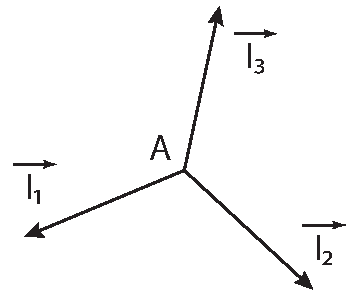
\includegraphics{cartangrp-f1}  
\end{figure}

The derivative of the vector relation
\[
\overrightarrow{\mathbf{AM}}=x\vec{ \mathbf{I}}_{1}+y\ivec_{2}+z \ivec_{3}
\]
shows that the velocity of $\mathbf{M}$ is \footnote{$\dfrac{d{\rvec{A}}}{dt}$ is the vector whose components are the derivatives of the coordinates of ${\rvec{A}}$, and $\dfrac{d\ivec_{1}}{dt}$ is the vector whose components are the derivatives of the components of $\ivec_{1}$.}
\[
\frac{d{\rvec{M}}}{dt}=\frac{d{\rvec{A}}}{dt}+x\frac{d \ivec_{1}}{dt}+y\frac{d\ivec_{2}}{dt}+z\frac{d\ivec_{3}}{dt}.
\]

Knowledge of the velocity of each point of the solid body therefore can be deduced from the knowledge of the twelve components of the vectors
\[
\frac{d{\rvec{A}}}{dt},\qquad\frac{d\ivec_{1}}{dt},\qquad\frac{d\ivec_{2}}{dt},\qquad\frac{d\ivec_{3}}{dt}.
\]

It is inappropriate to measure these vectors with respect to a fixed trihedral $\mathbf{T}_{0}$: the values of these components will then depend on both the choice of $\mathbf{T}$ and of $\mathbf{T}_{0}$. We will measure these components with respect to $\mathbf{T}$ itself, which we take to depend on the minimal number of arbitrary parameters. We therefore write
\begin{equation}
  \label{eq:1.1}
  \left\{
    \begin{alignedat}{6}
      \frac{d{\rvec{A}}}{dt}&=&\xi_{1}\ivec_{1}&\ +\ &\xi_{2}\ivec_{2}&\ +\ &\xi_{3}\ivec_{3},\\
      \frac{d\ivec_{1}}{dt}&=&\ p_{11}\ivec_{1}&\ +\ &p_{12}\ivec_{2}&\ +\ &p_{13}\ivec_{3},\\
      \frac{d\ivec_{2}}{dt}&=&\ p_{21}\ivec_{1}&\ +\ &p_{22}\ivec_{2}&\ +\ &p_{23}\ivec_{3},\\
      \frac{d\ivec_{3}}{dt}&=&\ p_{31}\ivec_{1}&\ +\ &p_{32}\ivec_{2}&\ +\ &p_{33}\ivec_{3}.\\
    \end{alignedat}
  \right.
\end{equation}

But the cross products $\ivec_{k}\times\ivec_{l}$ are constants, from which
\[
\ivec_{k}\times d\ivec_{l}+\ivec_{l}\times d\ivec_{k}=0,
\]
i.e.,
\[
p_{kl}+p_{ik}=0.
\]

Then the formula \eqref{eq:1.1} becomes
\begin{equation}
  \label{eq:1.2}
  \left\{
    \begin{alignedat}{6}
      \frac{d{\rvec{A}}}{dt}&=&\xi_{1}\ivec_{1}&\ +\ &\xi_{2}\ivec_{2}&\ +\ &\xi_{3}\ivec_{3},\\
      \frac{d\ivec_{1}}{dt}&=&&&p_{12}\ivec_{2}&\ +\ &p_{13}\ivec_{3},\\
      \frac{d\ivec_{2}}{dt}&=&\ -p_{12}\ivec_{1}& &&\ +\ &p_{23}\ivec_{3},\\
      \frac{d\ivec_{3}}{dt}&=&\ -p_{13}\ivec_{1}&\ -\ &p_{23}\ivec_{2}.\\
    \end{alignedat}
  \right.
\end{equation}

Therefore six functions $\xi_{1},\xi_{2}, \xi_{3},p_{12},p_{13},p_{23}$ are sufficient to determine the velocity of every point on the solid body at each instant $t$. Furthermore, we know that these velocities are obtained when we simultaneously apply the translation defined by the vector $(\xi_{1},\xi_{2},\xi_{3})$ and the rotation defined by the vector $(p_{23},-p_{13},p_{12})$.

\paragraph{Movements depending on several parameters.}
\label{sec:3}
The consideration in \fsref{2} has applications in many diverse questions in geometry. It is useful to generalise it so as to extend its field of applications. Therefore, let us consider a trihedral $\mathbf{T}$ depending \footnote{We always restrict ourselves to the case where the set of values of the parameters constitute a domain and the coordinates of different points of this trihedral are functions of continuous parameters and their first and second derivatives.} on $\rho$ parameters $u_{1}$, $\dots$, $u_{\rho}$. Let $\mathbf{M}$ be a fixed point associated with this trihedral. We have
\[
\overrightarrow{\mathbf{AM}}=x\ivec_{1}+y\ivec_{2}+z\ivec_{3},
\]
$x$, $y$, $z$ being three constants. There exists $\rho$ systems of relations such as the following
\begin{equation}
  \label{eq:1.3}
  \left\{
    \begin{alignedat}{6}
      \frac{\pd {\rvec{M}}}{\pd u_{q}}&=\frac{\pd {\rvec{A}}}{\pd u_{q}}&{}+x\frac{\pd \ivec_{1}}{\pd u_{q}}&&{}+y\frac{\pd \ivec_{2}}{\pd u_{q}}&&{}+z\frac{\pd \ivec_{3}}{\pd u_{q}},\\
      \frac{\pd A}{\pd u_{q}}&=&{}\xi_{1q}\ivec_{1}&&{}+\xi_{2q}\ivec_{2}&&{}+\xi_{3q}\ivec_{3},\\
      \frac{\pd \ivec_{1}}{\pd u_{q}}&=&&&{}p_{12q}\ivec_{2}&&{}+p_{13q}\ivec_{3},\\
      \frac{\pd \ivec_{2}}{\pd u_{q}}&=&{}-p_{12q}\ivec_{1}&&&&{}+p_{23q}\ivec_{3},\\
      \frac{\pd \ivec_{3}}{\pd u_{q}}&=&{}-p_{13q}\ivec_{1}&&{}-p_{23q}\ivec_{2}&.&
    \end{alignedat}
  \right.
\end{equation}

The use of differential notation permits us to condense these $\rho$ systems into one. Set
\begin{align*}
  d{\rvec{M}}&=\frac{\pd{\rvec{M}}}{\pd u_{1}}du_{1}+\frac{\pd{\rvec{M}}}{\pd u_{2}}du_{2}+\dots+\frac{\pd{\rvec{M}}}{\pd u_{\rho}}du_{\rho},\\
  &\dots\\
  d\ivec_{3}&=\frac{\pd\ivec_{3}}{\pd u_{1}}du_{1}+\frac{\pd \ivec_{3}}{\pd u_{2}}du_{2}+\dots+\frac{\pd \ivec_{3}}{\pd u_{\rho}}du_{\rho}.
\end{align*}

The system becomes
\begin{equation}
  \label{eq:1.4}
  \left\{
    \begin{alignedat}{6}
      d{\rvec{M}}&=d{\rvec{A}}&{}+x\,d\ivec_{1}&&{}+y\,d\ivec_{2}&&{}+z\,d\ivec_{3},\\
      d{\rvec{A}}&=&\omega_{1}\ivec_{1}&&{}+\omega_{2}\ivec_{2}&&{}+\omega_{3}\ivec_{3},\\
      d\ivec_{1}&=&&&{}\omega_{12}\ivec_{2}&&{}+\omega_{13}\ivec_{3},\\
      d\ivec_{2}&=&-\omega_{12}\ivec_{1}&&&&{}+\omega_{23}\ivec_{3},\\
      d\ivec_{3}&=&-\omega_{13}\ivec_{1}&&{}-\omega_{23}\ivec_{2}&.&
    \end{alignedat}
  \right.
\end{equation}

The $\omega$ are linear homogeneous forms in $du_{q}$, whose coefficients are functions of $u_{q}$. These forms are called \emph{Pfaffian forms}.  We call the preceding equations \emph{the relative components of an infinitesimal displacement of a trihedral.}

Think of $du_{q}$ as infinitesimally small for a moment and suppose all of these forms are zero except $\omega_{1}$. The displacement of $\textbf{M}$ is the translation parallel to $\ivec_{1}$ of magnitude $\omega_{1}$. Now suppose that all of the forms are zero except $\omega_{12}$. The displacement of $M$ is then, up to an infinitesimal quantity of second order, the rotation around the axis $\ivec_{3}$ of angle $\omega_{12}$. The formulae \eqref{eq:1.4} therefore show how the most general infinitesimal displacement is obtained by superimposing three infinitesimal translations parallel to the three edges of $T$ and three infinitesimal rotations around these edges.

\paragraph{The relative components have a geometrical meaning.}
\label{sec:4}
Consider a family of trihedrals depending on one or several parameters $u_{1}$, $\dots$, $u_{\rho}$. The Pfaffian forms $\omega_{1}$, $\dots$, $\omega_{23}$ are completely determined by the data of the trihedrals corresponding to the values $(u_{q})$ and $(u_{q}+du_{q})$ of the parameters. They depend only on the relative position of these two trihedrals and their values remain the same when we apply a displacement to the family of trihedrals together or when we change our choice of parameters.

The functions $\xi_{iq}$ and $p_{ijq}$ depend on the relative positions of these trihedrals and on the chosen parameters. Then, in every equation where none of these parameters has been specified, their use is less convenient than the forms $\omega$. We will therefore use the latter systematically. This geometrical meaning of the components $\omega$ has \emph{an important consequence}: consider two equal families of trihedrals and consider two trihedrals $\mathbf{T}_{1}$ and $\mathbf{T}_{2}$ in the first family corresponding to the values $(u_{q})$ and $(u_{q}+du_{q})$ of the parameters. Let $\mathbf{T}^{\star}_{1}$ and $\mathbf{T}^{\star}_{2}$ be the corresponding trihedrals in the second family and $(v_{q})$ and $(v_{q}+dv_{q})$ their parameters. The figure $(\mathbf{T}_{1},\mathbf{T}_{2})$ is equal to the figure $(\mathbf{T}^{\star}_{1},\mathbf{T}^{\star}_{2})$, and $\mathbf{T}_{2}$ is placed with respect to $\mathbf{T}_{1}$ as $\mathbf{T}^{\star}_{2}$ is with respect to $\mathbf{T}^{\star}_{1}$. From this, it follows the equality
\begin{equation}
  \label{eq:1.5}
  \left\{
    \begin{aligned}
      \omega_{i}(u;du)&=\omega_{i}(v;dv),\\
      \omega_{ji}(u;du)&=\omega_{ji}(v;dv).
    \end{aligned}
  \right.
\end{equation}

\paragraph{An integration problem.}
\label{sec:5}
Now we are going to find if the converse of this proposition holds and to tackle the following integration problem: finding all families of trihedrals corresponding to the forms $\omega_{i}$, $\omega_{ij}$ given \emph{a priori}. We will see at the beginning of the third part of this course that the forms $\omega$ are subject to certain compatibility conditions when the family of trihedrals depend on more than one parameters. We say that the \emph{structure} of these forms are not arbitrary and we name these conditions the structure equations.

We first consider the families depending one parameter $t$: hence suppose that we are given the forms \footnote{We assume that the functions $\xi_{i}(t)$ and $p_{ji}(t)$ are defined for all real values of $t$ and they admit continuous first order derivatives.}
\[
\omega_{i}=\xi_{i}(t)dt,\qquad
\omega_{ji}=p_{ji}(t)dt,\qquad
(i=1,2,3;j<i).
\]
We claim that to these there correspond families of trihedrals and these families are all equal. According to the previous paragraph this proposition is equivalent to the following: there exists one and only one family of trihedrals $\mathbf{T}$ admitting these forms as the components of their infinitesimal displacement and whose element corresponding to $t=0$ is an \emph{a priori} given trihedral. Let us choose this trihedral as the reference trihedral and adopt the following notation
\begin{alignat*}{3}
  x,y,z&\text{ are the coordinates of the point $\mathbf{A}$, the apex of the trihedral }&&\mathbf{T},\\
  \alpha,\beta,\gamma&\text{ are the components of the first vector, }&&\ivec_{1},\\
  \alpha',\beta',\gamma'&\text{ are the components of the second vector, }&&\ivec_{2},\\
  \alpha'',\beta'',\gamma''&\text{ are the components of the third vector, }&&\ivec_{3}.
\end{alignat*}
We obtain three systems of relations linking these unknowns by considering successively the components along the three axes of the coordinates of the vectors appearing in the system \eqref{eq:1.2}. The first of these systems is
\begin{equation}
  \label{eq:1.2-1}\tag{2$_{1}$}
  \left\{
    \begin{alignedat}{4}
      \frac{dx}{dt}&={}&\xi_{1}\alpha&&{}+\xi_{2}\alpha'&+\xi_{3}\alpha'',\\
      \frac{d\alpha}{dt}&={}&&&p_{12}\alpha'&+p_{13}\alpha'',\\
      \frac{d\alpha'}{dt}&={}&-p_{12}\alpha&&&+p_{23}\alpha'',\\
      \frac{d\alpha''}{dt}&={}&-p_{13}\alpha&&{}-p_{23}\alpha'.&
    \end{alignedat}
  \right.
\end{equation}
This system \eqref{eq:1.2-1} admits only one solution such that we have for $t=0$
\[
x=0,\quad\alpha=1,\quad\alpha'=0,\quad\alpha''=0.
\]
By doing the same for the other two systems, we see that there exists only one trihedral depending on $t$ that satisfies \eqref{eq:1.2} and coincides with the reference trihedral on $t=0$. It remains to verify that this variable trihedral is rectangular and that the vectors $\ivec_{1}$, $\ivec_{2}$, $\ivec_{3}$ are of unit length. We deduce from \eqref{eq:1.2} the six relations (where $p_{ij}=-p_{ji}$)
\[
\frac{d(\ivec_{i}\times\ivec_{j})}{dt}=\sum_{k=1}^{3} p_{ik}\ivec_{i}\times\ivec_{k}+\sum_{k=1}^{3}p_{jk}\ivec_{j}\times\ivec_{k}.
\]

These relations constitute a linear system with respect to the six quantities $\ivec_{i}\times\ivec_{j}$. The only solution satisfying the given initial values imposed is obvious and it is
\[
{\ivec_{1}}^{2}=
{\ivec_{2}}^{2}=
{\ivec_{3}}^{2}=1,\qquad
\ivec_{1}\times\ivec_{2}=
\ivec_{2}\times\ivec_{3}=
\ivec_{3}\times\ivec_{1}=0.
\]
The proposition is then established.

\paragraph{Equality of two $\rho$-parameter families having the same relative components.}
\label{sec:6}
Let us finish proving the converse of \fsref{4} [formulae \eqref{eq:1.5}]: consider two families of trihedrals $\mathbf{T}$ and $\mathbf{T}^{\star}$ depending on $\rho$ parameters $u_{1}$, $u_{2}$, $\dots$, $u_{\rho}$ and $v_{1}$, $v_{2}$, $\dots$, $v_{\rho}$ respectively and suppose that a continuous and bijective correspondance established between $\mathbf{T}$ and $\mathbf{T}^{\star}$ realises the equalities
\begin{equation}
  \label{eq:1.5a}\tag{\ref{eq:1.5}}
  \left\{
    \begin{aligned}
      \omega_{i}(u;du)&=\omega^{\star}_{i}(v;dv),\\
      \omega_{ji}(u;du)&=\omega^{\star}_{ji}(v;dv).
    \end{aligned}
  \right.
\end{equation}

Let us choose two trihedrals $\mathbf{T}_{1}$ and $\mathbf{T}_{2}$ in the first family and let $\mathbf{T}_{1}^{\star}$ and $\mathbf{T}_{2}^{\star}$ be their analogues in the second family. We can find \footnote{Since the families are assumed to be connected [note in \fsref{3}].} a family of trihedrals depending on one parameter $\mathbf{T}_{3}$ belonging to the first family such that $\mathbf{T}_{3}$ coincides with $\mathbf{T}_{1}$ at $t=0$ and with $\mathbf{T}_{2}$ at $t=1$. Let $\mathbf{T}_{3}^{\star}$ be the analogous trihedral of $\mathbf{T}_{3}$. The components $\omega^{\star}$ of the infinitesimal displacement of $\mathbf{T}_{3}^{\star}$ are equal to the components $\omega$ of the infinitesimal displacement of $\mathbf{T}_{3}$. The preceding paragraph affirms that under these conditions the displacement which makes $\mathbf{T}_{1}$ and $\mathbf{T}_{1}^{\star}$ superimpose the corresponding $\mathbf{T}_{3}$ and $\mathbf{T}_{3}^{\star}$, and hence in particular $\mathbf{T}_{2}$ and $\mathbf{T}_{2}^{\star}$. But as $\mathbf{T}_{2}$ and $\mathbf{T}_{2}^{\star}$ are two arbitrary elements of the families $\mathbf{T}$ and $\mathbf{T}^{\star}$, this displacement superimpose all corresponding elements of the two families $\mathbf{T}$ and $\mathbf{T}^{\star}$.\qed

We state the conclusions of \fsref{4} and \fsref{6}

\paragraph{The fundamental condition of equality.}
\label{sec:7}
\emph{Consider a bijective correspondance established between two $\rho$ parameter families of trihedrals $\mathbf{T}$ and $\mathbf{T}^{\star}$. For a single displacement to suffice to superimpose all the corresponding trihedrals, it is necessary and sufficient that the correspondance in question makes the components $\omega$ of infinitesimal displacement of $\mathbf{T}$ equal to the components $\omega^{\star}$ of the infinitesimal displacement of the analogous $\mathbf{T}^{\star}$.}

We note on the other hand the conclusion of \fsref{5}.

\theoremstyle{shape1}
\newtheorem*{strthm}{Structure theorem}
\begin{strthm}
  The components of the infinitesimal displacement of a moving rectangular trihedral depending on one parameter are not subject to any structure conditions \emph{(in other words: these components are the formes in one completely arbitrary variable)}.
\end{strthm}

\paragraph{Remark concerning \fsref{5}.}
\label{sec:8}
In the course of this paragraph we have characterised the position of an arbitrary trihedral in space with the help of $12$ parameters linked by $6$ relations: the parameters are $x$, $y$, $z$, $\alpha$, $\beta$, $\gamma$, $\alpha'$, $\beta'$, $\gamma'$, $\alpha''$, $\beta''$, $\gamma''$ and the relations are $\alpha^{2}+\beta^{2}+\gamma^{2}=1$, $\alpha\alpha'+\beta\beta'+\gamma\gamma'=0$, $\dots$

It follows from these complications that are not conducive to generalisations, as we have seen. Therefore let us utilise six independent parameters to define a trihedral. These are, for example, the three coordinates of the apex and the three Euler angles $(\phi, \theta, \psi)$ and let us prove a new conclusion of \fsref{5}.

``We can choose in one and only one way the parameters $x$, $y$, $z$, $\phi$, $\theta$, $\psi$ as functions of one parameter $t$ such that the trihedral has at $t=0$ a fixed position and the components of its infinitesimal displacement $\omega_{i}$, $\omega_{ji}$ $(j<i)$ are equal to given forms $\xi_{i}(t)dt$, $p_{ji}(t)dt$.''

Suppose that $\omega_{i}$ and $\omega_{ji}$ $(j<i)$ are independent forms in the six differentials $dx$, $dy$, $dz$, $d\phi$, $d\theta$, $d\psi$. The system
\[
\omega_{i}=\xi_{i}(t)dt,\qquad\omega_{ji}=p_{ji}(t)dt
\]
is equivalent to a system of six differential equations
\begin{align*}
  \frac{dx}{dt}&=f_{1}(x,y,z,\phi,\theta,\psi,t),\quad&
  \frac{d\phi}{dt}&=f_{4}(x,y,z,\phi,\theta,\psi,t),\\
  \frac{dy}{dt}&=f_{2}(x,y,z,\phi,\theta,\psi,t),\quad&
  \frac{d\theta}{dt}&=f_{5}(x,y,z,\phi,\theta,\psi,t),\\
  \frac{dz}{dt}&=f_{3}(x,y,z,\phi,\theta,\psi,t),\quad&
  \frac{d\psi}{dt}&=f_{6}(x,y,z,\phi,\theta,\psi,t).  
\end{align*}
This system admits one and only one solution corresponding to the values of the unknowns given at $t=0$. The proposition is hence established.

But the hypothesis that the six forms $\omega_{i}$, $\omega_{ji}$ are dependent is absurd. We may then actually find a differential system
\[
\frac{dx}{g_{1}(x,y,z,\phi,\theta,\psi)}=\frac{dy}{g_{2}}=\frac{dz}{g_{3}}=\frac{d\phi}{g_{4}}=\frac{d\theta}{g_{5}}=\frac{d\psi}{g_{6}},
\]
whose integrals annihilate these six forms: there exists moving trihedrals whose components of infinitesimal displacement are zero, and each point of it is then fixed. This is absurd.

The conclusion of \fsref{5} can also be established by a second, less complicated and better reasoning. It is interesting to note that we just used the components of infinitesimal displacement of a most general trihedral in the question relative to the families of trihedrals depending on a single parameter.

\section[{Application of the theory of one-parameter families of trihedrals to space curves}]{Application of the theory of one-parameter families of trihedrals to the study of space curves}
\label{sec:appl-theory-one}

\paragraph{The various geometrical elements attached to a curve.}
\label{sec:9}
We will now rapidly review the classical theory of space curves. Consider a real space curve $C$. We start by define at each of its point, with the help of various infinitesimal geometrical constructions, the \emph{tangent}, the differential of the \emph{arc} $ds$, and to choose the sign of $ds$ it is necessary to \emph{orient} the curve. We then define the \emph{osculating plane}, the \emph{principal normal} and the \emph{binormal}.

Observe that the tangent is a first order geometrical element, that the osculating plane, the principal normal and the binormal are second order geometrical elements \footnote{In our study we exclude the inflection points of $C$.}. This simply signifies that two curves having a first order contact have the same tangent, and they have the same osculating plane, principal normal, binormal when they have a second order contact. Recall that the set of curves having a $P$-th order contact between any two of them at a given point constitute a \emph{$P$-th order contact element}, and this element is sait to belong to each of these curves. Suppose that the curve considered are defined by the functions $y(x)$ and $z(x)$ and their tangents are not parallel to the $yz$ plane. A $P$-th order contact element can be characterised analytically by the data of one value of $x$ and the corresponding values taken by the functions
\[
y(x),\quad z(x),\quad \frac{dy}{dx},\quad \frac{dz}{dx},\quad\dots,\quad\frac{d^{P}y}{dx^{P}},\quad \frac{d^{P}z}{dx^{P}}.
\]
The quantity $ds$ is an \emph{first order differential element}: this signifies that it is expressed by means of $dx$ and the coordinates of the first order contact element.

\paragraph{The relative components of the displacement of Frenet trihedral.}
\label{sec:10}
Consider the right rectangular trihedrals $\mathbf{A}\ivec_{1}\ \ivec_{2}\ \ivec_{3}$ at each point $\mathbf{A}$ of the curve $C$ having the following properties: the orthogonal vectors $\ivec_{1}$, $\ivec_{2}$, $\ivec_{3}$ are of length $1$, $\ivec_{1}$ is along the positive tangent, $\ivec_{2}$ is along the principal normal and $\ivec_{3}$ is along the binormal. At each point of $\mathbf{M}$ we then find two trihedrals attached and we go from one of them to the other by changing $\ivec_{2}$ to $-\ivec_{2}$ and $\ivec_{3}$ to $-\ivec_{3}$.

When $\mathbf{M}$ traces the curve $C$, each of these trihedrals generate a connected family of trihedrals. These trihedrals are second order geometrical elements.

Let us introduce the relative components $\omega$ of the infinitesimal displacement of these trihedrals. The definition of the tangent is expressed by the relations $\omega_{2}=0$, $\omega_{3}=0$, that of $ds$ by the relation $\omega_{1}=ds$, that of the principal normal by the relation $\omega_{13}=0$, and $\omega_{12}$, $\omega_{13}$ are of the form $\omega_{12}=\rho\,ds$, $\omega_{23}=\tau\,ds$, $\rho$ and $\tau$ being functions in $s$. Under these conditions the formulae \eqref{eq:1.4} furnish the \emph{Frenet formulae}
\begin{equation}
  \label{eq:1.6}
  \left\{
    \begin{alignedat}{3}
      d{\rvec{A}}&=&ds\,\ivec_{1},\\
      d\ivec_{1}&=&&&\rho\,ds\,\ivec_{2},\\
      d\ivec_{2}&={}&-\rho\,ds\,\ivec_{1}&&&+\tau\,ds\,\ivec_{3},\\
      d\ivec_{3}&=&&&-\tau\,ds\,\ivec_{2}.
    \end{alignedat}
  \right.
\end{equation}

If we use the other trihedral $\mathbf{M}\ \ivec_{1}\ \ivec_{2}\ \ivec_{3}$, $\rho$ will be changed to $-\rho$ whereas $\tau$ retains the same value. For one of these trihedrals $\rho$ is therefore positive, and we will name this one the \emph{Frenet trihedral}, and its determination requires only the knowledge of second order contact elements, and hence we will also call the trihedral \emph{second order trihedral}. We will apply the Frenet formulae \eqref{eq:1.6} to this trihedral. The functions $\rho$ and $\tau$, which have intrinsic meaning, are the curvature and torsion. We will call them the second order and third order invariants.

Frenet formulae allows us to readily calculate $\rho$ and $\tau$ by derivation when we know the explicit equations of $C$. They show that if we change the orientation of $C$, $\rho$ and $\tau$ will retain the same values, whereas $ds$ will be multiplied by $-1$. They provide the geometrical interpretation of $\rho$ and $\tau$. Finally, note that they permit us to calculate, at a point $\mathbf{A}$,
\begin{align*}
  \frac{d{\rvec{A}}}{ds}&\text{ when we know on the point: } \ivec_{1},\\
  \frac{d^{2}{\rvec{A}}}{ds^{2}}&\text{ when we know on the point: } \ivec_{1}, \rho,\\
  \frac{d^{3}{\rvec{A}}}{ds^{3}}&\text{ when we know on the point: } \ivec_{1},\ivec_{2},\ivec_{3},\rho,\frac{d\rho}{ds},\tau,\\
  \frac{d^{P}{\rvec{A}}}{ds^{P}}&\text{ when we know on the point: } \ivec_{1},\ivec_{2},\ivec_{3},\rho,\dots,\frac{d^{P-2}\rho}{ds^{P-2}},\tau,\dots,\frac{d^{P-3}\rho}{ds^{P-3}}.
\end{align*}


\paragraph{}
\label{sec:11}
The preceding results are sufficient to resolve two questions that arise naturally:
\newtheorem*{pcont}{Contact problem}
\begin{pcont}
  Given an integer $P$, two real curves $C$ and $C^{\star}$ and two points on these curves $\mathbf{A}_{0}$ and $\mathbf{A}^{\star}_{0}$, find all displacements transforming $\mathbf{A}_{0}^{\star}$ to $\mathbf{A}_{0}$ and $C^{\star}$ into a curve having at $\mathbf{A}_{0}$ with the curve $C$ a contact of order at least equal to $P$.
\end{pcont}

\newtheorem*{pequ}{Equality problem}
\begin{pequ}
  Find all the displacements that superimpose two given real curves $C$ and $C^{\star}$.
\end{pequ}

It will be \emph{convenient} for us to say that two \emph{oriented} curves have an order $P$ contact at a point only in the following case: they have at this point such a contact (here we abstract away their orientations), and moreover their positive tangents coincide at this point. Similarly a displacement will be said to superimpose two oriented curves only if it superimposes the two curves as well as their orientation.

The solutions of the contact problem consists of the solutions of two contact problems relative to the curve $C$ oriented arbitrarily and the curve $C^{\star}$ oriented in one or the other sense. Similarly the equality problem decomposes into two equality problems relative to the oriented curves. It is the problems relative to oriented curves that we are going to learn to solve.

\paragraph{Contact problem of two oriented curves.}
\label{sec:12}
First suppose $P\ge 2$. We exclude the case where one of the points $\mathbf{A}_{0}$, $\mathbf{A}_{0}^{\star}$ is an infection point. Let us choose these points as the origins of the curvilinear abscissas. If the problem is solvable, the displacement we are searching for superimpose the two Frenet trihedrals with apexes $\mathbf{A}_{0}$ and $\mathbf{A}_{0}^{\star}$, and moreover the elements of order up to $P$:
\[
\rho,\quad\dots\quad\frac{d^{P-2}\rho}{ds^{P-2}},
\]
and, if $P>2$,
\[
\tau,\quad\dots\quad\frac{d^{P-3}\tau}{ds^{P-3}},
\]
each take the same value on the two points. Conversely suppose that this displacement is applied and these conditions are satisfied. Let $\mathbf{A}$ and $\mathbf{A}^{\star}$ be the two points on $C$ and the displaced curve $C^{\star}$, whose curvilinear abscissas are both equal to $s$. According to the last line of \fsref{10}, we have on $s=0$,
\[
\mathbf{A}=\mathbf{A}^{\star},\quad\frac{d{\rvec{A}}}{ds}=\frac{d{\rvec{A}}^{\star}}{ds},\quad\dots\quad\frac{d^{P}{\rvec{A}}}{ds^{P}}=\frac{d^{P}{\rvec{A}}^{\star}}{ds^{P}}.
\]

Taylor's formula permits us to deduce from these equations that when $s$ tends to zero, $\dfrac{\overline{\mathbf{AA}^{\star}}}{s^{P+1}}$ remains bounded: the two curves have a contact of order at least equal to $P$.

Hence for the problem to be solvable, it is necessary and sufficient that each of the elements $\rho$, $\dfrac{d\rho}{ds}$, $\dots$; $\tau$, $\dfrac{d\tau}{ds}$, $\dots$, whose order is at least equal to $P$, to have the same value at $\mathbf{A}_{0}$ and $\mathbf{A}_{0}^{\star}$. If the problem is solvable, the displacement we are looking for is unique: it is the one that superimpose the two second order trihedrals at $\mathbf{A}_{0}$ and $\mathbf{A}_{0}^{\star}$.

\somespace

\emph{Case where $P=1$}. The problem is always solvable. For enunciating the solutions as in the case where $P\ge 2$, let us use the following definition: a right rectangular trihedral $\mathbf{A}\ivec_{1}\ \ivec_{2}\ \ivec_{3}$ will be called a \emph{first order trihedral} attached at a point $\mathbf{A}$ of a (oriented) curve when $\ivec_{1}$ is along the (positive) tangent of the point $\mathbf{A}$. The displacements we search for are those that superimpose a particular first order trihedral attached at $\mathbf{A}_{0}^{\star}$ unto the most general first order trihedral attached at $\mathbf{A}_{0}$.

\paragraph{Equality problem.}
\label{sec:13}
When $C$ and $C^{\star}$ are analytic the equality problem can be resolved by an intermediate contact problem: the necessary and sufficient condition for a displacement which makes the points $\mathbf{A}_{0}$ and $\mathbf{A}_{0}^{\star}$ superimposes the curves $C$ and $C^{\star}$ is that which realises at these points a contact of order larger than every integer $P$. Using the conclusion of the preceding paragraph and noting that $\rho$ and $\tau$ are analytic functions of $s$, we obtain the following solvability condition: the curvature $\rho$ and the torsion $\tau$ must each be the same function of the curvilinear abscissas $s$ along the two curves.

However, it is preferable to tackle the problem differently. We now only suppose that the coordinates of a point along the curve are functions of a parameter admitting fourth order derivatives. The problem of superimposing two oriented curves $C$ and $C^{\star}$ is equivalent to the problem of superimposing the families of Frenet trihedrals attached to these curves.

The fundamental condition for equality (\fsref{7}, p.~\pageref{sec:7}) applies: this makes the problem into the search for all correspondances between the curvilinear abscissas $s$ and $s^{\star}$ of the two curves realising the three equalities
\[
ds=ds^{\star},\qquad\rho(s)ds=\rho^{\star}(s^{\star})ds^{\star},\qquad\tau(s)ds=\tau^{\star}(s^{\star})ds^{\star}.
\]

The search for these correspondances proceed as the following:

Two cases can be distinguished:
\begin{enumerate}
\item \emph{$\rho$ and $\tau$ are constants}. It it then necessary that $\rho^{\star}$ and $\tau^{\star}$ have the same constant values. This is also sufficient, and there exists an infinite number of correspondances, namely $s=s^{\star}+C$ where $C$ denote an arbitrary constant. Each of the two curves can slide along themselves by a continuous displacement.
\item \emph{$\rho$ and $\tau$ are not both constants}. Suppose for example the curvature to be non-constant. Let $\dfrac{d\rho}{ds}=F(\rho)$, $\tau=\Phi(\rho)$. It is then necessary to have $\dfrac{d\rho^{\star}}{ds^{\star}}=F(\rho^{\star})$, $\tau^{\star}=\Phi(\rho^{\star})$ with the same functions $F$ and $\Phi$. This condition is sufficient: if indeed we establish between $s$ and $s^{\star}$ the correspondance given by $\rho(s)=\rho\str(s\str)$ and
\[
ds=\frac{d\rho}{F(\rho)}=\frac{d\rho\str}{F(\rho\str)}=ds\str.
\]
\end{enumerate}

\paragraph{}
\label{sec:14}
Finally, let us use the structure theorem stated in \fsref{7}. We have determined that, whatever the functions $\rho(s)$ and $\tau(s)$, there corresponds to them two families of trihedrals, equal between the two families, depending on the parameter $s$ and satisfying the equations \eqref{eq:1.6}. Let $C$ be the position of the apex $\mathbf{A}$ of these trihedrals. The equations \eqref{eq:1.6} prove that the trihedrals are the Frenet trihedrals at $C$. Then:
\begin{strthm}
  The curvature and the torsion of a space curve are arbitrary functions of the arc length.
\end{strthm}


\section{Study of space curves based on the theory of multi-parameter families of trihedrals}
\label{sec:study-space-curves}

\paragraph{Introduction.}
\label{sec:15}
In the course of the preceding paragraph, the two problems of contact and of equality have not been analysed: they are found to be solved by a series of doubtlessly ingenious considerations, but which are also difficult to generalise. We are going to take up the study of them again by a more systematic method, which will prove easy to apply to numerous problems of the same nature but which are more complicated than our treatment in the preceding.

We are first concerned with the contact problem. We will learn to solve them recurrently order by order. This solution will lead us to define successively the various order elements attached at a point on a real curve. With the help of these elements, we will state the solvability conditions and we will define their solutions. After the contact problem has been completely treated, we will find ourselves to have sufficient knowledge to solve the equality problem.

\paragraph{Principle of recurrent solution of the contact problem.}
\label{sec:16}
The most general order $P$ contact element depends on $2P+3$ parameters $[x,y,z,\dots,y^{(P)},z^{(P)}]$. We can therefore envisage it as a point in a $2P+3$ dimensional space. There then correspond to a order $P$ contact element of a curve $C$ a curve $\Gamma$ in a $2P+3$ dimensional space. For two curves $C$ and $C\str$ of the three dimensional space to have a contact of at least order $P$, it is necessary and sufficient that the corresponding curves $\Gamma$ and $G\str$ have a point in common: for the order of the contact to be greater than $P$ it is necessary and sufficient that $\Gamma$ and $\Gamma\str$ are tangent at this point. Indeed, for the last two curves to be tangent, it is necessary and sufficient that at the common point of abscissa $x$, the other coordinates $y$, $z$, $y'$, $z'$, $\dots$, $y^{(P)}$, $z^{(P)}$, considered as functions in $x$, are equal as well as their first derivatives, but this signifies the one-to-one equality of the quantities $y$, $z$, $y'$, $z'$, $\dots$, $y^{(P)}$, $z^{(P)}$, $y^{(P+1)}$, $z^{(P+1)}$ and $y\str$, $z\str$, $y^{\star\prime}$, $\dots$, $y^{\star(P)}$, $z^{\star(P)}$, $y^{\star(P+1)}$, $z^{\star(P+1)}$, or in other words, that the two given curves $C$ and $C\str$ have a order $P+1$ contact.

We can now make the contact condition of two curves $\Gamma$ and $\Gamma\str$ under another form by expressing that there exists two points $\alpha$, $\alpha\str$ on the two curves infinitesimally close to the common point $\alpha_{0}$ and the distance between them is zero up to an infinitesimally small error as measured against the distance between $\alpha_{0}$ and $\alpha$. We deduce from this the following contact condition for the curve $C$.
\theoremstyle{shapesc}
\newtheorem*{contactcon}{Contact condition}
\begin{contactcon}
  The necessary and sufficient condition for two curves $C$ and $C\str$ having a point $\mathbf{A}_{0}$ in order $P$ order contact to have a order $\ge P+1$ contact at the point is the following: there must exist on $C$ a point $\mathbf{A}$ and on $C\str$ a point $\mathbf{A}\str$ which are infinitesimally close to $\mathbf{A}_{0}$ for which the relations expressing that $C$ and $C\str$ have a contact of order $\ge P$ at $\mathbf{A}$ and $\mathbf{A}\str$ are realised up to infinitesimally small errors compared with the distance between $\mathbf{A}_{0}$ and $\mathbf{A}$.
\end{contactcon}

The contact problem therefore will be treated by a recurrent procedure: to solve the contact problem of order $P+1$ we search among the solutions of the order $P$ problem those solutions that satisfy the condition that we just stated.

For brevity, \emph{assume that we have already solved the first order contact problem} and defined for this purpose the tangent and first order trihedrals (\emph{see} the end of \fsref{12}). We also assume the orientation to be already defined and we only consider the problems relative to oriented curves. A oriented contact element is characterised by the associated connected family of first order trihedrals and it is completely determined by one of these trihedrals. The first order trihedrals of a curve depend on two parameters: we utilise one parameter $t$ characterising the position of the apex of the trihedral on the curve, which we name the \emph{principal parameter}, and one \emph{secondary parameter} $\theta$ which is the angle that we need to turn the trihedral $(t,0)$ around the positive tangent to obtain the trihedral $(t,\theta)$. The sufficient condition for first order contact of two curves is that a particular first order trihedral of the first curve is also a first order trihedral of the second curve.

\paragraph{Application of the contact condition to the problem of second order contact.}
\label{sec:17}
Consider a displacement resolving the first order problem: it superimposes an arbitrary first order trihedral $\mathbf{T}\str_{0}$ attached to $\mathbf{A}_{0}\str$ to a certain first order trihedral $\mathbf{T}_{0}$ attached at $\mathbf{A}_{0}$. Call the parameters of the trihedrals $(t\str_{0},\theta\str_{0})$ and $(t_{0},\theta_{0})$. For the displacement to solve the second order contact problem, it is necessary and sufficient that given a first order trihedral $\mathbf{T}\str$ of $C\str$ infinitesimally close to $\mathbf{T}\str_{0}$ whose apex is a point $\mathbf{A}\str$ infinitesimally close to $\mathbf{A}\str_{0}$, we can find a first order trihedral $\mathbf{T}$ on $C$ that the displacement considered superimposes it unto $\mathbf{T}\str$ up to infinitesimally small quantities compared to $\overline{\mathbf{A}\str_{0}\mathbf{A}_{\vphantom{0}}^{\star}}$. This condition is analytically expressed as follows:

\somespace

Let $\omega_{i}(t,\theta,dt,d\theta)$, $\omega_{ij}(t,\theta,dt,d\theta)$; $\omega_{i}\str(t\str,\theta\str,dt\str,d\theta\str)$, $\omega_{ij}\str(t\str,\theta\str,dt\str,d\theta\str)$ be the components of infinitesimal displacement  of a first order trihedral of $C$ and $C\str$. The system
\begin{equation}
  \label{eq:1.c}\tag{$c$}
  \left\{
    \begin{aligned}
      \omega_{i}(t_{0},\theta_{0},dt,d\theta)&=\omega_{i}(t_{0},\theta_{0},dt,d\theta),&&(i=1,2,3),\\
      \omega_{ji}(t_{0},\theta_{0},dt,d\theta)&=\omega_{ji}(t_{0},\theta_{0},dt,d\theta),&&(j<i),
    \end{aligned}
  \right.
\end{equation}
where $dt\str$ and $d\theta\str$ are given, must admit a solution in $dt$ and $d\theta$.

\somespace

The contact problem to solve is therefore equivalent to the following problem: associate to a value $\theta_{0}\str$ chosen according to our convenient all the values of $\theta_{0}$ realising the condition \eqref{eq:1.c}.

\paragraph{Details of the nature of the forms $\omega_i$, $\omega_{ji}$.}
\label{sec:18}
The movement of the trihedral of parameters $(t,\theta)$ is completely determined by the knowledge of $\theta$ and the movement of the trihedral $(t,0)$. It is therefore natural to learn to calculate the forms $\omega(t,\theta,dt,d\theta)$ as functions of the forms $\omega(t,0,dt,0)$, $\theta$ and $d\theta$. This is what we are going to do. For this, observe that we have, according to the formula \eqref{eq:1.4} on page \pageref{eq:1.4} and the definition of first order trihedral,
\begin{equation}
  \label{eq:1.7}
  \left\{
    \begin{aligned}
      \omega_{1}(t,\theta,dt,d\theta)&=\ivec_{1}\times d{\rvec{A}},\qquad\omega_{2}(t,\theta,dt,d\theta)=\omega_{3}(t,\theta,dt,d\theta)=0,\\
      \omega_{ji}(t,\theta,dt,d\theta)&=\ivec_{i}\times d\ivec_{j}.
    \end{aligned}
  \right.
\end{equation}

Denote the trihedral corresponding to $\theta=0$ by $\mathbf{A}{\jvec}_{1}{\jvec}_{2}{\jvec}_{3}$. We have
\begin{equation}
  \label{eq:1.8}
  \ivec_{1}={\jvec}_{1},\qquad\ivec_{2}={\jvec}_{2}\cos\theta+{\jvec}_{3}\sin\theta,\qquad\ivec_{3}=-{\jvec}_{2}\sin\theta+{\jvec}_{3}\cos\theta.
\end{equation}

We also have analogous formulae to \eqref{eq:1.7}:
\begin{equation}
  \label{eq:1.9}
  \left\{
    \begin{aligned}
      \omega_{1}(t,\theta,dt,d\theta)&={\jvec}_{1}\times d{\rvec{A}},\qquad\omega_{2}(t,\theta,dt,d\theta)=\omega_{3}(t,\theta,dt,d\theta)=0,\\
      \omega_{ji}(t,\theta,dt,d\theta)&={\jvec}_{i}\times d{\jvec}_{j}.
    \end{aligned}
  \right.  
\end{equation}

Let us replace the quantities $\ivec_{1}$, $\ivec_{i}$ and $d\ivec_{j}$ by their expressions from \eqref{eq:1.8}. In the formulae obtained let us use the relations \eqref{eq:1.9}, and they become
\begin{equation}
  \label{eq:1.10}
  \left\{
    \begin{aligned}
      \omega_{1}(t,\theta,dt,d\theta)&=\omega_{1}(t,0,dt,0),\\
      \omega_{2}(t,\theta,dt,d\theta)&=\omega_{3}(t,\theta,dt,\theta)=0,\\
      \omega_{12}(t,\theta,dt,d\theta)&=\omega_{12}(t,0,dt,0)\cos\theta+\omega_{13}(t,0,dt,0)\sin\theta,\\
      \omega_{13}(t,\theta,dt,d\theta)&=-\omega_{12}(t,0,dt,0)\sin\theta+\omega_{13}(t,0,dt,0)\cos\theta,\\
      \omega_{23}(t,\theta,dt,d\theta)&=d\theta+\omega_{23}(t,0,dt,0).
    \end{aligned}
  \right.
\end{equation}

The differential $d\theta$ does not appear in the forms $\omega_{1}$, $\omega_{2}$, $\omega_{3}$, $\omega_{12}$, $\omega_{13}$: these components only depend on the choice of the trihedral $(t,\theta)$ and the position of the apex of the trihedral $(t+dt,\theta+d\theta)$. We will agree in all analogous cases to call these components the \emph{principal components}.

There exists certain first order trihedrals whose matrix of principal components is particularly simple. The form $\omega_{13}$ is zero for two values of $\theta$. Let us consider \footnote{We suppose the curve to be oriented in the sense of increasing parameters and we exclude from consideration the points on which $\omega_{12}(t,0,dt,0)$ and $\omega_{13}(t,0,dt,0)$ are both zero.} the values which make the quotient $\dfrac{\omega_{12}(t,\theta,dt)}{\omega_{1}(t,\theta,dt)}$ positive, which is independent of $dt$. We call the corresponding trihedral ``the second order trihedral'' or ``the Frenet trihedral'' and the value $\rho$ corresponding to $\dfrac{\omega_{12}}{\omega_{1}}$ ``the curvature''.

On the other hand, observe that according to \eqref{eq:1.10}, the form $\omega_{1}$ is the same for every first order trihedral. It constitutes a \emph{first order differential invariant}. We call it ``the differential of the arc element'' and denote it by $ds$. Henceforth we assume that $t=s$.

The Frenet formulae [\eqref{eq:1.6}, p.~\pageref{eq:1.6}] show that these definitions correspond well to the usual definitions of the arc element and the Frenet trihedral which have been reviewed in the preceding paragraph.

\paragraph{Return to the second order contact problem (\fsref{17}).}
\label{sec:19}
Consider the condition \eqref{eq:1.c} again. Let us choose $\theta\str_{0}$ in a way that the corresponding trihedral $\mathbf{T}\str_{0}$ is the second order trihedral of the curve $C\str$ at $\mathbf{A}\str_{0}$. The condition \eqref{eq:1.c} requires $\theta_{0}$ to be such that at the point $A_{0}$ we have $\omega_{13}=0$, $\dfrac{\omega_{12}}{\omega_{1}}>0$. The trihedral $\mathbf{T}_{0}$ is therefore necessarily the second order trihedral of the curve $C$ at $\mathbf{A}_{0}$. The system which appear in the condition \eqref{eq:1.c} can now be written as
\begin{align*}
  ds&=ds\str,\\
  \rho\,ds&=\rho\str ds\str,\\
  d\theta+\omega_{23}(s,0,ds,0)&=d\theta\str+\omega_{23}\str(s\str,0,ds\str,0).
\end{align*}

The condition \eqref{eq:1.c} is equivalent to the condition $\rho=\rho\str$. The equality of two curvatures is therefore the only solvability condition of the problem. This condition, once satisfied, the problem admits a unique solution: it is the displacement which superimposes the Frenet trihedral $\mathbf{T}\str_{0}$ with the Frenet trihedral $\mathbf{T}_{0}$.

\paragraph{Third order contact problem.}
\label{sec:20}
Let us now apply the contact condition (\fsref{16}), which is very easy since the second order problem admits at most one solution. This solution, when it exists, is the displacement which superimposes the Frenet trihedral $\mathbf{A}_{0}$ and $\mathbf{A}\str_{0}$. Let us assume this. The condition for it to realise a order $\ge 3$ contact is the following: there must exist a point $\mathbf{A}$ on $C$ and a point $\mathbf{A}\str$ on $C$, infinitesimally close to $\mathbf{A}_{0}$, such that the Frenet trihedrals and the relative curvatures at these points coincide up to infinitesimally small quantities compared to $\overline{\mathbf{A}_{0}\mathbf{A}}$. This condition is equivalent to the following, where the forms $\omega$ and $\omega\str$ represent the infinitesimal displacement components of the Frenet trihedrals of the two curves: the system
\begin{align*}
  \rho+\frac{d\rho}{ds}ds&=\rho\str+\frac{d\rho\str}{ds\str}ds\str,\\
  \omega_{i}(s,ds)&=\omega\str_{i}(s\str,ds\str),\\
  \omega_{ji}(s,ds)&=\omega\str_{ji}(s\str,ds\str),
\end{align*}
must admit a solution for which neither $ds$ nor $ds\str$ is zero.

The solvability conditions of the problem is therefore
\[
\rho=\rho\str,\qquad\frac{d\rho}{ds}=\frac{d\rho\str}{ds\str},\qquad\tau=\tau\str.
\]
If these conditions are satisfied, the solution is unique.

From the above it is easy to deduce successively the solutions \emph{of order $4$, $\dots$, $P$ contact problems} [c.f. \fsref{12}, p.~\pageref{sec:12}].

\paragraph{Equality problem.}
\label{sec:21}
The family of second order trihedrals attached at an oriented curve $C$ is such that if we displace $C$ this family will transform by the same displacement. Let us recall the reasons: the family of first order trihedrals possesses this property, and moreover, a displacement does not alter the relative components $\omega$ of the infinitesimal displacement of a trihedral. The second order trihedrals are defined as first order trihedrals whose (principal) components $\omega$ satisfy certain relations.

On the other hand, the family of second order trihedrals depend on a single parameter.

Through this, the equality problem of two oriented curves then becomes the equality of two families of one-parameter trihedrals, and this problem is solved easily by the fundamental condition for equality in paragraph \fsref{7} (p.~\pageref{sec:7}) (c.f.~\fsref{13}, p.~\pageref{sec:13}).

Also, the \emph{structure theorem} of paragraph \fsref{14} (p.~\pageref{sec:14}) results immediately from the \emph{structure theorem} of paragraph \fsref{7} (p.~\pageref{sec:7}).



\section{The method of reduced equations}
\label{sec:meth-reduc-equat}

\addtocounter{paragraph}{-1}

\paragraph{\textnormal{\textit{bis.}}}
\label{sec:21a}
We can obtain the Frenet equations by another method than the one we just developed, the method of \emph{reduced equations}. Given a oriented space curve $C$, the method consists of attaching at each of its points $\mathbf{A}$ a rectangular trihedral such that the equations of the curve, which we assume to be analytic, when expanded in a neighbourhood of $\mathbf{A}$ have their first coefficients taking the simplest form possible. The $x$-axis is naturally the positive tangent here, the $y$-axis is the principal normal and the $z$-axis is the binormal. The equations of the curve is of the form
\begin{equation}
  \label{eq:1.11}
  \left\{
    \begin{aligned}      
      y&=\frac{1}{2}ax^{2}+\frac{1}{6}cx^{3}+\cdots,\\
      z&=\frac{1}{6}bx^{3}+\cdots.
    \end{aligned}      
  \right.
\end{equation}

The abscissa $x$ of a point $\mathbf{A}'$ infinitesimally close to $\mathbf{A}$ is infinitesimally small which has an intrinsic significance and which is just the arc element $ds$. The coefficients $a$ and $b$ are invariants attached at the point $A$, the first is manifestly of second order and the second third order.

The Frenet formulae give the infinitesimal displacement components $\omega_{i}$, $\omega_{ij}$ of the trihedral attached at the moving point $\mathbf{A}$ on the curve [formula \eqref{eq:1.4}, p.~\pageref{eq:1.4}]
\begin{alignat*}{4}
  d\mathbf{A}&={}&{}\omega_{1}\ivec_{1}&&{}+{}\omega_{2}\ivec_{2}&&{}+{}\omega_{3}\ivec_{3},\\
  d\ivec_{1}&=&&&\omega_{12}\ivec_{2}&&{}+{}\omega_{13}\ivec_{3},\\
  d\ivec_{2}&=&-\omega_{12}\ivec_{1}&&&&{}+{}\omega_{23}\ivec_{3},\\
  d\ivec_{3}&=&-\omega_{13}\ivec_{3}&&{}-{}\omega_{23}\ivec_{2}&.&
\end{alignat*}

Now take a fixed point $\mathbf{B}$ on the curve and let $x$, $y$, $z$ be its coordinates with respect to a trihedral $\mathbf{T}$ of the origin $\mathbf{A}$. They satisfy equation \eqref{eq:1.11} where the coefficients $a$, $b$, $\dots$, dependent on $\mathbf{A}$, are for example functions of the curvilinear abscissa $s$ of $\mathbf{A}$. But by expressing that the point of relative coordinates $x$, $y$, $z$ remains fixed when the trihedral $\mathbf{T}$ varies, we obtain the relations
\begin{align*}
  dx+\omega_{1}-y\omega_{12}-z\omega_{13}&=0,\\
  dy+\omega_{2}+x\omega_{12}-z\omega_{23}&=0,\\
  dz+\omega_{3}+x\omega_{13}+y\omega_{23}&=0.
\end{align*}

Following \eqref{eq:1.11}, let us express
\begin{alignat*}{3}
  dy&=&(ax+\cdots)dx+\frac{1}{2}da\,x^{2}+\cdots,\\
  dz&=&{}\left(\frac{1}{2}bx^{2}+\cdots\right)dx+\frac{1}{6}db\,x^{3}+\cdots,
\end{alignat*}
the relations become
\begin{equation}
  \label{eq:1.12}
  \left\{
    \begin{aligned}
      &\omega_{2}+x\omega_{12}-\left(\frac{1}{6}bx^{3}+\cdots\right)\omega_{23}\\
      &=(ax+\cdots)\left[\omega_{1}-\left(\frac{1}{6}ax^{2}+\cdots\right)\omega_{12}-\left(\frac{1}{6}bx^{3}+\cdots\right)\omega_{13}\right]-\frac{1}{2}da\,x^{2}+\cdots,\\
      &\omega_{3}+x\omega_{13}+\left(\frac{1}{2}ax^{2}+\cdots\right)\omega_{23}\\
      &=\left(\frac{1}{2}bx^{2}+\cdots\right)\left[\omega_{1}-\left(\frac{1}{6}ax^{2}+\cdots\right)\omega_{12}-\left(\frac{1}{6}bx^{3}+\cdots\right)\omega_{13}\right]-\frac{1}{6}db\,x^{2}+\cdots
    \end{aligned}
  \right.
\end{equation}

These relations must be satisfied regardless of the position of the point $\mathbf{A}$ and \emph{regardless of the fixed point $\mathbf{B}$}, and therefore they are identities in $x$ by equating the terms independent of $x$ and the terms in $x$, we first obtain
\[
\omega_{2}=0,\qquad\omega_{3}=0,
\]
then
\[
\omega_{12}=a\omega_{1},\qquad\omega_{13}=0,
\]
the terms in $x^{2}$ in the second equation then gives
\[
a\omega_{23}=b\omega_{1}.
\]

The infinitesimally small quantity $\omega_{1}$ is manifestly equal to $ds$, since $\omega_{1}$ is the abscissa of $\mathbf{A}+d\mathbf{A}$, and we deduce from it
\begin{align*}
  \frac{d\mathbf{A}}{ds}&=\ivec_{1},\\
  \frac{d\ivec_{1}}{ds}&=a{\ivec_{2}},\\
  \frac{d\ivec_{2}}{ds}&=-a{\ivec_{1}}+\frac{b}{a}\ivec_{3},\\
  \frac{d\ivec_{3}}{ds}&=-\frac{b}{a}{\ivec_{2}}.
\end{align*}

We then observe two things:
\begin{enumerate}
\item The knowledge of the reduced form of the equations of the curve permits us to rederive the Frenet formulae,
\item We have
\[
a=\rho,\qquad\frac{b}{a}=\tau \quad\text{or}\quad b=\rho\tau.
\]
\end{enumerate}

By going further in our identification of terms in equations \eqref{eq:1.12} we calculate step by step the coefficients of the right hand sides of equations \eqref{eq:1.11} as functions of $\rho$, $\tau$, $\dfrac{d\rho}{ds}$, $\dfrac{d\tau}{ds}$, etc., which proves in another way that a space curve is completely determined, up to a displacement, by the knowledge of $\rho$ and $\tau$ as functions of $s$. The identification of the terms in $x^{2}$ in the first equation of \eqref{eq:1.12} gives for example
\[
c=\frac{da}{ds}=\frac{d\rho}{ds}.
\]

\chapter{Theory of minimal curves}
\label{cha:theory-minim-curv}

\addcontentsline{toc}{section}{Introduction}
\paragraph{Introduction.}
\label{sec:22}
The theory of the preceding chapter can be easily extended to the case of an arbitrary complex curve \footnote{Each time when we study a problem where complex quantities appear, every function that we consider will be supposed to be analytic.}, except if the curve is minimal. Indeed, consider a curve $x(t)$, $y(t)$, $z(t)$ which is minimal, i.e., its tangent is isotropic:
\begin{align}
  \label{eq:2.1}
  x'^{2}+y'^{2}+z'^{2}&=0,\\
  x'x''+y'y''+z'z''&=0.
  \label{eq:2.2}
\end{align}

These two relations show that the normal plane and the osculating plane are coincident. On the other hand the tangent can no longer be taken as a vector $\ivec_{1}$ of length $1$. Hence the Frenet trihedral loses its significance.

The purpose of this chapter is to solve the contact and equality problem of two minimal curves \footnote{The theory of minimal curves was founded by \textsc{S.~Lie} \cite{4}, p.~694--709, whereas the notion of a \emph{pseudo-arc} is due to \textsc{E.~Vessiot} (\emph{Comptes rendu}, 140, 1905, p.~1381).}. We will imitate the last section of the previous chapter. Here the use of tri-rectangular trihedrals is less convenient, and hence we will devote the first section to the properties of another species of trihedrals. We then attach different arbitrary families of such trihedrals that we will call first order trihedrals, second order trihedrals, etc., to the minimal curve. In the third section we will solve the equality and contact problems by using these definitions, and the names that we have given, i.e., first order trihedrals, etc., will be justified. We finish by some complements, various formulae and some geometrical interpretations.

\section{Cyclic trihedrals}
\label{sec:cyclic-trihedrals}

\paragraph{Definition.}
\label{sec:23}
Given a right rectangular trihedral $\mathbf{O}xyz$, let us consider the trihedral constituted by the point $\mathbf{O}$ and the three vectors $\ivec$, $\ivec''$, $\ivec'''$ having $\mathbf{O}$ as the origin whose components are
\begin{alignat*}{3}  
  \dfrac{1}{2},\quad&&\dfrac{i}{2},\quad&&0,\\
  0,\quad&&0,\quad&&1,\\
  1,\quad&&-i,\quad&&0.
\end{alignat*}

No displacement leaves this trihedral fixed, since one such displacement would leave the trihedral $\mathbf{O}xyz$ fixed. This trihedral, as well as all trihedrals equal to it, are called right cyclic trihedrals, and their symmetric partners are called left cyclic trihedrals. There exists one and only one displacement which transforms a given cyclic trihedral to another given cyclic trihedral of the same handedness. No displacement can transform a right cyclic trihedral into a left cyclic trihedral, otherwise the displacement can transform the trihedral $\mathbf{O}xyz$ into its mirror image. The right and left cyclic trihedrals constitute two families without common elements.

If $\mathbf{A}\ivec_{1}\ivec_{2}\ivec_{3}$ is a cyclic trihedral, the matrix of quantities
\begin{equation}
  \label{eq:2.3}
  \begin{pmatrix}
    \ivec_{1}{}^{2}&\ivec_{1}\times\ivec_{2}&\ivec_{1}\times\ivec_{3}\\
    \ivec_{2}\times\ivec_{1}&\ivec_{2}{}^{2}&\ivec_{2}\times\ivec_{3}\\
    \ivec_{3}\times\ivec_{1}&\ivec_{3}\times\ivec_{2}&\ivec_{3}{}^{2}
  \end{pmatrix}\qquad\text{is}\qquad
  \begin{pmatrix}
    0&0&1\\
    0&1&0\\
    1&0&0
  \end{pmatrix}.
\end{equation}

If moreover the trihedral is a right one, we have
\begin{equation}
  \label{eq:2.4}
  \ivec_{1}\wedge\ivec_{2}=i\ivec_{1},\qquad\ivec_{2}\wedge\ivec_{3}=i\ivec_{3},\qquad\ivec_{3}\wedge\ivec_{1}=i\ivec_{2}
\end{equation}
and
\begin{equation}
  \label{eq:2.5}
  (\ivec_{1}\wedge\ivec_{2})\times\ivec_{3}=i.
\end{equation}

The relations \eqref{eq:2.3}, \eqref{eq:2.4} and \eqref{eq:2.5} are not independent. We do not need to make this point precise, but only need to know the following \emph{theorem}:

\somespace

\emph{Every trihedral $\mathbf{A}\ivec_{1}\ivec_{2}\ivec_{3}$ satisfying \eqref{eq:2.3} and \eqref{eq:2.5} is a right cyclic trihedral.}

\somespace

Indeed, a displacement will make the planes $\ivec_{1}\mathbf{O}\ivec_{3}$ and $x\mathbf{O}y$ coincident in a way that $\ivec_{1}$ and $\ivec$ are along the same isotropic line. $\ivec_{3}$ and $\ivec''$ are then also along the same isotropic line. A rotation around $\mathbf{O}z$ then allows us to have the equality $\ivec_{1}=\ivec$. Then the relation
\[
\ivec_{1}\times\ivec_{3}=\ivec\times\ivec''
\]
entails $\ivec_{3}=\ivec''$. The unit vectors $\ivec_{2}$ and $\ivec'$, which are perpendicular to $\ivec_{1}$ and $\ivec_{3}$ are equal or opposite. The relation \eqref{eq:2.5} shows that we cannot have $\ivec_{2}=-\ivec'$, so necessarily $\ivec_{2}=\ivec'$. And the theorem is proved.

\paragraph{Components of an infinitesimal displacement.}
\label{sec:24}
The most general displacement of a cyclic trihedral depends on \emph{six} parameters. We will not make the choice precise. Let us vary the trihedrals. Consider a point $\mathbf{M}$ fixed respect to a trihedral. We have
\[
\overrightarrow{\mathbf{AM}}=x\ivec_{1}+y\ivec_{2}+z\ivec_{3},
\]
$x$, $y$, $z$ being constants. Then
\[
\overrightarrow{d\mathbf{M}}=\overrightarrow{d\mathbf{A}}+x\,d\ivec_{1}+y\,d\ivec_{2}+z\,d\ivec_{3}.
\]

To know the infinitesimal displacement of the trihedral, it therefore suffices to know the \emph{twelve} Pfaffian forms $\omega$ defined by the relations
\begin{equation}
  \label{eq:2.6}
  \left\{
    \begin{aligned}
      \overrightarrow{d\mathbf{A}}&=\omega_{1\hphantom{0}}\ivec_{1}+\omega_{2\hphantom{0}}\ivec_{2}+\omega_{3\hphantom{0}}\ivec_{3},\\
      d\ivec_{1}&=\omega_{11}\ivec_{1}+\omega_{12}\ivec_{2}+\omega_{13}\ivec_{3},\\
      d\ivec_{2}&=\omega_{21}\ivec_{1}+\omega_{22}\ivec_{2}+\omega_{23}\ivec_{3},\\
      d\ivec_{3}&=\omega_{31}\ivec_{1}+\omega_{32}\ivec_{2}+\omega_{33}\ivec_{3}.
    \end{aligned}
  \right.
\end{equation}

At most six of these forms are linearly independent forms in the differentials of the six parameters.

It is easy to make this more precise. All the quantities $\ivec_{i}\times\ivec_{j}$ are constants, hence
\[
\ivec_{i}\times d\ivec_{j}+\ivec_{j}\times d\ivec_{i}=0.
\]

Let us replace the differentials in this relation by their expressions in \eqref{eq:2.6} and use the relations \eqref{eq:2.3}. It becomes
\[
\omega_{13}=0,\quad\omega_{22}=0,\quad\omega_{31}=0,\quad\omega_{12}+\omega_{23}=0,\quad\omega_{11}+\omega_{33}=0,\quad\omega_{21}+\omega_{32}=0.
\]

The six quantities
\[
\omega_{1},\qquad\omega_{2},\qquad\omega_{3},\qquad\omega_{11},\qquad\omega_{12},\qquad\omega_{21}
\]
therefore suffice to define the infinitesimal displacement of the trihedral. We will call them the relative components of the displacement, and we henceforth will write \eqref{eq:2.6} under one or the other forms of the following
\begin{gather}
  \label{eq:2.7}
  \left\{
    \begin{aligned}
      \overrightarrow{d\mathbf{A}}&={}\hphantom{+}\omega_{1\hphantom{0}}\ivec_{1}+\omega_{2\hphantom{0}}\ivec_{2}+\omega_{3}\ivec_{3},\\
      d\ivec_{1}&={}\hphantom{+}\omega_{11}\ivec_{1}+\omega_{12}\ivec_{2},\\
      d\ivec_{2}&={}\hphantom{+}\omega_{21}\ivec_{1}-\omega_{12}\ivec_{3},\\
      d\ivec_{3}&=-\omega_{21}\ivec_{2}-\omega_{11}\ivec_{3};
    \end{aligned}
  \right.  \\
  \label{eq:2.8}
  \left\{
    \begin{aligned}
      \omega_{1}&=\ivec_{3}\times\overrightarrow{d\mathbf{A}},&&&\omega_{11}&=\ivec_{3}\times d\ivec_{1}=-\ivec_{1}\times d\ivec_{3},\\
      \omega_{2}&=\ivec_{2}\times\overrightarrow{d\mathbf{A}},&&&\omega_{12}&=\ivec_{2}\times d\ivec_{1}=-\ivec_{1}\times d\ivec_{2},\\
      \omega_{3}&=\ivec_{1}\times\overrightarrow{d\mathbf{A}},&&&\omega_{21}&=\ivec_{3}\times d\ivec_{2}=-\ivec_{2}\times d\ivec_{3}.
    \end{aligned}
  \right.
\end{gather}

\paragraph{Properties of the relative components $\omega$.}
\label{sec:25}
We claim that \emph{these six components are independent forms of the differentials of the six parameters}. Otherwise the differential system
\[
\omega_{1}=\omega_{2}=\omega_{3}=\omega_{11}=\omega_{12}=\omega_{21}=0
\]
admit solutions other than those that makes all the parameters constant, and there would exist moving trihedrals whose infinitesimal displacement components are zero and each of its points remains fixed, which is absurd [c.f.~\fsref{8}, p.~\pageref{sec:8}].

Let us now pose the following \emph{integration problem}: let us specify the following forms arbitrarily
\begin{equation}
  \label{eq:2.9}
  \left\{
    \begin{aligned}
      \omega_{1}&=\xi_{1}(t)dt,&\omega_{2}&=\xi_{2}(t)dt,&\omega_{3}&=\xi_{3}(t)dt,\\
      \omega_{11}&=\xi_{11}(t)dt,&\omega_{12}&=\xi_{12}(t)dt,&\omega_{21}&=\xi_{21}(t)dt.
    \end{aligned}
  \right.
\end{equation}

We look for all families of cyclic trihedrals depending on the parameter $p$ which admit these forms as their infinitesimal displacement [c.f.~\fsref{5}, p.~\pageref{sec:5}].

Let $u_{1}$, $\dots$, $u_{6}$ be the parameters of the most general cyclic trihedral. Then the components $\omega$ constitute six forms in $du_{q}$ which are linearly independent, and the equations \eqref{eq:2.9} is equivalent to a system of six differential equations
\[
\frac{du_{q}}{dt}=f_{q}(u_{1},u_{2},\dots,u_{6},t).
\]

There therefore exists one and only one family in the space considered whose trihedral of parameter $t=0$ is an arbitrarily given trihedral.

It follows from this in particular the \textsc{structure theorem}:

\somespace

\emph{The infinitesimal displacement components of a moving cyclic trihedral depending on one parameter are not subject to any structure conditions} [c.f.~\fsref{7}, p.~\pageref{sec:7}].

\paragraph{Equality condition.}
\label{sec:26}
If we subject all trihedrals in a family to the same displacement, the relative components $\omega$ of their infinitesimal displacements remain the same, since they define the \emph{relative} positions of two infinitesimally near trihedrals and have an intrinsic meaning.

In particular every displacement transforms one solution of the integration problem stated in paragraph \fsref{25} to another solution of the same problem.

All solutions of the problem are therefore equivalent. Then the following theorem is proved for the case $\rho=1$:

\newtheorem*{cfd26}{Fundamental condition for equality}
\begin{cfd26}
  Consider a bijective correspondence established between two $\rho$ parameter families of cyclic trihedrals $\mathbf{T}$ and $\mathbf{T}\str$. For the same displacement to superimpose the corresponding trihedrals, it is necessary and sufficient that the would-be correspondence make the infinitesimal displacement components $\omega$ of $\mathbf{T}$ equal to the components $\omega\str$ of the infinitesimal displacement of the corresponding trihedral $\mathbf{T}\str$ \emph{[c.f.~\fsref{7}, p.~\pageref{sec:7}].}
\end{cfd26}

The necessity of the condition stated is also established regardless of $\rho$ $(\le 6)$.

To prove sufficiency and completely establish the theorem, we proceed as in paragraph \fsref{6} (p.~\pageref{sec:6}). Suppose this condition is satisfied. The theorem holds for $\rho=1$, and every one parameter family of trihedrals in the family $\mathbf{T}$ is equal to the corresponding family of trihedrals in $\mathbf{T}\str$. Hence the equality of the two families $\mathbf{T}$ and $\mathbf{T}\str$ themselves.\qed

\section{Definition of the elements of various orders attached to a minimal curve}
\label{sec:defin-elem-vari}

\paragraph{Definition of first order trihedrals.}
\label{sec:27}
We define them to be the right cyclic trihedrals whose apex belongs to the given minimal curve and whose first vector $\ivec_{1}$ is tangent to the curve at $\mathbf{A}$. The second vector $\ivec_{2}$ therefore belongs to the normal and osculating plane [c.f.~the introduction to chapter \ref{cha:theory-minim-curv}, \fsref{22}].

\somespace

\emph{Relations characterising a first order trihedral.} The family of first order trihedrals are distinguished among the families of cyclic trihedrals by having its apex $\mathbf{A}$ on the curve and by having $\overrightarrow{d\mathbf{A}}$ parallel to $\ivec_{1}$. According to formulae \eqref{eq:2.7}, this translates into the two equations
\begin{equation}
  \label{eq:2.10}
  \omega_{2}=0,\qquad\omega_{3}=0.
\end{equation}

\somespace

\emph{Comparison of two first order trihedrals.} Let $\mathbf{A}\jvec_{1}\jvec_{2}\jvec_{3}$ be a particular first order trihedral. Let us find the most general first order trihedral $\mathbf{A}\ivec_{1}\ivec_{2}\ivec_{3}$ having the same apex. According to the definition of first order trihedral, we have
\begin{align*}
  \ivec_{1}&=\alpha\jvec_{1},\\
  \ivec_{2}&=\beta\jvec_{2}+\lambda\jvec_{1},\\
  \ivec_{3}&=\gamma[\jvec_{3}+\mu\jvec_{2}+\rho\jvec_{1}].
\end{align*}

\begin{figure}[h]
  \centering
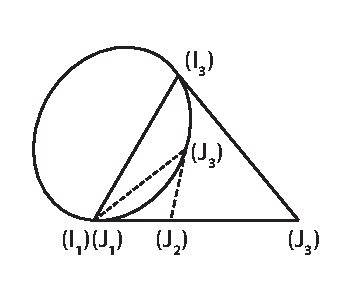
\includegraphics{cartangrp-f2}  
  \caption[]{\emph{Schemata of the plane at infinity}\\where the ombilical point and the points at infinity $(\mathbf{I}_{1})$, $(\mathbf{J}_{1})$, $\dots$,\\and the lines along the vectors $\ivec_{1}$, $\jvec_{1}$, $\dots$ are shown.}
\end{figure}

To express that the trihedral $\mathbf{A}\ivec_{1}\ivec_{2}\ivec_{3}$ is a right trihedral we use the equations \eqref{eq:2.3} and \eqref{eq:2.5} [theorem of \fsref{23}, p.~\pageref{sec:23}]. We obtain
\[
\beta^{2}=1,\qquad\alpha\gamma=1,\qquad\beta\mu+\lambda=0,\qquad\mu^{2}+2\rho=0,\qquad\alpha\beta\gamma=1.
\]

Then
\begin{equation}
  \label{eq:2.11}
  \left\{
    \begin{aligned}
      \ivec_{1}&=\alpha\jvec_{1},\\
      \ivec_{2}&=\jvec_{2}+\lambda\jvec_{1},\\
      \ivec_{3}&=\frac{1}{\alpha}\left[\jvec_{3}-\lambda\jvec_{2}-\frac{\lambda^{2}}{2}\jvec_{1}\right].
    \end{aligned}
  \right.
\end{equation}

The family of first order trihedrals therefore depends on the \emph{principal parameter} $t$, which characterises the position f the point $\mathbf{A}$ on the curve, as well as two secondary parameters $\alpha\neq 0$ and $\lambda$. The family of first order trihedrals is connected.

\somespace

\emph{Comparison of the infinitesimal displacement components of two first order trihedrals.} Suppose that the two trihedrals $\mathbf{A}\ivec_{1}\ivec_{2}\ivec_{3}$ and $\mathbf{A}\jvec_{1}\jvec_{2}\jvec_{3}$ varies while conserving the same apex. Let $\omega$ be the infinitesimal displacement components of the first trihedral, and $\bar\omega$ those of the second. We will calculate the components $\omega$ as functions of the components $\bar\omega$, $\lambda$, $\alpha$, $d\lambda$ and $d\alpha$. For this we use the formulae \eqref{eq:2.3}, \eqref{eq:2.7}, \eqref{eq:2.8} and \eqref{eq:2.11}:
\begin{align*}
  \omega_{1}=\ivec_{3}\times\overrightarrow{d\mathbf{A}}&=\frac{1}{\alpha}\left[\jvec_{3}-\lambda\jvec_{2}-\frac{\lambda^{2}}{2}\jvec_{1}\right]\times\overrightarrow{d\mathbf{A}}=\frac{1}{\alpha}\,\bar\omega_{1},\\
  \omega_{11}=\ivec_{3}\times{d\ivec_{1}}&=\frac{1}{\alpha}\left[\jvec_{3}-\lambda\jvec_{2}-\frac{\lambda^{2}}{2}\jvec_{1}\right][\alpha\,{d\jvec_{1}}+\jvec_{1}d\alpha]=\bar\omega_{11}-\lambda\bar\omega_{12}+\frac{d\alpha}{\alpha},\\
  \omega_{12}=\ivec_{2}\times{d\ivec_{1}}&=[\jvec_{2}+\lambda\jvec_{1}][\alpha\,d\jvec_{1}+\jvec_{1}d\alpha]=\alpha\bar\omega_{12},\\
  \omega_{21}=\ivec_{3}\times{d\ivec_{2}}&=\frac{1}{\alpha}\left[\jvec_{3}-\lambda\jvec_{2}-\frac{\lambda^{2}}{2}\jvec_{1}\right][d\jvec_{2}+\lambda\,d\jvec_{1}+\jvec_{1}d\lambda]\\
  &=\frac{1}{\alpha}\left[\bar\omega_{21}-\frac{\lambda^{2}}{2}\bar\omega_{12}+\lambda\bar\omega_{11}+d\lambda\right].
\end{align*}

In sum,
\begin{equation}
  \label{eq:2.12}
  \left\{
    \begin{aligned}
      \omega_{1}&=\frac{1}{\alpha}\bar\omega_{1},&&&\omega_{11}&=\bar\omega_{11}-\lambda\bar\omega_{12}+\frac{d\alpha}{\alpha},\\
      \omega_{12}&=\alpha\bar\omega_{12},&&&\omega_{21}&=\frac{1}{\alpha}\left[\bar\omega_{21}-\frac{\lambda^{2}}{2}\bar\omega_{12}+\lambda\bar\omega_{11}+d\lambda\right].
    \end{aligned}
  \right.
\end{equation}

Let us now focus on the linear combinations of the components of $\omega$ in which the differentials of the secondary parameters $d\alpha$, $d\lambda$ do not appear: these are linear combinations in $\omega_{1}$, $\omega_{2}$, $\omega_{3}$ and $\omega_{12}$, and their values depend uniquely on the choice of the trihedral $\mathbf{A}\ivec_{1}\ivec_{2}\ivec_{3}$ and the infinitesimal displacement of its apex. We call the following the \emph{principal components of order $1$}:
\[
\boxed{
\omega_{1},\quad\omega_{2}\text{ (which vanishes)},\quad\omega_{3}\text{ (which vanishes)},\quad\omega_{12}.
}
\]
\somespace

\emph{Remark.} We could have seen these are the principal components: their linear combinations are linear combinations of the forms $\omega$ which vanishes when $dt$ vanishes. The hypothesis $t=0$ implies that $\overrightarrow{d\mathbf{A}}=0$ and $d\ivec_{i}$ is parallel to $\ivec_{i}$, from which $\omega_{1}=\omega_{2}=\omega_{3}=0$, $\omega_{12}=0$. The components $\omega_{1}$, $\omega_{2}$, $\omega_{3}$, $\omega_{12}$ are therefore the principal components. There are no others, since the number of principal components is the number of components of $\omega$ minus the number of secondary parameters, $6-2=4$.

\paragraph{Second order trihedrals.}
\label{sec:28}
According to the formulae \eqref{eq:2.12} every point $\mathbf{A}$ on the curve possesses a first order trihedral such that
\begin{equation}
  \label{eq:2.13}
  \omega_{1}=\omega_{12}.
\end{equation}

We will call these the second order trihedrals.

This definitions fails when $\bar\omega_{12}=0$, in which case the component $\omega_{12}$ is zero for all first order trihedrals. Then it becomes impossible to distinguish among the first order trihedrals with the help of the relations relative to the principal components. We will examine this exceptional case in more details in paragraph \fsref{30} (p.~\pageref{sec:30}).

\somespace

\emph{Comparisons of two second order trihedrals.} Now denote a particular second order trihedral by $\mathbf{A}\jvec_{1}\jvec_{2}\jvec_{3}$ and $\mathbf{A}\ivec_{1}\ivec_{2}\ivec_{3}$ the most general second order trihedral. The formulae \eqref{eq:2.12} tell us that in the equations \eqref{eq:2.11} $\lambda$ is arbitrary, but
\begin{equation}
  \label{eq:2.14}
  \alpha=\pm1.
\end{equation}

The families of second order trihedrals therefore decompose into two sub-families containing no common element.

By an arbitrary procedure we distinguish one of these two sub-families. This operation will be called \emph{orientating} of the curve, analogous to the case of real curves: the family of first order trihedrals attached at a non-oriented real curve is disconnected and decomposes into two connected sub-families, and choosing one of these sub-families amounts to orientating the curve. Similarly, we call only the distinguished sub-family of the second order trihedrals attached to our minimal curve oriented.

According to \eqref{eq:2.11} and \eqref{eq:2.12}, if $\mathbf{A}\jvec_{1}\jvec_{2}\jvec_{3}$ and $\mathbf{A}\ivec_{1}\ivec_{2}\ivec_{3}$ are two second order trihedrals of an oriented curve,
\begin{align}
  \label{eq:2.15}
  &\left\{
    \begin{aligned}
      \ivec_{1}&=\jvec_{1},\\
      \ivec_{2}&=\jvec_{2}+\lambda\jvec_{1},\\
      \ivec_{3}&=\jvec_{3}-\lambda\jvec_{2}-\frac{\lambda^{2}}{2}\jvec_{1};
    \end{aligned}
  \right.
\\
  \label{eq:2.16}
  &\left\{
    \begin{aligned}
      \omega_{1}&=\bar\omega_{1},\\
      \omega_{11}&=\bar\omega_{11}-\lambda\bar\omega_{1},\\
      \omega_{21}&=\bar\omega_{21}-\frac{\lambda^{2}}{2}\bar\omega_{1}+\lambda\bar\omega_{11}+d\lambda,
    \end{aligned}
  \right.
\end{align}
$\lambda$ being arbitrary.

The relations \eqref{eq:2.11} and \eqref{eq:2.12} also shows that to every second order $\mathbf{A}\jvec_{1}\jvec_{2}\jvec_{3}$ on a oriented curve there corresponds a second order trihedral $\mathbf{A}\ivec_{1}\ivec_{2}\ivec_{3}$ on the curve oriented in the opposite sense such that we have
\begin{align}
  \label{eq:2.17}
  &\left\{
    \begin{aligned}
      \ivec_{1}&=-\jvec_{1},\\
      \ivec_{2}&=\hphantom{+}\jvec_{2},\\
      \ivec_{3}&=-\jvec_{3};
    \end{aligned}
  \right.
  \\
  \label{eq:2.18}
  &\left\{
    \begin{aligned}
      \omega_{1}&=-\bar\omega_{1},\\
      \omega_{11}&=\hphantom{+}\bar\omega_{11},\\
      \omega_{21}&=-\bar\omega_{21}.
    \end{aligned}
  \right.
\end{align}

According to \eqref{eq:2.16} the component $\omega_{1}$ is the same for all second order trihedrals of an oriented curve, and this is a Pfaffian form depending only on the principal parameter and its constitutes a \emph{second order differential invariant}. We will call it the differential of the \emph{pseudo-arc} and we denote it by $d\sigma$ [c.f.~the end of \fsref{18}, p.~\pageref{sec:18}]. The first formula \eqref{eq:2.18} shows that $d\sigma$ transforms into its opposite when we change the orientation of the curve.

The linear combinations of an second order frame where $d\lambda$ does not appear are the linear combinations of the following \emph{principal components}:
\begin{center}  
\begin{tabular}{|c|c|}
  \hline
  Order $1$&Order $2$\\
  \hline
  $\omega_{1},\quad\omega_{2}(=0),\quad\omega_{3}(=0),\quad\omega_{12}(=\omega_{1})$&$\omega_{11}$\\
  \hline
\end{tabular}
\end{center}

We could have seen this: the second order frame depend on \emph{one} less secondary parameter than the first order frames. The linear combinations of $\omega$ where the differentials of the second order parameters do not appear therefore must be the linear combinations of \emph{one} principal component at most. The hypothesis $dt=0$ entails, according to \eqref{eq:2.15}, $d\ivec_{1}=0$ and therefore, according to \eqref{eq:2.7}, $\omega_{11}=0$. The second order principal component is therefore $\omega_{11}$.

\paragraph{Third order trihedrals.}
\label{sec:29}
We distinguish in the family of second trihedrals those special trihedrals which we will call third order trihedrals, those which are distinguished by a condition for the third order principal component, which is
\begin{equation}
  \label{eq:2.19}
  \omega_{11}=0.
\end{equation}

Every oriented curve has a unique third order trihedral at each of its point, $\mathbf{A}\ivec_{1}\ivec_{2}\ivec_{3}$. According to \eqref{eq:2.18} its mirror image with respect to $\ivec_{2}$, $\mathbf{A}\jvec_{1}\jvec_{2}\jvec_{3}$ defined by \eqref{eq:2.17} is a third order trihedral of the curve oriented in the opposite sense.

We set $\omega_{21}=k\,d\sigma$. We call the quantity $k$ curvature, or fourth order invariant \footnote{The name invariant signifies that $k$ does not vary when the curve undergoes a displacement.}.

According to \eqref{eq:2.18} the value of the curvature is independent of the orientation. We obtain formulae analogous to the \emph{Frenet formulae} (\fsref{10}, p.~\pageref{sec:10}):
\begin{equation}
  \label{eq:2.20}
  \left\{
    \begin{aligned}
      \overrightarrow{d\mathbf{A}}&=d\sigma\,\ivec_{1},&&&d\ivec_{2}&=d\sigma(k\ivec_{1}-\ivec_{3}),\\
      d\ivec_{1}&=d\sigma\,\ivec_{2},&&&d\ivec_{3}&=-k\,d\sigma\,\ivec_{2}.
    \end{aligned}
  \right.
\end{equation}

\emph{Structure theorem.} Let us specify a function $k(\sigma)$ arbitrarily. According to the structure theorem stated in paragraph \fsref{25} (p.~\pageref{sec:25}), there exists a cyclic trihedral $\mathbf{A}\ivec_{1}\ivec_{2}\ivec_{3}$ depending on the parameter $\sigma$ such that the equations \eqref{eq:2.20} hold. The first of these equations shows that the apex $\mathbf{A}$ describes a minimal curve $C$. Moreover, $\omega_{2}=\omega_{3}=0$, therefore the trihedral is a first order trihedral of $C$; $\omega_{1}=\omega_{12}$, and hence the trihedral is second order; $\omega_{11}=0$, and hence the trihedral is a third order trihedral for $C$, suitably oriented, and the curvature of $C$ is $k(\sigma)$ at the point with the pseudo-arc $\sigma$. Hence the structure theorem: \emph{Along a minimal curve the curvature is an arbitrary function of the pseudo-arc.}

\paragraph{Exceptional case.}
\label{sec:30}
The preceding definitions fail for \emph{the curves whose components $\omega_{12}$ of the first order trihedral are constantly zero} \footnote{Similarly the family of real curves contains the exceptional category of straight lines, for which we cannot attach Frenet trihedrals.}.

For these trihedrals there then exists only one principal component $\omega_{1}$, and the preceding, which consists of defining the second order trihedral by the relations among the principal components of the first order trihedral is inapplicable.

Let us consider two such curves $C$ and $C\str$. Let $\mathbf{T}$ be the family of first order trihedrals on $C$, $\mathbf{T}\str$ the family on $C\str$. $\mathbf{T}$ is a one-parameter family, and we can associated at the moving trihedral $\mathbf{T}$ a moving trihedral $\mathbf{T}\str$ whose infinitesimal displacement has the same components such that to a particular trihedral $\mathbf{T}_{0}$ there corresponds an arbitrarily chosen trihedral $\mathbf{T}\str_{0}$: for this it suffices to integrate the equations
\[
\omega_{1}=\omega\str_{1},\qquad\omega_{11}=\omega\str_{11},\qquad\omega_{21}=\omega_{21}\str,
\]
which constitute a system of three differential equations in three unknown functions, the initial values being fixed. Then the displacement superimposing the arbitrary first order trihedral $\mathbf{T}_{0}$ and $\mathbf{T}\str_{0}$ of $C$ and $C\str$ superimpose these two curves (see the \emph{fundamental condition of equality}, \fsref{26}, p.~\pageref{sec:26}).

In particular a three parameter family of displacement permits us to transform the curve $C$ into itself: every displacement transforming one of the first order trihedral of $C$ to any other leaves the curve fixed. This shows that no first order trihedral has intrinsic special property: hence the failure of the procedure that we used to define the second order trihedrals.

On the other hand the curves under consideration are very simple: the relation $\omega_{12}=0$ entails $d\ivec_{1}=\omega_{11}\ivec_{1}$, and the tangent remains fixed along the curve parallel to a fixed direction, and hence these curves are isotropic lines \footnote{The family of displacement transforming a non-isotropic line into itself depends on two parameters, is disconnected and consists of two connected sub-families. However, we have just seen that the family of displacements transforming one isotropic line to itself depends on three parameters and is connected.}.


\section{Problems of equality and contact}
\label{sec:probl-equal-cont}

\paragraph{Equality problem.}
\label{sec:31}
The definitions that we have given in the course of the preceding section are such that if we subject our minimal curve to an arbitrary displacement, the elements $k$ and $d\sigma$ do not change and the first, second and third order trihedrals are transformed by the same displacement: this gives the intrinsic significance of the components $\omega$ [c.f.~\fsref{26}, p.~\pageref{sec:26}].

In particular, the problem of \emph{determining the displacements which superimpose two given oriented minimal curves $C$ and $C\str$} is equivalent to the problem of finding the displacements which superimpose the third order trihedrals $C$ and $C\str$. The fundamental condition for equality (\fsref{26}, p.~\pageref{sec:26}) makes the problem into searching all bijective correspondances that can be established between $C$ and $C\str$ satisfying the equations
\begin{equation}
  \label{eq:2.21}
  k(\sigma)=k\str(\sigma\str),\qquad d\sigma=d\sigma\str.
\end{equation}

If the equality problem is posed for two non-oriented curves $C$ and $C\str$, we must construct, other than the preceding correspondences, those that satisfy the equations
\begin{equation}
  \label{eq:2.22}
  k(\sigma)=k\str(\sigma\str),\qquad d\sigma=-d\sigma\str.
\end{equation}
Each of the correspondences obtained will furnish one of the displacement superimposing $C$ and $C\str$.

Let us examine the \emph{special case} where one of the curvature is constant. The other curvature must have the same constant, otherwise the problem of superimposing the curves is unsolvable. The correspondances \eqref{eq:2.21} and \eqref{eq:2.22} each depends on one arbitrary parameter, and hence we can superimpose $C$ and $C\str$ by making the two coincident at two of their arbitrarily given points, in the same or opposite orientation. In particular, the curve $C$ can slide on itself (as a helix), and if $C_{1}$ is the curve obtained by changing the orientation of $C$, displacements would permit us to superimpose $C$ and $C_{1}$.

\paragraph{Contact problem of order 1.}
\label{sec:32}
This problem can be solved immediately: consider two minimal curves $C$ and $C\str$ and two of their points $\mathbf{A}_{0}$ and $\mathbf{A}_{0}\str$. The displacements superimposing $C$ and $C\str$ and realising a contact of order $\ge 1$ there are those that makes an arbitrarily chosen first order trihedral $\mathbf{T}\str_{0}$ at $\mathbf{A}\str_{0}$ coincident with the different first order trihedrals $\mathbf{T}_{0}$ attached at $\mathbf{A}_{0}$. These displacements therefore depend on two parameters.

On the other hand, we have determined that a first order contact element is determined by the data of the associated family of first order trihedrals and \emph{vice versa}.

We will solve \emph{the contact problems of order greater than one} by equivalence, by applying the stated contact condition in paragraph \fsref{16} (p.~\pageref{sec:16}). This condition amounts to no longer defining the difference between two points in terms of their distance, but, for example, in terms of the greatest absolute value of the difference of their coordinates.

\paragraph{Contact problem of order 2.}
\label{sec:33}
Consider a displacement solving the first order contact problem: it superimposes any first order trihedral $\mathbf{T}\str_{0}$ attached at $\mathbf{A}\str_{0}$ to a first order trihedral $\mathbf{T}_{0}$ attached at $\mathbf{A}_{0}$. For the displacement to realise a contact of order $\ge 2$, it is necessary and sufficient that we can find an infinitesimal displacement of first order trihedral $\mathbf{T}_{0}$ and an infinitesimal displacement of the trihedral $\mathbf{T}\str_{0}$ which are equal and which displace the origin of these trihedrals. This condition translates into a system of linear equations in terms of the differentials of the parameters
\begin{equation}
  \label{eq:2.23}
  \omega_{1}=\omega_{1}\str,\qquad\omega_{11}=\omega_{11}\str,\qquad\omega_{12}=\omega_{12}\str,\qquad\omega_{21}=\omega_{21}\str,
\end{equation}
this system must admit a solution which does not annihilate the differentials of the principal parameters.

Suppose that we have chosen a second order trihedral $\mathbf{T}_{0}\str$: $\omega_{1}\str=\omega_{12}\str$. We must have $\omega_{1}=\omega_{12}$: $\mathbf{T}_{0}$ must equally be a second order trihedral. If this is the case then the solution we are searching for of the system \eqref{eq:2.23} surely exists: since $\omega_{1}$, $\omega_{11}$ and $\omega_{21}$ are linear independent forms in the differentials of the principal parameters and the two secondary parameters [c.f.~\fsref{27}, p.~\pageref{sec:31}].

The the solutions of second order contact problem are the displacements that superimpose a second order trihedral of $\mathbf{A}\str_{0}$ with the different second order trihedrals of $\mathbf{A}_{0}$.

The second order contact problem is therefore determined by the families of second order trihedrals and \emph{vice versa}. Similarly $d\sigma^{2}$ is determined by the data of the second order contact element and the differential of one of the coordinates $x$, $y$ and $z$.

Henceforth we will assume the two curves $C$ and $C\str$ to be oriented and we consider a second order contact to be established between the two curves only when the second order trihedral of the \emph{oriented} curve $C$ coincide with a second order trihedral of the \emph{oriented} curve $C\str$.


\paragraph{Contact problem of order 3.}
\label{sec:34}
Consider a contact of order $\ge 2$ established at a point $\mathbf{A}_{0}$ between two oriented minimal curves $C$ and $C\str$: every second order trihedral $\mathbf{T}\str_{0}$ of $C\str$ having its apex at $\mathbf{A}_{0}$ coincides with a second order trihedral $\mathbf{T}_{0}$ of $C$ with apex $\mathbf{A}_{0}$. For the contact to realise a contact of order $\ge 3$, it is necessary and sufficient that we can find two equal infinitesimal displacements of these second order trihedrals. The condition easily leads to the following form: there must exist between the differentials of the principal parameters of the two curves a relation realising the equality of the principal components
\[
\omega_{1}=\omega_{1}\str,\qquad\omega_{11}=\omega_{11}\str.
\]

Let us choose a third order trihedral $\mathbf{T}\str_{0}$ of $C$: $\omega_{11}\str=0$. We must have $\omega_{11}=0$, $\mathbf{T}_{0}$ must be the third order trihedral of ${C}$, and the correspondence to be established between the differentials of the principal parameters is defined by $\omega_{1}=\omega_{1}\str$ and it always exists.

The solution of the third order contact problem is therefore the displacements that superimpose the third order trihedrals of the given curves.

The third order contact element is determined by the third order trihedral and \emph{vice versa}.

\paragraph{Contact problems of order $>3$.}
\label{sec:35}
Consider a contact of order $\ge 3$ established at a point $\mathbf{A}_{0}$ between two oriented curves $C$ and $C\str$. Their third order trihedrals coincide. For the contact to be of order $\ge 4$, it is necessary and sufficient that we can find two equal infinitesimal displacements of these two trihedrals: this condition is equivalent to the equality $k=k\str$.

Suppose $k=k\str$. For the contact to be of order $\ge 5$, it is necessary and sufficient that we can find two infinitesimal displacements of these two trihedrals satisfying the relation $dk=dk\str$. This condition is equivalent to $\dfrac{dk}{d\sigma}=\dfrac{dk\str}{d\sigma\str}$, etc. From this we have the following theorem:

\somespace

For the solution of the \emph{contact problem of order $P\ge 4$} of two points $\mathbf{A}_{0}$ and $\mathbf{A}_{0}\str$ of two oriented minimal curves $C$ and $C\str$, the solvability condition is that we have, at these points,
\[
k=k\str,\qquad \frac{dk}{d\sigma}=\frac{dk\str}{d\sigma\str},\qquad\dots,\qquad\frac{d^{P-1}k}{d\sigma^{P-1}}=\frac{d^{P-1}k\str}{d\sigma^{\star P-1}}.
\]
When these relations are satisfied the problem admits a single solution: the displacement which superimposes the third order trihedrals of the points $\mathbf{A}_{0}$ and $\mathbf{A}\str_{0}$.


\section{Complements}
\label{sec:complements}

To practically solve the equality and contact problems, we need to know how to effectively determine the various order trihedrals and the invariant $k$. We are going to show how we can achieve this aim in two ways: by calculating them and by the construction of infinitesimal geometry.

\paragraph{Analytic determination of the trihedrals of various order, of $k$ and of $d\sigma$.}
\label{sec:36}
Consider a minimal curve traced by a point $(x,y,z)$, the reference trihedral used being tri-rectangular. We have
\[
dx^{2}+dy^{2}+dz^{2}=0.
\]
Therefore there exists a parameter $t$ such that
\[
\frac{2dx}{1-t^{2}}=\frac{2dy}{i(1+t^{2})}=\frac{dz}{t}.
\]
Let $f(t)$ be the common value of these fractions. We have
\label{x:weierstrass}
\begin{align*}
  x(t)&=\int_{t_{0}}^{t}\frac{1-t^{2}}{2}f(t)dt+x_{0},\\
  y(t)&=\int_{t_{0}}^{t}i\frac{1+t^{2}}{2}f(t)dt+y_{0},\\
  z(t)&=\int_{t_{0}}^{t}tf(t)dt+z_{0}.
\end{align*}
These formulae, called \emph{Weierstrass's formulae}, furnish the parametric representation of the most general minimal curve.

We say that the following trihedral $\mathbf{A}\jvec_{1}\jvec_{2}\jvec_{3}$ is a particular first order trihedral:
\[
\begin{matrix}
  \jvec_{1}&\text{has components:}&\dfrac{1-t^{2}}{2},&i\dfrac{1+t^{2}}{2},&t,\\
  \jvec_{2}&\text{has components:}&-t,&it,&1,\\
  \jvec_{3}&\text{has components:}&1,&-i,&0.
\end{matrix}
\]

Indeed, $\jvec_{1}$ is just the tangent and we have
\begin{gather*}
  \jvec_{1}{}^{2}=0,\qquad\jvec_{2}{}^{2}=1,\qquad\jvec_{3}^{2}=0,\qquad \jvec_{1}\times\jvec_{2}=0,\\
  \jvec_{2}\times\jvec_{3}=0,\qquad\jvec_{1}\times\jvec_{3}=0,\qquad(\jvec_{1}\wedge\jvec_{2})\times\jvec_{3}=i.
\end{gather*}
Formulae \eqref{eq:2.8} permit use to calculate the components $\bar\omega$ of the infinitesimal displacement of this trihedral:
\begin{align*}
  \bar\omega_{1}&=\jvec_{3}\times\overrightarrow{d\mathbf{A}}=f(t)dt,&\bar\omega_{11}&=\jvec_{3}\times d\jvec_{1}=0,\\
  \bar\omega_{12}&=\jvec_{2}\times d\jvec_{1}=dt,&\bar\omega_{21}&=\jvec_{3}\times d\jvec_{2}=0.
\end{align*}

The most general first order trihedral is defined by the formulae \eqref{eq:2.11} in paragraph \fsref{27} (p.~\pageref{eq:2.11}), and the formulae \eqref{eq:2.12} of paragraph \fsref{27} takes the form
\begin{equation}
  \label{eq:2.24}
  \left\{
    \begin{aligned}
      \omega_{1}&=\frac{1}{\alpha}f(t)dt,&\omega_{11}&=-\lambda\,dt+\frac{d\alpha}{\alpha},\\
      \omega_{12}&=\alpha\,dt,&\omega_{21}&=\frac{1}{\alpha}\left(-\frac{\lambda^{2}}{2}dt+d\lambda\right).
    \end{aligned}
  \right.
\end{equation}

The second order trihedrals are defined by the condition $\omega_{1}=\omega_{12}$ which is equivalent to $\alpha=\sqrt{f}$. The third order trihedrals are defined by the condition $\omega_{1}=\omega_{12}$, $\omega_{11}=0$, which is equivalent to
\[
\alpha=\sqrt{f},\quad\lambda=\frac{1}{2}\frac{f'}{f}.
\]
Then, for these third order trihedrals,
\[
\omega_{1}=d\sigma,\qquad\omega_{21}=k\,d\sigma,
\]
we have
\begin{equation}
  \label{eq:2.25}
  d\sigma=\sqrt{f}\,dt,\qquad k=\frac{1}{f}\left[\frac{1}{2}\frac{f''}{f}-\frac{5}{8}\frac{f'^{2}}{f^{2}}\right].
\end{equation}

\somespace

\emph{Application.} Let us determine the constant curvature minimal curves. According to \eqref{eq:2.25} the problem consists of integrating the equation
\[
\frac{1}{f}\left[\frac{1}{2}\frac{f''}{f}-\frac{5}{8}\frac{f'^{2}}{f^{2}}\right]=\text{constant.}
\]

Let us search a particular solution of the form $f=at^{m}$.

We obtain
\[
k=\frac{1}{at^{m+2}}\left[\frac{1}{2}m(m-1)-\frac{5}{8}m^{2}\right].
\]

If $k=0$ then we can take $m=-4$. Otherwise we need to take
\[
m=-2\qquad\text{and}\qquad a=\frac{1}{2k}.
\]

We learned in paragraph \fsref{31} (p.~\pageref{sec:31}) that the set of curves with given constant curvature can be deduced by the particular curves thus obtained by applying the most general displacement.

We are going to determine by a second, more geometric procedure the curves in question.

\paragraph{Applications of the ``Frenet formulae'' \eqref{eq:2.20} to the search of the curves with constant curvature.}
\label{sec:37}
First suppose that $k=0$. We have $d\ivec_{3}=0$, and therefore $\ivec_{3}$ is a constant vector, let us call it $\kvec_{3}$. The equation
\[
\d\ivec_{2}=-\ivec_{3}d\sigma
\]
gives
\[
\ivec_{2}=-\sigma\kvec_{3}+\kvec_{2},
\]
$\kvec_{2}$ being a new constant vector. The equation
\[
d\ivec_{1}=\ivec_{2}d\sigma\qquad\text{gives}\qquad\ivec_{1}=-\frac{1}{2}\sigma^{2}\kvec_{3}+\sigma\kvec_{2}+\kvec_{1},
\]
$\kvec_{1}$ being a third constant vector. Hence, $\mathbf{A}_{0}$ denoting a fixed point,
\[
\overrightarrow{\mathbf{A}_{0}\mathbf{A}}=-\frac{1}{6}\sigma^{3}\kvec_{3}+\frac{1}{2}\sigma^{2}\kvec_{2}+\sigma\kvec_{1}.
\]

We obtain a \emph{space cubic} osculating to the plane at infinity at a point of the ombilical conic.

Now suppose that $k$ is constant but non-zero. According to formulae \eqref{eq:2.20}, we have
\[
d\left(\ivec_{1}+\frac{1}{k}\ivec_{3}\right)=0,
\]
therefore
\[
\ivec_{1}+\frac{1}{k}\ivec_{3}
\]
is a constant vector (of length $\sqrt{2/k}$). With this result, let us introduce a point $\mathbf{M}$ defined by the relation
\[
\overrightarrow{\mathbf{AM}}=R\ivec_{2},
\]
where $R$ is a constant length. We have
\[
\overrightarrow{d\mathbf{M}}=\overrightarrow{d\mathbf{A}}+R\,d\ivec_{2}=[(1+kR)\ivec_{1}-R\ivec_{3}]d\sigma.
\]
Let use take
\[
R=-\frac{1}{2k},
\]
it becomes
\[
\overrightarrow{d\mathbf{M}}=\frac{1}{2}\left[\ivec_{1}+\frac{1}{k}\ivec_{3}\right]d\sigma.
\]
The vector $\dfrac{\overrightarrow{d\mathbf{M}}}{d\sigma}$ is a fixed vector: the point $\mathbf{M}$ describes a curve $\Delta$ parallel to the vector $\ivec_{1}+\dfrac{1}{k}\ivec_{3}$. $\Delta$ is not an isotropic line, it is perpendicular to $\ivec_{2}$, and therefore $\mathbf{A}$ remains on the cylinder with axis $\Delta$ and radius $R$. Then \emph{the curves with non-zero constant curvature are the minimal circular helices}.

Given such a helix and one of its points $\mathbf{A}$, the two third order trihedrals $\mathbf{A}\ivec_{1}\ivec_{2}\ivec_{3}$, the curvature $k$ and the pseudo-arc $\sigma$ are easy to determine. Let $\mathbf{AM}$ be the normal to the cylinder at $\mathbf{A}$, $\mathbf{M}$ being its point of contact with the axis. This line carries two unit vectors, of the two, $\ivec_{2}$ is characterised by the following property: all of the right cyclic trihedrals having $\ivec_{2}$ as the second vector have their first vectors along one of the isotropic curves in the tangent plane to the cylinder at $\mathbf{A}$, and these isotropic lines must be tangent to the minimal helix. We therefore set
\[
\overrightarrow{\mathbf{AM}}=R\ivec_{2},
\]
and we have
\[
k=-\frac{1}{2R}.
\]
$\ivec_{1}$ and $\ivec_{3}$ are determined up to multiples of $\pm 1$ by the requirement that the vector $\ivec_{1}+\dfrac{1}{k}\ivec_{3}$ have its support on the generatrix of the cylinder.
Finally, the relation
\[
\overrightarrow{d\mathbf{M}}=\frac{1}{2}\left(\ivec_{1}+\frac{1}{k}\ivec_{3}\right)d\sigma
\]
gives us the pseudo-arc element.


\paragraph{Geometric interpretation of $k$.}
\label{sec:38}
There exists one and only one oriented minimal circular helix which has a contact of order $4$ with the given oriented minimal curve at a given point on the curve: this is the helix having the same curvature and third order trihedral as the curve at this point. The helix corresponding to the opposite direction is manifestly the same helix oriented in the opposite sense. This helix is therefore attached geometrically at this point of the curve, independent of orientation (an exceptional case needs to be noted: the case where the cuve has vanishing curvature, and there no minimal helix can realise a fourth order contact with the curve, but such a contact can be obtained with a minimal cubic with zero curvature).

We then obtain a geometrical interpretation of $k$: it is the curvature of this helix.

Similarly, the arc element of the curve is an infinitesimal quantity equivalent to the arc element of the helix, the two third order trihedrals of the curve are also those of the helix. We are going to find for the elements of order $<$ another geometric interpretation without using this helix, which is a function of the fourth order contact element.

For this, we ar going to study the properties of the minimal curve at a neighbourhood of one of its points $\mathbf{A}$.


\paragraph{Reduced equations.}
\label{sec:39}
We can, as we have done in paragraph \fsref{21a}\textit{bis.}, try to find the reduced equations of the curve in a neighbourhood of one of its pints $\mathbf{A}$ directly and derive from these the Frenet formulae. Let us follow the procedure in reverse here. Let
\begin{align*}
  y&=f(x,\sigma)=P_{1}(x,\sigma)+P_{2}(x,\sigma)+\dots+P_{n}(x,\sigma)+\cdots,\\
  z&=\phi(x,\sigma)=Q_{1}(x,\sigma)+Q_{2}(x,\sigma)+\dots+Q_{n}(x,\sigma)+\cdots,
\end{align*}
be the equations of the curve with respect to the right cyclic trihedral attached at the point $\mathbf{A}$, $P_{i}(x,\sigma)$ and $Q_{i}(x,\sigma)$ denoting homogeneous polynomials of degree $i$ in $x$ whose coefficients depend on the curvilinear abscissa $\sigma$ of the point $\mathbf{A}$. Let us take a fixed point $\mathbf{B}$ of coordinates $x$, $y$, $z$ with respect to the cyclic trihedral of origin $\mathbf{A}$ on the curve. By expressing that the point of the \emph{moving} coordinates $(x,y,z)$ is \emph{fixed}, we obtain, according to the Frenet formulae \eqref{eq:2.20} (p.~\pageref{eq:2.20}), the relations
\begin{alignat*}{3}
  &\frac{dx}{d\sigma}+1+ky&{}={}0,\\
  &\frac{dy}{d\sigma}+x-kz&{}={}0,\\
  &\frac{dz}{d\sigma}-y&{}={}0.
\end{alignat*}
From this, it follows the relations
\begin{alignat*}{3}
  &-\frac{\pd f}{\pd x}(1+kf)+\frac{\pd f}{\pd\sigma}+x-k\phi&{}=0,\\
  &-\frac{\pd \phi}{\pd x}(1+kf)+\frac{\pd \phi}{\pd\sigma}-f&{}=0.  
\end{alignat*}

There relations must hold regardless of the point $\mathbf{A}$ and the fixed point $\mathbf{B}$, and therefore are identities in $x$ and $\sigma$. By equating the independent terms of $x$ and the coefficients of different powers of $x$ on the left hand sides, we obtain successively
\begin{align*}
  P_{1}&=0,&Q_{1}&=0,\\
  P_{2}&=\frac{1}{2}x^{2},&Q_{2}&=0,\\
  P_{3}&=0,&Q_{3}&=-\frac{1}{6}x^{3},\\
  P_{4}&=-\frac{1}{12}kx^{4},&Q_{4}&=0,\\
  P_{5}&=-\frac{1}{60}\frac{dk}{d\sigma}x^{5},&Q_{5}&=\frac{1}{15}kx^{5}.
\end{align*}
The reduced equations of the curve are therefore
\begin{equation}
  \label{eq:2.26}
  \left\{
    \begin{aligned}
      y&=\hphantom{+}\frac{1}{2}x^{2}-\frac{1}{12}kx^{4}-\frac{1}{60}\frac{dk}{d\sigma}x^{5}+\cdots,\\
      z&=-\frac{1}{6}x^{3}+\frac{1}{15}kx^{5}+\cdots
    \end{aligned}
  \right.
\end{equation}
We can restrict our calculation to $y$ only, since we have
\[
dy^{2}+2dx\,dz=0,
\]
from which
\[
\frac{dz}{dx}=-\frac{1}{2}\left(\frac{dy}{dx}\right)^{2}.
\]

\paragraph{Geometric constructions of pseudo-arc.}
\label{sec:40}
\emph{a.} The abscissa $x$ of a point $\mathbf{A}'$ infinitesimally close to $\mathbf{A}$ gives the pseudo-arc $\sigma$ of $\Delta'$ when we take $\mathbf{A}$ as the origin. The square of the distance $\mathbf{AA}'=c$ is
\begin{equation}
  \label{eq:2.27}
  c^{2}=y^{2}+2xz\sim \frac{1}{4}x^{4}-\frac{1}{3}x^{4}\sim-\frac{1}{12}x^{4}\sim-\frac{1}{12}d\sigma^{4},
\end{equation}
\emph{$d\sigma^{4}$ is therefore an infinitesimally small quantity equivalent to $-12c^{2}$}.

This formula gives four values to $d\sigma$ corresponding to the two possible orientations and the two possible definitions of the right cyclic trihedrals as in paragraph \fsref{23} (p.~\pageref{sec:23}). However we want a geometrical interpretation which gives us only two values of $d\sigma$, corresponding to the two orientations of the curve.

\somespace

\emph{b.} For this, let us choose arbitrarily a direction $\mathbf{D}$ not lying in the normal and osculating plane $\mathbf{A}\ivec_{1}\ivec_{2}$, and a direction $\mathbf{D}'$ in the place which is not parallel to the tangent at $\mathbf{A}$. Let us consider the parallelepiped having the diagonal $\mathbf{AA}'$ whose edges are parallel to the tangent at $\mathbf{A}$, $\mathbf{D}'$ and $\mathbf{D}$. if we modify the choice of $\mathbf{D}$ and $\mathbf{D}'$ we obtain other parallelepipeds, but their (oriented) volumes are the same infinitesimally small quantities $v$. Let us calculate $v$ by making the following particular choice: $\mathbf{D}$ is parallel to $\ivec_{3}$ and $\mathbf{D}'$ is parallel to $\ivec_{2}$. The formulae \eqref{eq:2.26} (\fsref{39}, p.~\pageref{eq:2.26}) and \eqref{eq:2.5} (\fsref{23}, p.~\pageref{eq:2.5}) give
\[
v=-\frac{i}{12}x^{6}+\dots\sim-\frac{i}{12}d\sigma^{6}.
\]

We then obtain, besides \eqref{eq:2.27}, the formula
\begin{equation}
  \label{eq:2.28}
  d\sigma^{6}=12iv,
\end{equation}
which gives a second geometric interpretation of $d\sigma$.

\somespace

\emph{c.} Only by dividing \eqref{eq:2.27} and \eqref{eq:2.28} do we obtain a rational expression of $d\sigma^{2}$
\begin{equation}
  \label{eq:2.29}
  d\sigma^{2}=-\frac{iv}{c^{2}}.
\end{equation}

Let us show how this formula permits us to determine $d\sigma$ when we know the rectangular coordinates of the parametric equations of the curve $x(t)$, $y(t)$, $z(t)$. We have
\[
\overrightarrow{\mathbf{AA}'}=\frac{\overrightarrow{d\mathbf{A}}}{dt}dt+\frac{1}{2}\frac{d^{2}\mathbf{A}}{dt^{2}}(dt)^{2}+\frac{1}{6}\frac{\overrightarrow{d^{3}\mathbf{A}}}{dt^{3}}(dt)^{3}+\cdots
\]
Take $\mathbf{D}'$ to be the direction of $\dfrac{\overrightarrow{d^{2}\mathbf{A}}}{dt^{2}}$, $\mathbf{D}$ the direction of $\dfrac{\overrightarrow{d^{3}\mathbf{A}}}{dt^{3}}$. It becomes
\[
v=\frac{1}{12}V(dt)^{6},
\]
$V$ being the volume of the parallelepiped with edges
\[
\frac{\overrightarrow{d\mathbf{A}}}{dt},\qquad
\frac{\overrightarrow{d^{2}\mathbf{A}}}{dt^{2}},\qquad
\frac{\overrightarrow{d^{3}\mathbf{A}}}{dt^{3}},
\]
i.e.,
\[
V=
\begin{vmatrix}
  x'&y'&z'\\
  x''&y''&z''\\
  x'''&y'''&z'''
\end{vmatrix}.
\]
On the other hand, $c^{2}$ is an infinitesimally small quantity equivalent to
\[
\biggl(\frac{\overrightarrow{d\mathbf{A}}}{dt}dt+\frac{1}{2}\frac{\overrightarrow{d^{2}\mathbf{A}}}{dt^{2}}dt^{2}+\frac{1}{6}\frac{\overrightarrow{d^{3}\mathbf{A}}}{dt^{3}}dt^{3}\biggr)^{2}.
\]

But
\[
\biggl(\frac{\overrightarrow{d\mathbf{A}}}{dt}\biggr)^{2}=0,
\]
from which
\[
\frac{\overrightarrow{d\mathbf{A}}}{dt}\times\frac{\overrightarrow{d^{2}\mathbf{A}}}{dt^{2}}=0,\qquad\biggl(\frac{\overrightarrow{d^{2}\mathbf{A}}}{dt^{2}}\biggr)^{2}+\frac{\overrightarrow{d\mathbf{A}}}{dt}\times\frac{\overrightarrow{d^{3}\mathbf{A}}}{dt^{3}}=0,
\]
and
\[
c^{4}=\frac{1}{4}\biggl(\frac{\overrightarrow{d^{2}\mathbf{A}}}{dt^{2}}\biggr)^{2}dt^{4}+\frac{1}{3}\frac{\overrightarrow{d\mathbf{A}}}{dt}\times\frac{\overrightarrow{d^{3}\mathbf{A}}}{dt^{3}}dt^{4}+\dots=-\frac{1}{12}\biggl(\frac{\overrightarrow{d^{2}\mathbf{A}}}{dt^{2}}\biggr)^{2}dt^{4}+\cdots
\]
The formula \eqref{eq:2.29} therefore gives
\[
d\sigma^{2}=+i\frac{
  \begin{vmatrix}
  x'&y'&z'\\
  x''&y''&z''\\
  x'''&y'''&z'''    
  \end{vmatrix}
}{x''^{2}+y''^{2}+z''^{2}}dt^{2}.
\]

\paragraph{Parametric reduced equations.}
\label{sec:41}
We can, using the reduced equations \eqref{eq:2.26} of the curve, establish the expressions in the coordinates $x$, $y$, $z$ of a point near $\mathbf{A}$ as a function of the pseudo-arc $\sigma$ of $\mathbf{M}$ calculated by taking $\mathbf{A}$ as the origin. Indeed, the Frenet equations \eqref{eq:2.20} give, on successive derivations,
\[
\frac{\overrightarrow{d\mathbf{A}}}{d\sigma}=\ivec_{1},\qquad
\frac{\overrightarrow{d^{2}\mathbf{A}}}{d\sigma^{2}}=\ivec_{2},\qquad
\frac{\overrightarrow{d^{3}\mathbf{A}}}{d\sigma^{3}}=k\ivec_{1}-\ivec_{3},\qquad
\frac{\overrightarrow{d^{4}\mathbf{A}}}{d\sigma^{4}}=\frac{dk}{d\sigma}\ivec_{1}+2k\ivec_{2},\qquad
\cdots
\]
We deduce from it the limit expansion
\begin{equation}
  \label{eq:2.30}
  \left\{
    \begin{aligned}
      x&=\sigma+\frac{1}{6}k\sigma^{3}+\frac{1}{24}\frac{dk}{d\sigma}\sigma^{4}+\cdots\\
      y&=\frac{1}{2}\sigma^{2}+\frac{1}{12}k\sigma^{4}+\cdots\\
      z&=-\frac{1}{6}\sigma^{3}+\cdots
    \end{aligned}
  \right.
\end{equation}
the omitted terms are of at least fifth order.

These formulae allow a \emph{geometric construction of the Frenet frame}. First the vector $\ivec_{1}$ is the limit of $\dfrac{\overrightarrow{\mathbf{AA}'}}{\sigma}$. To construct $\ivec_{2}$, consider two points $\mathbf{A}'$ and $\mathbf{A}''$ near $\mathbf{A}$ of abscissas $\sigma$ and $-\sigma$. Let $\mathbf{P}$ be right between $\mathbf{A}'\mathbf{A}''$. We have, according to \eqref{eq:2.30}
\[
\overrightarrow{\mathbf{AP}}=\frac{1}{2}\sigma^{2}\ivec_{2}+\cdots
\]
Therefore $\ivec_{2}$ is the limit of the vector $2\dfrac{\overrightarrow{\mathbf{AP}}}{\sigma^{2}}$.

\somespace

\emph{Remark.} We can also proceed in the following manner, without using $\sigma$. A sphere centered at $\mathbf{A}$ with infinitesimally small radius cuts the curve at four points infinitesimally close to $\mathbf{A}$.  Of the six lines joining the point $\mathbf{A}$ to the middle of the six segments determined by the four points taken two by two, four are along the tangent at $\mathbf{A}$ to the curve and two are along the vector $\ivec_{2}$. To know which one of the two vectors of length $1$ along the line is $\ivec_{2}$, we use the following property: every right cyclic trihedral having $\ivec_{2}$ as the second vector has its first vector along one of the two isotropic lines of the plane perpendicular to $\ivec_{2}$ at $\mathbf{A}$: this line must be the tangent of the curve.

\paragraph{Important remark.}
\label{sec:42}
Thus we see how the ``\emph{Frenet formulae}'' \eqref{eq:2.20}, by the intermediacy of the ``\emph{reduced equations}'' \eqref{eq:2.26} and \eqref{eq:2.30}, allow us to obtain the geometric constructions and the analytic expressions of the trihedrals and the various order invariants and the differential invariants attached to the curve. Let us also, in all similar questions, give a capital importance to the analogous formulae, which we continue to call ``\emph{Frenet formulae}''. On the other hand, we will not concern ourselves with defining the trihedrals, the invariants and the differential invariants obtained from the explicit equations [which are here the Weierstrass formulae (p.~\pageref{x:weierstrass})].

Let us make a last observation. To solve the contact and equality problems of curves in the complex domain, we are obliged to develop three different theories according to whether we are considering a straight line, a non-minimal curve or a minimal curve. But the possibilities have not been thus exhausted, since the plane curves situated in an isotropic plane also requires a special theory, but one which does not present any difficulty now, and hence we leave it aside from our discussion.

\chapter{Study of real ruled surfaces}
\label{cha:study-real-ruled}
\paragraph{The order of contact between two ruled surfaces.}
\label{sec:43}
A ruled surface is a surface generated by a moving straight line called the generatrix $G$, and on this surface this line by one parameter. The set of straight lines in the space, on the other hand, depends on four parameters. Hence a straight line can be represented by a point in a four dimensional space, and a ruled surface by a curve in this representative space. If two of these curves have at a common point a contact \footnote{Henceforth we say that two curves having a point in common without being tangent to each other have a contact of order $0$.} of order $P$ $(\ge 0)$, then the corresponding ruled surfaces have a common generatrix in common, and we say that they have a contact of order $P$ along this generatrix. In this question, we name the set of real ruled surfaces having a contact of order $P$ along a given generatrix the ``contact elements of order $P$''.


\section{Elements of various orders}
\label{sec:elem-vari-orders}

\paragraph[{Zeroth order trihedrals.} ]{Zeroth order trihedrals \footnote{The reasoning employed in this paragraph is related to the remark of paragraph \fsref{27}, p.~\pageref{sec:27}.}.} 
\label{sec:44}
It is convenient to assume that the generatrix $G$ is oriented and to introduce a certain orientation on the ruled surfaces. Henceforth a generatrix will be considered to belong simultaneously to two oriented surfaces only if they have the same orientation on the two surfaces.

We call zeroth order trihedrals attached to an oriented generatrix $G$ the tri-rectangular right trihedrals $\mathbf{A}\ivec_{1}\ivec_{2}\ivec_{3}$ whose first vector $\ivec_{1}$ is along $G$ and has the orientation of $G$.

\somespace

\emph{Comparison of two zeroth order trihedrals $\mathbf{A}\ivec_{1}\ivec_{2}\ivec_{3}$ and $\mathbf{B}\jvec_{1}\jvec_{2}\jvec_{3}$.} We have
\begin{equation}
  \label{eq:3.1}
  \left\{
    \begin{aligned}
      \mathbf{A}&=\mathbf{B}+\rho\,\jvec_{1}\qquad\text{(this signifies $\overrightarrow{\mathbf{BA}}=\rho\,\jvec_{1}$)},\\
      \ivec_{1}&=\jvec_{1},\\
      \ivec_{2}&=\phantom{+}\jvec_{2}\cos\theta+\jvec_{3}\sin\theta,\\
      \ivec_{3}&=-\jvec_{2}\sin\theta+\jvec_{3}\cos\theta,
    \end{aligned}
  \right.
\end{equation}
$\rho$ and $\theta$ being arbitrary parameters.

The family of zeroth order trihedrals of one ruled surface is therefore a function of three parameters: the principal parameter which the generatrix generating the surface depends on, and two secondary parameters. By our convection of orientation that we have adopted, this family is connected.

By replacing $\ivec_{1}$ by $-\ivec_{1}$ and $\ivec_{2}$ by $-\ivec_{2}$, we transform this family into the family of zeroth order trihedral oriented in the opposite sense.

Consider the \emph{six} components $\omega_{i}$, $\omega_{ji}$ of the instantaneous displacement of the zeroth order trihedral $\mathbf{A}\ivec_{1}\ivec_{2}\ivec_{3}$. Let us focus our attention to their linear combinations which do not involve the differentials of the \emph{two} secondary parameters. These linear combinations are obtained by linearly combining four of them, which we will call the \emph{zeroth order principal components}, and they are characterised by the property that they vanish when the differential of the principal parameters are zero, i.e., when the trihedral varies on the same generatrix. Then $\overrightarrow{d\mathbf{A}}$ is parallel to $\ivec_{1}$ and $d\ivec_{1}$ is zero, hence
\[
\omega_{2}=\omega_{3}=\omega_{12}=\omega_{13}=0.
\]
Hence the zeroth order principal components are
\[
\boxed{
\omega_{2},\quad\omega_{3},\quad\omega_{12},\quad\omega_{13}.\vphantom{O}
}
\]

We will determine how these four principal components depend on the secondary parameters. Let $\mathbf{B}\jvec_{1}\jvec_{2}\jvec_{3}$ be a second zeroth order moving trihedral corresponding constantly to the same generatrix as the first. We have the relations \eqref{eq:3.1}. Let $\bar\omega_{i}$, $\bar\omega_{ji}$ be the components of its infinitesimal displacements. The position of $\mathbf{A}\ivec_{1}\ivec_{2}\ivec_{3}$ is determined by the knowledge of $\rho$, $\theta$ and the position of $\mathbf{B}\jvec_{1}\jvec_{2}\jvec_{3}$, and we can calculate the quantities $\omega_{i}$, $\omega_{ji}$ with the help of the quantities $\bar\omega_{i}$, $\bar\omega_{ji}$, $\rho$, $\theta$, $d\rho$ and $d\theta$. But the principal components $\omega_{2}$, $\omega_{3}$, $\omega_{12}$ and $\omega_{13}$ do not manifestly depend on $\rho$, $\theta$ and the principal components $\bar \omega_{2}$, $\bar\omega_{3}$, $\bar\omega_{12}$, $\bar\omega_{13}$. The formulae \eqref{eq:3.1} will permit us to obtain their effective expressions, and we will do the calculation by assuming that $\rho$ and $\theta$ are constants and hence have vanishing differentials. We have
\begin{alignat*}{5}
  \omega_{2}&{}={}&{}\ivec_{2}\times\overrightarrow{d\mathbf{A}}&=(\hphantom{+}\jvec_{2}\cos\theta+\jvec_{3}\sin\theta)\times(\overrightarrow{d\mathbf{B}}+\rho\,d\jvec_{1})\\
  &&&=(\phantom{+}\bar\omega_{2}\cos\theta+\bar\omega_{3}\sin\theta)+\rho(\hphantom{+}\bar\omega_{12}\cos\theta+\bar\omega_{13}\sin\theta),\\
  \omega_{3}&{}={}&{}\ivec_{3}\times\overrightarrow{d\mathbf{A}}&=(-\jvec_{2}\sin\theta+\jvec_{3}\cos\theta)\times(\overrightarrow{d\mathbf{B}}+\rho\,d\jvec_{1})\\
  &&&=({-}\bar\omega_{2}\sin\theta+\bar\omega_{3}\cos\theta)+\rho(-\bar\omega_{12}\sin\theta+\bar\omega_{13}\cos\theta),\\
  \omega_{12}&{}={}&{}\ivec_{2}\times d\ivec_{1}&=(\phantom{+}\jvec_{2}\cos\theta+\jvec_{3}\sin\theta)\times d\jvec_{1}=\phantom{+}\bar\omega_{12}\cos\theta+\bar\omega_{13}\sin\theta,\\
  \omega_{13}&{}={}&{}\ivec_{3}\times d\ivec_{1}&=({-}\jvec_{2}\sin\theta+\jvec_{3}\cos\theta)\times d\jvec_{1}={-}\bar\omega_{12}\sin\theta+\bar\omega_{13}\cos\theta.
\end{alignat*}
In summary
\begin{equation}
  \label{eq:3.2}
  \left\{
    \begin{aligned}
      \omega_{2}&=(\phantom{+}\bar\omega_{2}\cos\theta+\bar\omega_{3}\sin\theta)+\rho(\phantom{+}\bar\omega_{12}\cos\theta+\bar\omega_{13}\sin\theta),\\
      \omega_{3}&=({-}\bar\omega_{2}\sin\theta+\bar\omega_{3}\cos\theta)+\rho({-}\bar\omega_{12}\sin\theta+\bar\omega_{13}\cos\theta),\\
      \omega_{12}&=\phantom{+}\bar\omega_{12}\cos\theta+\bar\omega_{13}\sin\theta,\\
      \omega_{13}&={-}\bar\omega_{12}\sin\theta+\bar\omega_{13}\cos\theta.
    \end{aligned}
  \right.
\end{equation}

\paragraph{First order trihedrals.}
\label{sec:45}
These formulae show that among the zeroth order trihedrals attached at a generatrix $G$ there are two trihedrals \footnote{An exceptional case should be noted: the case for which $\omega_{12}^{2}+\omega_{13}^{2}=0$. Since the surface is real this condition can hold only if $\omega_{12}=\omega_{13}=0$, from which $d\ivec_{1}=0$. If this is the case for every generatrix, the vector $\ivec_{1}$ is then constant and the surface is a cylinder.} for which $\omega_{13}$ and $\omega_{2}$ are zero and they are symmetric with respect to $G$. Each of these two trihedrals gives a connected family and these two families do not have any common elements. We will distinguish one of these families, which will subject our ruled surface to \emph{a second operation of orientation}. The trihedrals of this family will be called first order trihedrals, and each generatrix possesses one and only one such trihedral.

Of the four zeroth order principal components, two remain different from zero: $\omega_{3}$ and $\omega_{12}$. We set $\omega_{12}=d\sigma$, $\omega_{3}=k\,d\sigma$ and we call $k$ a first order invariant and $d\sigma$ a first order differential invariant.

We also set $\omega_{1}=\alpha\,d\sigma$ and $\omega_{23}=\beta\,d\sigma$. We say that $\alpha$ and $\beta$ are the two second order invariants.

The displacement of first order trihedral is subject to the ``\emph{Frenet formulae}''
\begin{equation}
  \label{eq:3.3}
  \left\{
    \begin{aligned}
      \overrightarrow{d\mathbf{A}}&=d\sigma(\alpha\ivec_{1}+k\ivec_{3}),&&&d\ivec_{2}&=d\sigma(-\ivec_{1}+\beta\ivec_{3}),\\
      d\ivec_{1}&=d\sigma\,\ivec_{2},&&&d\ivec_{3}&=d\sigma(-\beta\ivec_{2}).
    \end{aligned}
  \right.
\end{equation}

\emph{Remark.} Four orientations of the surface is possible. When we pass from one to another the first order trihedral changes to one of its symmetric image with respect to one of its edges.

\somespace

\textsc{Structure theorem.} \emph{Let us specify the functions $k(\sigma)$, $\alpha(\sigma)$ and $\beta(\sigma)$ arbitrarily. According to the structure theorem stated in paragraph \emph{\fsref{7} (p.~\pageref{sec:7})}, there exists a right tri-rectangular trihedral $\textbf{A}\ivec_1\ivec_2\ivec_3$ depending on the parameter $\sigma$ satisfying the equations \eqref{eq:3.3}. This is a zeroth order trihedral of the ruled surface which $\ivec_{1}$ generates. The relations $\omega_{13}=0$, $\omega_{2}=0$ show that this is a first order trihedral of this surface. Hence the structure theorem: on a ruled surface, $k$, $\alpha$ and $\beta$ are arbitrary functions of $\sigma$.}

\somespace

\emph{Remark.} If $k=0$, the surface is developable and the point $A$ describes the edge of the cusp and the trihedral $\mathbf{A}\ivec_{1}\ivec_{2}\ivec_{3}$ is just the Frenet trihedral of this uve, but the Frenet formulae \eqref{eq:3.3} where we set $k=0$ are not the Frenet formulae in the theory of curves. The quantity $d\sigma$ in formulae \eqref{eq:3.3} is equal to the angle of the elementary contingence $\rho\,ds$. We then have $\alpha=\dfrac{1}{\rho}$, $\beta=\dfrac{\tau}{\rho}$. These results should not surprise us, since there is no reason to find the same invariants, and similarly in the following when we consider the curve as a \emph{set of points} or an \emph{envelope of straight lines}, the contact problems are not the same, etc.

\section[{Problems of equality and contact; geometrical constructions}]{Problems of equality and contact;\\geometrical constructions}
\label{sec:probl-equal-cont-1}

\paragraph{The equality problem.}
\label{sec:46}
Let us find all the ways to superimpose two given oriented ruled surfaces. The fundamental condition for equality (\fsref{7}, p.~\pageref{sec:7}) shows that the problem amounts to establishing every correspondence between their generatrix which are bijective and realise the four equalities
\[
d\sigma=d\sigma\str,\qquad k=k\str,\qquad \alpha=\alpha\str,\qquad\beta=\beta\str.
\]
In particular the only ruled surfaces that can slide onto themselves are those along which $k$, $\alpha$ and $\beta$ are constants (we generate them by subjecting a straight line to a helical movement).

\paragraph{The contact problem.}
\label{sec:47}
\emph{Zeroth order contact problem.} The displacements superimposing two given generatrices $G$ and $G\str$ of two oriented surfaces are now those that superimpose a zeroth order trihedral of $G\str$ to the most general zeroth order trihedral of $G$.

To tackle \emph{the contact problem of order $P$} $(>0)$, we use a \emph{contact condition} analogous to that in paragraph \fsref{16} (p.~\pageref{sec:16}).

The necessary and sufficient condition for two oriented ruled surfaces to have a contact of order $\ge P+1$ along a generatrix $G_{0}$ is the following: there must exist a generatrix of the first surface and a generatrix of the second surface infinitesimally close to $G_{0}$ such that the relations expressing that the two surfaces have a contact of order $\ge P$ along the generatrices $G$ and $G\str$ are realised up to infinitesimally small quantities of order higher than the difference between the parameters of $G_{0}$ and $G$.

By applying this contact condition we obtain step by step the following conclusion: the only displacement that can realise a contact of order $P\ge 1$ along two generatrices of two oriented ruled surfaces is those that superimpose the first order trihedrals of these generatrices, and for it to realise such a contact, it is necessary and sufficient that the following relations hold:
\begin{align*}
  \text{for }P&=1:\qquad k=k\str,\\
  \text{for }P&=2:\qquad k=k\str,\qquad\alpha=\alpha\str,\qquad\beta=\beta\str,\qquad\frac{dk}{d\sigma}=\frac{dk\str}{d\sigma\str},\\
  \text{for }P&>2:\qquad k=k\str,\qquad\alpha=\alpha\str,\qquad\beta=\beta\str,\\
&\frac{d^{l}k}{d\sigma^{l}}=\frac{d^{l}k\str}{d\sigma^{\star l}},\qquad
\frac{d^{n}\alpha}{d\sigma^{n}}=\frac{d^{n}\alpha\str}{d\sigma^{\star n}},\qquad
\frac{d^{n}\beta}{d\sigma^{n}}=\frac{d^{n}\beta\str}{d\sigma^{\star n}},\qquad
(l\le P-1;n\le P-2).
\end{align*}


\paragraph{Geometric constructions.}
\label{sec:48}
Let us determine the tangent plane to the surface at a point $\mathbf{C}$ on the generatrix. Set $\overrightarrow{\mathbf{AC}}=\rho\ivec_{1}$. We have
\[
\overrightarrow{d\mathbf{C}}=(\alpha\ivec_{1}+k\ivec_{3})d\sigma+\ivec_{1}d\rho+\rho\ivec_{2}d\sigma.
\]
The tangent plane at $\mathbf{C}$ therefore contains the vector $\ivec_{1}$ and the perpendicular vector $\rho\ivec_{2}+k\ivec_{3}$.

We then see that the plane $(\ivec_{1},\ivec_{2})$ is none other than the asymptotic plane, the plane $(\ivec_{1},\ivec_{3})$ is the central plane and $\mathbf{A}$ is the central point, i.e., the point where the tangent plane is perpendicular to the asymptote. Finally $\dfrac{k}{\rho}$ is the tangent of the angle which we must turn around the axis $\ivec_{1}$ to pass from the asymptotic plane to the tangent plane at $\mathbf{C}$, and $k$ is therefore the parameter of this situation.

The formula $d\mathbf{A}=(\alpha\ivec_{1}+k\ivec_{3})d\sigma$ shows that $\dfrac{k}{\alpha}$ is the tangent of the angle that the striction line (i.e., the locus of the central point) cuts the generatrix.

Finally for a fixed point $\mathbf{O}$, let us draw a vector $\overrightarrow{\mathbf{OP}}$ equal to $\ivec_{1}$. $\mathbf{P}$ describes a spherical curve, the formula $\overrightarrow{d\mathbf{P}}=\ivec_{2}d\sigma$ shows that $\sigma$ is the arc of this spherical curve, and the formale $d\ivec_{2}=(-\ivec_{1}+\beta\ivec_{3})d\sigma$ shows that $\beta$ is the geodesic curvature.


\chapter{Study of ruled isotropic surfaces}
\label{cha:study-ruled-isotr}

\section{Elements of order $1$; contacts of order $1$}
\label{sec:elements-order-1}

\paragraph{Zeroth order trihedrals.}
\label{sec:49}
By isotropic ruled surfaces we mean ruled surfaces whose generatrices are isotropic. We continue to define contact as we have done in paragraph \fsref{43} (p.~\pageref{sec:43}).

The zeroth order trihedrals attached at a generatrix $G$ are the right cyclic trihedrals $\mathbf{A}\ivec_{1}\ivec_{2}\ivec_{3}$ whose first vector is along $G$.

For two isotropic ruled surfaces to have a \emph{zeroth order contact}, it is necessary and sufficient that their zeroth order trihedrals coincide.

\somespace

\emph{Comparison of two zeroth order trihedrals,} $\mathbf{A}\ivec_{1}\ivec_{2}\ivec_{3}$ and $\mathbf{B}\jvec_{1}\jvec_{2}\jvec_{3}$ corresponding to the same generatrix. We have [c.f.~formulae \eqref{eq:2.11}, \fsref{27}, p.~\pageref{sec:27}]
\begin{equation}
  \label{eq:4.1}
  \left\{
    \begin{aligned}
      \mathbf{A}&=\mathbf{B}+\rho\,\jvec_{1}\qquad\text{(this signifies $\overrightarrow{\mathbf{BA}}=\rho\jvec_{1}$)},\\
      \ivec_{1}&=\mu\jvec_{1},\\
      \ivec_{2}&=\jvec_{2}+\lambda\jvec_{1},\\
      \ivec_{3}&=\frac{1}{\mu}\left[\jvec_{3}-\lambda\jvec_{2}-\frac{\lambda^{2}}{2}\jvec_{1}\right],
    \end{aligned}
  \right.
\end{equation}
$\lambda$, $\mu$ and $\rho$ being arbitrary parameters.

The zeroth order trihedrals of a isotropic ruled surface therefore depend on a principal parameter and three secondary parameters.

Consider the six components of instantaneous displacement: $\omega_{1}$, $\omega_{2}$, $\omega_{11}$,  $\omega_{12}$, $\omega_{21}$. Let us consider linear combinations of these components that do not involve differentials of the three secondary parameters. These are obtained as linear combinations of three of them which we will call the \emph{zeroth order principal components}, and they are characterised by the property that they are zero whenever the differential of the principal parameter is zero. When this differential is zero, $d\ivec_{1}$ and $\overrightarrow{d\mathbf{A}}$ are parallel to $\ivec_{1}$, and therefore $\omega_{12}=\omega_{2}=\omega_{3}=0$. Hence the zeroth order components are
\[
\boxed{\omega_{12},\quad\omega_{2},\quad\omega_{3}.\vphantom{O}}
\]

Let us find how these three components $\omega_{2}$, $\omega_{3}$ and $\omega_{12}$ depend on the secondary parameters. Consider again the two zeroth order trihedrals of the same generatrix, $\mathbf{A}\ivec_{1}\ivec_{2}\ivec_{3}$ and $\mathbf{B}\jvec_{1}\jvec_{2}\jvec_{3}$ and denote by $\omega$ and $\bar\omega$ the respective components of their infinitesimal displacement. The formulae \eqref{eq:4.1}, together with the formulae \eqref{eq:2.7} and \eqref{eq:2.8} of paragraph \fsref{24} (p.~\pageref{sec:24}) allow use to express $\omega_{2}$, $\omega_{3}$ and $\omega_{12}$ as functions of $\bar\omega_{2}$, $\bar\omega_{3}$, $\bar\omega_{12}$, $\lambda$, $\mu$ and $\rho$. The calculation can be done as if $d\lambda$, $d\mu$ and $d\rho$ are identically zero. We obtain
\begin{alignat*}{6}
  \omega_{2}&=\ivec_{2}\times\overrightarrow{d\mathbf{A}}={}&{}(\jvec_{2}+\lambda\jvec_{1})&\times(\overrightarrow{d\mathbf{B}}+\rho\,{d}\jvec_{1})&&=\bar\omega_{2}+\lambda\bar\omega_{3}+\rho\bar\omega_{12},\\
  \omega_{3}&=\ivec_{1}\times\overrightarrow{d\mathbf{A}}={}&\mu\jvec_{1}&\times(\overrightarrow{d\mathbf{B}}+\rho\,{d}\jvec_{1})&&=\mu\bar\omega_{3},\\
  \omega_{13}&=\ivec_{2}\times d\ivec_{1}={}&{}(\jvec_{2}+\lambda\jvec_{1})&\times\mu\,d\jvec_{1}&&=\mu\bar\omega_{12}.
\end{alignat*}
in sum:
\begin{equation}
  \label{eq:4.2}
  \left\{
    \begin{aligned}
      \omega_{2}&=\bar\omega_{2}+\lambda\bar\omega_{3}+\rho\bar\omega_{12},\\
      \omega_{3}&=\mu\bar\omega_{3},\\
      \omega_{12}&=\mu\bar\omega_{12}.
    \end{aligned}
  \right.
\end{equation}

\paragraph{First order trihedrals.}
\label{sec:50}
The formulae \eqref{eq:4.2} reveal that the expression $\dfrac{\omega_{3}}{\omega_{12}}$ has the same value \footnote{We assume that $\omega_{12}$ is not zero. If $\omega_{12}$ is identically zero, $d\ivec_{1}$ would be constantly parallel to $\ivec_{1}$ and $\ivec_{1}$ would be a fixed direction. The surface would then be a cylinder, the case that we exclude from our consideration.} for all zeroth order trihedrals, and we name it the \emph{first order invariant} $k$.

And we have
\[
\omega_{2}=\bar\omega_{2}+(\rho+\lambda k)\bar\omega_{12},
\]
there therefore exists among the zeroth order trihedrals attached at a generatrix certain trihedrals whose $\omega_{2}$ is zero. We call them \emph{first order trihedrals}.

Henceforth we will set
\begin{equation}
  \label{eq:4.3}
  \omega_{2}=0,\qquad\omega_{3}=k\omega_{12}.
\end{equation}

\emph{The first order contact problem} can be solved easily by using the contact condition stated in paragraph \fsref{47}: for the problem to be solvable, it is necessary and sufficient that the two first order invariants of the generatrices which we want to make coincide are equal. When this condition is satisfied, the displacements realising the contact are those that superimpose the most general first order trihedral of the first generatrix to a particular first order trihedral of the second generatrix.

\emph{Comparison of two first order trihedrals} corresponding to the same generatrix: $\mathbf{A}\ivec_{1}\ivec_{2}\ivec_{3}$ and $\mathbf{B}\jvec_{1}\jvec_{2}\jvec_{3}$.

The formulae \eqref{eq:4.1} still apply provided we set
\[
\rho+\lambda k=0.
\]
As for the other terms, we have
\begin{equation}
  \label{eq:4.4}
  \left\{
    \begin{aligned}
      \mathbf{A}&=\mathbf{B}-\lambda k\jvec_{1},\\
      \ivec_{1}&=\mu\jvec_{1},\\
      \ivec_{2}&=\jvec_{2}+\lambda\jvec_{1},\\
      \ivec_{3}&=\frac{1}{\mu}\left[\jvec_{3}-\lambda\jvec_{2}-\frac{\lambda^{2}}{2}\jvec_{1}\right].
    \end{aligned}
  \right.
\end{equation}

The first order trihedrals of an isotropic ruled surface therefore depend on a principal parameter and \emph{two} secondary parameters.

The first order trihedrals depend on \emph{one} less secondary parameter than the zeroth order trihedrals. They are hence linear combinations of their components where the differentials of the secondary parameters must be linear combinations of at most \emph{one} principal component. It will be called the first order principal component. When the trihedral $\mathbf{B}\jvec_{1}\jvec_{2}\jvec_{3}$ remains fixed and $\lambda$ and $\mu$ vary, we have
\[
\overrightarrow{d\mathbf{A}}=-k\,d\lambda\,\jvec_{1},\qquad d\ivec_{2}=d\lambda\,\jvec_{1},
\]
and then
\[
\overrightarrow{d\mathbf{A}}+k\,d\ivec_{2}=0,\qquad\omega_{1}+k\omega_{21}=0,
\]
$\omega_{1}+k\omega_{21}$ is therefore the first order principal component. In summary, the first order principal components are  
\begin{center}  
\begin{tabular}{|c|c|}
  \hline
  Order $0$&Order $1$\\
  \hline
  $\omega_{12},\quad\omega_{2}(=0),\quad\omega_{3}(=k\omega_{12})$&$\omega_{1}+k\omega_{21}$\\
  \hline
\end{tabular}
\end{center}

To know how $\omega_{1}+k\omega_{21}$ depends on the secondary parameters, let us use the formulae \eqref{eq:4.4} and the formulae \eqref{eq:2.7} and \eqref{eq:2.8} of paragraph \fsref{24} (p.~\pageref{eq:2.7}). We effect the calculation by replacing $d\lambda$ and $d\mu$ by $0$ (here we are not justified to replace $dk$ by $o$):
\begin{align*}
  \omega_{1}+k\omega_{21}=\ivec_{3}\times[\overrightarrow{d\mathbf{A}}+k\,d\ivec_{2}]&=\frac{1}{\mu}\left[\jvec_{3}-\lambda\jvec_{2}-\frac{\lambda^{2}}{2}\jvec_{1}\right]\times[\overrightarrow{d\mathbf{B}}+k\,d\jvec_{2}-\lambda\,dk\,\jvec_{1}]\\
  &=\frac{1}{\mu}(\bar\omega_{1}+k\bar\omega_{21})-\frac{\lambda}{\mu}dk.
\end{align*}

The formulae which indicate how the principal components of order $\le 2$ depend on the secondary parameters are therefore
\begin{equation}
  \label{eq:4.5}
  \left\{
    \begin{aligned}
      \omega_{12}&=\mu\bar\omega_{12},\\
      \omega_{1}+k\omega_{21}&=\frac{1}{\mu}(\bar\omega_{1}+k\bar\omega_{21})-\frac{\lambda}{\mu}dk.
    \end{aligned}
  \right.
\end{equation}
\emph{An peculiarity arises here} which we have not encountered before: the invariant $k$ appears before we have constructed the Frenet trihedral. It will then require, in the course of the third section of this chapter (\fsref{55}), a small modification of our usual procedure. We will in the second section first study a special case: the cases where we consider the isotropic ruled surfaces whose $k$ is equal to a given constant. But before that we are going to study a \emph{very exceptional} case.

\paragraph{Surfaces whose $k$ is constant and whose $\omega_1+k\omega_{21}$ vanishes identically.}
\label{sec:51}
The formulae \eqref{eq:4.5} show that $\omega_{1}+k\omega_{21}$ is identically zero regardless of which first order trihedral we choose. They do not allow us to distinguish the special trihedrals in the family of first order trihedrals. We are in a case analogous to the one encountered in paragraph \fsref{30} (p.~\pageref{sec:30}).

Consider two such surfaces for which $k$ has the same value, and let $\mathbf{T}$ and $\mathbf{T}\str$ be their first order trihedrals. Let us choose a one-parameter family of trihedrals $\mathbf{T}$. We can make them correspond to a moving trihedral $\mathbf{T}\str$ whose instantaneous displacement has the same infinitesimal components such that two arbitrarily chosen trihedrals $\mathbf{T}_{0}$ and $\mathbf{T}\str_{0}$ correspond to each other: it suffices to integrate the equations
\[
\omega_{1}=\omega\str_{1},\qquad\omega_{12}=\omega_{12}\str,\qquad\omega_{11}=\omega\str_{11},
\] 
which constitute a system of three differential equations in three unknown functions.

The fundamental condition for equality (\fsref{26}, p.~\pageref{sec:26}) allow us to deduce from this the following consequence: the displacement superimposing arbitrary first order trihedrals $\mathbf{T}_{0}$ and $\mathbf{T}\str_{0}$ superimposes the two surfaces.

In particular a three parameter family of displacements allow us to transform each of these surfaces to themselves, and we see that no first order trihedral can possess special intrinsic property.

The reader could suspect that these surfaces are spheres. It is easy to verify this: consider the point
\begin{equation}
  \label{eq:4.6}
  \mathbf{P}=\mathbf{A}+k\ivec_{2}.
\end{equation}
The formulae above allow us to establish
\[
\overrightarrow{d\mathbf{P}}=0.
\]
$\mathbf{P}$ is therefore fixed. $\mathbf{A}$ describes a sphere centred at $\mathbf{P}$ and $\ivec_{2}$ is along the radius and the length of this radius is $\pm k$ (the sign of $k$ changes with the system of generatrices with which we generate the sphere).

\paragraph{Geometrical construction of the invariant $k$.}
\label{sec:52}

Consider a isotropic ruled surface and one of its generatrices. There exists one and only one sphere having a first order contact with the surface along this generatrix (indeed this sphere is defined by the data of two of its generatrices which are infinitesimally close). Its radius is $\pm k$. Its centre is according to \eqref{eq:4.6} the point $\mathbf{P}=\mathbf{A}+k\ivec_{2}$ (the formulae \eqref{eq:4.4} allow us to verify that the point is independent of the choice of first order trihedral: $\mathbf{A}\ivec_{1}\ivec_{2}\ivec_{3}$).

Observe that the centre of a sphere along to the isotropic plane \footnote{An isotropic plane is a plane tangent to a umbilical point and it contains only one direction of isotropic lines.} of each of its generatrices: $\mathbf{P}$ is therefore situated on the characteristic line of the isotropic plane passing by the generatrix of our ruled surface, and this characteristic line is also isotropic. It is the locus of the points
\begin{equation}
  \label{eq:4.7}
  \mathbf{A}+k\ivec_{2}+x\ivec_{1},
\end{equation}
$x$ being a variable parameter. On the other hand we easily verify that
\[
d(\mathbf{A}+k\ivec_{2}+x\ivec_{1})
\]
is a vector parallel to the isotropic plane $(\ivec_{1},\ivec_{2})$.

The quantity $k$ is the distance \footnote{Every secant of two isotropic straight lines in the same isotropic plane is a common perpendicular line to them, and they have the same length. On the contrary, in a non-isotropic plane two parallel isotropic lines have no common perpendicular, and it is impossible to define the distance between these two parallels lines.} from the generatrix to the characteristic line. More precisely, let us choose any right cyclic trihedral $\mathbf{A}\ivec_{1}\ivec_{2}\ivec_{3}$ such that $\mathbf{A}$ and $\ivec_{1}$ are along the generatrix: the value of $k$ is such that the characteristic line is the locus of the points \eqref{eq:4.7}. We thus obtain a second geometrical interpretation of $k$.

This characteristic line envelops a minimal curve and generates a developable surface whose tangent planes are the isotropic planes of the generatrices of our ruled surface: to characterise the rule surface it therefore suffices to specify this minimal curve and the length $k$ attached at each of its points. The geometrical interpretation of these new elements  that we attache at our isotropic rule surface can therefore be realised by the intermediate elements of this minimal curve.

\section{Surfaces with constant $k$}
\label{sec:surf-with-const}

\paragraph{Second order trihedrals.}
\label{sec:53}
When $k$ has a constant value, the formulae \eqref{eq:4.5} are written
\begin{align*}
  \omega_{12}&=\mu\bar\omega_{12},\\
  \omega_{1}+k\omega_{21}&=\frac{1}{\mu}(\bar\omega_{1}+k\bar\omega_{21}).
\end{align*}

We suppose that \footnote{The surfaces whose $\omega_{12}$ is identically zero are cylinders (c.f.~the note on p.~\pageref{sec:50}). Those for which $\omega_{1}+k\omega_{21}$ vanish identically are spheres (c.f.~\fsref{51}, p.~\pageref{sec:51}).} $\omega_{12}$ is $\omega_{1}+k\omega_{21}$ which is different from zero. Each generatrix then possesses a first order trihedral such that
\begin{equation}
  \label{eq:4.8}
  \omega_{12}=\omega_{1}+k\omega_{21}.
\end{equation}

These trihedrals constitute two distinct, connected families which can be deduced from each other by changing $\ivec_{1}$ into $-\ivec_{1}$ and $\ivec_{3}$ into $-\ivec_{3}$.

We choose one of these families arbitrarily, which constitutes an operation of \emph{orientation}. The trihedrals of this family will be called second order trihedrals of the oriented isotropic ruled surface.

Consider two isotropic ruled surface whose invariants $k$ have the same value. \emph{The second order contact problem} is always solvable, and their solutions are the displacements superimposing the second order trihedrals of the two surfaces.

\emph{Comparison of two second order trihedrals} corresponding to the same generatrix $\mathbf{A}\ivec_{1}\ivec_{2}\ivec_{3}$ and $\mathbf{B}\jvec_{1}\jvec_{2}\jvec_{3}$. We obtain, by replacing $\mu$ by $1$ in \eqref{eq:4.4},
\begin{equation}
  \label{eq:4.9}
  \left\{
    \begin{aligned}
      \mathbf{A}&=\mathbf{B}-\lambda k\jvec_{1},\\
      \ivec_{1}&=\jvec_{1},\\
      \ivec_{2}&=\jvec_{2}+\lambda\jvec_{1},\\
      \ivec_{3}&=\jvec_{3}-\lambda\jvec_{2}-\frac{\lambda^{2}}{2}\jvec_{1}.
    \end{aligned}
  \right.
\end{equation}

We also have
\[
\omega_{12}=\bar\omega_{12},
\]
hence $\omega_{12}$ does not depend on the principal parameter and its differential, and it is \emph{a second order differential invariant}. We denote it by $d\sigma$.

The second order trihedrals depend on \emph{one} parameter less than the first order trihedrals. The linear combinations of their components involving no differentials of the secondary parameters must therefore be linear combinations of \emph{one} principal component at most. We will call it the second order principal component. When the trihedral $\mathbf{B}\jvec_{1}\jvec_{2}\jvec_{3}$ remains fixed and $\lambda$ varies, $d\ivec_{1}=0$, hence $\omega_{11}=0$. $\omega_{11}$ is therefore the second order principal component. In summary the second order principal components are
\begin{center}
  \begin{tabular}{|c|c|c|}
    \hline
    Order 0&Order 1&Order 2\\
    \hline
    $\omega_{12},\quad\omega_{2}(=0),\quad\omega_{3}=(k\omega_{12})$&$\omega_{1}+k\omega_{21}(=\omega_{12})$&$\omega_{11}$\\
    \hline
  \end{tabular}
\end{center}

The formulae \eqref{eq:4.9} and the formulae \eqref{eq:2.7} and \eqref{eq:2.8} of paragraph \fsref{24} give
\[
\omega_{11}=\ivec_{3}\times d\ivec_{1}=\left(\jvec_{3}-\lambda\jvec_{2}-\frac{\lambda^{2}}{2}\jvec_{1}\right)\times d\jvec_{1}=\bar\omega_{11}-\lambda\bar\omega_{12}.
\]
From which we get the formula indicating how the second order principal component depends on the secondary parameter:
\begin{equation}
  \label{eq:4.10}
  \omega_{11}=\bar\omega_{11}-\lambda\,d\sigma.
\end{equation}

\paragraph{Third order trihedrals.}
\label{sec:54}
The formula \eqref{eq:4.10} shows that each generatrix of our oriented surface possesses one and only one second order trihedral such that
\[
\omega_{11}=0.
\]

We call this the third order trihedral. A change of orientation transforms this trihedral to its symmetric image with respect to $\ivec_{2}$.

We also set $\omega_{21}=\alpha\,d\sigma$ and we call $\alpha$ the \emph{fourth order invariant}.

With these conditions the displacement of the third order trihedral is regulated by the ``\emph{Frenet formulae}''
\begin{equation}
  \label{eq:4.11}
  \left\{
    \begin{aligned}
      \overrightarrow{d\mathbf{A}}&=d\sigma(1-k\alpha)\ivec_{1}+d\sigma\,k\ivec_{3},\\
      d\ivec_{1}&=d\sigma\,\ivec_{2},\\
      d\ivec_{2}&=d\sigma(\alpha\ivec_{1}-\ivec_{3}),\\
      d\ivec_{3}&=-\alpha\,d\sigma\,\ivec_{2}.
    \end{aligned}
  \right.
\end{equation}

\paragraph{Complements.}
\label{sec:55}
\emph{Third order contact problem.} Consider two oriented surfaces for which $k$ has the same constant value. The contact problem of order $P\ge 3$ admits at most one solution: the displacement superimposing two third order trihedrals.

The problem is always solvable for $P=3$.

It is solvable for $P>3$ only if $\alpha$, $\dots$, $\dfrac{d^{P-1}\alpha}{d\sigma^{P-1}}$ have the same values for the two generatrices that we consider.

\somespace

\emph{The equality problem}. This is solvable only if the constant $k$ is the same for the two surfaces considered: the fundamental condition of paragraph \fsref{26} (p.~\pageref{sec:26} makes it into searching all correspondances between the generatrices of two surfaces realising the equalities
\[
\alpha(\sigma)=\alpha\str(\sigma\str),\qquad d\sigma=d\sigma\str.
\]

\somespace

\emph{Structure theorem}. Reasoning analogous to those in paragraph \fsref{29} allows us to deduce from the structure theorem stated in paragraph \fsref{25} (p.~\pageref{sec:25}) the following result:

\somespace

$k$ and $\alpha(\sigma)$ can be a constant and an arbitrary function of $\sigma$ respectively.

\somespace

\emph{Geometrical constructions}. Consider again the point
\[
\mathbf{P}=\mathbf{A}+k\ivec_{2},
\]
the centre of the sphere having a first order contact with the surface whose generatrix is along $\ivec_1
$. We have, according to the Frenet formulae \eqref{eq:4.11},
\begin{align*}
  \overrightarrow{d\mathbf{P}}&=d\sigma\,\ivec_{1},&d\ivec_{2}&=d\sigma(\alpha\ivec_{1}-\ivec_{3}),\\
  d\ivec_{1}&=d\sigma\,\ivec_{2},&d\ivec_{3}&=-\alpha\,d\sigma\,\ivec_{2}.
\end{align*}

These formulae are the Frenet formulae of minimal curves up to notational changes [paragraph \fsref{29}, formulae \eqref{eq:2.20}, p.~\pageref{eq:2.20}]. Then the point $\mathbf{P}$ is the characteristic point of the isotropic plane passing through the generatrix of our ruled surface, $d\sigma$ is \footnote{This is true for an orientation concordant with the ruled surface and the minimal curve.} the pseudo-arc and $\alpha$ is the curvature of the minimal curve $\mathbf{P}$ generates. $\mathbf{P}\ivec_{1}\ivec_{2}\ivec_{3}$ is the ``Frenet trihedral''.

If $k=0$, $\mathbf{A}$ is coincident with $\mathbf{P}$ and we recover the Frenet formulae for minimal curves.

\section{Surfaces with variable $k$}
\label{sec:surf-with-vari}

\paragraph{Second order trihedrals.}
\label{sec:56}
The first order invariant $k$, when it is not a constant along the curve, constitutes a natural principal parameter.

The formulae \eqref{eq:4.5} (p.~\pageref{eq:4.5}) show that each generatrix possesses one and only one first order trihedral such that
\begin{equation}
  \label{eq:4.12}
  \omega_{12}=dk,\qquad\omega_{1}+k\omega_{21}=0.
\end{equation}

We will call it the \emph{second order trihedral}.

\somespace

\textsc{Second order contact problem.} \emph{Consider two generatrices $G_{0}$ and $G_{0}\str$ of two surfaces and a displacement realising a contact of order $\ge 1$ along these two generatrices: it superimposes one of the first order trihedrals $\mathbf{T}\str_{0}$ attached at $G_{0}\str$ to a first order trihedral $\mathbf{T}_{0}$ attached at $G_{0}$. For the order of contact to be greater than $1$, it is necessary and sufficient that the condition \eqref{eq:1.c} in paragraph \emph{\fsref{17} (p.~\pageref{eq:1.c})} is satisfied.}

\somespace

This condition is expressed as follows: there exists equal infinitesimal displacements of the first order trihedral $\mathbf{T}_{0}$ and $\mathbf{T}_{0}\str$ for which
\[
dk=dk\str\neq 0.
\]

In other words the system
\[
dk=dk\str,\qquad\omega_{1}=\omega_{1}\str,\qquad\omega_{12}=\omega_{12}\str,\qquad\omega_{21}=\omega_{21}\str,\qquad\omega_{11}=\omega_{11}\str
\]
must admit a solution such that $dk\neq 0$.

Finding such a solution evidently becomes finding a solution for the following system, where the non-principal components have been excluded
\[
dk=dk\str,\qquad\omega_{12}=\omega_{12}\str,\qquad\omega_{1}+k\omega_{21}=\omega_{1}\str+k\str\omega_{21}\str.
\]

Suppose that $\mathbf{T}_{0}\str$ is a second order trihedral of $G_{0}\str$, $\mathbf{T}_{0}$ then must be a second order trihedral of $G_{0}$, and if $\mathbf{T}_{0}$ is such a trihedral then the system above is solvable. We hence arrive at the following conclusion:

If the first order contact problem is solvable, i.e., if the parameters $k$ and $k\str$ of two given generatrices are equal, then the second order contact problem admits one and only one solution: the displacement superimposing the two second order trihedrals.

\paragraph{The Frenet formulae.}
\label{sec:57}
Let us consider the instantaneous displacement of a second order trihedral. Set
\[
\omega_{21}=\alpha\,dk,\qquad\omega_{11}=\beta\,dk,
\]
$\alpha$ and $\beta$ we will call the \emph{third order invariants}. We have the \emph{Frenet formulae}
\begin{equation}
  \label{eq:4.13}
  \left\{
    \begin{alignedat}{6}
      \overrightarrow{d\mathbf{A}}&={}&-{}&&\alpha k\,dk\,\ivec_{1}&+{}&k\,dk\,\ivec_{3},\\
      d\ivec_{1}&=&&&\beta\,dk\,\ivec_{1}&{}+{}&dk\,\ivec_{2},\\
      d\ivec_{2}&=&&&\alpha\,dk\,\ivec_{1}&{}-{}&dk\,\ivec_{3},\\
      d\ivec_{3}&=&-&&\alpha\,dk\,\ivec_{2}&{}+{}&\beta dk\,\ivec_{3},      
    \end{alignedat}
  \right.
\end{equation}

\emph{The contact problems of order $P\ge 3$} admit at most one solution: the displacement superimposing the second order trihedrals. For this solution to exist, it is necessary and sufficient that the following conditions are realised:

For $P=3$, 
\[
k=k\str,\qquad \alpha=\alpha\str,\qquad\beta=\beta\str.
\]

For $P>3$,
\begin{gather*}
  k=k\str,\qquad \alpha=\alpha\str,\qquad\beta=\beta\str,\\
  \frac{d\alpha}{dk}=\frac{d\alpha\str}{dk\str},\quad\dots,\quad\frac{d^{P-3}\alpha}{dk^{P-3}}=\frac{d^{P-3}\alpha\str}{dk^{\star P-3}},\quad\dots,\quad\frac{d\beta}{dk}=\frac{d\beta\str}{dk\str},\quad\frac{d^{P-3}\beta}{dk^{P-3}}=\frac{d^{P-3}\beta\str}{dk^{\star P-3}}.
\end{gather*}

\somespace

\textsc{The equality problem.} \emph{The necessary and sufficient condition for two surfaces to be equal is that the functions $\alpha(k)$ and $\beta(k)$ are identically the same on the two surfaces.}

\somespace

\emph{Geometrical constructions}. The point $\mathbf{P}=\mathbf{A}+k\ivec_{2}$ of paragraph \fsref{52} is no longer the characteristic point of the isotropic plane of the generatrix. Indeed, we have
\[
\frac{\overrightarrow{d\mathbf{P}}}{dk}=\ivec_{2},
\]
and the characteristic point $\mathbf{Q}$ of this isotropic plane is distinguished by the following property: $\overrightarrow{d\mathbf{Q}}$ is parallel to $\ivec_{1}$. We easily deduce
\[
\mathbf{Q}=\mathbf{P}-\ivec_{1}.
\]

This is the point $\mathbf{Q}$ generating the minimal curve introduced in the last part of paragraph \fsref{51} and using it we can obtain the geometrical constructions. On the other hand the relations
\[
\ivec_{1}=\overrightarrow{\mathbf{QP}},\qquad\ivec_{2}=\frac{\overrightarrow{d\mathbf{P}}}{dk},\qquad\overrightarrow{\mathbf{AP}}=k\ivec_{2}
\]
suffice to define the second order trihedral geometrically.


\part[{First notions in the theory of finite-dimensional continuous groups}]{First notions in the theory of finite-dimensional\\ continuous groups}
\label{part:first-notions-theory}

\chapter[{The moving frame of a finite-dimensional continuous group}]{The moving frame of\\a finite-dimensional\\continuous group}
\label{cha:moving-frame-finite}

\section{Transformations; groups; moving frames}
\label{sec:transf-group-moving}
\paragraph{Transformations, their inverses and products.}
\label{sec:58}
Let $\mathbf{M}$ be a point in a $n$-dimensional space. This point is defined by a system of $n$ coordinates $x_{1}$, $\dots$, $x_{n}$. Let $D$ be a domain in this space which may be the entire space. By the \emph{transformations} of $D$ unto itself we mean all correspondances that attach to each point $\mathbf{M}$ in $D$ a unique point $\mathbf{M}'$ also belonging to $D$. Such a transformation is denoteby by a letter, for example $T$. We write
\[
\mathbf{M}'=T\mathbf{M}.
\]

\begin{ex}
  A displacement is constituted by a transformation of Euclidean space unto itself.
\end{ex}

Suppose that when the point $\mathbf{M}$ successively moves to through points in $D$ once and once only, the corresponding point $\mathbf{M}'$ also moves successively through all the points of $D$ once and only once. The transformation then attaches to each point $\mathbf{M}'$ of $D$ a unique corresponding point $\mathbf{M}$, which we will call the \emph{inverse transformation} of $T$ and we denote by the symbol $T^{-1}$. We write
\[
T^{-1}\mathbf{M}'=\mathbf{M}.
\]

\begin{ex}
  Every displacement admites an inverse transformation which is again a displacement.
\end{ex}

In the following we will only consider transformations possessing inverses.

Consider two transformations $T$ and $T'$ operating on the same domain $D$. Consider the point $\mathbf{M}'=T\mathbf{M}$, then the point $\mathbf{M}''=T'\mathbf{M}'$, and finally the transformation that moves $\mathbf{M}''$ to $\mathbf{M}$: $\mathbf{M}''=T'(T\mathbf{M})$. We call this transformation the \emph{product of the transformation $T$ with the transformation $T'$}. We denote it by the symbol $T'T$.

In general the two products $TT'$ and $T'T$ constitute different transformations. We say that the transformations $T$ and $T'$ \emph{commute} when $TT'=T'T$.

\begin{ex}
  The product of two displacements is a displacement. The product of two translations $T$ and $T'$ is a translation, $TT'=T'T$: any two translations commute. The product of two rotations in general is not a rotation. In general two rotations do not commute.
\end{ex}

We have by definition
\[
T''(T'T)\mathbf{M}=T''[T'(T\mathbf{M})]\qquad\text{and}\qquad(T''T')T\mathbf{M}=T''[T'(T\mathbf{M})].
\]
Therefore
\[
T''(T'T)=(T''T')T.
\]
We express this by saying that the product of transformations is \emph{associative}. The product of any number of transformations is perfectly determined by these transformations and the order in which we apply their product.

\somespace

\emph{Inverse of a product}. Consider two transformations $T$ and $T'$ operating on the same domain $D$ and each admitting an inverse transformation. We claim that $(TT')^{-1}$ exists and that
\[
(TT')^{-1}=T'^{-1}T^{-1}.
\]

Indeed the relation
\[
TT'\mathbf{M}=\mathbf{M}'
\]
is equivalent to the relation
\[
T'\mathbf{M}=T^{-1}\mathbf{M}',
\]
therefore we get the relation
\[
\mathbf{M}=T'^{-1}T^{-1}\mathbf{M}'.
\]

Similarly the inverse of product of any number of transformations possessing inverses is the product of the inverse transformations multiplied in the opposite order:
\[
(T_{1}T_{2}\dots T_{\alpha-1}T_{\alpha})^{-1}=T_{\alpha}^{-1}T_{\alpha-1}^{-1}\dots T_{2}^{-1}T_{1}^{-1}.
\]

\emph{The identity transformation} is the one that associate each point of $D$ to the point itself. We represent it by the symbol $1$. We evidently have
\[
1T=T,\qquad T1=T,\qquad TT^{-1}=1,\qquad T^{-1}T=1.
\]

{\small Therefore all transformations commute with their inverses and with the identity transformation.}


\paragraph{Groups.}
\label{sec:59}
\emph{Definition:} a transformation group is a set of transformations acting on the same domain which possess the two following properties:
\begin{enumerate}
\item the inverse of each transformation in the group exists and belongs to the group;
\item the product of any two transformations in the group belongs to the group.
\end{enumerate}

\begin{rmk}
  Let $S$ be one transformation of the group. This group contains the inverse $S^{-1}$ and hence the product $SS^{-1}=1$. Therefore every group contains the identical transformation.
\end{rmk}
\begin{exs}
  The set of rotations of the space does not form a group. On the other hand the set of translations form a group. Similarly all displacements form a group.
\end{exs}

By the \emph{subgroup} of a given group we mean every subset of transformations of this group that is itself a group.

\begin{jsmall}
  Let us indicate several subgroups of the displacement group: the displacements which leave a given point fixed, those that leave two given points separately invariant, those that leave the set of two points invariant, those that leave a given straight line invariant, those that leave an oriented line invariant, the displacements that leave a point on a curve fixed and transforms this curve to a new curve having a $p$-th order contact with the old curve: these are the displacements transforming a given $p$-th order trihedral of a point considered into all the other similar trihedrals. 
\end{jsmall}

After we state the first fundamental theorem in the theory of groups (\fsref{78}, p.~\pageref{sec:78}), the families of transformations that we will consider will be groups exclusively.

\paragraph{Parameter space.}
\label{sec:60}
Consider a family of transformations. We can always establish a continuous and bijective correspondence between the transformations in this family and the points of a suitable chosen representative space. This representative space is called the \emph{parameter space}.

When this space is connected, the family is said to be \emph{connected}.

\begin{exs}
  The displacements of a three dimensional space leaving a given line fixed is a group that is not connected. The displacements and the products of the displacements by the reflections constitute a disconnected group.
\end{exs}

When the parameter space is connected and is of finite dimensions $r$, the family is called \emph{connected and finite-dimensional}.

\begin{ex}
  The displacement of three dimensional space constitute a connected and finite-dimensional group for which $r=6$.
\end{ex}

In this case the coordinates $a_{1}$, $\dots$, $a_{r}$ of a point $a$ in the space of parameters are called the \emph{parameters} of the transformation $S_{a}$ corresponding to the point, and $r$ is ``the number of parameters'' or the ``order'' of the group. We use the parameters $0$, $\dots$, $0$ for the identity transformation, when it belongs to the family.

The transformations of a finite-dimensional and connected family are therefore given by the formulae
\begin{equation}
  \label{eq:5.1}
  \left\{
    \begin{aligned}
      x'_{1}&=\phi_{1}(x_{1},\dots,x_{n};a_{1},\dots,a_{r}),\\
      &\dots\\
      x'_{n}&=\phi_{n}(x_{1},\dots,x_{n};a_{1},\dots,a_{r}).
    \end{aligned}
  \right.
\end{equation}
The values of the variables $x_{i}$ and the parameters $a_{k}$ can be real or complex. We always suppose that the functions $\phi_{i}$ are analytic with respect to their $n+r$ arguments.

Let us point out that in general,
\begin{equation}
  \label{eq:5.2}
  \frac{D(\phi_{1},\dots,\phi_{n})}{D(x_{1},\dots,x_{n})}\neq 0,
\end{equation}
when the transformations in the family possess inverses: indeed it must then be possible to solve the system \eqref{eq:5.1} with respect to $x_{1}$, $\dots$, $x_{n}$ when we specify $x'_{1}$, $\dots$, $x'_{n}$, $a_1$, $\dots$, $a_{r}$.

\paragraph{Transformed system of reference.}
\label{sec:61}
The formulae \eqref{eq:5.1} presuppose that a system of reference $\mathbf{R}_{0}$ is defined on the domain $D$ which is the set of all the points $\mathbf{M}$ of coordinates $x_{1}$, $\dots$, $x_{n}$. To define a system of reference $\mathbf{R}$ on $D$ is to attribute at every point of $D$ a system of coordinates such that at two different points of $D$ we have two different system of coordinates.

Let $T$ be a transformation of the domain $D$ into itself which admits an inverse $T^{-1}$. By definition, \emph{to transform the reference system $\mathbf{R}$ by the transformation $T$} is to attach at the point $T\mathbf{M}$ the coordinates that the point $\mathbf{M}$ has in the system $\mathbf{R}$. Two different points of $D$ are transformed into two different points of $D$ by $T$, and hence we attache to them two different system of coordinates. Then we have obtained a new system of reference, which will be denoted by $T\mathbf{R}$.

\begin{rmk}
  The coordinates of a point $\mathbf{M}'$ with respect to $T\mathbf{R}$ are the coordinates of the point $T^{-1}\mathbf{M}'$ with respect to $\mathbf{R}$.
\end{rmk}

\begin{ex}
  To transform a system of Cartesian coordinates by a displacement is to subject the reference trihedral to the displacement in question.
\end{ex}

From the given definition we immediately deduce the following consequences:
\begin{enumerate}[\itshape a.]
\item Let two systems of references be defined on the same domain $D$. There exists at most one transformation which transforms the first system into the second.
\item Consider two systems of references $\mathbf{R}$ and $\mathbf{R}'$. If $\mathbf{R}'=T\mathbf{R}$, then $\mathbf{R}=T^{-1}\mathbf{R}'$.
\item We have $T'(T\mathbf{R})=(T'T)\mathbf{R}$.
\item Consider two figures $F$ and $F'$ between the points of which there exist a bijective correspondence. Suppose this correspondence is such that every point of $F$ has with respect to a certain system of reference $\mathbf{R}$ the same coordinates as its corresponding point in $F'$ with respect to a second system of reference $\mathbf{R}'$. If $\mathbf{R}'=T\mathbf{R}$, then $F'=TF$.
\end{enumerate}

\paragraph{Equations of a transformation in relative coordinates.}
\label{sec:62}
Consider a domain $D$ on which a reference system $\mathbf{R}_{0}$ is defined. Let $S$ and $T$ be two transformations of $D$ into itself, defined by the following equations:
\begin{align*}
  \text{for }S:\qquad x'_{i}&=\phi(x_{1},\dots,x_{n}),\\
  \text{for }T:\qquad x'_{i}&=\psi(x_{1},\dots,x_{n}).
\end{align*}
We assume that $S$ possesses an inverse. We say that $\mathbf{R}_{0}$ is a ``\emph{absolute reference system}'' and $S\mathbf{R}_{0}$ is a ``\emph{relative reference system}''. We will determine the equations of the transformation $T$ with respect to the relative reference system.

Consider a point $\mathbf{M}$ in $D$ and its transformed point $T\mathbf{M}$. The relative coordinates of $\mathbf{M}$ are the absolute coordinates of $S^{-1}\mathbf{M}$, and the relative coordinates of $T\mathbf{M}$ are the absolute coordinates of $S^{-1}T\mathbf{M}=(S^{-1}TS)S^{-1}\mathbf{M}$.

To express this result more clearly, we will call the \emph{analytic transformation $T$} the transformation $T$ considered acting not on a geometric point but on $n$ coordinates. By contrast we call the \emph{geometrical transformation $T$} the point transformation defined by the equations of $T$ when $x_{i}$ and $x'_{i}$ represent absolute coordinates there. The conclusion obtained above is the following:

\somespace

\emph{The geometrical transformation $T$, with respect to the reference system $S\mathbf{R}_{0}$, is represented by the analytic transformation $S^{-1}TS$.}

\somespace

This transformation $S^{-1}TS$ is the one which transforms $x_{i}$ into $x'_{i}$ defined by the $n$ equations
\begin{equation}
  \label{eq:5.3}
  \phi_{i}(x'_{1},\dots,x'_{n})=\psi_{i}[\phi_{1}(x_{1},\dots,x_{n}),\dots,\phi(x_{1},\dots,x_{n})].
\end{equation}

\somespace

\emph{Transforming a transformation by another.} Let $S$ and $T$ be two transformations operating on the same domain and let $S$ have an inverse. $STS^{-1}$ is called ``$T$ transformed by $S$''.

This definition allows us to say the following: when we transform a frame $\mathbf{R}_{0}$ by a transformation $S$, the analytic transformation $T$ corresponding to a given geometrical transformation is transformed by $S^{-1}$.

Now we state the following properties of the transformed transformation:
\begin{enumerate}[\itshape a.]
\item The product of the transformed transformations $T_{1}$ and $T_{2}$ by $S$ is the product of $T_{1}$ and $T_{2}$ transformed by $S$:
\[
(ST_{1}S^{-1})(ST_{2}S^{-1})=S(T_{1}T_{2})S^{-1}.
\]
\item $T$ transformed by $S_{1}$ and then by $S_{2}$ is $T$ transformed by $S_{1}S_{2}$:
\[
S_{1}(S_{2}TS_{2}^{-1})S_{1}^{-1}=(S_{1}S_{2})T(S_{1}S_{2})^{-1}.
\]
\end{enumerate}

\paragraph{The moving frame of a family of transformations.}
\label{sec:63}
During the first part of this work it has been useful for us to employ a system of moving reference deduced from a system of absolute reference by an arbitrary displacement. Now for the study of a connected and finite dimensional family of transformations $S_{a}$ whose inverses exist and operate on the same domain $D$, let $\mathbf{R}_{0}$ be an absolute frame of $D$. We again introduce the family of reference systems
\[
\mathbf{R}_{a}=S_{a}\mathbf{R}_{0}.
\]

In geometry we usually represent a system of Cartesian references by a trihedral with numbered edges, and in the preceding chapters we have represented them by three vectors with a common origin. We could also have characterised each Cartesian system by the position of an ellipsoid whose axes have lengths $1$, $2$, $3$, etc.

In a similar way, let us trace a figure ${F}_{0}$ in $D$ and associate the system of reference $\mathbf{R}_{a}=S_{a}\mathbf{R}_{0}$ to the figure $S_{a}F_{0}$. We make sure that two distinct systems of reference $\mathbf{R}_{a}=S_{a}\mathbf{R}_{0}$ and $\mathbf{R}_{b}=S_{b}\mathbf{R}_{0}$ correspond to two distinct figures $S_{a}F_{0}$ and $S_{b}F_{0}$: $F_{0}$ must be different from all the figures $S_{a}^{-1}S_{b}F_{0}$.

We can, for example, construct $F_{0}$ with a finite number of points $\mathbf{A}_{1}$, $\mathbf{A}_{2}$, $\dots$, $\mathbf{A}_{p}$: $\mathbf{A}_{1}$ will be a point that not all transformations $S_{a}^{-1}S_{b}$ leave fixed. Let $\Sigma_{1}$ be those transformations of $S_{a}^{-1}S_{b}$ that leaves $\mathbf{A}_{1}$ fixed, then $\mathbf{A}_{2}$ will be a point that is not left fixed by all transformations $\Sigma_{1}$. Let $\Sigma_{2}$ be those transformations of $S_{a}^{-1}S_{b}$ leaving $\mathbf{A}_{1}$ and $\mathbf{A}_{2}$ fixed, then $\mathbf{A}_{3}$ will be a point that is not left fixed by all the transformations in $\Sigma_{2}$, $\dots$. The last point $\mathbf{A}_{p}$ will be such that $\Sigma_{p+1}$ is reduced to the identity transformation.

Having chosen such a figure $F_{0}A$ which is distinct from all the transformed figures $S_{a}^{-1}S_{b}F_{0}$, we will call the figure $S_{a}F_{0}$ the \emph{frame} attached at $\mathbf{R}_{a}$. Instead of speaking of a system of reference, we will henceforth speak of the corresponding frame: we shall find it advantageous to deal with this more concrete concept.

\somespace

\emph{The moving frame of a group.}

\somespace

Suppose that the transformations $S_{a}$ constitute a group.

The condition that $F_{0}$ must be different from all the figures $S_{a}^{-1}S_{b}F_{0}$ then reduces to the following: $F_{0}$ must not be invariant under any transformation other than the identity.

As $\mathbf{R}_{a}=S_{a}S_{b}^{-1}\mathbf{R}_{b}$, all the positions of the moving frame are deduced from any one of them by transforming with all the transformations of the group.

The group with respect to $\mathbf{R}_{0}$ is the set of analytic transformations $S_{a}$, and with respect to $\mathbf{R}_{b}$ it is hence the set of analytic transformations $S_{b}^{-1}S_{a}S_{b}$. But we can choose $S_{a}$ in a way such that $S_{b}^{-1}S_{a}S_{b}$ is any arbitrary transformation $S_{\alpha}$ of the group: we take $S_{a}=S_{b}S_{\alpha}S_{b}^{-1}$. Then the set of transformations of a group is defined by the same equations in absolute coordinates as in relative coordinates.

The absolute frame $\mathbf{R}_{0}$ is a position of the moving frame that cannot be distinguished from any other.

We are going to indicate the frames that are commonly used in the study of the most elementary groups.

\paragraph{The moving frame of a linear transformation group.}
\label{sec:64}
The linear transformation\[
x'=ax+b\qquad(a>0)
\]
constitute a continuous group on one variable with two parameters.

The identity transformation $(a=1,b=0)$ is the only one that leaves two arbitrarily chosen points invariant, for example the points with abscissae $0$ and $1$. These are the two numbered points, or more simply the vector having the first as the origin and the second and its tip, which we chose as a frame $\mathbf{R}_{0}$. Transforming $\mathbf{R}_{0}$ by the transformation $x'=ax+b$, we obtain a vector $\ivec$ having a point $\mathbf{A}$ with abscissa $b$ as origin and the point of abscissa $a+b$ as the tip with length $a$. The set of our frames is therefore the set of vectors oriented in the same direction as the $x$-axis. Let $\mathbf{M}$ be a point on this axis. What is its abscissa with respect to the frame $\ivec$? We need to consider the transformation of the group which transforms this frame into the frame $\mathbf{R}_{0}$. It multiplies the length of all segments by $\dfrac{1}{a}$ and transforms $\mathbf{A}$ to $\mathbf{O}$, and $\mathbf{M}$ to a point $\mathbf{P}$ (\emph{fig}.~\ref{fig:3}). We have $\mathbf{X}=\overrightarrow{\mathbf{OP}}$, $\overrightarrow{\mathbf{\mathbf{OP}}}=\dfrac{1}{a}\overrightarrow{\mathbf{AM}}$, and therefore $\mathbf{X}$ is defined by the relation $\overrightarrow{\mathbf{AM}}=\mathbf{X}\cdot\ivec$.

\begin{figure}[h]
  \centering
\includegraphics[scale=1.8]{cartangrp-f3}  
  \caption{}
  \label{fig:3}
\end{figure}


\paragraph{The moving frame of the affine group.}
\label{sec:65}
A point in the plane is represented by two Cartesian coordinates $x$ and $y$. The affine group is the connected, finite dimensional group defined by the relations
\begin{equation}
  \label{eq:5.4}
  \left\{
    \begin{aligned}
      x'&=ax+by+c,\\
      y'&=a'x+b'y+c',
    \end{aligned}
  \right.
  \qquad
  \begin{vmatrix}
    a&b\\
    a'&b'
  \end{vmatrix}
  >0.
\end{equation}

The transformation \eqref{eq:5.4} associate collinear points to collinear points, parallel lines to parallel lines, and vectors $\rvec{V}_{i}$ satisfying a linear homogeneous relation
\[
\sum_{(i)}x_{i}\rvec{V}_{i}=0
\]
to vectors $\rvec{V}'_{i}$ satisfying the same relation
\[
\sum_{(i)}x_{i}\rvec{V}'_{i}=0.
\]
\begin{figure}[h]
  \centering
\includegraphics[scale=2]{cartangrp-f4}  
  \caption{}
  \label{fig:4}
\end{figure}
Only the identity transformation leaves the origin $\mathbf{O}$, the point $(0,1)$ and the point $(1,0)$ separately invariant. Therefore we can choose the figure formed by two vectors $\ivec_{1}{}^{0}$ and $\ivec_{2}{}^{0}$ having $\mathbf{O}$ as the common origin and having the points $(0,1)$ and $(1,0)$ as the tips. These vectors, transformed by \eqref{eq:5.4}, becomes two vectors $\ivec_{1}$ and $\ivec_{2}$ having the point $\mathbf{A}$ $(c,c')$ as the origin and the components $(a,a')$ and $(b,b')$ as the components (\emph{fig}.~\ref{fig:4}). Let us determine the relative coordinates ${X}$ and ${Y}$ of a point $\mathbf{M}$ in the place. The transformation transforming $\ivec_{1}$ and $\ivec_{2}$ into $\ivec_{1}{}^{0}$ and $\ivec_{2}{}^{0}$ transforms $\mathbf{M}$ into a point $\mathbf{P}$ whose absolute coordinates are $X$ and $Y$. These coordinates are defined by the relation
\[
\overrightarrow{\mathbf{OP}}=X\ivec_{1}{}^{0}+Y\ivec_{2}{}^{0}.
\]
Therefore $X$ and $Y$ are two numbers defined by the relation
\[
\overrightarrow{\mathbf{AM}}=X\ivec_{1}+Y\ivec_{2}.
\]

Analogous considerations apply to the affine group in $n$ dimensions.



\paragraph{The moving frame of the projective group (first definition).}
\label{sec:66}
If we represent a point in a plane as its three homogeneous coordinates, then the projective group is the group defined by the relation
\begin{equation}
  \label{eq:5.5}
  \left\{
    \begin{aligned}
      x'&=ax+by+cz,\\
      y'&=a'x+b'y+c'z,\\
      z'&=a''x+b''y+c''z,
    \end{aligned}
  \right.\qquad
  \begin{vmatrix}
    a&b&c\\
    a'&b'&c'\\
    a''&b''&c''
  \end{vmatrix}
  \neq 0.
\end{equation}

{\small

This group is connected and finite dimensional. It actually acts on two variables and depends on $8$ parameters. It transforms collinear points into collinear points, straight lines into straight lines, and it preserves the anharmonic ratio. Let us investigate what transformations leave the points $\alpha_{0}(1,0,0)$, $\beta_{0}(0,1,0)$, $\gamma_{0}(0,0,1)$, $\delta_{0}(1,1,1)$ invariant: we find the transformations $x'=ax$, $y'=ay$, $z'=az$, which are all equivalent to the identity transformation. We therefore can take the frame $\mathbf{R}_{0}$ to be the figure formed by the four preceding points numbered in the order indicated. $\mathbf{R}_{0}$ is transformed by \eqref{eq:5.5} into a figure formed by the points $\alpha(a,a',a'')$, $\beta(b,b',b'')$, $\gamma(c,c',c'')$, $\delta(a+b+c,a'+b'+c',a''+b''+c'')$, i.e., into the figure formed by four arbitrary points where any three of its points are not collinear.

Let us determine the relative homogeneous coordinates $X$, $Y$, $Z$ of a point $\mathbf{M}$ in the plane. The transformation that moves $\mathbf{R}$ to $\mathbf{R}_{0}$ transforms $\mathbf{M}$ into a point $\mathbf{P}$. This point has absolute coordinates \footnote{We represent, as used here, the anharmonic ration by of four converging lines $D_{1}$, $D_{2}$, $D_{3}$, $D_{4}$ by $(D_{1},D_{2},D_{3},D_{4})$.}
\begin{align*}
  X&=(\beta_{0}\alpha_{0},\beta_{0}\gamma_{0},\beta_{0}\delta_{0},\beta_{0}\mathbf{P}),\\
  X&=(\alpha_{0}\beta_{0},\alpha_{0}\gamma_{0},\alpha_{0}\delta_{0},\alpha_{0}\mathbf{P}),\\
  Z&=1.
\end{align*}

The relative coordinates of $\mathbf{M}$ are therefore
\[
X=(\beta\alpha,\beta\gamma,\beta\delta,\beta\mathbf{M});\qquad Y=(\alpha\beta,\alpha\gamma,\alpha\delta,\alpha\mathbf{M});\qquad Z=1.
\]

Analogous considerations apply for projective groups in $n$ dimensions.}

\paragraph{The moving frame of the projective group (second definition).}
\label{sec:67}
The transformations of the projective group are no longer defined by the formulae \eqref{eq:5.5}, but the following, which is also a group of transformations,
\begin{equation}
  \label{eq:5.6}
  \left\{
    \begin{aligned}
      x'&=ax+by+cz,\\
      y'&=a'x+b'y+c'z,\\
      z'&=a''x+b''y+c''z,
    \end{aligned}
  \right.\qquad
  \begin{vmatrix}
    a&b&c\\
    a'&b'&c'\\
    a''&b''&c''
  \end{vmatrix}
  =0.
\end{equation}
To each given geometrical transformation there now corresponds the well-determined coefficients $a$, $b$, $c$, $\dots$, $c''$. Granted this, the data of three numbers $(x,y,z)$ will be said to define \emph{an analytic point} coincident with the \emph{geometrical point} with the same coordinates. The transformed image of an analytic point $(x,y,z)$ by the operatrion $T$ of the group the formulae \eqref{eq:5.6} defines will be the analytic point $\mathbf{M}'(x',y',z')$. Note that we again have $T(T'\mathbf{M})=(TT')\mathbf{M}$. Consider $p$ analytic points
\[
\mathbf{M}_{1}(x_{1},y_{1},z_{1}),\qquad \mathbf{M}_{2}(x_{2},y_{2},z_{2}),\qquad\dots,
\] 
and suppose that their coordinates satisfy three relations
\begin{align*}
  a_{1}x_{1}+a_{2}x_{2}+\dots+a_{p}x_{p}=0,\\
  a_{1}y_{1}+a_{2}y_{2}+\dots+a_{p}y_{p}=0,\\
  a_{1}z_{1}+a_{2}z_{2}+\dots+a_{p}z_{p}=0,
\end{align*}
which we will agree to write as
\[
  a_{1}\mathbf{M}_{1}+a_{2}\mathbf{M}_{2}+\dots+a_{p}\mathbf{M}_{p}=0.
\]
Let $\mathbf{M}'_{1}$, $\dots$, $\mathbf{M}'_{p}$ be the transformed images of these points by the same operation in the group, we have
\[
  a_{1}\mathbf{M}'_{1}+a_{2}\mathbf{M}'_{2}+\dots+a_{p}\mathbf{M}'_{p}=0.
\]

We denote the value of the following determinant by the symbol $[\mathbf{M}_{1},\mathbf{M}_{2},\mathbf{M}_{3}]$
\[
\begin{vmatrix}
  x_{1}&y_{1}&z_{1}\\
  x_{2}&y_{2}&z_{2}\\
  x_{3}&y_{3}&z_{3}
\end{vmatrix}
\]
and using the rules of multiplication, we obtain the relation
\[
[\mathbf{M}'_{1},\mathbf{M}'_{2},\mathbf{M}'_{3}]=[\mathbf{M}_{1},\mathbf{M}_{2},\mathbf{M}_{3}].
\]

Only the identity transformation leaves each of the following analytic points invariant
\[
\mathbf{A}^{0}(0,0,1),\qquad
\mathbf{A}^{0}_{1}(1,0,0),\qquad
\mathbf{A}^{0}_{2}(0,1,0).
\]
The frame $\mathbf{R}_{0}$ that we will use in the following will be formed by these three analytic points. The transformation \eqref{eq:5.6} transforms $\mathbf{R}_{0}$ into the frame $\mathbf{R}$ formed by the three analytic points
\[
\mathbf{A}(c,c',c''),\qquad
\mathbf{A}_{1}(a,a',a''),\qquad
\mathbf{A}_{2}(b,b',b'').
\]
Conversely, three analytic points $\mathbf{A}$, $\mathbf{A}_{1}$, $\mathbf{A}_{2}$ such that
\[
[\mathbf{A},\mathbf{A}_{1},\mathbf{A}_{2}]=1
\]
constitute a frame $\mathbf{R}$.

Consider a point in the plane. Let us find its coordinates $X$, $Y$, $Z$ relative to $\mathbf{R}$ (they are determined up to a factor). They are the coordinates of an analytic point $\mathbf{M}$ coincident with the given geometrical point. The transformation that transforms $\mathbf{R}$ into $\mathbf{R}_{0}$ transforms $\mathbf{M}$ into a point $\mathbf{P}$ of absolute coordinates $X$, $Y$, $Z$. These coordinates are defined by the relation
\[
\mathbf{P}=X\mathbf{A}^{0}_{1}+Y\mathbf{A}^{0}_{2}+Z\mathbf{A}^{0}_{3}.
\]
Therefore the relative coordinates of $\mathbf{M}$ are defined by
\[
\mathbf{M}=X\mathbf{A}_{1}+Y\mathbf{A}_{2}+Z\mathbf{A}_{3}.
\]


\section[{Infinitesimal displacement components of a moving frame}]{Infinitesimal displacement components\\of a moving frame}
\label{sec:comp-infin-displ}

Differential calculus can be applied to the theory of groups by the intermediacy of two notions that we are going to introduce: infinitesimal transformations and the components of infinitesimal movements of a moving frame.

\paragraph{Infinitesimal transformations.}
\label{sec:68}
Consider a transformation $T_{\epsilon}$ depending on an infinitesimally small parameter $\epsilon$ which is very close to the identity. Assume that $T_{\epsilon}$ is defined by the equations
\begin{equation}
  \label{eq:5.7}
  x'_{i}=x_{i}+\epsilon\eta_{i}(x_{1},\dots,x_{n})+\cdots
\end{equation}
where the dots denote the higher order terms in the infinitesimal $\epsilon$.

The equation \eqref{eq:5.7} signifies that, when we move from a point to its transformed image, the coordinates $x_{i}$ undergoes a variation whose principal part is
\[
\delta x_{i}=\epsilon\eta_{i}(x_{1},\dots,x_{n}).
\]
An arbitrary function $f(x_{1},\dots,x_{n})$ under the same conditions undergoes a variation $f(x'_{1},\dots,x'_{n})-f(x_{1},\dots,x_{n})$ whose principal part is
\begin{equation}
  \label{eq:5.8}
  \delta f=\epsilon\sum_{i=1}^{n}\eta_{i}(x_{1},\dots,x_{n})\frac{\pd f(x_{1},\dots,x_{n})}{\pd x_{i}}.
\end{equation}
This formula \eqref{eq:5.8} includes the $n$ formulae \eqref{eq:5.7}. The consideration of $\delta f$ has the advantage of no longer explicitly referring to the choice of coordinates.

By an \emph{infinitesimal transformation} we mean an operator attaching to a function $f(x_{1},\dots,x_{n})$ a function
\[
Xf=\sum_{i=1}^{n}\xi_{i}(x_{1},\dots,x_{n})\frac{\pd f(x_{1},\dots,x_{n})}{\pd x_{i}}.
\]
An infinitesimal transformation is therefore a linear and homogeneous operator. Every linear and homogeneous combination of infinitesimal transformations is an infinitesimal transformation.

By definition we associate the \emph{infinitesimal transformation} defined by \eqref{eq:5.8} with the \emph{infinitesimally small transformation} $T_{\epsilon}$ defined by \eqref{eq:5.7}. The expression $\delta f$ will be called the \emph{symbol} of this infinitesimally small transformation and of this infinitesimal transformation.

\somespace

{\small
Consider an infinitesimally small displacement obtained by applying three successive translations parallel to the axes of coordinates, of respective length $\epsilon_{1}$, $\epsilon_{2}$ and $\epsilon_{3}$, and then three rotations around the axes of coordinates, of respective angles $\epsilon_{23}$, $\epsilon_{31}$, $\epsilon_{12}$. This infinitesimally small displacement subjects the coordinates $x$, $y$, $z$ to variations whose principal parts are
\begin{align*}
  \delta x&=\epsilon_{1}{}\phantom{+\epsilon_{12}x}{}-\epsilon_{12}y+\epsilon_{31}z,\\
  \delta y&=\epsilon_{2}+\epsilon_{12}x\phantom{+\epsilon_{12}y}-\epsilon_{23}z,\\
  \delta z&=\epsilon_{3}-\epsilon_{31}x+\epsilon_{23}y.
\end{align*}
Therefore there corresponds to this infinitesimally small displacement the infinitesimal transformation
\begin{align*}
  Xf={}&{}\epsilon_{1}\frac{\pd f}{\pd x}+\epsilon_{2}\frac{\pd f}{\pd y}+\epsilon_{3}\frac{\pd f}{\pd z}\\
  &{}+\epsilon_{23}\left(y\frac{\pd f}{\pd z}-z\frac{\pd f}{\pd y}\right)
  +\epsilon_{31}\left(z\frac{\pd f}{\pd x}-x\frac{\pd f}{\pd z}\right)
  +\epsilon_{12}\left(x\frac{\pd f}{\pd y}-y\frac{\pd f}{\pd x}\right).
\end{align*}
The transformations whose symbols are
\[
X_{1}f=\frac{\pd f}{\pd x},\qquad X_{2}f=\frac{\pd f}{\pd y},\qquad X_{3}f=\frac{\pd f}{\pd z}
\]
are called the unit \emph{infinitesimal translations} parallel to the axes $\mathbf{O}x$, $\mathbf{O}y$, $\mathbf{O}z$; the transformations whose symboles are
\[
X_{23}f=y\frac{\pd f}{\pd z}-z\frac{\pd f}{\pd y},\qquad
X_{31}f=z\frac{\pd f}{\pd x}-x\frac{\pd f}{\pd z},\qquad
X_{12}f=x\frac{\pd f}{\pd y}-y\frac{\pd f}{\pd x},
\] 
}
are called the unit \emph{infinitesimal rotations} around the axes $\mathbf{O}x$, $\mathbf{O}y$, $\mathbf{O}z$.

\paragraph{Equations of an infinitesimal transformation in relative coordinates.}
\label{sec:69}
We distinguished geometrical transformations from analytic transformations (\fsref{62}, p.~\pageref{sec:62}). An infinitesimally small transformation and its corresponding infinitesimal transformation are simultaneously called geometric and analytic.

Consider a domain $D$ on which a system of reference $\mathbf{R}_{0}$ is defined, and a transformation $S$ possessing an inverse acting on $D$:
\begin{equation}
  \label{eq:5.S}\tag{S}
  x'_{i}=\phi_{i}(x_{1},\dots,x_{n}).
\end{equation}
Consider an infinitesimal geometric transformation which, with respect to $\mathbf{R}_{0}$, has the symbole
\begin{equation}
  \label{eq:5.T}\tag{T}
  Xf=\sum_{i=1}^{n}\eta_{i}(x_{1},\dots,x_{n})\frac{\pd f}{\pd x_{i}}.
\end{equation}
Let us find what its symbol is with respect to the reference system $S\mathbf{R}_{0}$.

To this end consider $\eta_{i}$ as infinitesimally small quantities. To the infinitesimally small transformation $S^{-1}TS$ there corresponds an infinitesimal transformation whose symbole
\begin{equation}
  \label{eq:5.9}
  Yf=\sum_{k=1}^{n}\zeta_{k}(x_{1},\dots,x_{n})\frac{\pd f}{\pd x_{k}}
\end{equation}
is the symbol we search for by virtue of paragraph \fsref{62} (p.~\pageref{sec:62}).

To determine the functions $\zeta_{k}$ it suffices to replace, in the formula \eqref{eq:5.3} of paragraph \fsref{62}, $x'_{k}$ by $x_{k}+\zeta_{k}$ and $\psi_{k}(y_{1},\dots,y_{n})$ by
\[
y_{k}+\eta_{k}(y_{1},\dots,y_{n}),
\]
then neglect infinitesimally small quantities of orders higher than $1$. It becomes
\begin{equation}
  \label{eq:5.10}
  \sum_{k=1}^{n}\frac{\pd\phi_{i}}{\pd x_{k}}\zeta_{k}=\eta_{i}[\phi_{1}(x_{1},\dots,x_{n}),\dots,\phi_{n}(x_{1},\dots,x_{n})].
\end{equation}
The determinant of the quantities $\dfrac{\pd\phi_{i}}{\pd x_{k}}$ is non-zero, according to the inequality \eqref{eq:5.2} (p.~\pageref{eq:5.2}). We solve the system \eqref{eq:2.10} with respect to $\zeta_{k}$ and substitute the values obtained in \eqref{eq:5.9}, and we will then obtain the symbol of the infinitesimally transformation $S^{-1}TS$ we look for, which is called the \emph{transformed image} of $T$ by $S^{-1}$.

\somespace

{\small
\emph{Example.} If $T$ is the infinitesimal translation
\[
Xf=\epsilon_{1}\frac{\pd f}{\pd x}+\epsilon_{2}\frac{\pd f}{\pd y},
\]
and $S$ is the rotation
\begin{align*}
  x'&=x\cos c-y\sin c,\\
  y'&=x\sin c+y\cos c,
\end{align*}
then the transformed image of $T$ by $S^{-1}$ is the infinitesimal translation
\[
Yf=(\epsilon_{1}\cos c+\epsilon_{2}\sin c)\frac{\pd f}{\pd x}+(-\epsilon_{1}\sin c+\epsilon_{2}\cos c)\frac{\pd f}{\pd y}.
\]}
\paragraph{Relative components of a moving frame.}
\label{sec:70}
Consider the moving frame of a family of transformations and let $\mathbf{R}_{a}$ and $\mathbf{R}_{a+da}$ be two infinitesimally close positions in this space. The geometrical transformation transforming $\mathbf{R}_{a}$ into $\mathbf{R}_{a+da}$ is the geometrical transformation $S_{a+da}S^{-1}_{a}$. With respect to the frame $\mathbf{R}_{a}$, it constitutes, according to paragraph \fsref{62}, the analytic transformation \footnote{We can also reason as the following: the geometric transformation transforming $\mathbf{R}_{a}$ into $\mathbf{R}_{a+da}$, with respect to $\mathbf{R}_{a}$, has the same equations as the transformation transforming $\mathbf{R}_{0}$ into $S_{a}^{-1}\mathbf{R}_{a+da}=S_{a}^{-1}S_{a+da}\mathbf{R}_{0}$ and hence it constitutes the analytic transformation $S_{a}^{-1}S_{a+da}$.} $S_{a}^{-1}(S_{a+da}S_{a}^{-1})S_{a}=S_{a}^{-1}S_{a+da}$.

Let us recall some circumstances that arise when $S_{a}$ is the group of displacements and $\mathbf{R}_{a}$ is a moving rectangular trihedral. The infinitesimal transformation $S_{a}^{-1}S_{a+da}$ is an infinitesimal displacement. It symbol is therefore of type
\begin{equation}
  \label{eq:5.11}
  \begin{multlined}    
    \omega_{1}(a,da)X_{1}f+\omega_{2}(a,da)X_{2}f+\omega_{3}(a,da)X_{3}f+\\
    \omega_{23}(a,da)X_{23}f+\omega_{31}(a,da)X_{31}f+\omega_{12}(a,da)X_{2}f,
  \end{multlined}
\end{equation}
$X_{1}f$, $X_{2}f$, $X_{3}f$ being unit infinitesimal translations parallel to the coordinates, $X_{23}f$, $X_{31}f$, $X_{12}f$ being unit infinitesimal rotations around the coordinate axes [c.f.~\fsref{68}, example p.~\pageref{sec:68}]. $\omega_{1}$, $\omega_{2}$, $\omega_{3}$, $\omega_{23}$, $\omega_{31}$, $\omega_{12}$ are six Pfaffian forms in the six parameters $a_{1}$, $\dots$, $a_{6}$, they are the six relative components of the infinitesimal displacement of the trihedral. Recall that they are linearly independent.

\somespace

\emph{Definition. We say that a moving frame $\mathbf{R}_{0}$ possesses relative components when the symbol of its infinitesimal transformation $S_{a}^{-1}S_{a+da}$ is of type
  \begin{equation}
    \label{eq:5.12}
    \omega_{1}(a,da)X_{1}f+\dots+\omega_{r}(a+da)X_{r}f,
  \end{equation}
the following circumstances arise: the infinitesimal transformations $X_{1}f$, $\dots$, $X_{r}f$ depending on neither the parameters $a_{1}$, $\dots$, $a_{r}$ nor their differentials $\omega_{1}(a,da)$, $\dots$, $\omega_{r}(a,da)$ are $r$ Pfaffian forms in $r$ parameters that $\mathbf{R}_{a}$ depends on. At a point in the parameter space, these forms are in general independent.}

\emph{We name $\omega_{1}$, $\dots$, $\omega_{r}$ the ``relative components'' of $\mathbf{R}_{a}$.}

\somespace

\emph{Remark concerning the independence of the forms $\omega_{1}$, $\dots$, $\omega_{r}$.} Suppose that the symbol of $S_{a}^{-1}S_{a+da}$ is \eqref{eq:5.12} but the forms $\omega_{1}(a,da)$, $\dots$, $\omega_{r}(a,da)$ are not independent for any value of the parameters $a_{1}$, $\dots$, $a_{r}$. We can apply the reasoning already employed in the course of paragraph \fsref{8} and \fsref{25} (p.~\pageref{sec:8} and \pageref{sec:25}) to this situation: we can find a system of differential equations
\[
\frac{da_{1}}{\chi_{1}(a_{1},\dots,a_{r})}=
\frac{da_{2}}{\chi_{2}(a_{1},\dots,a_{r})}=\dots=
\frac{da_{r}}{\chi_{r}(a_{1},\dots,a_{r})},
\]
such that all the forms $\omega_{s}(a,da)$ are zero when the quantities $a_{1}$, $\dots$, $a_{r}$ varies while continuing to satisfy these differential equations. $S_{a}^{-1}S_{a+da}$ is then always the identity and the transformation $S_{a}$ remains fixed. Hence every transformation in the family is indistinguishable from an infinite connected family of other transformations of the family: the transformations $S_{a}$ actually depends on a number of parameters less than $r$.

It is therefore unnecessary to check that the forms $\omega_{1}$, $\dots$, $\omega_{r}$ are linearly independent in general when we know that the frame considered cannot be considered as depending on less than $r$ parameters. 

\paragraph{Rules for calculating the relative components.}
\label{sec:71}
Consider a family of transformations $S_{a}$ possessing inverses
\begin{equation}
  \label{eq:5.1'}\tag{\ref{eq:5.1}}
  x'_{i}=\phi_{i}(x_{1},\dots,x_{n};a_{1},\dots,a_{r}).
\end{equation}

We are going to investigate if its moving frame possesses relative components and we are going to determine these components.

Let $\mathbf{M}$ be a point with absolute coordinates $x_{1}$, $\dots$, $x_{n}$ and let
\[
x_{1}+\delta x_{1},\qquad \dots,\qquad x_{n}+\delta x_{n}
\]
be the absolute coordinates of the point $\mathbf{P}=S_{a}^{-a}S_{a+da}\mathbf{M}$. We have
\[
S_{a}\mathbf{P}=S_{a+da}\mathbf{M},
\]
then
\[
\phi_{i}(x_{1}+\delta x_{1},\dots,x_{n}+\delta x_{n};a_{1},\dots,a_{r})=\phi_{i}(x_{1},\dots,x_{n};a_{1}+da_{1},\dots,a_{r}+da_{r}),
\]
so
\begin{equation}
  \label{eq:5.13}
  \sum_{k=1}^{n}\frac{\pd \phi_{i}(x_{1},\dots,x_{n};a_{1},\dots,a_{r})}{\pd x_{k}}\delta x_{k}=\sum_{p=1}^{r}\frac{\pd \phi_{i}(x_{1},\dots,x_{n};a_{1},\dots,a_{r})}{\pd a_{p}}da_{p}.
\end{equation}
The inequality \eqref{eq:5.2} (p.~\pageref{eq:5.2}) ensures that these equations can be solved with respect to $\delta x_{k}$. The symbol of the infinitesimal transformation $S_{a}^{-1}S_{a+da}$ is obtained by substituting the value of $\delta x_{k}$ thus obtained into the relation
\begin{equation}
  \label{eq:5.14}
  \delta f=\sum_{k=1}^{n}\delta x_{k}\frac{\pd f}{\pd x_{k}}.
\end{equation}

For the relative components to exist, it is necessary and sufficient that $\delta f$ is of type $\eqref{eq:5.12}$.

\somespace

{\small
\emph{Example. The group of linear transformations}
\[
x'=ax+b,\qquad(a>0).
\]
The relations \eqref{eq:5.13} and \eqref{eq:5.14} take the form
\[
a\,\delta x=x\,da+db,\qquad\delta f=\frac{da}{a}x\frac{\pd f}{\pd x}+\frac{db}{a}\frac{\pd f}{\pd x}.
\]
The frame of this group hence possesses the relative components
\[
\omega_{1}=\frac{da}{a},\qquad\omega_{2}=\frac{db}{a}.
\]

These formulae can also be established by a geometric reasoning: consider the point $\mathbf{M}$ whose abscissa is $x$ with respect to $\mathbf{R}_{a}$ and the point $\mathbf{P}$ whose abscissa is $x$ with respect to $\mathbf{R}_{a+da}$. $x+\delta x$ is the abscissa of $\mathbf{P}$ with respect to $\mathbf{R}_{a}$. We therefore have (c.f.~\fsref{64}, p.~\pageref{sec:64})
\[
\delta x=\frac{\overrightarrow{\mathbf{MP}}}{a}.
\]
But, according to paragraph \fsref{64},
\[
\overrightarrow{\mathbf{MP}}=\overrightarrow{\mathbf{AM}}\frac{da}{a}+db.
\]
On the other hand
\[
x=\frac{\overrightarrow{\mathbf{AM}}}{a}
\]
from which
\[
\delta x=x\frac{da}{a}+\frac{db}{a}.
\]
}

\emph{Relative components of the frame of a group.} Consider a finite dimensional connected group $S_{a}$ depending on $r$ parameters and the number $r$ cannot be further reduced. An infinitesimally small transformation $S_{da}$ of this group has a symbol of type
\[
da_{1}X_{1}f+\dots+da_{r}X_{r}f,
\]
or, more generally, of type
\[
\epsilon_{1}X_{1}f+\dots+\epsilon_{r}X_{r}f,
\]
$\epsilon_{1}$, $\dots$, $\epsilon_{r}$ being homogeneous linear combinations with constant coefficients of $da_{1}$, $\dots$, $da_{r}$.

We say that $X_{1}f$, $\dots$, $X_{r}f$ are the \emph{$r$ bases of the infinitesimal transformations of the group}, and we name $\epsilon_{1}$, $\dots$, $\epsilon_{r}$ the components of the transformation $S_{da}$. All infinitesimal transformations of the group are homogeneous linear combinations with constant coefficients of $X_{1}f$, $\dots$, $X_{r}f$.

$S^{-1}_{a}S_{a+da}$ is an infinitesimally small transformation of the group. Let $\omega_{1}(a,da)$, $\dots$, $\omega_{r}(a,da)$ be its components. The symbol of $S_{a}^{-1}S_{a+da}$ is
\[
\omega_{1}(a,da)X_{1}f+\dots+\omega_{r}(a,da)X_{r}f.
\]
Therefore \emph{the moving frame of a group always possesses relative components}. [Example: the moving trihedral.]

\emph{The infinitesimal transformations of a group are linearly independent}: otherwise we can assume that $X_{1}=0$ and replace $\omega_{1}$ by $0$ in the symbol of $S_{a}^{-1}S_{a+da}$, and then the forms $\omega_{1}$, $\dots$, $\omega_{r}$ are not independent, which contradicts the hypothesis that the number of parameters of the group is exactly $r$ (c.f.~\fsref{70}, remark concerning $\dots$, p.~\pageref{sec:70}).

\emph{The relative components $\omega_{1}(a,da)$, $\dots$, $\omega_{r}(a,da)$ of a group is not only independent in general, but also independent at every point in the parameter space}. We can then give them arbitrary values $db_{1}$, $\dots$, $db_{r}$ by choosing $S_{a+da}=S_{a}S_{db}$.

\paragraph{Relative components of an affine frame.}
\label{sec:72}
Consider the affine group and the frames defined in paragraph \fsref{65} (p.~\pageref{sec:65}).

In the first place let us indicated what the components of an infinitesimal transformation $S_{da}$ are (we suppose that the parameters are chosen in a way such that the identity transformation corresponds to vanishing values of the parameters). The frame $\mathbf{R}_{da}$ is constituted by a point $\mathbf{A}$ and two vectors $\ivec_{1}$ and $\ivec_{2}$. To characterise it, it suffices to specify with respect to the frame $\mathbf{R}_{0}$ the coordinates $\omega_{1}(0,da)$, $\omega_{2}(0,da)$ of $\mathbf{A}$, the components $1+\omega_{11}(0,da)$, $\omega_{12}(0,da)$ of $\ivec_{1}$ and the components $\omega_{21}(0,da)$, $1+\omega_{22}(0,da)$ of $\ivec_{2}$. The linearly independent forms $\omega_{1}(0,da)$, $\omega_{2}(0,da)$, $\omega_{11}(0,da)$, $\omega_{12}(0,da)$, $\omega_{21}(0,da)$ and $\omega_{22}(0,da)$, the number of which is equal to the number of parameters, are chosen as the components of the infinitesimal transformation $S_{da}$.

Now consider a frame $\mathbf{R}_{a}$ formed by $\mathbf{A}$, $\ivec_{1}$, $\ivec_{2}$ and a frame $\mathbf{R}_{a+da}$ formed by $\mathbf{A}+\overrightarrow{d\mathbf{A}}$, $\ivec_{1}+d\ivec_{1}$, $\ivec_{2}+d\ivec_{2}$. Let use transform the figure formed by these two frames by the transformation $S_{a}^{-1}$. We will obtain the frame $\mathbf{R}_{0}$ and a frame $\mathbf{R}'$ formed by a point $\mathbf{A}'$ and two vectors $\ivec_{1}'$, $\ivec_{2}'$. By definition
\begin{align*}
  \overrightarrow{\mathbf{OA}'}&=\omega_{1\phantom{0}}(a,da)\ivec_{1}{}^{0}+\omega_{2\phantom{0}}(a,da)\ivec_{2}{}^{0},\\
  \ivec_{1}'-\ivec_{1}{}^{0}&=\omega_{11}(a,da)\ivec_{1}{}^{0}+\omega_{12}(a,da)\ivec_{2}{}^{0},\\
  \ivec_{2}'-\ivec_{2}{}^{0}&=\omega_{21}(a,da)\ivec_{1}{}^{0}+\omega_{22}(a,da)\ivec_{2}{}^{0}.
\end{align*}

According to the properties of the affine group that we have already used, it follows that
\begin{equation}
  \label{eq:5.15}
  \left\{
    \begin{aligned}
      \overrightarrow{d\mathbf{A}}&=\omega_{1\phantom{0}}(a,da)\ivec_{1}+\omega_{2\phantom{0}}(a,da)\ivec_{2},\\
      d\ivec_{1}&=\omega_{11}(a,da)\ivec_{1}+\omega_{12}(a,da)\ivec_{2},\\
      d\ivec_{2}&=\omega_{21}(a,da)\ivec_{1}+\omega_{22}(a,da)\ivec_{2}.
    \end{aligned}
  \right.
\end{equation}
The relations \eqref{eq:5.15} allow us to very simply determine the relative components $\omega_{1}(a,da)$, $\omega_{2}(a,da)$, $\omega_{11}(a,da)$, $\omega_{12}(a,da)$, $\omega_{21}(a,da)$, $\omega_{22}(a,da)$ when we know the relative position of two frames $\mathbf{R}_{a}$ and $\mathbf{R}_{a+da}$.


\paragraph{Relative components of a projective frame.}
\label{sec:73}
Consider the projective group and the frames defined in paragraph \fsref{67} (p.~\pageref{sec:67}). To characterise the frame $\mathbf{R}_{da}$, it suffices to specify the coordinates of the analytic points determining it:
\[
\begin{vmatrix*}[r]
  1+\omega_{00}(0,da)&\omega_{01}(0,da)&\omega_{02}(0,da)\\
  \omega_{10}(0,da)&1+\omega_{11}(0,da)&\omega_{12}(0,da)\\
  \omega_{20}(0,da)&\omega_{21}(0,da)&1+\omega_{22}(0,da)
\end{vmatrix*}.
\]
Furthermore the determinant formed by these $9$ coordinates must have the value $1$ up to second order quantities, in other words $\omega_{00}+\omega_{11}+\omega_{22}=0$. The linearly independent forms $\omega_{00}(0,da)$, $\omega_{01}(0,da)$, $\omega_{02}(0,da)$, $\omega_{10}(0,da)$, $\omega_{11}(0,da)$, $\omega_{12}(0,da)$, $\omega_{20}(0,da)$, $\omega_{21}(0,da)$, the total number of which is that of the parameters of the group, are chosen as the components of the infinitesimal transformation $S_{da}$.

Now consider a frame $\mathbf{R}_{a}$ formed by three analytic points $\mathbf{A}$, $\mathbf{A}_{1}$ and $\mathbf{A}_{2}$ and a frame $\mathbf{R}_{a+da}$ formed by $\mathbf{A}+d\mathbf{A}$, $\mathbf{A}_{1}+d\mathbf{A}_{1}$, $\mathbf{A}_{2}+d\mathbf{A}_{2}$. Let us transform the figure formed by these frames by $S_{a}^{-1}$, and we will obtain the frame $\mathbf{R}_{0}$ and a frame $\mathbf{R}'$ formed by $\mathbf{A}'$, $\mathbf{A}'_{1}$ and $\mathbf{A}'_{2}$. By definition
\begin{align*}
  \mathbf{A}'_{\phantom{0}}-\mathbf{A}^{0}&=\omega_{00}(a,da)\mathbf{A}^{0}+\omega_{01}(a,da)\mathbf{A}^{0}_{1}+\omega_{02}(a,da)\mathbf{A}^{0}_{2},\\
  \mathbf{A}'_{1}-\mathbf{A}^{0}_{1}&=\omega_{10}(a,da)\mathbf{A}^{0}+\omega_{11}(a,da)\mathbf{A}^{0}_{1}+\omega_{12}(a,da)\mathbf{A}^{0}_{2},\\
  \mathbf{A}'_{2}-\mathbf{A}^{0}_{2}&=\omega_{20}(a,da)\mathbf{A}^{0}+\omega_{21}(a,da)\mathbf{A}^{0}_{1}+\omega_{22}(a,da)\mathbf{A}^{0}_{2}.
\end{align*}

According to the properties of the projective group that we have already used, it follows that
\begin{equation}
  \label{eq:5.16}
  \left\{
    \begin{aligned}
  d\mathbf{A}_{\phantom{0}}&=\omega_{00}(a,da)\mathbf{A}+\omega_{01}(a,da)\mathbf{A}_{1}+\omega_{02}(a,da)\mathbf{A}_{2},\\
  d\mathbf{A}_{{1}}&=\omega_{10}(a,da)\mathbf{A}+\omega_{11}(a,da)\mathbf{A}_{1}+\omega_{12}(a,da)\mathbf{A}_{2},\\
  d\mathbf{A}_{{2}}&=\omega_{20}(a,da)\mathbf{A}+\omega_{21}(a,da)\mathbf{A}_{1}+\omega_{22}(a,da)\mathbf{A}_{2}.      
    \end{aligned}
  \right.
\end{equation}
The relations \eqref{eq:5.16} allow us to very simply determine the relative components $\omega_{ij}(a,da)$ when we know the two frames $\mathbf{R}_{a}$ and $\mathbf{R}_{a+da}$. We also, furthermore
\begin{equation}
  \label{eq:5.17}
  \omega_{00}(a,da)+\omega_{11}(a,da)+\omega_{22}(a,da)=0.
\end{equation}


\paragraph{Absolute components of a moving frame.}
\label{sec:74}
Consider the moving frame $\mathbf{R}_{a}$ of a family of transformations $S_{a}$.

The transformation transforming $\mathbf{R}_{a}$ to $\mathbf{R}_{a+da}$ is, with respect to $\mathbf{R}_{0}$, the analytic transformation $S_{a+da}S_{a}^{-1}$.

\somespace

\emph{Definition.} We say that $\mathbf{R}_{a}$ possesses absolute components when the symbol of transformation $S_{a+da}S_{a}^{-1}$ is of the type
\begin{equation}
  \label{eq:5.18}
  \vp_{1}(a,da)Y_{1}f+\dots+\vp_{r}(a,da)Y_{r}f,
\end{equation}
the infinitesimal transformations $Y_{1}f$, $\dots$, $Y_{r}f$ being independent of $a$ and $da$ and $\vp_{1}$, $\dots$, $\vp_{r}$ being $r$ Pfaffian forms that are in general at an arbitrary point of the space independent.

This independence of $\vp_{1}$, $\dots$, $\vp_{r}$ on the other hand necessarily holds when $r$ is the smallest number of parameters that $\mathbf{R}_{a}$ is a function of.

\somespace

\emph{The rule for calculating the absolute components}. We assume that the transformation $S_{a}$ is defined by the equations
\begin{equation}
  \label{eq:5.1''}\tag{\ref{eq:5.1}}
  x'_{i}=\phi_{i}(x_{1},\dots,x_{n};a_{1},\dots,a_{r}).
\end{equation}
Consider a point $\mathbf{M}$ with absolute coordinates $x_{1}$, $\dots$, $x_{n}$, let $x_{1}+\delta x_{1}$, $\dots$, $x_{n}+\delta x_{n}$ be the absolute coordinates of the point $\mathbf{P}=S_{a+da}S_{a}^{-1}\mathbf{M}$ and let $y_{1}$, $\dots$, $y_{n}$ be the absolute coordinates of the point $\mathbf{Q}=S_{a}^{-1}\mathbf{M}$. We have $\mathbf{M}=S_{a}\mathbf{Q}$, $\mathbf{P}=S_{a+da}\mathbf{Q}$, and then
\[
x'_{i}=\phi_{i}(x_{1},\dots,x_{n};a_{1},\dots,a_{r}),\qquad
x_{i}+\delta x_{i}=\phi_{i}(y_{1},\dots,y_{n};a_{1}+da_{1},\dots,a_{r}+da_{r}).
\]
Hence
\[
\delta x_{i}=\sum_{p=1}^{r}\frac{\pd \phi_{i}(y_{1},\dots,y_{n};a_{a},\dots,a_{r})}{\pd a_{p}}da_{p}.
\]
The symbol of the infinitesimal transformation $S_{a+da}S_{a}^{-1}$ is then
\begin{equation}
  \label{eq:5.19}
  \delta f=\sum_{i,p}\frac{\pd\phi_{i}(y_{1},\dots,y_{n};a_{1},\dots,a_{r})}{\pd a_{p}}\frac{\pd f(x_{1},\dots,x_{n})}{\pd x_{i}}da_{p},
\end{equation}
$y_{1}$, $\dots$, $y_{n}$ being determined by the system
\begin{equation}
  \label{eq:5.20}
  x_{i}=\phi_{i}(y_{1},\dots,y_{n};a_{1},\dots,a_{r}).
\end{equation}
For the absolute components to exist it is necessary and sufficient that $\delta f$ is of type \eqref{eq:5.18}.

\somespace

{\small
\emph{Example}. Consider the family of real transformations possessing inverses,
\[
x'=ax^{3}+b\qquad (a>0).
\]
The equations \eqref{eq:5.19} and \eqref{eq:5.20} are written
\[
\delta f=(y^{3}da+db)\frac{\pd f}{\pd x},\qquad x=ay^{3}+b.
\]
From which
\[
\delta f=\frac{da}{a}x\frac{\pd f}{\pd x}+\left(db-b\frac{da}{a}\right)\frac{\pd f}{\pd x}.
\]

The moving frame of this family therefore possesses the absolute components
\[
\vp_{1}=\frac{da}{a},\qquad\vp_{2}=db-b\frac{da}{a}.
\]

\somespace

\emph{Example. The group of linear transformations}
\[
x'=ax+b\qquad(a>0).
\]
The equations \eqref{eq:5.19} and \eqref{eq:5.20} are written
\[
\delta f=(y\,da+db)\frac{\pd f}{\pd x},\qquad x=ay+b.
\]
From which
\[
\delta f=\frac{da}{a}x\frac{\pd f}{\pd x}+\left(db-b\frac{da}{a}\right)\frac{\pd f}{\pd x}.
\]
We find the same formula as in the preceding example.

This formula can be established by geometrical considerations. Consider two points $\mathbf{M}$ and $\mathbf{P}$ such that the abscissa of $\mathbf{M}$ with respect to $\mathbf{R}_{a}$ is equal to the abscissa of $\mathbf{P}$ with respect to $\mathbf{R}_{a+da}$. Let $x$ and $x+\delta x$ be their absolute abscissae. $\mathbf{P}$ is obtained by subjecting $\mathbf{M}$ to a homothetic transformation having the origin of $\mathbf{R}_{a}$ as the centre and $\dfrac{a+da}{a}$ as the power, and then a translation of magnitude $db$ (c.f.~\fsref{64}, p.\pageref{sec:64}). Then
\[
\delta x=\frac{da}{a}(x-b)+db.
\]
The symbol of $S_{a+da}S_{a}^{-1}$ is therefore
\[
\delta f=\frac{da}{a}x\frac{\pd f}{\pd x}+\left(db-b\frac{da}{a}\right)\frac{\pd f}{\pd x}.
\]
}

\emph{Absolute components of the moving frame of a group}. Consider a finite dimensional connected group $S_{a}$ in $r$ parameters. Let $\vp_{1}(a,da)$, $\dots$, $\vp_{r}(a,da)$ be the components of the infinitesimally small transformation $S_{a+da}S_{a}^{-1}$. The symbol of $S_{a+da}S_{a}^{-1}$ is
\[
\vp_{1}(a+da)X_{1}f+\dots+\vp_{r}(a+da)X_{r}f.
\]
The moving frame of a group therefore always possesses absolute components.

These absolute components are independent at all points in the parameter space: we can arbitrarily specify their values $db_{1}$, $\dots$, $db_{r}$ by choosing $S_{a+da}=S_{db}S_{a}$.

\paragraph{Relations between the absolute components $\vp_p$ and the relative components $\omega_p$.}
\label{sec:75}
Consider a finite dimensional and connected family of transformations $S_{a}$ possessing inverses. The transformation $\Sigma_{a}=S_{a}^{-1}$ form a family of the same nature. We have
\[
S_{a}^{-1}S_{a+da}=\Sigma_{a}\Sigma_{a+da}^{-1}.
\]

But the infinitesimally small transformation $\Sigma_{a}\Sigma_{a+da}^{-1}$ and the transformation $\Sigma_{a-da}\Sigma_{a}^{-1}$, which can be deduced from the other by replacing $a$ by $a-da$, differ by only infinitesimally small quantities of second order. The corresponding infinitesimal transformations are therefore identical. In other words
\begin{equation}
  \label{eq:5.21}
  S_{a}^{-1}S_{a+da}=\Sigma_{a-da}\Sigma_{a}^{-1},
\end{equation}
and similarly
\begin{equation}
  \label{eq:5.21'}\tag{\ref{eq:5.21}$'$}
  S_{a+da}S_{a}^{-1}=\Sigma^{-1}_{a}\Sigma_{a-da}.
\end{equation}

The relative components of the moving frame of one of these families considered therefore exist whenever the absolute components of the moving frame of the other family exist, and when these components exist, they have opposite values.

This proposition allows us to transform the study of absolute components into the study of relative components: this is what will be useful to us in paragraph \fsref{82}.

Suppose that the transformations $S_{a}$ constitute a group. We can set $\Sigma_{a}=S_{a}^{01}=S_{a}$. The relation \eqref{eq:5.21}, which is now written
\[
S_{a}^{-1}S_{a+da}=S_{\alpha-d\alpha}S_{\alpha}^{-1}
\]
gives us
\begin{equation}
  \label{eq:5.22}
  \omega_{p}(a,da)=-\vp_{p}(\alpha,d\alpha).
\end{equation}

This relation shows that the \emph{relative components} becomes the \emph{absolute components with a sign change} when we apply a change of parameters consisting of attributing to one transformation the \emph{parameters} that the inverse transformation has.

\somespace

{\small
\emph{Example}. Consider the group of linear transformations. The inverse of $x'=ax+b$ is $x'=\alpha x+\beta$, where
\[
\alpha=\frac{1}{\alpha},\qquad \beta=-\frac{b}{a}.
\]
According to paragraph \fsref{71} (p.~\pageref{sec:71})
\[
\omega_{1}(a,b,da,db)=\frac{da}{a},\qquad \omega_{2}(a,b,da,db)=\frac{db}{a}.
\]
The formulae \eqref{eq:5.22} give us
\begin{align*}
  \vp_{1}(\alpha,\beta,d\alpha,d\beta)&=-\frac{da}{a}=\frac{d\alpha}{\alpha},\\
  \vp_{2}(\alpha,\beta,d\alpha,d\beta)&=-\frac{db}{a}=\alpha\,d\left(\frac{\beta}{\alpha}\right)=d\beta-\frac{\beta}{\alpha}d\alpha.
\end{align*}
This result conforms well to the calculation in paragraph \fsref{74}.
}

\section[{Three theorems concerning infinitesimal displacement components of a moving frame}]{Three theorems concerning infinitesimal displacement components of a moving frame}
\label{sec:three-theor-conc}

\paragraph[{Fundamental condition of equality.}]{Fundamental condition of equality \footnote{This theorem generalises the equality conditions stated in paragraph \fsref{7} and \fsref{26} (p.~\pageref{sec:7} and p.~\pageref{sec:26}).}.}
\label{sec:76}
\emph{Consider a moving frame $\mathbf{R}_{a}$ and two families of frames $\mathbf{R}_{u}$ and $\mathbf{R}_{v}$ generated by this moving frame. Suppose that a bijective correspondance has been established between the frames $\mathbf{R}_{u}$ and $\mathbf{R}_{v}$. For the same transformation $T$ to make the corresponding frames in the two families coincide, it is necessary and sufficient that the correspondance searched for makes the relative components $\omega_{p}(u,du)$ of the frame $\mathbf{R}_{u}$ equal to the relative components $\omega_{p}(v,dv)$ of the frame $\mathbf{R}_{v}$.}

\somespace

[Phrased another way: if the frames $\mathbf{R}_{u}$ and $\mathbf{R}_{v}$ always have the same relative position, then the relative components of their infinitesimal displacements are the same, and \emph{vice versa}.]

\somespace

\emph{Proof.} Let $\mathbf{R}_{0}$ be the absolute frame and $S_{u}$, $S_{v}$ the transformations transforming $\mathbf{R}_{0}$ to $\mathbf{R}_{u}$ and $\mathbf{R}_{v}$ respectively.

The hypothesis
\[
\mathbf{R}_{u}=T\mathbf{R}_{v}
\]
entails
\[
S_{u}=TS_{v},
\]
from which, by derivation,
\[
S_{u+du}=TS_{v+dv}.
\]
The last two relations results in
\[
S_{u}^{-1}S_{u+du}=S_{v}^{-1}S_{v+dv},
\]
hence
\[
\omega_{p}(u,du)=\omega_{p}(v,dv).
\]

Conversely, the identity
\[
\omega_{p}(u,du)=\omega_{p}(v,dv).
\]
entails the identity
\[
S_{u}^{-1}S_{u+du}=S_{v}^{-1}S_{v+dv},
\]
which can be written as
\[
S_{u+du}S_{v+dv}^{-1}=S_{u}S_{v}^{-1},
\]
this last relation shows that $S_{u}S_{v}^{-1}$ is a fixed transformation $T$, and we have
\[
\mathbf{R}_{u}=T\mathbf{R}_{v}.
\]

\paragraph{Structure theorem.}
\label{sec:77}
We are going to generalise the structure theorems in paragraphs \fsref{7} and \fsref{26} (p.~\pageref{sec:7} and p.~\pageref{sec:26}) by considering the following problem:

\somespace

\emph{Consider a moving frame $\mathbf{R}_{a}$ possessing relative components. Can we apply a displacement of this moving frame, which is a function of one variable $t$, such that its position for $t=0$ is a given frame $\mathbf{R}_{1}$ and its relative components are given forms $\lambda_{1}(t)dt$, $\dots$, $\lambda_{r}(t)dt$?}

\somespace

The point $a(t)$ in the parameter space corresponding to the frame searched for is the point that coincides with the image $a(0)$ of $\mathbf{R}_{1}$ for $t=0$ and whose coordinates satisfy the $r$ differential equations
\begin{equation}
  \label{eq:5.23}
  \omega_{1}(a,da)=\lambda_{1}(t)dt,\qquad\dots,\qquad\omega_{r}(a,da)=\lambda_{r}(t)dt.
\end{equation}

As $\omega_{1}$, $\dots$, $\omega_{r}$ are linearly independent, the equations \eqref{eq:5.23} express $\dfrac{da_{1}}{dt}$, $\dots$, $\dfrac{da_{r}}{dt}$ as functions of $a_{1}$, $\dots$, $a_{r}$ and $t$. The integration of this differential system however presents some difficulties, and here is an example: suppose that $\mathbf{R}_{a}$ is the family of right rectangular trihedrals whose origin is at a distance less than $1$ from the origin of the absolute trihedral. This family of frames possesses relative components, but the integration of system \eqref{eq:5.23} is not always possible, since they may lead to any right tri-rectangular trihedral. The integration of system \eqref{eq:5.23} is guaranteed to be possible only in the cases where we enlarge the given family to all right tri-rectangular trihedrals.

Similarly, in general, for the integration of the system \eqref{eq:5.23} to be always possible, it is necessary that we enlarge the range of definition of the given frame. This \emph{enlargement} consists of adjoining to the set of given positions of the moving frame all positions that we obtain by transforming these positions a number of times by the transformations leading one of the frames to another. Analogous considerations to those at the beginning of the following paragraph allow us to show that the moving frame thus obtained depends on the same number of parameters and possesses relative components as well. These proofs are long and not very instructive: we will not pursue them.

Finally the following theorem holds for the moving frames whose \emph{range of definition has been thus enlarged}:

\somespace

\textbf{Structure theorem.} \emph{The components of infinitesimal displacements of a moving frame are not subject to any structure conditions when we vary this moving frame as a function of one parameter.}

\somespace

\emph{N.B.} This theorem applies not only to the relative components, but to the absolute components as well: according to paragraph \fsref{75} [formula \eqref{eq:5.22}, p.~\pageref{eq:5.22}], a change of parameters actually allows us to consider the forms $-\vp_{p}$ as the relative components of a frame.

\paragraph{Relation between groups and the moving frames possessing the relative components.}
\label{sec:78}
Consider a connected and finite dimensional family of transformations $S_{a}$ whose moving frame $\mathbf{R}_{a}$ possesses relative components. Let us enlarge the range of definition of $\mathbf{R}_{a}$ such that the structure theorem above holds.

Let us specify three positions $\mathbf{R}_{1}$, $\mathbf{R}_{2}$ and $\mathbf{R}_{3}$ of $\mathbf{R}_{a}$. Consider a frame $\mathbf{R}(t)$ belonging to the family $\mathbf{R}_{a}$ depending on the parameter $t$ and coinciding with $\mathbf{R}_{1}$ for $t=0$ and with $\mathbf{R}_{2}$ for $t=1$. The structure theorem affirms the existence of a frame $\mathbf{R}\str(t)$ belonging to the family $\mathbf{R}_{a}$ coinciding with $\mathbf{R}_{a}$ for $t=0$ and whose relative components are equal to those of $\mathbf{R}(t)$. Let $\mathbf{R}_{4}$ be the position $\mathbf{R}\str(t)$ occupies for $t=1$. The fundamental condition of equality affirms that the transformation that transforms $\mathbf{R}_{1}$ to $\mathbf{R}_{3}$ transforms $\mathbf{R}(t)$ to $\mathbf{R}\str(t)$, and therefore in particular $\mathbf{R}_{2}$ into $\mathbf{R}_{4}$. This shows that the transformation transforming any frame $\mathbf{R}_{1}$ of the family $\mathbf{R}_{a}$ to another $\mathbf{R}_{3}$ transforms every frame $\mathbf{R}_{2}$ of this family into a frame $\mathbf{R}_{4}$ belonging to the same family.

The set of transformations transforming any one of the frames $\mathbf{R}_{a}$ to any other therefore constitutes a group. This group consists of the transformations $T_{a}$ transforming one particular position $\mathbf{R}_{1}$ of $\mathbf{R}_{a}$ to the set of all other positions of the frame $\mathbf{R}_{a}$:
\begin{equation}
  \label{eq:5.24}
  \mathbf{R}_{a}=T_{a}\mathbf{R}_{1}.
\end{equation}

If we choose $\mathbf{R}_{1}$ as an absolute frame, the moving frame considered becomes the moving frame of the group $T_{a}$. This moving frame therefore possesses absolute components as well (c.f.~\fsref{74}, last part).  According to paragraph \fsref{75} a change of parameters swaps the role of the absolute components and the relative components. We can therefore affirm, conversely, that the existence of the absolute components entails the existence of the relative components. Hence \emph{the relative components and the absolute components exist simultaneously.}

The formula \eqref{eq:5.24} can be written
\[
T_{a}+S_{a}S_{1}^{-1}.
\]
Hence the following proposition: consider a family of transformations $S_{a}$ whose moving frame $\mathbf{R}_{a}$ possesses the components and let $S_{1}$ be an arbitrarily chosen particular transformation of $S_{a}$. The transformations $S_{a}S_{1}^{-1}$ constitute a group, at least if the structure theorem applies to the frame $\mathbf{R}_{a}$ without needing to enlarge its range of definition. The transformations $S_{a}S_{1}^{-1}$ belong to a connected and finite dimensional group and their images in the parameter space of the group constitute a part of this space having the same number of dimensions as the space itself: such a set of transformations will be called the \emph{kernel of the group}. This set, containing the identity transformation for $S_{a}=S_{1}$, constitute the a certain neighbourhood of the identity transformation inside the group.

\somespace

{\small
\emph{Example}. The moving frame of the real transformations
\[
x'=ax^{3}+b\qquad(a>0;-1<b<1),
\]
possesses relative and absolute components (c.f.~\fsref{71} and \fsref{74}, examples). Let us choose the transformation $x'=x^{2}$ for $S_{1}$. $S_{a}S_{1}^{-1}$ is the transformation
\[
x'=ax+b\qquad(a>0;-1<b<1).
\]
These transformations constitute a kernel of the group
\[
x'=ax+b\qquad(a>0).
\]
}

Let us restrict to the case where the family $S_{a}$ contains the identity transformation \footnote{Recall that a group necessarily contains the identity transformation.}: set $S_{1}=1$. The formula \eqref{eq:5.24} reduces to $T_{a}=S_{a}$, and our conclusions take the following form:

\somespace

\textbf{First fundamental theorem in group theory (Sophus Lie).} \emph{Consider a connected and finite dimensional family of transformations possessing inverses for all elements. Suppose that this family contains the identity transformation. For this family to be a kernel of a group it is necessary and sufficient that the infinitesimal displacement of its moving frame possess relative components [or absolute components].}

\somespace

This theorem allows us to know practically if a family of transformations constitutes a kernel of a group, since we have practical methods to know if the relative [or absolute] components exist (c.f.~\fsref{71} and \fsref{74}).

Henceforth we will not consider any family of transformations that is not a group or any frame that is not a particular position of a moving frame of a group.

\section{Parameter groups}
\label{sec:parameter-groups}
\paragraph{Definition of parameter groups.}
\label{sec:79}
Consider a transformation group $S_{a}$ and its moving frame $\mathbf{R}_{a}$. Each transformation $S_{a}$ transforms every frame $\mathbf{R}_{\xi}$ into another frame $\mathbf{R}_{\xi'}$. We will use $\Theta_{a}$ to denote the transformation acting on the parameter space that associates the point $\xi'$ to the point $\xi$. $S_{a}$ are the transformations transforming the frames $\mathbf{R}_{\xi}$ into each other. It follows that $\Theta_{a}$ constitute a group, which will be called the \emph{parameter group}.

In other words the most general transformation $\Theta_{a}$ of the parameter group is defined as the following:

We write
\begin{equation}
  \label{eq:5.25}
  \xi'=\Theta_{a}\xi\qquad\text{when}\qquad S_{\xi'}=S_{a}S_{\xi}.
\end{equation}

The relation $S_{c}=S_{a}S_{b}$ entails $\Theta_{c}=\Theta_{a}\Theta_{b}$: the correspondance existing between the operations $S_{a}$ and $\Theta_{a}$ of a group and its associated parameter group therefore associates products of transformations with products of associated transformations, multiplied in the same order. We express this by saying that they respect \emph{the law of composition of these groups}. We say that two groups are \emph{holoedrically isomorphic} \footnote{An ``holoedric isomorphism'' is simply an isomorphism in modern terminology. ---\textsc{Translator}.} if we can establish a bijective correspondance between their transformations respecting their laws of transformation. \emph{Therefore every group is holoedrically isomorphic to its parameter group.}

On the other hand the transformation transforming a frame to another is unique. Therefore there exists one and only one transformation in the group $\Theta_{a}$ that allow us to transform a given point $\xi$ to another given point $\xi'$. We express this by saying that \emph{the parameter group is simply transitive.}

\paragraph{Pfaffian forms left invariant by parameter groups.}
\label{sec:80}
Consider a variable point $\xi$ in the parameter space and a fixed transformation $\Theta_{a}$ of the parameter group and the point $\xi'=\Theta_{a}\xi$. The fundamental condition for equality (p.~\pageref{sec:76}) tells us that
\[
\omega_{p}(\xi',d\xi')=\omega_{p}(\xi,d\xi).
\]
We express this condition by saying that \emph{the parameter group leaves the $r$ Pfaffian forms $\omega_{p}(\xi,d\xi)$ invariant}.

Let us determine all differential forms $\Omega(\xi,d\xi)$ left invariant by the parameter group. The forms $\omega_{p}(\xi,d\xi)$ are linearly independent (c.f.~\fsref{70}, p.~\pageref{sec:80}). Every differential form $\Omega(\xi,d\xi)$ can therefore be written
\[
\Omega(\xi,d\xi)=a_{1}(\xi)\omega_{1}(\xi,d\xi)+\dots+a_{r}(\xi)\omega_{r}(\xi,d\xi).
\]
Requiring that they are invariant under the transformation $\Theta_{a}$ transforming $\xi$ into $\xi'$:
\[
a_{1}(\xi)\omega_{1}(\xi,d\xi)+\dots+a_{r}(\xi)\omega_{r}(\xi,d\xi)=a_{1}(\xi')\omega_{1}(\xi',d\xi')+\dots+a_{r}(\xi')\omega_{r}(\xi',d\xi').
\]
But we know that $\omega_{p}(\xi,d\xi)=\omega_{p}(\xi',d\xi')$, hence
\[
[a_{1}(\xi)-a_{1}(\xi')]\omega_{1}(\xi,d\xi)+\dots+[a_{r}(\xi)-a_{r}(\xi')]\omega_{r}(\xi,d\xi)=0.
\]
Then $a_{p}(\xi)=a_{p}(\xi')$. On the other hand the points $\xi$ and $\xi'$ can be arbitrarily chosen, therefore each of the functions $a_{p}$ reduces to a constant.

Henceforth we give the name \emph{relative [or absolute] components of an infinitesimal displacement of a moving frame $\mathbf{R}_{\xi}$ not long to the forms $\omega_{p}(\xi,d\xi)$ [or $\vp_{p}(\xi,d\xi)$], but also to their linear combinations of constant coefficients.}

The conclusion of this paragraph can be stated as the following: \emph{the only forms $\Omega(\xi,d\xi)$ left invariant by the parameter group are the relative components of the infinitesimal displacement of the frame $\mathbf{R}_{\xi}$.}


The converse of this proposition will be established in paragraph \fsref{83}, p.~\pageref{sec:83}.

\paragraph{Infinitesimal transformations of parameter groups.}
\label{sec:81}
Consider a transformation $\Theta_{\epsilon}$ of infinitesimal parameters $\epsilon_{i}$. It transforms the point $\xi$ into the point $\xi+\delta\xi$ defined by the relation $\mathbf{R}_{\xi+\delta\xi}=S_{\epsilon}\mathbf{R}_{\xi}$. This relation can be written
\[
S_{\xi+\delta\xi}=S_{\epsilon}S_{\epsilon}\qquad\text{or rather}\qquad S_{\xi+\delta\xi}S_{\xi}^{-1}S_{\epsilon}.
\]
It is therefore equivalent to the $r$ relations
\begin{equation}
  \label{eq:5.26}
  \vp_{p}(\xi,\delta\xi)=\epsilon_{p}.
\end{equation}
Then the symbol of the infinitesimal transformation $\Theta_{\epsilon}$ can be obtained by eliminating $\delta\xi_{p}$ from the equations \eqref{eq:5.26} and the equation
\[
\delta f(\xi_{1},\dots,\xi_{r})=\frac{\pd f(\xi_{1},\dots,\xi_{r})}{\pd\xi_{1}}\delta\xi_{1}+\dots+\frac{\pd f(\xi_{1},\dots,\xi_{r})}{\pd \xi_{r}}\delta\xi_{r}.
\]
\somespace

\emph{Remark.} The forms $\vp_{p}(\xi,d\xi)$ being linearly independent, the differential $df$ can be expressed in one and only one way in the form
\begin{equation}
  \label{eq:5.27}
  df=\vp_{1}(\xi,d\xi)A_{1}f+\dots+\vp_{r}(\xi,d\xi)A_{r}f,
\end{equation}
the symbols $A_{p}f$ representing the independent infinitesimal transformations of the differentials $d\xi_{p}$. When we have put $df$ under this form, the symbol of the most general infinitesimal transformation of the first parameter group can be obtained immediately: it is
\begin{equation}
  \label{eq:5.28}
  \delta f=\epsilon_{1}A_{1}f+\dots+\epsilon_{r}A_{r}f.
\end{equation}

\somespace

{\small

\emph{Example.} Consider the group of linear transformations
\[
x'=ax+b\qquad(a>0).
\]
Recall that (c.f.~p.~\pageref{sec:71} and p.~\pageref{sec:74})
\[
\omega_{1}(a,b,da,db)=\frac{da}{a},\qquad\omega_{2}=\frac{db}{a},\qquad\vp_{1}=\frac{da}{a},\qquad\vp_{2}=db-b\frac{da}{a}.
\]
Consider the transformation $S_{a}$
\[
x'=ax+b
\]
and the transformation $S_{\xi}$
\[
x'=\xi x+\eta.
\]
The transformation $S_{a}S_{\xi}$ has the equation
\[
x'=a\xi x+a\eta+b.
\]
The transformation $\Theta_{a}$ of the first parameter group therefore transforms the point $(\xi,\eta)$ into a point with coordinates
\begin{equation}
  \label{eq:5.29}
  \xi'=a\xi,\qquad\eta'=a\eta+b.
\end{equation}
We verify without difficulty that
\[
\omega_{p}(a\xi,a\eta+b;a\,d\xi,a\,d\eta)=\omega_{p}(\xi,\eta;d\xi,d\eta).
\]

The most general infinitesimal transformation of the first parameter group is obtained by setting
\[
a=1+\epsilon_{1},\qquad b=\epsilon_{2}.
\]
According to the formula \eqref{eq:5.29} it transforms the point $(\xi,\eta)$ into a point $(\xi+\delta\xi,\eta+\delta\eta)$ defined by the two equations
\[
\delta\xi=\epsilon_{1}\xi,\qquad\delta\eta=\epsilon_{1}\eta+\epsilon_{2},
\]
the symbol of this infinitesimal transformation is therefore
\begin{equation}
  \label{eq:5.30}
  \delta f=\epsilon_{1}\left(\xi\frac{\pd f}{\pd\xi}+\eta\frac{\pd f}{\pd\eta}\right)+\epsilon_{2}\frac{\pd f}{\pd \eta}.
\end{equation}

Let us verify that the formulae \eqref{eq:5.27} and \eqref{eq:5.28} give us the same result. \eqref{eq:5.27} is written
\[
df=\frac{d\xi}{\xi}\left(\xi\frac{\pd f}{\pd\xi}+\eta\frac{\pd f}{\pd\eta}\right)+\left(d\eta-\eta\frac{d\xi}{\xi}\right)\frac{\pd f}{\pd \eta},
\]
this formula reduces to \eqref{eq:5.30} when we replace $df$ by $\delta f$, $\vp_{1}=\dfrac{d\xi}{\xi}$ by $\epsilon_{1}$ and $\vp_{2}=d\eta-\eta\dfrac{d\xi}{\xi}$ by $\epsilon_{2}$.
}

\paragraph{The second parameter groups.}
\label{sec:82}
{\small Let us use $T$ to denote the transformation of the parameter space associating the point $b$ to every point $a$ such that $S_{b}=S_{a}^{-1}$. $T$ is identical to its inverse $T^{-1}$.

We call the transformed image of the first parameter group by $T$ the \emph{second parameter group}, i.e., the set of transformations $T\Theta_{a}T$.

Let us transform the reference system chosen in the parameter space by $T$. The relative and absolute components are, under this transformation, the Pfaffian forms that are originally called $-\vp_{p}$ and $-\omega_{p}$ [c.f.~formula \eqref{eq:5.22}, p.~\pageref{eq:5.22}]. The parameter group is, under this transformation, the group that was originalled called the second parameter group. From which we have the following three propositions:

1. A group is holoedrically isomorphic to its second parameter group.

2. The forms left invariant by the second parameter group are the absolute components of the moving frame.

3. Let $f$ be an arbitrary function in $\xi_{1}$, $\dots$, $\xi_{r}$ and let us express the differential $df$ under the form
\[
df=\omega_{1}(\xi,d\xi)B_{1}f+\dots+\omega_{r}(\xi,d\xi)B_{r}f,
\]
the most general infinitesimal transformation of the second parameter group has its symbol
\[
\delta f=\epsilon_{1}B_{1}f+\dots+\epsilon_{r}B_{r}f.
\]

We denote the most general transformation of the second parameter group by $\Psi_{a}=T\Theta_{a}^{-1}T$. The relation $\xi''=\Psi_{a}\xi$ is equivalent to the following:
\[
\xi''=T\Theta_{a}^{-1}T\xi,\qquad T\xi''=\Theta_{a}^{-1}T\xi,\qquad S_{\xi''}^{-1}=S_{a}^{-1}S_{\xi}^{-1},\qquad S_{\xi''}=S_{\xi}S_{a}.
\]
$\Psi_{a}$ is therefore defined as the following:

We write
\begin{equation}
  \label{eq:5.31}
  \xi''=\Psi_{a}\xi\qquad\text{when} S_{\xi''}=S_{\xi}S_{a}.
\end{equation}

Let us consider a transformation $\Theta_{a}$ of the parameter group and a transformation $\Psi_{b}$ of the second parameter group and let $\xi'$ and $\xi''$ the respective transformed images of $\xi$ by $\Theta_{a}\Psi_{b}$ and by $\Psi_{b}\Theta_{a}$. We have, according to \eqref{eq:5.25} and \eqref{eq:5.31},
\[
\begin{aligned}
  S_{\xi'}&=S_{a}S_{\eta'},&\text{where}&&S_{\eta'}&=S_{\xi}S_{b},\\
  S_{\xi''}&=S_{\eta''}S_{b},&\text{where}&&S_{\eta''}&=S_{a}S_{\xi}.
\end{aligned}
\]
Therefore
\[
S_{\xi'}=S_{a}S_{\xi}S_{b},\qquad S_{\xi''}=S_{a}S_{\xi}S_{b},
\]
$\xi'$ and $\xi''$ are the same, $\Theta_{a}\Psi_{b}=\Psi_{b}\Theta_{a}$: \emph{each of the transformation of the parameter group is exchangeable with each of the transformation of the second parameter group}.
}



\section{Some problems of integration}
\label{sec:some-probl-integr}

\paragraph{Construction of parameter groups from relative components.}
\label{sec:83}
Consider a connected, finite dimensional group $S_{a}$. Its parameter group $\Theta_{a}$ leaves the $r$ components $\omega_{1}(\xi,d\xi)$, $\dots$, $\omega_{r}(\xi,d\xi)$ invariants. We are going to prove that this property characterises this group.

\somespace

\textsc{Theorem.} \emph{The transformations of the parameter group are the only ones leaving the $r$ forms $\omega_{p}(\xi,d\xi)$ invariant.}

\somespace

To establish this proposition we are going to prove the following: given any $r$ linearly independent \footnote{We have established that the forms $\omega_{p}(\xi,d\xi)$ are linearly independent (\fsref{71}, p.~\pageref{sec:71}).} Pfaffian forms $\omega_{p}(\xi,d\xi)$, there exists at most one transformation of the parameter space into itself leaving them invariant and transforming a given point $\xi_{0}$ to another given point $\xi'_{0}$.

Let $\xi_{1}$ be an arbitrary point in the parameter space and let $\xi$ be a variable point depending on a parameter $t$ and coinciding with $\xi_{0}$ for $t=0$ and with $\xi_{1}$ for $t=1$. Under these conditions the forms $\omega_{p}(\xi,d\xi)$ reduce to certain forms in $t$ and $dt$: $\lambda_{p}(t)dt$.

If the transformation we look for exists, the coordinates of the transformed image $\xi'$ of $\xi$ are functions of $t$ and equal to the coordinates of $\xi_{0}$ for $t=0$ and satisfy the differential system
\[
\omega_{p}(\xi',d\xi')=\lambda_{p}(t)dt.
\]

This system can be solved with respect to the $r$ differentials $d\xi'$ \addtocounter{footnote}{-1}\footnotemark. Their integrals that take the given initial values are therefore well defined, and hence the position of the transformed image $\xi'_{1}$ of $\xi_{1}$ cannot be indeterminate.

\somespace

\emph{Remark.} We are not stating that given any $r$ Pfaffian forms $\pi_{p}(\xi,d\xi)$ there always exists a group of transformations depending on $r$ parameters which leaves them invariant. This proposition is false. Let us find, for example, the transformations that leaves the two forms $\pi_{1}=\dfrac{d\xi}{\eta}$ and $\pi_{2}=d\eta$ invariant.

The relation $\dfrac{d\xi'}{\eta'}=\dfrac{d\xi}{\eta}$ implies that $\xi'$ must be a function of $\xi$ along. We therefore have $\xi'=f(\xi)$ with $\eta f'(\xi)=\eta'$.

The relation $d\eta'=d\eta$ shows that $f'(\xi)$ cannot only be $1$. The transformation we search therefore reduce to the following: $\xi'=\xi+a$, $\eta'=\eta$. There is only a single parameter $a$.

The components $\omega_{p}$ of the infinitesimal displacement of a moving frame satisfy certain structure conditions. The study of these conditions is the subject of study in the third part of this work.

\paragraph{Complements.}
\label{sec:84}
The preceding theorem can be thought of as a corollary of the following \footnote{It suffices to set $R=2r$, $N=r$, $X_{1}=\xi_{1}$, $\dots$, $X_{r}=\xi_{r}$, $X_{r+1}=\xi'_{1}$, $\dots$, $X_{R}=\xi'_{r}$, $\pi_{r+1}=\omega_{1}(\xi,d\xi)-\omega_{1}(\xi',d\xi')$, $\dots$, $\pi_{N}=\omega_{r}(\xi,d\xi)-\omega_{r}(\xi',d\xi')$.}.

\somespace

\textsc{Theorem.} \emph{Consider a $R$ dimensional space of coordinates $X_{1}$, $\dots$, $X_{R}$ and $N$ $(<R)$ independent Pfaffian forms $\pi_{1}(X,dX)$, $\dots$, $\pi_{N}(X,dX)$.} We will call the \emph{integral varieties} of the Pfaffian system
\[
\pi_{1}(X,dX)=0,\qquad\dots,\qquad \pi_{N}(X,dX)=0
\]
all varieties of the space that annihilate these forms when the point $(X_{1},\dots,X_{R})$ describes it. \emph{We claim that for a given point $\mathbf{M}_{0}$ there passes at most one $R-N$ dimensional integral variety.}

\somespace

Indeed, let us trace through $\mathbf{M}_{0}$ any $N+1$ dimensional variety
\[
G_{1}(X_{1},\dots,X_{R})=0,\qquad\dots,\qquad G_{R-N-1}(X_{1},\dots,X_{R})=0,
\]
on every point of which the forms
\[
\pi_{1}(X,dX),\qquad\dots,\qquad\pi_{N}(X,dX),\qquad dG_{1},\qquad\dots,\qquad dG_{R-N-1}
\]
are linearly independent. The curve that is the intersection of this $N+1$ dimensional variety and the variety we are looking for cannot be indeterminate, since it is the integral through $\mathbf{M}_{0}$ of the differential system
\[
\pi_{1}(X,dX)=0,\qquad\dots,\qquad\pi_{N}(X,dX)=0,\qquad dG_{1}=0,\qquad\dots,\qquad dG_{R-N-1}=0.
\]
This suffices to establish the stated theorem.

\somespace

\emph{Remark} I. Observe that determining the integral varieties of a Pfaffian system becomes the integration of differential systems.

\somespace

\emph{Remark} II. Of course, given arbitrarily $N$ Pfaffian forms $\pi_{1}(X,dX)$, $\dots$, $\pi_{N}(X,dX)$, there does not necessarily pass through each point of $\mathbf{M}_{0}$ of the space $(X_{1},\dots,X_{R})$ a $R-N$ dimensional integral variety of the system
\[
\pi_{1}=0,\qquad\dots,\qquad\pi_{N}=0.
\]

For example the particular system
\[
A(X,Y,Z)dX+B(X,Y,Z)dY+C(X,Y,Z)dZ=0
\]
does not have such an integral variety unless the vector $(A,B,C)$ is always perpendicular to its rotation. Systems possessing this property are called \emph{completely integrable.}

\paragraph{Construction of a group from its infinitesimal transformations (first procedure).}
\label{sec:85}
Consider a group of transformations $S_{a}$ operating on a domain $D$. Let $X_{1}$, $\dots$, $X_{r}$ be the infinitesimal transformations of this group. Consider a point $\mathbf{M}_{0}$ of $D$ whose coordinates are $(x_{1}^{0},\dots,x_{n}^{0})$ and its transformed image $\mathbf{M}_{1}(x^{1}_{1},\dots,x_{n}^{1})$ by $S_{a}$. Let us introduce a variable transformation $S(t)$ belong to the group which depends on  the parameter $t$ and which coincides with the identity for $t=0$ and with $S_{1}$ for $t=1$. Let $\mathbf{M}(x_{1},\dots,x_{n})$ be the transformed image of $\mathbf{M}_{0}$ by $S(t)$.

When $t$ undergoes the increment $dt$, $\mathbf{M}$ undergoes the infinitesimal transformation $S(d+dt)\cdot S(t)^{-1}$ and $x_{1}$, $\dots$, $x_{n}$ hence undergoes the increment
\begin{align*}
  dx_{1}&=\vp_{1}(t,dt)X_{1}x_{1}+\dots+\vp_{r}(t,dt)X_{r}x_{1},\\
  &\dots\\
  dx_{n}&=\vp_{1}(t,dt)X_{n}x_{1}+\dots+\vp_{r}(t,dt)X_{r}x_{n}.
\end{align*}

If we think the $\vp_{p}(t,dt)$ as given, these equations constitute a differential system whose integral $x_{1}(t)$, $\dots$, $x_{n}(t)$ corresponding to the initial values $x_{1}^{0}$, $\dots$, $x_{n}^{0}$ is unique. The coordinates $x_{1}^{1}$, $\dots$, $x_{n}^{1}$ are the values that the functions $x_{1}(t)$, $\dots$, $x_{n}(t)$ take for $t=1$. But the structure theorem of paragraph \fsref{77} (p.~\pageref{sec:77}) tells us that $\vp_{1}(t,dt)$, $\dots$, $\vp_{r}(t,dt)$ are arbitrary Pfaffian forms in $t$: $\lambda_{1}(t)dt$, $\dots$, $\lambda_{r}(t)dt$. We can therefore construct the group from its infinitesimal transformations, by the following procedure:

\somespace

\emph{Choose $r$ bounded functions $\lambda_{1}(t)$, $\dots$, $\lambda_{r}(t)$ arbitrarily. We search for the general solution $x_{i}(t)$ of the differential system}
\begin{equation}
  \label{eq:5.32}
  \frac{dx_{i}}{dt}=\lambda_{1}(t)X_{1}x_{i}+\dots+\lambda_{r}(t)X_{r}x_{i},\qquad(i=1,\dots,n),
\end{equation}
\emph{and we correspond to a point $\mathbf{M}_{0}$ of coordinates $x_{i}(0)$ the point $\mathbf{M}_{i}$ of coordinates $x_{i}(1)$. We then obtain the most general transformation of the group.}

\somespace

Under a more intuitive form: the most general transformation of the group is the product of an infinity of infinitesimally small transformations of components $\lambda_{s}(t)dt$. To remember this we usually say that \emph{the infinitesimal transformations of the group generate the group.}

\somespace

\emph{N.B.} We do not claim that we can find a group possessing arbitrarily chosen infinitesimal transformations. This proposition is false. The infinitesimal transformations of a group satisfy structure equations that we will state in the third part of this work (complement to the second fundamental theorem, p.~\pageref{sec:214}).

\paragraph{Construction of a group from its infinitesimal transformations (second procedure).}
\label{sec:86}
Let us apply the following construction:

\somespace

\emph{Let us specify $r$ arbitrary constants $a_{1}$, $\dots$, $a_{r}$ and search the general solution $x_{i}(t)$ of the differential system}
\begin{equation}
  \label{eq:5.33}
  \frac{dx_{i}}{dt}=a_{1}X_{1}x_{i}+\dots+a_{r}X_{r}x_{i},\qquad(i=1,\dots,n),
\end{equation}
\emph{and let us correspond to the point $\mathbf{M}_{0}$ of coordinates $x_{i}(0)$ the point $\mathbf{M}_{1}$ of coordinates $x_{i}(1)$.}

\somespace

The transformations thus obtained belong to the group and they depend on the $r$ parameters $a_{1}$, $\dots$, $a_{r}$ and not on any smaller number of parameters, since $X_{1}$, $\dots$, $X_{r}$ are linearly independent. They therefore constitue \emph{a kernel of the group} \footnote{In paragraph \fsref{201} we will show that, for example in the case of the group of linear transformations of two variables, that this kernel of the group cannot be used to recover the whole group. [\emph{See} p.~\pageref{sec:201} the discussion of the transformations obtained by integrating the system \eqref{eq:5.33}].} that we aim to construct. This kernel contains the identity transformation.

We claim that \emph{we obtain the most general transformation of the group by multiplying the transformation belonging to the kernel of the group by a finite number \footnote{We remember this fact by saying that the kernel of the group \emph{generates} the group.}.} Indeed, given any transformation $S$ of the group, we can link it to the identity transformation by a series of transformations
\[
1,\qquad S_{1},\qquad \dots,\qquad S_{n},\qquad S,
\]
such that all the transformations
\[
S_{1},\qquad S_{1}^{-1}S_{2},\qquad S_{2}^{-1}S_{3},\qquad \dots,\qquad S_{n-1}^{-1}S_{n},\qquad S_{n}^{-1}S
\]
are close enough to the identity to belong to the kernel of the group \cite{15}. But
\[
S=S_{1}\cdot S_{1}^{-1}S_{2}\cdot S_{2}^{-1}S_{3}\dots S_{n-1}^{-1}S_{n}\cdot S_{n}^{-1}S.
\]

\paragraph{Construction of the set of transformed images of a point by the operations of a group for which we know the infinitesimal transformations.}
\label{sec:87}
Consider a group operating on a domain $D$ whose infinitesimal transformations are $X_{1}$, $\dots$, $X_{r}$. We say that two points of $D$ are \emph{homologous} when a transformation in the group allow us to transform one of the points into the other. The homologous points of a point $\mathbf{M}_{0}$ of coordinates $x_{1}^{0}$, $\dots$, $x_{n}^{0}$ constitute the set of points $\mathbf{M}$ whose coordinates can be obtained by integrating the system \eqref{eq:5.32}, where we take $\lambda_{1}(t)$, $\dots$, $\lambda_{r}(t)$ to be any functions possible, and the initial values are
\[
x_{1}(0)=x_{1}^{0},\qquad\dots,\qquad x_{n}(0)=x_{n}^{0}.
\]

In other words, for two points of $D$ to be homologous, it is necessary and sufficient that one moving point in $D$ can go from one to the other with velocity within a linear combination with bounded coefficients of the $r$ vectors
\begin{equation}
  \label{eq:5.34}
  (X_{1}x_{1},\dots,X_{1}x_{n}),\qquad(X_{2}x_{1},\dots,X_{2}x_{n}),\qquad(X_{r}x_{1},\dots,X_{r}x_{n}).
\end{equation}

For example, if $r=n$, two points of $D$ are necessarily homologous when we can join them by a path along which the determinant $|X_{p}x_{i}|$ does not vanish.

If $r\ge n$, two points of $D$ are necessarily homologous when we can join them by a path along which the matrix $\|X_{p}x_{i}\|$ is of constant rank $n$.

If $r<n$, the homologous points of a given point constitute a $r$ dimensional variety whose tangent hyperplane contains the $r$ vectors \eqref{eq:5.34}. The functions $f(x_{1},\dots,x_{n})$ which are constants on this variety are therefore those that satisfy the system
\begin{equation}
  \label{eq:5.35}
  X_{1}f=0,\qquad \dots,\qquad X_{r}f=0.
\end{equation}
Then the left hand sides of the equations
\[
f_{1}(x_{1},\dots,x_{n})=c_{1},\qquad\dots,\qquad f_{n-r}(x_{1},\dots,x_{n})=c_{n-r}
\]
of this variety have $n-r$ independent integrals of the system \eqref{eq:5.35}.


\chapter{On various relations that may exist between two groups}
\label{cha:vari-relat-that}

\section{Similar groups}
\label{sec:similar-groups}

\paragraph{}
\label{sec:88}
Consider a transformation $S$ operating on a $n$ dimensional domain $D$:
\begin{equation}
  \label{eq:6.1}
  x'_{i}=\phi_{i}(x_{1},\dots,x_{n}).
\end{equation}

Let us use, instead of the old coordinate system $\mathbf{R}_{0}$, a new coordinate system $\mathbf{R}_{1}$. The same geometrical operation then translates into a new analytic transformation $S_{i}$
\begin{equation}
  \label{eq:6.2}
  X'_{i}=\Phi_{i}(X_{1},\dots,X_{n}).
\end{equation}

We say that the transformations \eqref{eq:6.1} and  \eqref{eq:6.2} are \emph{similar}.

\somespace

{\small
\emph{Example.} Suppose that $\mathbf{R}_{1}$ is the transformed image of a system of coordinates $\mathbf{R}_{0}$ by a transformation $T$ transforming $D$ into itself: $\mathbf{R}_{1}=T\mathbf{R}_{0}$. $S_{1}$ is then the transformed image \footnote{C.f.~\emph{Remarks} (\fsref{61}, p.~\pageref{sec:61}).} of $S$ by $T^{-1}$, $S_{1}=T^{-1}ST$. A transformation is therefore similar to all of its transformed images.
}

\somespace

Similarly, given two \emph{groups} $G$ and $G'$ operating on two domains $D$ and $D'$, we say that they are \emph{similar} when, by means of a suitable change of coordinates of the domain $D$, the transformations of $G$ have the same analytic expressions as those of the group $G'$. In other words there exists a bijective correspondence $C$ between the points of $D'$ and $D$ that identifies the transformations of $G'$ with those of $G$. We say that $G'$ is the \emph{transformed image} of $G$ by $C$.

Two similar groups can be considered geometrically identical: to study one of them is to study the other.

\somespace

{\small
\emph{Example.} The group of rotations around a point $\mathbf{A}$ is similar to the group of rotations around another point $\mathbf{A}'$. The change of coordinates that proves this similitude is the transformation $\overrightarrow{\mathbf{AA}'}$. Also, this translation and its rotations belong to the displacement group.

Now consider in place of the displacement group an arbitrary group $G$, in place of rotations around $\mathbf{A}$ a subgroup $g$ of $G$, and in place of the translation $\overrightarrow{\mathbf{AA}'}$ a transformation $S$ of $G$ not in $g$ and in place of the rotations around $\mathbf{A}'$ the transformations $SgS^{-1}$ which are the transformed images of $g$ by $S$ and constitute a subgroup of $G$, namely the transformed image of the subgroup $g$ by $S$. This subgroup is similar to $g$.
}

\somespace

The preceding examples show the utility of the following definition: two transformations of a group $G$ are said to be \emph{homologous} when one is the transformed image of the other by a transformation of $G$.

Similarly two subgroups of a group $G$ are said to be homologous when one of them is the transformed image of the other by a transformation in $G$. For two transformations or two subgroups to be homologous, it is hence necessary and sufficient that we can find, in the family of transformed images of the absolute frame of $G$, two frames relative to which they have the same equations.

Finally, note that two transformations or two homologous subgroups homologous to a third are homologous themselves. The relations
\[
S_{1}=S_{a}^{-1}SS_{a}\qquad\text{and}\qquad S=S_{b}^{-1}S_{2}S_{b}
\]
entails that
\[
S_{1}=(S_{b}S_{a})^{-1}S_{2}(S_{b}S_{a}).
\]

\section{Notion of isomorphism}
\label{sec:notion-isomorphism}

\paragraph{Introduction. The various aspects presented by the displacement group.}
\label{sec:89} 
Consider the displacement group of space. It has equations that are essentially different according to whether coordinates are the point coordinates or the tangent coordinates. More precisely, we can consider the group not only by its points, but also by the planes: we obtain two groups $G$ and $G'$ which are not similar. Let us generalise: let each of the ``objects'' consist of a set of points (for example planes, lines, spheres, ellipsoids). We know what transforming one of these objects to another is, and let us consider a class of such objects containing the transformed images of each such object in the class by all displacements. The displacement group operates on the objects in the class. It takes different forms according to the choice of the class: the group that we obtain are not similar if we consider the class of planes, of lines, of ellipsoids, of ellipsoids whose axes are of length $1$, $2$ and $3$, of ellipsoids of revolution, of spheres, or of spheres of radius one. The study of the group $G$ is therefore linked to the study of a considerable number of other groups.

It is important to note that we are led to similar groups by the consideration of the class of points and by those of the spheres of radius $1$. Indeed we can establish between these two classes a bijective correspondance such that two homologous objects remain homologous after undergoing the same displacement. Two such classes are called \emph{equivalent}.

However, on the other hand, the elementary geometry defines the displacement of an oriented line and of a direction of lines: we can speak of the classe of oriented lines and of the class of directions of lines. We establish easily that each of these classes are not equivalent to the class of objects each of which is constituted by a set of points. Here we are led to the search of the more general ``objects'' than those defined in the last paragraph. We will manage to achieve this by a recurrence method: having defined certain classes of objects, we will consider the new objects that are sets whose elements are the objects already defined. Displacing one of these sets by a displacement is displacing each of its elements by this displacement.

Hence let us consider the objects $\omega_{1}$ constituted by three aligned points $\mathbf{A}$, $\mathbf{B}$, $\mathbf{C}$ such that the translation $\overrightarrow{\mathbf{AB}}$ repeated three times transforms $\mathbf{A}$ into $\mathbf{C}$: we have a class of objects equivalent to those of the vectors $\overrightarrow{\mathbf{AC}}$. Let us then introduce the objects $\omega_{2}$ each of the objects of which is constituted by a set of objects $(\mathbf{A}, \mathbf{B}, \mathbf{C})$ corresponding to the vectors $\overrightarrow{\mathbf{AC}}$ along the same line and having the same direction: the class of objects $\omega_{2}$ is equivalent to those of oriented lines. Let us now introduce the class of objects $\omega_{3}$ each object of which is constituted by the set of objects $\omega_{2}$ corresponding to parallel oriented lines: we have a class of objects equivalent to those of the directions of oriented lines.

\somespace

\emph{Remark.} Every translation is equivalent to the identical transformation when we act them on the objects $\omega_{3}$.

\paragraph{Definition of isomorphism.}
\label{sec:90}
Given a class $\omega$ of objects constructed by the recurrence procedure indicated in the preceding paragraph, the displacements define a group $\Gamma$ of transformations operating on this class. And the following property connects the group $\Gamma$ to the displacement group $G$:

\somespace

\emph{There exists a correspondence between the transformations of $G$ and of $\Gamma$. To every transformation of $\Gamma$ there corresponds at least one transformation of $G$ and to every transformation of $G$ there corresponds only one transformation of $\Gamma$. To the product of two transformations of $G$ always corresponds the product, multiplied in the same order, or the homologous transformations of $\Gamma$.}

\somespace

We express  the fact that two groups $G$ and $\Gamma$ possessing these properties by saying that \emph{$\Gamma$ is homomorphic or meriedrically isomorphic to $G$.} This notion of meriedric isomorphism which we hinted at in paragraph \fsref{89} is of the greatest importance.

If the correspondence existing between the transformations of $G$ and the transformations of $\Gamma$ is bijective, then the two groups are said to be \emph{holoedrically isomorphic}. This is the case for a group and its parameter group (c.f.~\fsref{79}, p.~\pageref{sec:79}). \footnote{A ``meriedric isomorphism'' is a surjective homomorphism in modern terms, where as a ``holoedric isomorphism'' is simply an isomorphism. ---\textsc{Translator.}}

\somespace

{\small
\emph{Examples and remarks.} The displacement group operating on the directions of oriented straight lines is meriedrically isomorphic to the displacement group operating on the points, but it is not holoedrically isomorphic to it: to the identical transformation of the first correspond all translations in the second. If a first group is meriedrically isomorphic to a second and if this second is itself meriedrically isomorphic to a third, then the first group is meriedrically isomorphic to the third. Similarly two groups holoedrically isomorphic to the same group are holoedrically isomorphic themselves.
}

\somespace

Consider a group $G$ and a group $\Gamma$ meriedrically isomorphic to $G$. $\Gamma$ operate on a set of points or objects $\Delta$. We consider a transformation of $G$ which also operate on $\Delta$, its action being by definition that of the homologous transformation of $\Gamma$: \emph{this convention} is practical, since it does not alter the way the transformations of $G$ are composed of and it is in accordance with the conventions in paragraph \fsref{89} relative to the displacement group.

\somespace
{\small
\emph{Example.} Suppose that $\Delta$ is the set of frames of $G$ and $\Gamma$ is the parameter group. $G$ and $\Gamma$ are isomorphic. The convention that we have just given coincides with the definition previously stated of the transformed image of a frame by an operation of $G$.
}

\paragraph{The classes of objects a given group transforms.}
\label{sec:91}
We will generalise the considerations of paragraph \fsref{89} in this paragraph. Consider, instead of the displacement group, any group $G$. Consider a set of objects $\omega$ whose transformed images are defined by $G$ and suppose that this set contains the transformed images of each of its elements by all the transformation in $G$: we say that it is \emph{a class}. The group of transformations $G$ of the objects of this class will be denoted by the symbol $G(\omega)$. $G(\omega)$ is necessarily homomorphic to $G$.

Consider such a class $\omega$ and its set $\Omega$ of objects $\omega$. Let us define the transformed image of one such set $\Omega$ by an operation of $G$ as the set of transformed images of its elements. Suppose that the set of $\Omega$ contain the transformed images of all its elements. Then the group $G(\Omega)$ of transformations of $\Omega$ by the operations of $G$ is meriedrically isomorphic to $G$. $\Omega$ contains one class of objects which $G$ operate on: this remark has furnished for us a recurrence procedure allowing us to construct the classes of objects more and more extensive and new groups meriedrically isomorphic to $G$.

\somespace

{\small
Remark that we have already used this practical method to make the affine group operate on the class of objects constituted by the vectors (\fsref{65}, p.~\pageref{sec:65}), and the projective group on the class constituted by the analytic points (\fsref{67}, p.~\pageref{sec:67}).
}

\somespace

Two groups $G(\Omega_{1})$ and $G(\Omega_{2})$ can be similar: it is necessary and sufficient that there exists between the objects $\Omega_{1}$ and $\Omega_{2}$ a bijective correspondence such that two homologous objects remain homologous after being subjected to the same transformation of $G$: two classes possessing this property will be said to be \emph{equivalent classes}.

In this chapter we will solve the two following questions, about which it is useful to note that they are entirely equivalent: given a group $G$, construct the groups which are meriedrically isomorphic to it, such that every group meriedrically isomorphic to $G$ are similar to one of the groups that we have constructed.

Given a group $G$, construct the classes of objects on which it operates, such that every class of objects transformed by $G$ are equivalent to one of the classes of objectes we have constructed.


\section{Identifying objects in a given class of objects}
\label{sec:spott-objects-same}

\paragraph{Introduction.}
\label{sec:92}
During the first part of this work, we have always dealt with geometrical objects in a manner already a little abstract: the contact elements of various orders, and we have learnt to attach to each of these contact elements a frame or a family of frame \footnote{Which are tri-rectangular or cyclic frames.} and furthermore, eventually scalar quantities, such that we can always give the following answer to the contact problems:

\somespace

For two contact elements to be equal, it is necessary and sufficient that the associated system of scalar quantities are identically the same \footnote{This identity is in particular realised when no scalar is attached to the contact elements considered.}.

The displacements superimposing two equal contact elements are those that transform a frame attached at the first in a frame attached at the second.

In other words, each contact element is characterised by \emph{a family of frames}, relative to which it occupies the same position, and by a system of numbers, \emph{the invariants}, which concerns ``its form''.

\somespace

We will show how this procedure, by which we have identified the contact elements of various orders, is of very broad reach.

For this let us distinguish several cases.

\somespace

\emph{Definition.} A group $G$ is said to \emph{operate transitively} on a class of objects $\omega$ when there always exists a transformation of this group transforming one arbitrary chosen object $\omega$ to another arbitrarily chosen object $\omega$.

When this transformation is always unique, we say that the group $G(\omega)$ is \emph{simply transitive}.

\somespace

{\small
\emph{Example.} Every parameter group is simply transitive.
}

\somespace

A group $G(\omega)$ which is not transitive is called \emph{intransitive}.

\somespace
{\small
\emph{Example.} The displacement group operates transitively on the points, intransitively on the spheres.
}

\paragraph{Identification of a classe of objects $\omega$ transformed transitively by a group $G$.}
\label{sec:93}
The identification of these objects does not necessitate the use of invariants and is very easy. Let us choose arbitrarily one of these objects $\omega_{1}$ and a frame $\mathbf{R}_{1}$. Attach at each object $\omega$ the family \footnote{This family is obtained by transforming $\mathbf{R}_{1}$ by the set of transformations of the group which transform $\omega_{1}$ into $\omega$.} of frames $\mathbf{R}$ relative to which it occupies the position of $\omega_{1}$ with respect to $\mathbf{R}_{1}$. In other words: let $g_{1}$ be the subgroup of transformations of $G$ leaving $\omega_{1}$ fixed and let $S$ be one of the transformations transforming $\omega_{1}$ into $\omega$. The frames that we attach at $\omega$ are the frames $Sg_{1}\mathbf{R}_{1}$. The family of frames thus attached at each object $\omega$ characterise it completely: for two objects $\omega$ to be identical, it is necessary and sufficient that their family of frames have a comment element. And then they have all elements in common. The transformations transforming one into the other of the two objects $\omega$ are those that makes a frame attached at one of them into a frame attached at the other.

\somespace

{\small
\emph{Example.} During the first part of this work, we have, in various times, \emph{practically} identified a straight line by the family of trihedrals whose first edge is along this line.
}

\somespace

\emph{Generalities of the operation called orientation.} Let us point out a very common circumstance which arises when for example a group $G$ is the group of real displacements and $\omega$ is the class of real lines: the transformations of the subgroup $g_{1}$ can constitute several distinct connected components. Then let $g_{1}'$ be the one component containing the identical transformation. The transformations of $g'_{1}$ are characterised by the property that it can be reduced continuously to the identity in $g_{1}$. They constitute the largest connected subgroup of $g_{1}$. It is useful to consider the object $\omega_{1}'$ which is constituted by the family of frames $g'_{1}\mathbf{R}_{1}$, and the class of its transformed images $\omega'$ by the set of transformations of $G$: the family of frames attached to an object $\omega$ decomposes into connected sub-families, each of which is a family of frames attached to an object $\omega'$. The $\omega'$ are called ``the oriented objects $\omega$'', and every object $\omega$ will be considered as the union of a finite number or a set of disconnected oriented objects $\omega'$.

\paragraph{Identification of a classe of objects $\omega$ transformed intransitively by a group $G$.}
\label{sec:94}
This class decomposes into subclasses $\delta$ each of which is constituted by the set of transformed images of the same object $\omega$. No two subclasses of $\delta$ have any common element, and the group $G$ operates transitively on each of them \footnote{In other words it attaches to each subclass $\delta$ a group $G_{\delta}$ transforming the objects constituting $\delta$ transitively.}.

\somespace
{\small Let us indicate the example of the displacement group, which operates transitively on the second order contact elements of real curves. In particular it transforms in a special fashion those whose curvature is zero.
}

\somespace

We begin by identifying the subclasses $\delta$ with the help of a system of numbers, called the invariants. Then the elements of each of the subclasses on which the group $G$ operates transitively are represented as we have represented them in the preceding paragraph. An object $\omega$ is then characterised by the following date: the invariants of its subclass.

This procedure of identification of one class of objects is of the greatest practical importance. We have already said that it is the base of the method of moving frames. We are going to use it in paragraphs \fsref{95} and \fsref{96} to solve the problem of constructing all groups isomorphic to a given group.

\somespace
{\small
We will make the construction of subclasses of the class $\omega$ precise and make the choice of invariants precise in the following case which is particularly interesting: the objects $\omega$ are the points of a domain $D$ and the group $G$ is defined by the analytic equations
\begin{equation}
  \label{eq:6.1a}\tag{\ref{eq:6.1}}
  x'_{i}=\phi(x_{1},\dots,x_{n};a_{1},\dots,a_{r}).
\end{equation}

The subclasses $\delta$ are the varieties. Let us find those that pass through a given point $\mathbf{A}_{0}(x^{0}_{1},\dots,x^{0}_{n})$. It is composed of the set of transformed points of $\mathbf{A}_{0}$ by all the operations of $G$. Its equations are therefore obtained by eliminating the $r$ parameters $a$ from the $n$ equations
\[
x_{i}=\phi_{i}(x^{0}_{1},\dots,x^{0}_{n};a_{1},\dots,a_{r}).
\]

Furthermore eliminating these parameters from the following equations have the same effect
\[
x^{0}_{i}=\phi_{i}(x_{1},\dots,x_{n};a_{1},\dots,a_{r}).
\]

Suppose for example that we can choose the coordinates such that each point $\mathbf{A}$ of $D$ has one and only one transformed image whose first $r$ coordinates are zero \footnote{This is always possible in a sufficiently small neighbourhood of a \emph{generic} point of the domain $D$.}. Each variety $\delta$ has one and only one point $\mathbf{A}_{1}$ whose first $r$ coordinates are zero. We can choose the other $n-r$ coordinates $x^{1}_{r+1}$, $\dots$, $x^{1}_{n}$ of this point as parameters. The equations of this variety is obtained then by resolving with respect to $a$ the $r$ equations
\[
0=\phi_{i}(x_{1},\dots,x_{n};a_{1},\dots,a_{r})\qquad (i=1,2,\dots,r),
\]
by substituting the values obtained in the $n-r$ functions
\[
\phi_{i}(x_{1},\dots,x_{n};a_{1},\dots,a_{r})\qquad (i=r+1,\dots,n),
\]
by equating the functions in $x$ thus constructed
\[
y_{1}(x_{1},\dots,x_{n}),\qquad \dots,\qquad y_{n-r}(x_{1},\dots,x_{n})
\]
to $n-r$ arbitrary constants $x^{i}_{r+1}$, $\dots$, $x^{i}_{n}$ \footnote{This procedure is due to Sophus Lie.}.

A more general procedure furnishing the varieties $\delta$ is the following: given a point $\mathbf{A}$ of $D$ we each a transformed image $\mathbf{A}_{0}$ of this point satisfying certain conditions that determine it uniquely which are independent of $\mathbf{A}$: the parameters the points $\mathbf{A}_{0}$ depend on are functions of the coordinates of $\mathbf{A}$ which are \emph{invariants by every transformation of the group} \footnote{This expression signifies that the values of the functions in $x_{1}$, $\dots$, $x_{n}$ remain unaltered when we substitue the quantities $x_{1}$, $\dots$, $x_{n}$ by their transformed images using any operation of the group.}, and by equating them to arbitrary constants we obtain the equations of the varieties $\delta$.
}

\section{Groups isomorphic to a given group}
\label{sec:groups-isom-given}

\paragraph{Finding transitive groups meriedrically isometric to $G$.}
\label{sec:95}
Consider a class of objects $\omega$ transformed transitively by $G$. Let $g_{1}$ be the subgroup of the transformations of $G$ leaving the particular object $\omega_{1}$ fixed. During paragraph \fsref{93} we have considered the family of frames $g_{1}\mathbf{R}_{1}$ and the class of the transformed images of this family by all transformations of $G$. From these considerations it follows that this class is equivalent to the class $\omega$.

On this subject, let us define the following: $g$ being a subgroup of $G$, let us consider the set of points representing it in the parameter space and let $c$ be the class of the transformed images of this set by the operations of $G$: this class $c$ will be called ``\emph{the body defined by $g$}'' \footnote{Every body is transformed transitively by $G$.}.

According to the preceding, \emph{a class $\omega$ for which $G$ operates transitively is equivalent to a body $c_{1}$ defined by the subgroup $g_{1}$ leaving an object $\omega_{1}$ arbitrarily chosen from the class $\omega$ invariant.}

Let $g_{2}$ be the subgroup leaving the object $\omega_{2}=S\omega_{1}$ invariant. $g_{2}=Sg_{1}S^{-1}$ is the transformed image of the subgroup $g_{1}$ by $S$. Hence \emph{two homologous bodies} (which we understand as two bodies defined by two homologous subgroups) \emph{are equivalent.}

Conversely the transformations of $G$ leaving two homologous objects of two equivalent bodies invariant constitute the same subgroup. This subgroup, as we have just seen, is homologous to those defining these two bodies: \emph{two equivalent bodies are therefore homologous.}

We are now able to indicate the procedure for resolving two equivalent problems posed at the end of paragraph \fsref{91} (p.~\pageref{sec:91}), provided that we limit ourselves to the search of transitive groups:

\somespace

We construct a set of subgroups of $g$, whose homologues will constitute all the subgroups of $G$. We consider the body $c$ defined by them. Every class of objects transformed transitively by $G$ is equivalent to one of these bodies. The transitive groups meriedrically isomorphic to $G$ are the groups similar to the groups $G(c)$.

\paragraph{Finding intransitive groups meriedrically isometric to $G$.}
\label{sec:96}
Paragraph \fsref{94} leads to the following considerations. Consider a set of bodies $c_{s}$ where the same body may be represented several times in it. Let $C$ be the union of all the objects of these bodies. Two elements of $C$ are considered identical only in the case where they belong to the same $c_{s}$ and are identical in this body. Every class transformed \emph{intransitively} by $G$ is equivalent to \emph{one such union $C$ of bodies $c_{s}$}, and every intransitive group meriedrically isomorphic to $G$ is similar to one of the groups $G(C)$.

\somespace

\emph{Remark.} A union $C$ of bodies $c_{s}$ is transformed into an equivalent union when we substitue one or several bodies $c_{s}$ with their homologous bodies.


\paragraph{Distinction between holoedric and meriedric isomorphisms.}
\label{sec:97}
$G(\omega)$ can fail to be holoedrically isomorphic to $G$: this is the case when the transformations $\gamma_{\omega}$ common to the subgroups of $G$ leaving the various elements objects $\omega$ fixed do not reduce to the identity. These transformations $\gamma_{\omega}$ obviously constitute a subgroup of $G$. For two transformations $S'$ and $S''$ of $G$ to operate on the class $\omega$ in the same way, it is necessary and sufficient that $S'^{-1}S''$ is a transformation $\gamma_{\omega}$.

\somespace

{\small
\emph{Example.} The complete study of the group $G$ of displacement entails the study of every group meriedrically isomorphic to it, therefore in particular the study of the way that $G$ operate on the points of infinite $\omega$, i.e., the study of the projective transformations of the plane leaving a conic fixed. This group $G(\omega)$ is not holoedrically isomorphic to $G$: the transformations $\gamma_{\omega}$ are translations. The study of projection transformations of the plane leaving a conic fixed does not entail the study of the group of displacements of the space.
}

\somespace

Let us indicate an important property of the subgroup $\gamma_{\omega}$: whatever the object $\omega$, the transformation $\gamma_{\omega}$ and the transformation $S$ of $G$ are, we must have $\gamma_{\omega}S\omega=S\omega$, therefore $S^{-1}\gamma_{\omega}S\omega=\omega$. Then the transformed images of the transformations $\gamma_{\omega}$ by the various operations of $G$ also belong to the subgroup $\gamma_{\omega}$. A subgroup possessing this property of being identical to all of its homologues is called an \emph{invariant subgroup}.

If an invariant subgroup of $G$ is contained in another subgroup of $G$, it is manifestly contained in all the transformed images of this last group. From this follows the following proposition. Suppose that $G(\omega)$ is transitive and let $\omega_{1}$ be one of the objects $\omega$ and $g_{1}$ be the transformations leaving $\omega_{1}$ fixed. Then $\gamma_{\omega}$ can be defined as largest invariant subgroup of $G$ contained in $g_{1}$.

\paragraph{Important remarks.}
\label{sec:98}
The study of groups isomorphic to a given grou $G$ thus amounts to the determination of all the subgroups of $G$. We will learn in chapter \ref{cha:real-given-abstr} (\fsref{115}, p.~\pageref{sec:115}) to what problems of differential and integral calculus we can reduce this determination to. This determination does not further necessitate the knowledge of the group $G$ itself, but only the knowledge of the way its operations compose, its ``law of composition \footnote{Such a law possesses the following characteristics:

It operates on a set of abstract elements. One of these elements is called the identity and is denoted by $1$. It associates to two elements given in a certain order, $a$ and $b$, a third element, called the product and denoted by $ab$. This product is associative
\[
(a\cdot b)\cdot c=a\cdot(b\cdot c).
\]

We have
\[
a\cdot 1=1\cdot a.
\]

To every element $a$ corresponds to an element called the inverse and denoted by $a^{-1}$, such that
\[
a\cdot a^{-1}=a^{-1}\cdot a=1.
\]
}'', that is to say its parameter groups.

We say that to give such a law is to give \emph{an abstract group}. The preceding teaches us how to realise all the groups whose law of composition is that of the abstract group, \emph{to construct all concrete realisations of a given abstract group}, when we know all the subgroups of this abstract group. The law of composition of a group, that is to say \emph{its structure}, or its parameter group, is therefore what is fundamental about the group.

On this subject let us prove the following theorem:

\somespace

\emph{For two groups to be holoedrically isomorphic, it is necessary and sufficient that their parameter groups are similar.} Indeed, consider two isomorphic groups $G$ and $G'$. By definition we can establish between the transformations of $G$ and $G'$ a bijective correspondance associating a product of the transformations of $G$ to the project, multiplied in the same order, of the two homologous transformations of $G'$. Consider a point $\xi$ of the parameter space of $G$ and its homologue $\xi'$, and a transformation $T$ of the first parameter group of $G$ and its homologue $T'$. The point $T\xi$ has the homologue $T'\xi'$. The parameter groups of $G$ and $G'$ are therefore similar.

Conversely, consider two groups whose parameter groups are similar. This similitude establishes a correspondence between the points $\xi$ and $\xi'$ of the two parameter groups. We deduce from this with out difficulty an isomorphic between these two groups.
\qed

\somespace

\textsc{Corollary.} \emph{Given a group, if we modify the choice of its parameters, the new parameter group is similar to the original parameter group.}

\somespace

This paragraph leads naturally to the search for the relations existing between a group and its parameter group. This is what we will study in the following chapter. The conclusions of this chapter will be the basis for chapter \ref{cha:equat-defin-oper}.

\chapter{Relations between a group and its parameter group}
\label{cha:relat-betw-group}

\section{Simply transitive group}
\label{sec:simply-trans-group}

\paragraph{}
\label{sec:99}
Consider a simply transitive group $G$. Let us choose the coordinates of the origin $\mathbf{A}$ as the frame $\mathbf{R}_{0}$ \footnote{It is suppose to be inside the domain where the group acts.}. The frame $\mathbf{R}=S\mathbf{R}_{0}$ will be, under these conditions, the point $S\mathbf{A}$. Let us adopt the coordinates of this point as the parameters of the transformation $S$ and of the frame $\mathbf{R}$. The group is then identical to its parameter group.

The corollary and the theorem of paragraph \fsref{98} allow us to deduce from this result the following:

\somespace

\emph{Every simply transitive group is similar to its parameter group.}

\emph{Two simply transitive groups cannot be isomorphic without being similar.}


\section{Transitive group}
\label{sec:transitive-group}

\paragraph{Generalities.}
\label{sec:100}
Now consider a transitive group $G$ which operates on the points of a domain $D$. Suppose a system of absolute coordinates, $\mathbf{R}_{0}$, whose origin is a point $\mathbf{A}$ inside the domain $D$ is defined. For any other frame $\mathbf{R}=S\mathbf{R}_{0}$, we will call the transformed point $\mathbf{M}=S\mathbf{A}$ of $\mathbf{A}$ by the operation $S$ transforming $\mathbf{R}_{0}$ into $\mathbf{R}$ the origin of this frame. For such a frame $\mathbf{R}$ and the transformation $S$ let us choose the coordinates $x_{1}$, $x_{2}$, $\dots$, $x_{n}$ of the origin $\mathbf{M}$ of $\mathbf{R}$ and $r-n$ other suitable quantities \footnote{We must assume the subgroup of the transformations of $G$ leaving a point of $D$ fixed to be connected. In other words we assume that the points of $D$ are oriented objects (c.f.~\fsref{93}, p.~\pageref{sec:93}).} $u_{1}$, $u_{2}$, $\dots$, $u_{r-n}$ as parameters.

Granted this convention, if a transformation of parameters $a_{1}$, $\dots$, $a_{r}$ transforms the point $(x_{1},\dots, x_{n})$ into the point $(x'_{1},\dots, x'_{n})$ defined by the formulae
\begin{equation}
  \label{eq:7.1}
  x'_{i}=\phi_{i}(x_{1},\dots,x_{n};a_{1},\dots,a_{r}),
\end{equation}
then it transforms the frame $(x_{1},\dots,x_{n};u_{1},\dots,u_{r-n})$ into a frame of origin $(x'_{1},\dots,x'_{n})$, i.e., into a frame of parameters $x'_{1}$, $\dots$, $x'_{n}$; $u'_{1}$, $\dots$, $u'_{r-n}$ defined by the formulae
\begin{equation}
  \label{eq:7.2}
  \left\{
    \begin{aligned}
      x'_{i}&=\phi_{i}(x_{1},\dots,x_{n};a_{1},\dots,a_{r}),&(i&=1,\dots,n),\\
      u'_{j}&=\psi_{j}(u_{1},\dots,u_{r-n};x_{1},\dots,x_{n};a_{1},\dots,a_{r}),&(j&=1,\dots,r-n).      
    \end{aligned}
  \right.
\end{equation}

Given a group $G$ operating on $n$ variables $x_{1}$, $x_{2}$, $\dots$, $x_{n}$, we agree to say that a group $G'$ operating on these $n$ variables $x_{i}$ and the $p$ other variables $y_{1}$, $y_{2}$, $\dots$, $y_{p}$ is a \emph{holoedric prolongation} of $G$
\begin{enumerate}
\item If it transforms the variables $x$ in the same manner as the group $G$;
\item If to a transformation $T$ of $G$ there corresponds only one transformation $T'$ of $G'$ operating on $x_{i}$ in the same manner as $T$.
\end{enumerate}

The parameter group of a given transitive group $G$ can hence be regarded as a holoedric prolongation of $G$, and we have thus established the following result:

\somespace

\emph{Every transitive group $G$ admits a simply transitive holoedric prolongation}. It is obvious that such a prolongation is \emph{necessarily similar to the parameter group.}

\somespace

\emph{Remarks.} This result allows us to state under a new form the condition for two transitive groups to be holoedrically isomorphic: it is necessary and sufficient that they admit similar holoedric prolongations.

It also allows us to give a new statement to the problem consisting of searching for all transitive groups isomorphic to a given group. We can suppose that it is about the parameter group in $r$ variables. The problem is hence searching for all choices of the variables such that $n$ $(<r)$ of these variables $x_{1}$, $\dots$, $x_{n}$ are transformed into themselves by a formula analogous to \eqref{eq:7.1}, the transformed images of the other variables being furnished by formulae analogous to \eqref{eq:7.2} such that two transformations transforming the first $n$ variables in the same manner also transform the $r-n$ others in the same manner.


\paragraph{Practical construction of the simply transitive holoedric prolongation of a give group.}
\label{sec:101}
We are now going to indicate the precise procedure we will use to choose the parameters conforming to the prescriptions of paragraph \fsref{100}.

Attach at each point $\mathbf{M}$ of $D$ a particular transformation $S_{\mathbf{M}}$ of $G$ transforming $\mathbf{A}$ into $\mathbf{M}$. Granted this, let $S$ be any transformation of $G$ and $\mathbf{M}$ the transformed image of $\mathbf{A}$ by this transformation. The transformation $S_{\mathbf{M}}^{-1}S$ changes $\mathbf{A}$ into $\mathbf{M}$, then $\mathbf{M}$ into $\mathbf{A}$. It hence belongs to the subgroup $g$ of the operations of $G$ leaving the point $\mathbf{A}$ fixed. The operation $S$ therefore can be made in a single way under the form $S=S_{\mathbf{M}}g$.

This established, to conform to paragraph \fsref{100}, it suffices to choose the coordinates $x_{1}$, $\dots$, $x_{n}$ of $\mathbf{M}$ and the parameters $u_{1}$, $\dots$, $u_{r-n}$ defining the different transformations of the subgroup $g$ leaving the point $\mathbf{A}$ fixed as the parameter.

\paragraph{Examples.}
\label{sec:102}
{\small
\emph{The group of planar displacements.} Let us choose the translation $\overrightarrow{\mathbf{AM}}$ as the transformation $S_{\mathbf{M}}$, and choose as the parameters of the rotation $g$ leaving $\mathbf{A}$ fixed, the angle $c$ of this rotation. The equations of $S_{\mathbf{M}}$ are therefore
\[
x'=x+x_{0},\qquad y'=y+y_{0},
\]
and those of $g$ are
\begin{align*}
  x'&=x\cos c-y\sin c,\\
  y'&=x\sin c+y\cos c.
\end{align*}

The most general transformation $S$ of the group of parameters $(x_{0},y_{0};c)$ has equations
\begin{equation}
  \label{eq:7.3}
  \left\{
    \begin{aligned}
      x'&=x\cos c-y\sin c+x_{0},\\
      y'&=x\sin c+y\cos c+y_{0}.
    \end{aligned}
  \right.
\end{equation}

It transforms the frame $(x,y;u)$ into the frame $(x',y';u')$ defined by the formulae
\begin{equation}
  \label{eq:7.4}
  \left\{
    \begin{aligned}
      x'&=x\cos c-y\sin c+x_{0},\\
      y'&=x\sin c+y\cos c+y_{0},\\
      u'&=u+c.
    \end{aligned}
  \right.
\end{equation}

\somespace

\emph{Group of linear transformations}: $x'=ax+b$ $(b>0)$. Let us choose the translation $\overrightarrow{\mathbf{AM}}$ as the transformation $S_{\mathbf{M}}$, and choose as the parameters of the homothetic transformations leaving $\mathbf{A}$ fixed the ratio of these homothetic transformations.

The equation of $S_{\mathbf{M}}$ is hence $x'=x+x_{0}$ and that of $g$ is $x'=ax$.

From this, the equation of the transformation $S$ of the group, whose parameters are $x_{0}$; $a$, is
\begin{equation}
  \label{eq:7.5}
  x'=ax+x_{0}.
\end{equation}
It transforms the frame $(x;u)$ into the frame $(x';u')$ defined by
\begin{equation}
  \label{eq:7.6}
  \left\{
    \begin{aligned}
      x'&=ax+x_{0},\\
      u'&=au.
    \end{aligned}
  \right.
\end{equation}

\somespace

\emph{Group of homographic transformation}: $x'=\dfrac{ax+b}{a'x+b'}$, $ab'-ba'>0$.

Let us choose as the equation of the transformation $S\mathbf{M}$
\[
x'=x+x_{0}
\]
and as the equation of the transformations of the subgroup $g$
\[
x'=\frac{x}{\beta x+\alpha},\qquad(\alpha>0).
\]

The transformation of the group whose parameters are $x_{0}$, $\alpha$, $\beta$ is therefore the transformation
\begin{equation}
  \label{eq:7.7}
  x'=\frac{x}{\beta x+\alpha}+x_{0}.
\end{equation}

It transforms the frame $(x;u,v)$ into the frame $(x';u',v')$ defined by the formulae
\begin{equation}
  \label{eq:7.8}
  \left\{
    \begin{aligned}
      x'&=\frac{x}{\beta x+\alpha}+x_{0},\\
      u'&=\frac{u}{\alpha}(\beta x+\alpha)^{2},\\
      v'&=\frac{v}{\alpha}(\beta x+\alpha)^{2}+\frac{\beta}{\alpha}(\beta x+\alpha).
    \end{aligned}
  \right.
\end{equation}
}



\section{Intransitive group}
\label{sec:intransitive-group}

\paragraph{}
\label{sec:103}
Now consider an intransitive group $G$ with $p$ invariants operating on a domain $D$ whose defining equations
\begin{equation}
  \label{eq:7.1a}\tag{\ref{eq:7.1}}
  x'_{i}=\phi_{i}(x_{1},\dots,x_{n};a_{1},\dots,a_{r})
\end{equation}
are analytic. Let $\delta$ be the analytic varieties each constituted by the set of transformed images of a point of $D$, which we already know how to determine in paragraph \fsref{94} (p.~\pageref{sec:94}). Let $\zeta_{1}$, $\zeta_{2}$, $\dots$, $\zeta_{p}$ be the parameters parametrizing the varieties $\delta$.

Let us trace an analytic variety $\lambda_{0}$ having one and only one point in common with each of the varieties $\delta$ \footnote{It will be necessary in certain cases to restrict to one part of the domain $D$, inside which the existence of the variety $\lambda$ is guaranteed. It only is under this restriction that the considerations of this section are rigorous.}. Let $\lambda$ be the transformed images of $\lambda_{0}$.

\somespace

{\small
\emph{Example.} If $G$ is the rotation group around the origin, the varieties $\delta$ are the spheres centred at the origin. We can take $\lambda$ to be the half-line originating at the origin.
}

\somespace

Through every point of $D$ there passes at least one variety $\lambda$. The group $G(\lambda)$ is transitive and is holoedrically isomorphic to the group $G$. We denote by $\xi_{1}$, $\xi_{2}$, $\dots$ the parameters parametrizing the varieties $\lambda$ \footnote{When we want to construct a frame for the group $G$, it is not useful to form it with a finite number of points belonging to arbitrarily chosen varieties $\delta$, which we have already played a special role. It is preferable to form a frame with a finite number of lines $\lambda$.}. Let
\begin{equation}
  \label{eq:7.9}
  \left\{
    \begin{aligned}
      \xi'_{1}&=\psi_{1}(\xi_{1},\xi_{2},\dots;a_{1},\dots,a_{r}),\\
      &\dots
    \end{aligned}
  \right.
\end{equation}
be the equations defining the transformations of the group $G(\lambda)$.

Let us then introduce the new objects $\mu$, each of which is constituted by one of the varieties $\lambda$ and a point on this variety. We call the point the origin of $\mu$. The intransitive group $G(\mu)$ will allow us to compare the groups $G$ and $G(\lambda)$. To define an object $\mu$ it suffices to give the parameters $\xi_{1}$, $\xi_{2}$, $\dots$ of the variety $\lambda$ which it is a part of, and the parameters $\zeta_{1}$, $\zeta_{2}$, $\dots$ of the variety $\delta$ which the origin of $\mu$ belongs to.

The equations defining the group $G(\mu)$ are
\begin{equation}
  \label{eq:7.10}
  \left\{
    \begin{aligned}
      \xi'_{1}&=\psi_{1}(\xi_{1},\xi_{2},\dots;a_{1},\dots,a_{r}),\\
      &\dots,\\
      \zeta'_{1}&=\zeta_{1},\\
      &\dots
    \end{aligned}
  \right.
\end{equation}

The group $G(\mu)$ therefore appears as the group $G(\lambda)$ prolonged by the addition of variables transformed identically.

On the other hand, we can choose the coordinates $x_{1}$, $\dots$, $x_{n}$ of the origin and a certain number of other suitable parameters $u_{1}$, $u_{2}$, $\dots$ as the parameters of an object $\mu$. If we compare the old choice of parameters $\xi_{1}$, $\dots$, $\zeta_{1}$, $\dots$ to the new one, we see immediately that $\zeta_{i}$ are functions in $x_{1}$, $\dots$, $x_{n}$. The equations defining $G(\mu)$ now appear under the following form:
\begin{equation}
  \label{eq:7.11}
  \left\{
    \begin{aligned}
      x'_{1}&=\phi_{1}(x_{1},\dots,x_{m};a_{1},\dots,a_{r}),\\
      &\dots\\
      u'_{1}&=\theta_{1}(x_{1},\dots,x_{m};u_{1},\dots;a_{1},\dots,a_{r}),\\
      &\dots
    \end{aligned}
  \right.
\end{equation}
and $G(\mu)$ appears as the holoedric prolongation of $G$. These two aspects, \eqref{eq:7.9} and \eqref{eq:7.10}, of $G(\mu)$ proves that the intransitive group $G$ can be holoedrically prolonged into a group similar to a transitive group $G(\lambda)$, which is itself prolonged by the addition of variables transformed identically. But according to the preceding paragraph, $G(\lambda)$ possesses a holoedric prolongation similar to its parameter group, which is that of $G$. We hence obtain the following conclusion:

\somespace

\emph{Every intransitive group $G$ with $p$ invariants can be prolonged holoedrically such that to obtain a group similar to the parameter group prolonged by the addition of $p$ variables that are transformed identically.}

\somespace

\emph{N.B.} These $p$ new variabels can be considered as $p$ functions of the variables transformed by $G$.


\paragraph{Examples.}
\label{sec:104}
{\small
Consider the intransitive group $G$ in two parameters acting on two variables:
\begin{equation}
  \label{eq:7.1'}\tag{\ref{eq:7.1}$'$}
  \left\{
    \begin{aligned}
      x'&=x,\\
      y'&=y+ax+b.
    \end{aligned}
  \right.
\end{equation}

The lines $\delta$ are the lines $x=\text{const}$. We choose the line $y=0$ as $\lambda_{0}$. Its transformed image by \eqref{eq:7.1'} is the line
\[
y'=ax'+b.
\]
$\lambda$ can therefore be any line of the plane that is not parallel to the $y$ axis.

Consider such a line $y=\xi x+\eta$. Its transformed image by \eqref{eq:7.1'} is the line
\[
y'=\xi\cdot x'+\eta+a x'+b.
\]

The group $G(\lambda)$ hence has equations
\begin{equation}
  \label{eq:7.9'}\tag{\ref{eq:7.9}$'$}
  \left\{
    \begin{aligned}
      \xi'&=\xi+a,\\
      \eta'&=\eta+b.
    \end{aligned}
  \right.
\end{equation}
$G$ is hence similar to the group of planar translations and $\mu$ can be parameterised with the tangential coordinates $(\xi, \eta)$ of the line $\lambda$ and the abscissa $\zeta$ of its origin. Then $G(\mu)$ has equations
\begin{equation}
  \label{eq:7.10'}\tag{\ref{eq:7.10}$'$}
  \left\{
    \begin{aligned}
      \xi'&=\xi+a,\\
      \eta'&=\eta+b,\\
      \zeta'&=\zeta.
    \end{aligned}
  \right.
\end{equation}
Hence $G(\mu)$ appears as the group of planer translations prolonged by the addition of one variable that is transformed identically. On the other hand, we can choose, as the parameters of $\mu$, the coordinates $(x,y)$ of the origin and the angular coefficient $\xi$ of the line that forms a part of it. The equations \eqref{eq:7.1'} and the first equation of \eqref{eq:7.10'} gives us the equations of $G(\mu)$
\begin{equation}
  \label{eq:7.11'}\tag{\ref{eq:7.11}$'$}
  \left\{
    \begin{aligned}
      x'&=x,\\
      y'&=y+ax+b,\\
      \xi'&=\xi+a,
    \end{aligned}
  \right.
\end{equation}
$G(\mu)$ is a holoedric prolongation of $G$.

The formulae allow us to go from \eqref{eq:7.10'} to \eqref{eq:7.11'} are
\begin{equation}
  \label{eq:7.12}\tag{12$'$}
  x=\xi,\qquad y=\xi\zeta+\eta.
\end{equation}

In this case $G(\lambda)$ is simply transitive, therefore similar to the parameter group. The formulae \eqref{eq:7.9'} also show that $G(\lambda)$ is identical to the parameter group when we choose $\xi$ and $\eta$ as the parameters of $\lambda$ and $a$ and $\beta$ as the parameters of the transformations of the group.
}



\chapter{Equations defining the operations of a finite-dimensional connected group}
\label{cha:equat-defin-oper}

\section*{Introduction}
\label{sec:introduction-2}
\addcontentsline{toc}{section}{Introduction}

\paragraph{}
\label{sec:105}
Let us recall the results stated in \pageref{sec:80} and \pageref{sec:83}: the parameter group leaves the relative components $\omega_{p}(\xi,d\xi)$ invariant, and this property characterises its transformations. The aim of the present chapter is to combine this result with those of the preceding chapter. We will then obtain a procedure \footnote{This procedure hence allows us to apply the same operation as the procedure called ``the method of elimination of constants''. But we will make use of all the simplifications that are possible due to the fact that the transformations in question constitute a group.} allowing us to construct the partial differential equations characterising the operations of a given finite dimensional and connected group. 

We assume that the most general transformation of a group we will consider is defined by $n$ analytic functions depending on $n$ variables and $r$ parameters,
\begin{equation}
  \label{eq:8.1}
  x'_{i}=\phi_{i}(x_{1},\dots,x_{n};a_{1},\dots,a_{r}),\qquad(i=1,2,\dots,n).
\end{equation}

\section{The case of simply transitive groups}
\label{sec:case-simply-trans}

\paragraph{}
\label{sec:106}
\textsc{Theorem.} \emph{A simply transitive group can be characterised by the property that it leaves $n$ $(=r)$ Pfaffian forms $\omega_{i}(x,dx)$ invariant.}

\somespace

Indeed, it can be identified with its parameter group (c.f.~\fsref{99}, p.~\pageref{sec:99}).

\somespace

\emph{Application.} Consider a one-parameter transitive group. Its transformations are defined by a differential equation
\[
\alpha(x')dx'=\alpha(x)dx.
\]
From which, denoting a primitive of the function $\alpha(x)$ by $\phi(x)$ and the parameter by $a$,
\[
\phi(x')=\phi(x)+a.
\]

A change of coordinates which is effected by setting $y=\phi(x)$ hence allows us to reduce the defining equation of the group to the form $y'=y+a$. We express this fact by saying that \emph{all one-parameter simply transitive group is similar to the group of translations on the line.}

\somespace

{\small
\emph{Complement.} Consider an $n$ dimensional domain $x_{1}$, $x_{2}$, $\dots$, $x_{n}$ and $n$ Pfaffian forms $\omega_{1}(x,dx)$, $\dots$, $\omega_{n}(x,dx)$. The set of bijective transformations of this domain leaving these $n$ forms invariant manifestly constitute a group: every transformation in this set admits an inverse belonging to the set and the product of two transformations of the set is a transformation in the set, since the equations
\[
\omega_{i}(x,dx)=\omega_{i}(x',dx'),\qquad \omega_{i}(x',dx')=\omega_{i}(x'',dx'')
\]
entails
\[
\omega_{i}(x,dx)=\omega_{i}(x'',dx'').
\]
But this group may depend on a number $r$ of parameters that is less than $n$.

We have already given an example on page \pageref{sec:83}: the group leaving the forms $\omega_{1}=\dfrac{dx_{1}}{x_{2}}$, $\omega_{2}=dx_{2}$ invariant is the one-parameter group
\[
x'_{1}=x_{1}+a,\qquad x'_{2}=x_{2}.
\]}


\paragraph{Determination of the invariant Pfaffian forms.}
\label{sec:107}
We will deduce the Pfaffian forms that a simply transitive group left invariant from the defining equations \eqref{eq:8.1} of the group. We have in these equations $n=r$. Let us apply the general method of forming differential equations that we call the method of elimination of constants: consider any two points $(x_{1},\dots,x_{n})$ and $(X_{1},\dots,X_{n})$ and let $S_{a}$ be the transformation that transforms the first into the second:
\begin{equation}
  \label{eq:8.2}
  X_{i}=\phi_{i}(x_{1},\dots,x_{n};a_{1},\dots,a_{n}),\qquad(i=1,2,\dots,n).
\end{equation}

Keeping the $a_{i}$ fixed, let us vary the $x_{i}$ infinitesimally. The variations of the right hand sides of \eqref{eq:8.2} are
\begin{equation}
  \label{eq:8.3}
  dX_{i}=\frac{\pd\phi_{i}(x_{1},\dots,x_{n};a_{1},\dots,a_{n})}{\pd x_{1}}dx_{1}+\dots+\frac{\pd \phi_{i}(x_{1},\dots,x_{n};a_{1},\dots,a_{n})}{\pd x_{n}}dx_{n}.
\end{equation}

The group being simply transitive, the parameters $a_{i}$ can be expressed in terms of the quantities $x_{i}$ and $X_{i}$. Let us substitute them into \eqref{eq:8.3}. It becomes
\begin{equation}
  \label{eq:8.4}
  dX_{i}=a_{i1}(X_{1},\dots,X_{n};x_{1},\dots,x_{n})dx_{1}+\alpha_{in}(X_{1},\dots,X_{n};x_{1},\dots,x_{n})dx_{n}.
\end{equation}

This system \footnote{Which is equivalent to the partial differential equations
\[
\frac{\pd X_{i}}{\pd x_{k}}=\alpha_{ik}(X_{1},\dots,X_{n};x_{1},\dots,x_{n}).
\]}
can be made under the form
\[
\omega_{i}(X,dX)=\omega_{i}(x,dx).
\]
This fact is not obvious. This should not surprise us: we have not used the hypothesis that the transformations \eqref{eq:8.2} form a group.

Consider a third point $(x'_{1},x'_{2},\dots,x'_{n})$ and, as previously done, let $(x'_{1}+dx'_{1},\dots,x'_{n}+dx'_{n})$ be the coordinates of the transformed image of the point $(X_{i}+dX_{i})$ by the transformation transforming $(X_{i})$ to the point $(x'_{i})$. We have
\begin{equation}
  \label{eq:8.5}
  dX_{i}=\alpha_{i1}(X_{1},\dots,X_{n};x'_{1},\dots,x'_{n})dx'_{1}+\dots+\alpha_{in}(X_{1},\dots,X_{n};x'_{1},\dots,x'_{n})dx'_{n}.
\end{equation}

The relations \eqref{eq:8.4} and \eqref{eq:8.5} gives us
\begin{align*}
  &{}\alpha_{i1}(X_{1},\dots,X_{n};x_{1},\dots,x_{n})dx_{1}+\dots+\alpha_{in}(X_{1},\dots,X_{n};x_{1},\dots,x_{n})dx_{n}\\
  {}={}&{}\alpha_{i1}(X_{1},\dots,X_{n};x'_{1},\dots,x'_{n}) dx'_{1}+\dots+\alpha_{in}(X_{1},\dots,X_{n};x'_{1},\dots,x'_{n})dx'_{n}.
\end{align*}

The point $(X_{i})$ being chosen arbitrarily once and for all, the $r$ linearly independent forms
\[
\alpha_{i 1}(X_{1},\dots,X_{n};x_{1},\dots,x_{n})dx_{1}+\dots+\alpha_{in}(X_{1},\dots,X_{n};x_{1},\dots,x_{n})dx_{n}
\]
are invariant under the transformation transforming the point $(x_{i})$ into the point $(x'_{i})$, that is to say by every transformation of the group.

We have not only learnt to calculate these invariant forms but also given a second proof of their existence, and this proof is very apt to be generalised.

\somespace

\emph{Remark.} The rule of calculating these forms results equally from the use of moving frames and the considerations using which paragraph \fsref{106} begins. We are going to show it by a reasoning that does not differ essentially from the previous:

Assume that, as in paragraph \fsref{99} (p.~\pageref{sec:99}), the frame $\mathbf{R}_{0}$ is a point $\mathbf{A}$. Let the coordinates of this point be $(X_{i})$. The components $\omega_{i}(x,dx)$ are none other than the coordinates of the point $(x_{i}+dx_{i})$ relative to the frame that the point $(x_{i})$ constitutes. Let $a_{i}$ be the parameters of the transformation $S_{a}$ transforming the frame $(x_{i})$ into the frame $\mathbf{R}_{0}\equiv \mathbf{A}$. Let $(X_{i}+dX_{i})$ be the transformed image of the point $(x_{i}+dx_{i})$ by $S_{a}$. We have
\[
dX_{i}=\omega_{i}(x,dx),
\]
but
\begin{gather*}  
  X_{i}=\phi_{i}(x_{1},\dots,x_{n};a_{1},\dots,a_{n}),\\
  dX_{i}=\frac{\pd \phi_{i}(x_{1},\dots,x_{n};a_{1},\dots,a_{n})}{\pd x_{1}}dx_{1}+\dots+\frac{\pd \phi_{i}(x_{1},\dots,x_{n};a_{1},\dots,a_{n})}{\pd x_{n}}dx_{n}.
\end{gather*}
The forms $\omega_{i}(x,dx)$, invariant under the transformations of the group, are hence obtained by solving the equations \eqref{eq:8.2} with respect to $a_{i}$ and by substituting the values obtained into the right hand sides of \eqref{eq:8.3}.

\somespace

{\small
\emph{Example:} Consider the group of transformations
\begin{gather*}
  x'=ax,\qquad(a>0),\\
  \text{\eqref{eq:8.2} is now written }X=ax;\qquad
  \text{\eqref{eq:8.3} is now written }dX=a\,dx.
\end{gather*}
The elimination of $a$ gives us $dX=X\dfrac{dx}{x}$. Let us choose $X=1$. We obtain the invariant form $\dfrac{dx}{x}$.

From this it is evident that the differential equation $\dfrac{dx'}{x'}=\dfrac{dx}{x}$ and the existence of a relation $x'=ax$ are equivalent.}



\section{The case of transitive groups}
\label{sec:case-trans-groups}

\paragraph{Preliminaries.}
\label{sec:108}
Suppose the parameters are chosen as indicated in paragraph \fsref{100} (p.~\pageref{sec:100}) of the preceding chapter, namely $x_{1}$, $x_{2}$, $\dots$, $x_{n}$; $u_{1}$, $\dots$, $u_{r-n}$. The parameter grou p is a holoedric prolongation of the given group.

The transformations of the parameter group are characterised by the property that they leave the relative components of the instantaneous displacement of the moving frame invariant. They are $r$ Pfaffian forms
\[
\omega_{p}(x,u,dx,du).
\]

Recall that we calculate these forms from the relations
\begin{equation}
  \label{eq:8.6}
  \left\{
    \begin{gathered}
      \sum_{p=1}^{r}\omega_{p}(a,da)X_{p}f=\sum_{j=1}^{n}\frac{\pd f}{\pd x_{j}}\delta x_{j};\\
      \sum_{p=1}^{r}\frac{\pd\phi_{i}(x_{1},\dots,x_{n};a_{1},\dots,a_{r})}{\pd a_{p}}da_{p}=\sum_{j=1}^{n}\frac{\pd \phi_{i}(x_{1},\dots,x_{n};a_{1},\dots,a_{r})}{\pd x_{j}}\delta x_{j}\\
      (i=1,\dots,n).
    \end{gathered}
  \right.
\end{equation}

\somespace

{\small

Let us examine several particular cases.

\somespace

\emph{Group of planar displacements} [Equations \eqref{eq:7.3} of the preceding chapter, p.~\pageref{eq:7.3}]. We obtain
\begin{equation}
  \label{eq:8.7}
  \left\{
    \begin{aligned}
      \omega_{1}(x,u,dx,du)&=\cos u\,dx+\sin u\,dy,\\
      \omega_{2}(x,u,dx,du)&=-\sin u\,dx+\cos u\,dy,\\
      \omega_{3}(x,u,dx,du)&=du.
    \end{aligned}
  \right.
\end{equation}

Let us verify by a direct calculation that the equations
\[
\omega_{i}(x,u,dx,du)=\omega_{i}(x',u',dx',du')
\]
defines a transformation of the parameter group [equation \eqref{eq:7.4} of the preceding chapter].

The invariance of the third Pfaffian equation gives us $du=du'$, therefore $u'=u+c$, $c$ being a constant.

The invariance of the forms $\omega_{1}$ and $\omega_{2}$ give us
\begin{align*}
  dx'&=\cos c\,dx-\sin c\,dy,\\
  dy'&=\sin c\,dx+\cos c\,dy,
\end{align*}
from which
\begin{align*}
  x'&=x\cos c-y\sin c+x_{0},\\
  y'&=x\sin c+y\cos c+y_{0}.
\end{align*}
\qed

\somespace

\emph{Group of linear transformations} [equation \eqref{eq:7.5} of the preceding chapter, p.~\pageref{eq:7.5}]. We have
\begin{equation}
  \label{eq:8.8}
  \left\{
    \begin{aligned}
      \omega_{1}(x,u,dx,du)&=\frac{dx}{u},\\
      \omega_{2}(x,u,dx,du)&=\frac{du}{u}.
    \end{aligned}
  \right.
\end{equation}

Conversely the equations
\[
\frac{dx'}{u'}=\frac{dx}{u},\qquad\frac{du'}{u'}=\frac{du}{u}
\]
entail
\[
u'=au,\qquad x'=ax+x_{0},
\]
$a$ and $x_{0}$ being constants: we find the equations of the parameter group [equations \eqref{eq:7.6} of the preceding chapter].

\somespace

\emph{Group of homographic transformations} [equations \eqref{eq:7.7} of the preceding chapter, p.~\pageref{eq:7.7}]. We have
\begin{equation}
  \label{eq:8.9}
  \omega_{1}=u\,dx,\qquad\omega_{2}=2v\,dx-\frac{du}{u},\qquad\omega_{3}=\frac{v^{2}}{u}dx-\frac{dv}{u}.
\end{equation}

Let us now show by a direction calculation that the general integral of the system
\[
u'dx'=u\,dx,\qquad 2v'dx'-\frac{du'}{u'}=2v\,dx-\frac{du}{u},\qquad\frac{v'^{2}}{u'}dx'-\frac{dv'}{u'}=\frac{v^{2}}{u}dx-\frac{dv}{u},
\]
is given by the formulae \eqref{eq:7.8} of the preceding chapter.

From the relation
\[
u'dx'=u\,dx
\]
it follows that $x'$ is a function of $x$:
\[
x'=f(x),
\]
and we have
\[
u'=\frac{u}{f'(x)},
\]
then $\omega_{3}$ gives us an equation where only $f$ and its derivatives appear:
\begin{equation}
  \label{eq:8.10}
  \frac{f'''}{f'}-\frac{3}{2}\frac{f''^{2}}{f'^{2}}=0.
\end{equation}

The function
\[
f(x)=\frac{x}{\beta x+\alpha}+x_{0}
\]
satisfies this equation for all constants $x_{0}$, $\alpha$ and $\beta$, and it is also a general integral, see the way the constants of integration enter in the general integral. Then the equations \eqref{eq:7.8} of the preceding chapter is established again.

We determine for example how the differential equations of the transformations of the group can follow from the forms $\omega_{i}$. At the end of this section we will know that this fact is general.

\somespace
}

It is remarkable that in all the preceding examples we obtain $n$ forms $\omega_{p}$ containing only the differentials $dx_{i}$. We are going to show that this result holds in all cases.


\paragraph{Lemma.}
\label{sec:109}
\emph{We can always form $n$ distinct linear combinations of $\omega_{p}$ with constant coefficients in which the differentials $du_{i}$ do not appear.}

\somespace

Indeed, consider the absolute frame $\mathbf{R}_{0}$, and suppose that its parameters are $0$, $\dots$, $0$. We can form $n$ linear combinations of the forms $\omega_{p}(0,0,dx,du)$ that contains only the differentials $dx_{i}$. Suppose that these are precisely $\omega_{1}$, $\omega_{2}$, $\dots$, $\omega_{n}$. Specifying the values of these first $n$ forms then becomes specifying the infinitesimal displacement of the origin of the frame $\mathbf{R}_{0}$.

The forms $\omega_{1}(x,u,dx,du)$, $\dots$, $\omega_{n}(x,u,dx,du)$ can therefore be considered as the relative components of the infinitesimal displacement of the moving frame $\mathbf{R}$. This displacement is measured with respect to this frame. These forms are zero at the same time as when this displacement, i.e., $dx_{1}$, $\dots$, $dx_{n}$ are zero.  They therefore depend only on the differentials \footnote{Henceforth we will suppress the expression $du$ in the symbol representing these forms.} $dx_{1}$, $\dots$, $dx_{n}$. \qed

\somespace

Let us give a second proof which is more analytic in its reasoning. Let $S_{a}$ be the operation of the group transforming $\mathbf{R}_{0}$ into $\mathbf{R}$. Consider an arbitrary frame infinitesimally close to $\mathbf{R}_{0}$ and let $dx_{i}^{0}$, $\dots$, $du^{0}_{r-n}$ be its parameters. $S_{0}$ transforms it into a frame of parameters $x_{1}+dx_{1}$, $\dots$, $u_{r-n}+du_{r-n}$. By virtue of the invariance of the forms $\omega_{i}$, we have
\[
\omega_{p}(0,0,dx^{0},du^{0})=\omega_{p}(x,u,dx,du).
\]

It follows that the system
\[
dx^{0}_{1}=0,\qquad\dots,\qquad dx_{n}^{0}=0,
\]
which is by hypothesis equivalent to the system
\[
\omega_{1}(0,0,dx^{0},du^{0})=0,\qquad\dots,\qquad \omega_{n}(0,0,dx^{0},du^{0})=0,
\]
is also equivalent to the system
\[
\omega_{1}(0,0,dx,du)=0,\qquad\dots,\qquad \omega_{n}(0,0,dx,du)=0.
\]

On the other hand it follows from \eqref{eq:8.1} that
\[
dx_{i}=\sum_{k=1}^{n}\frac{\pd \phi_{i}(0,\dots,0;a_{1},\dots,a_{r})}{\pd x_{k}}dx_{k}^{0}.
\]
The system
\[
dx^{0}_{1}=0,\qquad\dots,\qquad dx_{n}^{0}=0,
\]
is hence equivalent to the system
\[
dx_{1}=0,\qquad\dots,\qquad dx_{n}=0.
\]

In summary the two systems
\[
dx_{1}=0,\qquad\dots,\qquad dx_{n}=0
\]
and
\[
\omega_{1}(x,u,dx,du)=0,\qquad\dots,\qquad \omega_{n}(x,u,dx,du)=0
\]
are equivalent. This proves that the forms
\[
\omega_{1}(x,u,dx,du),\qquad\dots,\qquad \omega_{n}(x,u,dx,du)
\]
contain only the differentials $dx_{i}$.


\paragraph{Lemma.}
\label{sec:110}
\emph{If the differentials $u_{j}$ do not appear in the first $n$ forms}
\[
\omega_{1}(x,u,dx),\qquad\dots,\qquad \omega_{n}(x,u,dx),
\]
\emph{then either at least one of these forms effectively depend on the variables $u_{i}$, or the group considered is simply transitive.}

\somespace

Indeed, suppose the forms
\[
\omega_{1}(x,u,dx),\qquad\dots,\qquad \omega_{n}(x,u,du)
\]
are independent of the parameters $u_{j}$. Every operation of the group transforms the quantities $x_{i}$ into the quantities $x'_{i}$ such that
\[
\omega_{i}(x,dx)=\omega_{i}(x',dx')\qquad(i=1,2,\dots,n),
\]
and the $n$ forms $\omega_{i}(x,dx)$ are linearly independent. But we have proved in paragraph \fsref{83} (p.~\pageref{sec:83}) that there exists in a $n$ dimensional space at most one transformation leaving the $n$ linearly independent forms invariant and transforming a given point into another given point.
\qed

\paragraph{Digression.}
\label{sec:111}
{\small
We are going to show how the choice of parameters indicated in paragraph \fsref{101} (chapter \ref{cha:relat-betw-group}, p.~\pageref{sec:101}) has as a consequence other properties of the forms $\omega_{i}$. These new properties are on the other hand not very important.

Suppose, as in the preceding chapter, that the forms
\[
\omega_{1}(x,u,dx,du),\qquad\dots,\qquad\omega_{n}(x,u,dx,du)
\]
characterise the infinitesimal relative transformation undergone by the origin of the moving frame $\mathbf{R}$. Let 
\[
\bar\omega_{1}(x,dx),\qquad\dots,\qquad\bar\omega_{r}(x,dx)
\]
be the relative components of the infinitesimal transformation undergone by the frame $\mathbf{R}_{\mathbf{M}}$ when the parameters $x_{i}$ vary by $dx_{i}$: they are the parameters of the infinitesimal transformation $\mathbf{R}^{-1}_{\mathbf{M}}\mathbf{R}_{\mathbf{M}+d\mathbf{M}}$.

Granted this, let $S_{\mathbf{M}}g_{u}$ be the operation transforming the frame $\mathbf{R}_{0}$ into the frame of parameter $(x;u)$, and let $S_{\mathbf{M}+d\mathbf{M}}g_{u+du}$ the operation transforming the frame $\mathbf{R}_{0}$ into the frame $(x+dx;u+du)$. The quantities $\omega_{i}(x,u,dx,du)$ are the parameters of the infinitesimal transformation
\[
(S_{\mathbf{M}}g_{u})^{-1}S_{\mathbf{M}+d\mathbf{M}}g_{u},\qquad g^{-1}_{u}S^{-1}_{\mathbf{M}}S_{\mathbf{M}+d\mathbf{M}}g_{u+du}.
\]

This transformation is the product of the two following
\[
g^{-1}_{u}S_{\mathbf{M}}^{-1}S_{\mathbf{M}+d\mathbf{M}}g_{u},\qquad g_{u}^{-1}g_{u+du}.
\]
Their components are therefore the sum of components with the same indices of these two transformations. But the first is the transformed image of the infinitesimal transformation $S_{\mathbf{M}}^{-1}S_{\mathbf{M}+d\mathbf{M}}$ of parameter $\bar\omega_{i}(x,dx)$ by $g_{u}^{-1}$. Its parameters are therefore of the form
\[
\bar\omega_{i}(x,u,dx).
\]
As for the second, its parameters are of the form $\omega\str_{i}(u,du)$ and they exist only for $i>n$.

We therefore have, finally,
\begin{equation}
  \label{eq:8.11}
  \left\{
    \begin{aligned}
      \omega_{i}(x,u,dx)&=\bar\omega_{i}(x,u,dx)&\text{for }&i\le n,\\
      \omega_{i}(x,u,dx,du)&=\omega\str_{i}(u,du)+\bar\omega_{i}(x,u,dx)&\text{for }&i> n.
    \end{aligned}
  \right.
\end{equation}

Thus we have just shown that we can choose the parameters such that $x_{i}$ do not appear in the coefficients of $du_{j}$. This fact is of little importance. It is more interesting to note that the preceding allows us to deduce the forms $\omega_{i}(x,u,dx,du)$ from the knowledge of the forms $\bar\omega_{i}(x,dx)$ and the forms $\omega_{i}\str(u,du)$ relative to the subgroup $g$.

\somespace

\emph{Group of planar displacements.} The group $g$ is the group
\begin{align*}
  x'&=x\cos u-y\sin u,\\
  y'&=x\sin u+y\cos u.
\end{align*}
We deduce from it
\[
\omega_{3}\str(u,du)=du.
\]
We have, according to the conventions made in paragraph \fsref{102} (p.~\pageref{sec:102}),
\[
\bar\omega_{1}(x,dx)=dx,\qquad\bar\omega_{2}(x,dx)=dy,\qquad\bar\omega_{3}(x,dx)=0,
\]
from which (see the last of the examples of paragraph \fsref{69}, \pageref{sec:69})
\begin{align*}
  \bar\omega_{1}(x,u,dx)&=\cos u\,dx+\sin u\,dy,\\
  \bar\omega_{2}(x,u,dx)&=-\sin u\,dx+\cos u\,dy,\\
  \bar\omega_{3}(x,u,dx)&=0.
\end{align*}
We obtain the formulae \eqref{eq:8.7} of page \pageref{eq:8.7} by substituting these equations into \eqref{eq:8.11}.

\somespace

\emph{Group of linear transformations.} $g$ is the subgroup
\[x'=ux.\]
We have
\[
\omega\str_{2}(u,du)=\frac{du}{u}.
\]
We have, according to the convention made in paragraph \fsref{102},
\[
\bar\omega_{1}(x,dx)=dx,\qquad\bar\omega_{2}(x,dx)=0.
\]
From which
\[
\bar\omega_{1}(x,u,dx)=\frac{dx}{u},\qquad\bar\omega_{2}(x,u,du)=0,
\]
\eqref{eq:8.11} now gives us the formulae \eqref{eq:8.8} on page \pageref{eq:8.8}.

\somespace

\emph{Group of homographic transformations.} $g$ is the subgroup
\[
x'=\frac{x}{vx+u}.
\]
Let us write this equation under the form
\[
\frac{1}{x'}=u\frac{1}{x}+v.
\]
We see that $g$ is similar to the group of linear substitutions. We can therefore choose
\[
\omega\str_{2}(u,du)=\frac{du}{u},\qquad\omega_{3}\str(u,du)=\frac{dv}{u}.
\]
On the other hand
\[
\bar\omega_{1}(x,dx)=dx,\qquad\bar\omega_{2}(x,dx)=0,\qquad\bar\omega_{3}(x,dx)=0.
\]
We easily deduce from this a result equivalent to \eqref{eq:8.9} (p.~\pageref{eq:8.9}).

}

\paragraph{Consequences of the lemmas established in \fsref{109} and \fsref{110}.}
\label{sec:112}
Consider a connected, finite-dimensional and transitive group defined by the analytic equations
\begin{equation}
  \label{eq:8.1--}\tag{\ref{eq:8.1}}
  x'_{i}=\phi_{i}(x_{1},\dots,x_{n};a_{a},\dots,a_{r}).
\end{equation}
Let us make a choice of parameters such that the $n$ forms $\omega_{1}$, $\dots$, $\omega_{n}$ depend only on the differentials $dx_{1}$, $\dots$, $dx_{n}$, which we write as
\[
\omega_{i}(x,u,dx)=\sum_{k=1}^{n}\alpha_{ik}(x,u)dx_{k},\qquad(i=1,\dots,n).
\]

Suppose that the group is not simply transitive. Some of the coefficients $\alpha_{ik}$ depend on the parameters $u$. We modify, if necessary, the definition of the parameters $u$ such that those that $\alpha_{ik}$ do not depend on are $u_{p+1}$, $\dots$, $u_{r-n}$ and that two different systems of values of $u_{1}$, $\dots$, $u_{p}$ always correspond to two different systems of values $\alpha_{ik}$.

Let us find how the group operate on the $p$ quantities $u_{1}$, $\dots$, $u_{p}$. It is not necessary to go back to the parameter group and the relations defining $u_{1}$, $\dots$, $u_{p}$ in terms of the old parameters. We have, for each transformation $S_{a}$,
\[
\sum_{k=1}^{n}\alpha_{ik}(x,u)dx_{k}=\sum_{l=1}^{n}\alpha_{il}(x',u')dx'_{l},
\]
from which
\[
\alpha_{ik}(x,u)=\sum_{l=1}^{n}\alpha_{il}(x',u')\frac{\pd \phi_{l}(x_{1},\dots,x_{n};a_{1},\dots,a_{r})}{\pd x_{k}}.
\]
These equations can be solved with respect to $u_{1}$, $\dots$, $u_{p}$. Indeed, the given data of $\alpha_{ik}(x,u)$ determines by hypothesis the values of $u_{1}$, $\dots$, $u_{p}$. We obtain
\begin{equation}
  \label{eq:8.12}
  u_{h}=\Psi_{h}(x'_{1},\dots,x'_{n};u'_{1},\dots,u'_{p};a_{1},\dots,a_{r}),\qquad(h=1,\dots,p).
\end{equation}
The formulae \eqref{eq:8.12} define the transformed quantities $u_{1}$, $\dots$, $u_{p}$ of the variables $x'_{1}$, $\dots$, $x'_{n}$, $u'_{1}$, $\dots$, $u'_{p}$ by $S^{-1}_{a}$.

\somespace

{\small
\textsc{Example.} \emph{Group of planar displacement.} We have
\begin{align*}
  \omega_{1}(x,u,dx)&=\cos u\,dx+\sin u\,dy,\\
  \omega_{2}(x,u,dx)&=-\sin u\,dx+\cos u\,dy.
\end{align*}
Let $x'$, $y'$ be the transformed quantities of $x$, $y$ by the transformation $S_{a}$:
\begin{align*}
  x'&=x\cos c-y\sin c+a,\\
  y'&=x\sin c+y\cos c+ b.
\end{align*}
We have
\begin{align*}
  \cos u\,dx+\sin u\,dy&=\cos u'dx'+\sin u'dy',\\
  -\sin u\,dx+\cos u\,dy&=-\sin u'dx'+\cos u'dy'.
\end{align*}
From which
\begin{align*}
  \cos u&=\cos u'\frac{\pd x'}{\pd x}+\sin u'\frac{\pd y'}{\pd x},&\sin u&=\cos u'\frac{\pd x'}{\pd y}+\sin u'\frac{\pd y'}{\pd y},\\
  \sin u&=\sin u'\frac{\pd x'}{\pd x}-\cos u'\frac{\pd y'}{\pd x},&\cos u&=-\sin u'\frac{\pd x'}{\pd y}+\cos u'\frac{\pd y'}{\pd y},
\end{align*}
that is to say
\[
u=u'-c.
\]

\somespace

\emph{Group of homographic transformations.} We have
\[
\omega_{1}(x,u,dx)=\frac{dx}{u}.
\]
Let $x'$ be the transformed quantity of $x$ by the transformation $S_{a}$:
\[
x'=\frac{x}{\beta x+\alpha}+x_{0}.
\]
We have
\[
\frac{dx'}{u'}=\frac{dx}{u},
\]
from which
\[
u=\frac{u'}{\alpha}(\beta x+\alpha)^{2}.
\]
\somespace
}

The formulae \eqref{eq:8.12} thus calculated, let us consider the transitive group of transformations defined by \eqref{eq:8.12}. This is a holoedric prolongation of the given group and it acts on $n+p$ variables
\[
x_{1},\quad \dots,\quad x_{n};\quad u_{1},\quad \dots,\quad u_{p}.
\]

For this group, let us make the choice of parameters defined in paragraph \fsref{100}. Let $x_{1}$, $\dots$, $x_{n}$, $u_{1}$, $\dots$, $u_{p}$, $v_{1}$, $\dots$, $v_{r-n-p}$ be the parameters thus chosen. There exists $n+p$ forms linear in $dx_{1}$, $\dots$, $dx_{n}$, $du_{1}$, $\dots$, $du_{p}$, with coefficients functions of $x_{i}$, $u_{h}$, $v_{l}$, which are left invariant by the prolonged group. Among these forms we find $\omega_{1}(x,u,dx)$, $\dots$, $\omega_{n}(x,u,dx)$. Let $\omega_{1}(x,u,v,dx,du)$, $\dots$, $\omega_{p}(x,u,v,dx,du)$ be the $p$ others. Two alternative cases can arise: either the last $p$ forms are independent of $v_{l}$, and according to paragraph \fsref{110} the prolonged group is simply transitive, or we can modify the definition of the parameters $v_{l}$ such that the following circumstances are realised: set
\[
\omega_{k}(x,u,v,dx,du)=\sum_{i=1}^{n}\beta_{ki}(x,u,v)dx_{i}+\sum_{h=1}^{p}\gamma_{kh}(x,u,v)du_{h},
\]
the coefficients $\beta_{ki}$ and $\gamma_{kh}$ depending only on $q$ of the parameters $v$, which are written $v_{1}$, $\dots$, $v_{q}$, and two different systems of values of $v_{1}$, $\dots$, $v_{q}$ always correspond two different systems of values of these coefficients. By using \eqref{eq:8.1} and \eqref{eq:8.12} and the invariance of the forms $\omega_{k}(x,u,v,dx,du)$, let us calculate the transformed quantities $v_{1}$, $\dots$, $v_{q}$ in $x'_{1}$, $\dots$, $x'_{n}$, $u'_{1}$, $\dots$, $u'_{p}$, $v'_{1}$, $\dots$, $v'_{q}$ by the transformation $S^{-1}_{a}$ of the group. We obtain formulae analogous to \eqref{eq:8.12}:
\begin{equation}
  \label{eq:8.13}
  v_{i}=\theta_{i}(x'_{1}, \dots, x'_{n};u'_{1}, \dots, u'_{p};v'_{1}, \dots, v'_{q};a_{1},\dots,a_{r}),\qquad (i=1,\dots,q).
\end{equation}

The transitive group defined by \eqref{eq:8.1}, \eqref{eq:8.12}, \eqref{eq:8.13} is a holoedric prolongation of the two preceding groups. It operates on $n+p+q$ variables $x_{1}$, $\dots$, $x_{n}$, $u_{1}$, $\dots$, $u_{p}$, $v_{1}$, $\dots$, $v_{q}$. Either it is similar to the parameter group, or the procedure applied twice allows us to prolong it into a group operating on a greater number of variables. But the number of these variables cannot exceed $r$. Therefore after a finte number of prolongation of such nature we obtain a group similar to the parameter group.

\somespace

\emph{We have just learnt to prolong holoedrically a given transitive group $G$ operating on $n$ variables $x_{1}$, $\dots$, $x_{n}$ into a simply transitive group operating on $r$ variables}
\[
x_{1},\quad\dots,\quad x_{n};\quad u_{1},\quad\dots,\quad u_{p};\quad v_{1},\quad\dots,\quad v_{q};\quad\dots;\quad w_{1},\quad \dots,\quad w_{s},
\]
such that the prolonged group leaves $r$ independent forms invariant, namely 
\[
\text{the $n$ forms}\qquad\omega_{1}(x,u,dx),\quad\dots,\quad\omega_{n}(x,u,dx),
\]
which effectively modifies every variation of one of the parameters $u$,
\[
\text{the $p$ forms}\qquad\omega_{1}(x,u,v,dx,du),\quad\dots,\quad\omega_{p}(x,u,v,dx,du),
\]
which effectively modifies every variation of one of the parameters $v$,
\[
\text{the $s$ forms}\qquad\left\{
  \begin{gathered}
    \omega_{1}(x,u,v,\dots,w,dx,du,dv,\dots,dw),\\
    \dots\\
    \omega_{s}(x,u,v,\dots,w,dx,du,dv,\dots,dw).
  \end{gathered}
\right.
\]

\somespace

This simply transitive group can be chosen as the parameter group of $G$. Its operations, as well as transforming the variables among themselves, transform the variables $x_{i}$ and $u_{j}$ among themselves, the variables $x_{i}$, $u_{j}$, $v_k$, $\dots$ among themselves. The operations of this simply transitive group are characterised by the property that they leave the $r$ forms
\begin{gather*}
  \omega_{1}(x,u,dx),\quad\dots,\quad\omega_{n}(x,u,dv),\quad\omega_{1}(x,u,v,dx,du),\quad\dots,\\
  \omega_{1}(x,u,v,dx,du,dv),\quad\dots
\end{gather*}

\somespace

\emph{Remark.} According to paragraph \fsref{83} (p.~\pageref{sec:83}) the integration of a certain differential equation allows us to construct the equations \eqref{eq:8.1}, \eqref{eq:8.12}, \eqref{eq:8.13}, $\dots$ from the preceding $r$ forms. \emph{A priori} it seems that we cannot construct the equations \eqref{eq:8.1} of the group without constructing the equations \eqref{eq:8.12}, \eqref{eq:8.13}, $\dots$, i.e., without effectively constructing the equations of the parameter group. But this is not necessary: the following paragraph will show that the functions $\phi_{1}$, $\dots$, $\phi_{n}$ in $x_{1}$, $\dots$, $x_{n}$ appearing on the right hand sides of \eqref{eq:8.1} are defined by a system of partial differential equations in which the quantities $u$, $v$, $\dots$, $w$ are absent.

\paragraph{Partial differential equations defining the transformations of a group.}
\label{sec:113}
Consider a variable frame depending on only the parameters $x_{1}$, $\dots$, $x_{n}$. Suppose for example that all the other parameters are constant and, to simply the notation, are zero. The transformed image of this variable frame by any fixed operation $S_{a}$ of $G$ is another variable frame of parameters
\[
x'_{1},\quad\dots,\quad x'_{n},\quad u'_{1},\quad\dots,\quad u'_{p},\quad\dots,\quad w'_{1},\quad\dots,\quad w'_{s}.
\]
We have
\begin{equation}
  \label{eq:8.14}
  \left\{
    \begin{gathered}
      \omega_{i}(x',u',dx')=\omega_{i}(x,0,dx),\\
      \omega_{h}(x',u',v',dx',du')=\omega_{h}(x,0,0,dx,0),\\
      \dots\\
      \omega_{m}(x',u',\dots,w',dx',du',\dots,dw')=\omega_{m}(x,0,\dots,0,dx,0,\dots,0)\\
      (i=1,\dots,n;h=1,\dots,p;m=1,\dots,s).
    \end{gathered}
  \right.
\end{equation}
According to paragraph \fsref{84} (p.~\pageref{sec:84}), there exists at most one system of functions
\[
x'_{1},\quad\dots,\quad x'_{n},\quad u'_{1},\quad\dots,\quad u'_{p},\quad\dots,\quad w'_{1},\quad\dots,\quad w'_{s}
\]
of the variables $x_{1}$, $\dots$, $x_{n}$ satisfying the equations \eqref{eq:8.14} and are equal to a system of $r$ given numbers when $x_{i}$ are all zero.

Then for the functions $x'_{1}(x_{1},\dots,x_{n})$, $\dots$, $x'_{n}(x_{1},\dots,x_{n})$ to define a transformation of $G$, it is necessary and sufficient that we can find the functions $u'_{1}(x_{1},\dots,x_{n})$, $\dots$, $w'_{s}(x_{1},\dots,x_{n})$ such that the relations \eqref{eq:8.14} are satisfied. A change of notations allow us to state this result as the following: for the functions $x'_{1}(x_{1},\dots,x_{n})$, $\dots$, $x'_{n}(x_{1},\dots,x_{n})$ to define a transformation of $G$, it is necessary and sufficient that we can find $r-n$ other functions $u_{1}(x_{1},\dots,x_{n})$, $\dots$, $w_{s}(x_{1},\dots,x_{n})$ such that we have
\begin{align}\addtocounter{equation}{1}
  \label{eq:8.15-1}\tag{\arabic{equation}$_{1}$}
  \omega_{i}(x,u,dx)&=\omega_{i}(x',0,dx'),\\
  \label{eq:8.15-2}\tag{\arabic{equation}$_{2}$}
  \omega_{h}(x,u,v,dx,du)&=\omega_{h}(x',0,0,dx',0),\\
  \notag&\dots\\
  \label{eq:8.15-3}\tag{\arabic{equation}$_{3}$}
  \omega_{m}(x,u,\dots,w,dx,du,\dots,dw)&=\omega_{m}(x',0,\dots,0,dx',0,\dots,0).
\end{align}

The $n$ relations \eqref{eq:8.15-1} is equivalent to the system
\begin{equation}\addtocounter{equation}{1}
  \label{eq:8.16-1}\tag{\arabic{equation}$_{1}$}
  \alpha_{ij}(x,u)=\sum_{k=1}^{n}\alpha_{ik}(x',0)\frac{\pd x'_{k}}{\pd x_{j}},
\end{equation}
the $p$ relations \eqref{eq:8.15-2} is equivalent to the system
\begin{equation}
  \label{eq:8.16-2}\tag{\arabic{equation}$_{2}$}
  \beta_{hi}(x,u,v)+\sum_{k=1}^{p}\gamma_{hk}(x,u,v)\frac{\pd u_{k}}{\pd x_{i}}=\sum_{j=1}^{n}\beta_{hj}(x',0,0)\frac{\pd x'_{j}}{\pd x_{i}}.
\end{equation}
\[\hdots\]
By hypothesis, the equations \eqref{eq:8.16-1} can be solved with respect to $u_{1}$, $\dots$, $u_{p}$. It becomes
\begin{equation}\addtocounter{equation}{1}
  \label{eq:8.17-1}\tag{\arabic{equation}$_{1}$}
  u_{h}=F_{h}\left(x_{1},\dots,x_{n},x'_{1},\dots,x'_{n},\frac{\pd x'_{1}}{\pd x_{1}},\frac{\pd x'_{1}}{\pd x_{2}},\dots,\frac{\pd x'_{n}}{\pd x_{n}}\right).
\end{equation}
Similarly, by solving the equations \eqref{eq:8.16-2} with respect to $v_{1}$, $\dots$, $v_{q}$, we see that $v_{i}$ is equal to a known function of $x_{i}$, $x'_{i}$, $\dfrac{\pd x'_{i}}{\pd x_{j}}$, $\frac{\pd u_{h}}{\pd x_{j}}$. Using equation \eqref{eq:8.17-1}, it becomes
\begin{equation}
  \label{eq:8.17-2}\tag{\arabic{equation}$_{2}$}
  v_{l}=G_{l}\left(x_{1},\dots,x_{n},x'_{1},\dots,x'_{n},\frac{\pd x'_{1}}{\pd x_{1}},\dots,\frac{\pd x'_{n}}{\pd x_{n}},\frac{\pd^{2}x'_{1}}{\pd x^{2}_{1}},\frac{\pd^{2}x'_{1}}{\pd x_{1}\pd x_{2}},\dots,\frac{\pd^{2}x'_{n}}{\pd x^{2}_{n}}\right).
\end{equation}
\[\hdots\]
etc.

Let us replace in the relations \eqref{eq:8.15-3} the quantities $u_{h}$, $v_{l}$, $\dots$, $w_{m}$ by their expressions (17). We obtain a system of equations where only the functions $x'_{i}(x_{1},\dots,x_{n})$ and their derivatives appear. This system of equations constitute the necessary and sufficient condition for the functions $x'_{i}(x_{1},\dots,x_{n})$ to define a transformation of the group $G$. They are \emph{the partial differential equations of the transformations of the group $G$}. Following S.~Lie, we call them \emph{the defining equations} of the group $G$.

\somespace

{\small

\textsc{Examples.} \emph{Group of planar displacements.} The formulae \eqref{eq:8.7} (p.~\pageref{eq:8.7}) show that the parameters $x$, $y$, $u$ used in these formulae fullfil the condition stated at the end of paragraph \fsref{112}. The formulae (15) are written
\begin{align*}
  \cos u\,dx+\sin u\,dy&=dx',\\
  -\sin u\,dx+\cos u\,dy&=dy',\\
  du&=0,
\end{align*}
and the formulae (16)
\begin{gather*}
  \cos u=\frac{\pd x'}{\pd x},\qquad\sin u=\frac{\pd x'}{\pd y},\qquad \sin u=-\frac{\pd y'}{\pd x},\\
  \cos u=\frac{\pd y'}{\pd y},\qquad\frac{\pd u}{\pd x}=0,\qquad\frac{\pd u}{\pd y}=0.
\end{gather*}
The partial differential equations defining the displacements are therefore
\[
\frac{\pd y'}{\pd x}=-\frac{\pd x'}{\pd y},\qquad\frac{\pd y'}{\pd y}=\frac{\pd x'}{\pd x},\qquad\left(\frac{\pd x'}{\pd y}\right)^{2}+\left(\frac{\pd x'}{\pd x}\right)^{2}=1,\qquad\frac{\pd ^{2}x'}{\pd x^{2}}=0,\qquad\frac{\pd^{2}x'}{\pd x\,\pd y}=0.
\]

\somespace

\emph{Group of linear transformations}. The formulae \eqref{eq:8.8} (p.~\pageref{eq:8.8}) show that the parameters $x$, $u$ used in these formulae fullfil the conditions stated at the end of paragraph \fsref{112}. The formulae (15) are written, with the condition $u'=1$ instead of $u'=0$,
\[
\frac{dx}{u}=dx',\qquad\frac{du}{u}=0,
\]
and the formulae (16) becomes
\[
\frac{1}{u}=\frac{dx'}{dx}.
\]
The differential equation defining linear transformations is therefore
\[
\frac{d^{2}x'}{dx^{2}}=0.
\]

\somespace

\emph{Group of homographic transformations.} The formulae \eqref{eq:8.9} (\pageref{eq:8.9}) show that the parameters $x$, $u$, $v$ fullfil the conditions sated at the end of paragraph \fsref{112}. The formulae (15) are written, with the condition $u'=1$, $v'=0$,
\[
u\,dx=dx',\qquad 2v\,dx-\frac{du}{u}=0,\qquad\frac{v^{2}}{u}dx-\frac{dv}{u}=0,
\]
and the formulae (16) give
\[
u=\frac{dx'}{dx},\qquad v=\frac{1}{2u}\frac{du}{dx}.
\]
The differential equation defining the homographic transformations is therefore
\[
\frac{d}{dx}\left[\frac{\left(\dfrac{d^{2}x'}{dx^{2}}\right)}{\left(\dfrac{dx'}{dx}\right)}\right]=\frac{1}{2}\frac{\left(\dfrac{d^{2}x'}{dx^{2}}\right)^{2}}{\left(\dfrac{dx'}{dx}\right)^{2}}
\]
}

\somespace

The method using which we thus form the defining equations of a given group shows that \emph{the order \footnote{Let us recall that this order is, by definition, the highest order of derivatives that occurs.} of the system of partial differential equations is equal to the number of classes \footnote{$u_{1}$, $\dots$, $u_{p}$ constitute the first class, $v_{1}$, $\dots$, $v_{q}$ the second class, etc.} of the variables $u_{i}$, $v_{l}$, $\dots$, $w_{m}$ introduced in paragraph} \fsref{112}: this order is $1$ in the case of a simply transitive group, $2$ in the case of the group of planar displacements and the group of linear transformations, $3$ in the case of homographic transformations.

\section{The case of intransitive groups}
\label{sec:case-intr-groups}

\paragraph{}
\label{sec:114}
Let us recall the result proved in paragraph \fsref{103} (p.~\pageref{sec:103}).

Every intransitive group $G$ with $p$ invariants can be prolonged holoedrically in a way to obtain a group similar to the parameter group, which is itself prolonged  by adding $p$ variables transformed identically, and these $p$ new variables  can be considered as $p$ functions of the variables $x_{1}$, $\dots$, $x_{n}$ transformed by $G$. The group of parameters is characterised by the property that it leaves $r$ Pfaffian forms invariant.

Then an \emph{intransitive group} of $n$ variables, $r$ parameters and $p$ invariants can be \emph{characterised} by the property of \emph{leaving invariant}:

\somespace

\emph{$p$ functions}, $y_{1}$, $\dots$, $y_{p}$ of the variables $x_{1}$, $\dots$, $x_{n}$;

\emph{$r$ Pfaffian forms} $\omega_{1}(x,u,dx,du)$, $\dots$, $\omega_{r}(x,u,dx,du)$ which involve the $n$ variables $x_{1}$, $\dots$, $x_{n}$ and $r+p-n$ auxiliary variables $u_{1}$, $\dots$, $u_{r+p-n}$.

\somespace

\emph{Remark.} The differentials of the $p$ invariants constitute $p$ new invariant Pfaffian forms which involve $x_{1}$, $\dots$, $x_{n}$, which gives $r+p$ linearly independent Pfaffian forms left invariant by the group. We can substitute the $r$ forms $\omega_{i}(x,u,dx,du)$ with any system of $r$ forms of the type
\[
\sum_{j=1,\dots,n}a_{ij}(y)\omega_{j}(x,u,dx,du)+\sum_{l=1,\dots,p}b_{il}(y)dy_{l},
\]
where $a_{ij}(y)$ and $b_{il}(y)$ are arbitrary functions of $y_{1}$, $\dots$, $y_{p}$ provided the determinant of $a_{ij}(y)$ is non-zero. These circumstances differ considerably from those that arise in the case of transitive groups.

We will not pursue further the examination of these differential conditions defining the group, since the study of an intransitive group amounts to that of the transitive group (\emph{see} \fsref{94}, p.~\pageref{sec:94}), and we would only be repeating for each of the variaties $\delta$ the content of the preceding paragraphs.

\somespace
{\small

\emph{Example.} Consider again the intransitive group studied in paragraph \fsref{104} (p.~\pageref{sec:104}):
\begin{equation}
  \tag{\ref{eq:7.1}$'$}
  \left\{
    \begin{aligned}
      x'&=x,\\
      y'&=y+ax+b.
    \end{aligned}
  \right.
\end{equation}
We know that we can prolong it holoedrically into the group
\begin{equation}
  \tag{\ref{eq:7.11}$'$}
  \left\{
    \begin{aligned}
      x'&=x,\\
      y'&=y+ax+b,\\
      \xi'&=\xi+a,
    \end{aligned}
  \right.
\end{equation}
and that the change of variables
\begin{equation}
  \tag{12$'$}
  x=\zeta,\qquad \eta=y-\xi x
\end{equation}
transforms this group into the similar group
\begin{equation}
  \tag{\ref{eq:7.10}$'$}
  \left\{
    \begin{aligned}
      \xi'&=\xi+a,\\
      \eta'&=\eta+b,\\
      \zeta'&=\zeta.
    \end{aligned}
  \right.
\end{equation}
This last group is a parameter group prolonged by an identity transformation. The Pfaffian equations left invariant by the parameter group are
\[
\omega_{1}=d\xi,\qquad\omega_{2}=d\eta.
\]
The group \eqref{eq:7.1'} is therefore characterised by the property of leaving $\zeta$, $d\xi$, $d\eta$ invariant.

This is a system of conditions of the type that we discovered at the beginning of this paragraph. Let us write them by using the variables $x$, $y$, $\xi$:

\somespace

Invariant: $x$;

\somespace

Invariant forms: $\omega_{1}=d\xi$; $\omega_{2}=dy-x\,d\xi-\xi\,dx$.

\somespace

\emph{Remark.} We can substitute $\omega_{2}$ with the simpler form
\[
dy-\xi\,dx.
\]

It is easy to verify by direct calculation that the equations \eqref{eq:7.1'} result from this system of conditions.
}


\chapter{Realisations of a given abstract group. Subgroups of a group}
\label{cha:real-given-abstr}

\paragraph{Introduction.}
\label{sec:115}
\addcontentsline{toc}{section}{Introduction}
The preceding chapter, which is related to the definition of a group by a system of differential equations, leads us naturally to transform the determination of all groups realising a given abstract group into problems of differential and integral calculus, to which we have already devoted section \ref{sec:groups-isom-given} of chapter \ref{cha:vari-relat-that} (p.~\pageref{sec:groups-isom-given}).

The problem of differential calculus that we will meet will be to know when a system of $n$ Pfaffian equations in $n$ variables is completely integrable: its solution, which is the basis of the third part of this course, will be given only at the beginning of the third part (\fsref{166}, p.~\pageref{sec:166}). 

The problem of integral calculus will be to determine the integral varieties of a completely integral system: we know that it leads to the integration of differential systems (c.f.~\fsref{84}, \emph{Remark I}, p.~\pageref{sec:84})

\section{Transitive group realising a given abstract group}
\label{sec:trans-group-real}

\paragraph{Construction of transitive groups realising a given abstract group.}
\label{sec:116}
Consider an abstract group, i.e., a parameter group $G$. We assume it to be defined in a domain $D$ of a $r$ dimensional space by $r$ analytic equations
\begin{equation}
  \label{eq:9.1}
  \xi'_{p}=\Phi_{p}(\xi_{1},\dots,\xi_{r};a_{1},\dots,a_{r}),\qquad(p=1,\dots,r).
\end{equation}
It is characterised by the property of leaving invariant $r$ forms
\[
\omega_{p}(\xi,d\xi).
\]
Consider a transitive group isomorphic to this abstract group:
\begin{equation}
  \label{eq:9.p}\tag{P}
  \left\{
    \begin{gathered}
      \text{We suppose that this transitive group operates on a domain $D$}\\
      \text{of a $n$ dimensional space $(n<r)$, that it is defined by $n$ analytic equations}\\
      x'_{i}=\phi_{i}(x_{1},\dots,x_{n};a_{1},\dots,a_{r}),\qquad(i=1,\dots,n)\\
      \text{and the subgroup leaving a point of $D$ fixed is connected \footnotemark.}
    \end{gathered}
  \right.
\end{equation}
 \footnotetext{In other words we suppose that the points of $D$ are oriented objects (c.f.~\fsref{93}, p.~\pageref{sec:93}).}
We know that this transitive group can be prolonged holoedrically, by introducing new variables $u_{1}$, $\dots$, $u_{r-n}$, and a group similar to the parameter group $G$ (\fsref{100}, \pageref{sec:100}). If we substitute the new variables $(x_{1},\dots,x_{n};u_{1},\dots,u_{r-n})$ for the variables $(\xi_{1},\dots,\xi_{r})$, we can always find $n$ distinct linear combinations of $\omega_{p}$ with constant coefficients such that the differentials $du_{k}$ do not appear (\fsref{109}, p.~\pageref{sec:109}). If we set these $n$ linear combinations to zero, they constitute manifestly a completely integrable system, whose integral varieties are the surfaces $x_{i}=$ constant.

\somespace

\emph{Therefore $x_{1}$, $\dots$, $x_{n}$ can be considered as parameters serving to distinguish the integral varieties of a completely integral system obtained by equating $n$ independent linear combinations of the forms $\omega_{p}(\xi,d\xi)$ with constant coefficients to zero.}

\somespace

This theorem gives us an analytic procedure allowing us to construct all transitive groups possessing the three properties \eqref{eq:9.p} realising a given abstract group.

\paragraph{Discussion.}
\label{sec:117}
Conversely, consider such a completely integrable system obtained by equating to zero certain linear combinations of the forms $\omega_{p}(\xi,d\xi)$ with constant coefficients. The group $G$ leaves the forms $\omega_{p}(\xi,d\xi)$ invariant, and therefore it transforms the integral varieties $V$ of this completely integral system among themselves, and $G$ operates transitively on the class of objects constituted by these varieties. But two problems arise: is the group of $G(V)$ transforming the varieties $V$ among themselves defined by the analytic equations, and is it holoedrically isomorphic or meriedrically isomorphic to the given abstract group $G$?

\somespace

\emph{Example I}. Consider the displacement group. Its parameter group $G$ leaves the six well known forms invariant: $\omega_{1}$, $\omega_{2}$, $\omega_{3}$, $\omega_{23}$, $\omega_{31}$, $\omega_{12}$.

Let us show the system
\[
\omega_{23}=0,\qquad\omega_{31}=0,\qquad\omega_{12}=0
\]
is completely integrable. Finding in the parameter space the varieties on which these three equations are satisfied is equivalent to finding the family of trihedrals whose instantaneous rotation is constantly zero: these families are the trihedrals  with parallel edges. Then the variety $V$ is constituted by all trihedrals parallel to a given trihedral depends on three parameters. This proves that the system
\[
\omega_{23}=0,\qquad\omega_{31}=0,\qquad\omega_{12}=0
\]
is completely integrable and its integral varieties are the various varieties $V$.

$G(V)$ is the displacement group of these varieties left fixed by all transformations. $G(V)$ is therefore not holoedrically, but meriedrically isomorphic to $G$.

\somespace

\emph{Example II}. Suppose that the domain $D$ on which the parameter group $G$ is defined is the surface of a torus. The coordinates $(\xi,\eta)$ of every point on this torus are defined up to $\pm 2k\pi$, the coordinate lines being the parallels and the meridians. Suppose that the equations of $G$ are
\[
\xi'=\xi+a,\qquad\eta'=\eta+b.
\]
The forms are $\omega_{p}$ $d\xi$ and $d\eta$. Every linear combination with constant coefficient $\alpha\,d\xi+\beta\,d\eta$ equated to zero is completely integrable and the corresponding varieties $V$ have the equation $\alpha\xi+\beta\eta=$ constant.

The transformations $\xi'=\xi-t\beta$, $\eta'=\eta+t\alpha$ depending on one parameter $t$ leave each of the varieties $V$ invariant: the group $G(V)$ hence can only be meriedrically isomorphic to the group $G$. On the other hand, when $\dfrac{\beta}{\alpha}$ is irrational, each of the varieties $V$ pass arbitrarily close to each of the point of the torus and the group $G(V)$ hence cannot by defined by analytic equations. 

\paragraph{Distinction between holoedric and meriedric isomorphism.}
\label{sec:118}
We suppose that the second difficulty indicated in the preceding paragraph does not arise: a variety $V$ does not pass through the neighbourhood of any point of $D$ an infinite number of times. Then these varieties $V$, when we construct them by integrating analytic differential equations \footnote{C.f.~\fsref{84}, \emph{Remark I}, p.~\pageref{sec:84}.}, are analytic and the equations of $G(V)$ are also analytic.

We are going to indicate how we can determine if the isomorphic existing between $G$ and $G(V)$ is holoedric or meriedric. Let us substitute the parameters $(\xi_{1},\dots,\xi_{r})$ with the parameters $(x_{1},\dots,x_{n};u_{1},\dots,u_{r-n})$ such that the varieties $V$ have equations $x_{1}=$ constant, $\dots$, $x_{n}=$ constant. Suppose on the other hand that $\omega_{1}$, $\dots$, $\omega_{n}$ are forms that, when equated to zero, define these varieties $V$. The differentials $du_{j}$ are absent from these $n$ forms.

\somespace

\emph{A first case which can arise} is the following: the variables $u_{j}$ are also absent from the $n$ forms.

Given two varieties $V^{0}(x^{0}_{i})$ and $V^{1}(x^{1}_{i})$, there exists a transformation of $G$ transforming a given fixed point $(x^{0}_{i},u^{0}_{k})$ of $V^{0}$ into any point $(x^{1}_{i},u^{1}_{k})$ of $V^{1}$, the transformations of $G$ transforming $V^{0}$ into $V^{1}$ hence depend on $r-n$ parameters. But every transformation of $G(V)$ leave the $n$ linearly independent forms $\omega_{i}(x,dx)$ invariant. Hence there exists at most one transformation transforming $V^{0}$ into $V^{1}$ (\fsref{83}, p.~\pageref{sec:83}). The group $G(V)$ is therefore simply transitive and hence meriedrically isomorphic to $G$.

\emph{If the preceding case does not arise}, then a certain number of the forms $\omega_{1}$, $\dots$, $\omega_{n}$ effectively depend on some of the parameters $u_{1}$, $\dots$, $u_{r-n}$. We have
\[
\omega_{i}=\sum_{k=1}^{n}\alpha_{ik}(x,u)dx_{k},\qquad(i=1,\dots,n).
\]
If necessary, we modify the definition of the parameters $u_{j}$ such that those that $\alpha_{ik}$ do not depend on are $u_{p+1}$, $\dots$, $u_{r-n}$ and to two different systems of values of $u_{1}$, $\dots$, $u_{p}$ always correspond two differential values of $\alpha_{ik}$. Let us find how the group operate on the $p$ quantities $u_{1}$, $\dots$, $u_{p}$. It suffices to use the equations
\begin{equation}
  \label{eq:9.2}
  x'_{i}=\phi_{i}(x_{1},\dots,x_{n};a_{1},\dots,a_{r}),
\end{equation}
which indicates how $G$ transforms the variables $x_{i}$. Indeed, we have
\[
\sum_{k=1}^{n}\alpha_{ik}(x,u)dx_{k}=\sum_{l=1}^{n}\alpha_{il}(x',u')dx'_{l},
\]
hence
\[
x_{ik}(x,u)=\sum_{l=1}^{n}\alpha_{il}(x',u')\frac{\pd \phi_{l}(x_{1},\dots,x_{n};a_{1},\dots,a_{r})}{\pd x_{k}},
\]
and from these relations follow the equations showing how the variables $u_{1}$, $\dots$, $u_{p}$ are transformed:
\begin{equation}
  \label{eq:9.3}
  u_{h}=\Psi_{h}(x'_{1},\dots,x'_{n};u'_{1},\dots,u'_{p};a_{1},\dots,a_{r}),\qquad(h=1,\dots,p).
\end{equation}
We thus see that the group $G$ transforms the variables $x_{1}$, $\dots$, $x_{n}$; $u_1$, $\dots$, $u_{p}$ among themselves and every operation of $G$ transforming $x_{1}$, $\dots$, $x_{n}$ identically transforms $u_{1}$, $\dots$, $u_{p}$ identically.

Let $\Gamma_{1}$ be the transformation group of the variables $x_{1}$, $\dots$, $x_{n}$, $u_{1}$, $\dots$, $u_{p}$. The problem of finding if $G(V)$ is isomorphic to $G$ is transformed into a group of finding if $\Gamma_{1}$ [which is furthermore a holoedric prolongation of $G(V)$] is isomorphic to $G$. But $\Gamma_{1}$ operate on a larger number of variables than $G(V)$.

We will then proceed with $\Gamma_{1}$ as we have done with $G(V)$: either $\Gamma_{1}$ is simply transitive or we can prolong it holoedrically into a group $\Gamma_{2}$ operating on a larger number of variables: $x_{1}$, $\dots$, $x_{n}$; $u_{1}$, $\dots$, $u_{p}$; $v_{1}$, $\dots$, $v_{q}$.

We apply this procedure recurrently, which is very much analogous to the one employed in paragraph \fsref{112} (p.~\pageref{sec:112}). Finally we arrive at a simply transitive group $\Gamma_{\alpha}$. If it is of less than $r$ variables, $G(V)$ is meriedrically isomorphic to $G$; if it is of $r$ variables, the transformations of $G$ leaving every point of the domain invariant operated by $\Gamma_{\alpha}$ constitute a disconnected subgroup of $G$: the isomorphism is holoedric if the subgroup reduces to the identical transformation.

\section{Intransitive group realising a given group}
\label{sec:intr-group-real}

\paragraph{Construction of intransitive groups realising a given abstract group.}
\label{sec:119}
Consider again a abstract group $G$ defined by analytic equations and let $\omega_{1}(\xi,d\xi)$, $\dots$, $\omega_{r}(\xi,d\xi)$ be the Pfaffian forms that it leaves invariant. Let $\Gamma$ be an intransitive group with $p$ invariants, isomorphic to $G$ and also defined by analytic relations
\begin{equation}
  \label{eq:9.2a}\tag{\ref{eq:9.2}}
  x'_{i}=\phi_{i}(x_{1},\dots,x_{n};a_{1},\dots,a_{r}),\qquad(i=1,\dots,n).
\end{equation}
Let us prolong $G$ by the addition of $p$ variables $y_{1}$, $\dots$, $y_{p}$ transformed identically. We can prolong $\Gamma$ holoedrically by the addition of variables $u_{1}$, $\dots$, $u_{r+p-n}$ so as to obtain a group identical (up to a similitude) to the prolongation of group $G$, and furthermore $y_{1}$, $\dots$, $y_{p}$ appear as functions of $x_{1}$, $\dots$, $x_{n}$.

Let $D$ be the $r+p$ dimensional domain on which this prolongation common to the group $G$ and $\Gamma$ operates. Two systems of coordinates are defined on it, namely
\[
(\xi_{1},\dots,\xi_{r};y_{1},\dots,y_{p})\qquad\text{and}\qquad(x_{1},\dots,x_{n};u_{1},\dots,u_{r+p-n}).
\]

We consider in $D$:

\somespace

1. The $r+p-n$ dimensional varieties $V$ having equations $x_{1}=$ constant, $\dots$, $x_{n}=$ constant transformed among themselves by the group;

2. The $r$ dimensional varieties $\delta$ having equations $y_{1}=$ constant, $\dots$, $y_{p}=$ constant left invariant by the group and generated by the varieties $V$;

3. A $p$ dimensional analytic variety $\lambda_{0}$ having one and only one point in common with each of the variety $\delta$ (c.f.~\fsref{103}, p.~\pageref{sec:103}). The coordinates $y_{1}$, $y_{2}$, $\dots$, $y_{p}$ suffice to characterise a point of $\lambda_{0}$.

\somespace

We construct at each point of $\lambda_{0}$ $n$ Pfaffian forms in $\xi_{j}$, $y_{l}$, $d\xi_{j}$, $dy_{l}$ which are linearly independent and which vanish when the displacements $d\xi_{j}$, $dy_{l}$ are along the variety $V$ passing through the point considered. We choose $p$ of these forms to be equal to the differentials $dy_{1}$, $\dots$, $dy_{p}$ and the other $n-p$ to be of the type
\begin{equation}
  \label{eq:9.4}
  \sum_{1\le s\le r}\alpha_{is}(y)\omega_{s}(\xi,d\xi).
\end{equation}

The operations of the group leaving these $n$ forms invariant, and therefore they are zero along each of the varieties $V$. This result constitutes the generalisation to the case of intransitive group of the theorem that we have stated in paragraph \fsref{116} (p.~\pageref{sec:116}).

\somespace

\emph{The varieties $V$ constitute the integral varieties of a completely integrable Pfaffian system obtained by equating to zero the $p$ differentials $dy_{l}$ and $n-p$ Pfaffian forms of type \eqref{eq:9.4}.}




\paragraph{Discussion.}
\label{sec:120}
Conversely, consider such a system. The group transforms the varieties $V$ into each other since it leaves the forms $\omega_{p}$ and the variables $y_{l}$ invariant. Through each point of $D$ there passes a variety $V$. The invariant varieties $\delta$ can be generated with the varieties $V$. The transformation group for the varieties $V$ is therefore an intransitive group with $p$ invariants and which is holoedrically or meriedrically isomorphic to $G$. But it is not guaranteed to be analytic. When it is analytic we can determine with the help of a procedure analogous to the one in paragraph \fsref{118} if it is effectively isomorphic to $G$.

\somespace

\emph{Example.} Suppose that $g$ is the translation group
\begin{equation}
  \label{eq:9.1'}\tag{\ref{eq:9.1}$'$}
  \xi'_{1}=\xi_{1}+a_{1},\qquad\dots,\qquad\xi'_{r}=\xi_{r}+a_{r}.
\end{equation}

This group is a parameter group. The forms $\omega_{s}(\xi,d\xi)$ are the differentials $d\xi_{s}$. Every system
\begin{align*}
  dy_{1}&=0,&\alpha_{1,1}(y)d\xi_{1}+\dots+\alpha_{1,r}(y)d\xi_{r}&=0,\\
  &\dots&&\dots\\
  dy_{p}&=0,&\alpha_{n-p,1}(y)d\xi_{1}+\dots+\alpha_{n-p,r}(y)d\xi_{r}&=0
\end{align*}
is completely integrable.

The integral varieties $V$ have equations
\begin{align*}
  y_{1}&=\text{const.},&\alpha_{1,1}(y)+\dots+\alpha_{1,r}(y)\xi_{r}&=\text{const.},\\
  &\dots&&\dots\\
  y_{p}&=\text{const.},&\alpha_{n-p,1}(y)+\dots+\alpha_{n-p,r}(y)\xi_{r}&=\text{const.}
\end{align*}
These $n$ constants serve to distinguish the varieties $V$. We will call them $x_{1}$, $\dots$, $x_{p}$, $x_{p+1}$, $\dots$, $x_{n}$. The transformation \eqref{eq:9.1'} transforms the variety $V$ with parameters $(x_{1}, \dots, x_{n})$ into the variety $V'$ with parameters
\begin{equation}
  \label{eq:9.2'}\tag{\ref{eq:9.2}$'$}
  \left\{
    \begin{aligned}
      x'_{1}&=x_{1},\\
      &\dots\\
      x'_{p}&=x_{p},\\
      x'_{p+1}&=x_{p+1}+\alpha_{1,1}(x_{1},\dots,x_{p})a_{1}+\dots+\alpha_{1,r}(x_{1},\dots,x_{p})a_{r},\\
      &\dots\\
      x'_{n}&=x_{n}+\alpha_{n-p,1}(x_{1},\dots,x_{p})a_{1}+\dots+\alpha_{n-p,r}(x_{1},\dots,x_{p})a_{r}.      
    \end{aligned}
  \right.
\end{equation}

Every intransitive group with $p$ invariants whose equations are analytic and whose parameter group is the translation group \eqref{eq:9.1'} is therefore similar to a group of type \eqref{eq:9.2'}.



\paragraph{Remark on the analytic nature of realisations of an abstract group.}
\label{sec:121}
We have assumed above that the functions $\alpha_{i,j}$ are analytic. But if, in the formulae \eqref{eq:9.2'}, we choose the absolutely arbitrarily functions for $\alpha_{i,j}$, we again obtain a realisation of the translation group \eqref{eq:9.1'}. We can then construct examples of intransitive groups realising an abstract analytic group without being either analytic or similar to any analytic group. On the contrary, the study that we have made on the groups realising an abstract analytic group allows us to establish the following theorem:

\somespace

\emph{Every transitive group whose defining equations are continuous and who realises an analytic abstract group and is similar to an abstract analytic group is similar to a group whose defining equations are analytic.}


\section{Complements}
\label{sec:complements}

\paragraph{Preliminaries.}
\label{sec:122}
In the course of this chapter we have established the following result (c.f.~\fsref{116}, p.~\pageref{sec:116} and \fsref{119}, p.~\pageref{sec:119}). Consider an abstract group $G$. Every class of oriented objects transformed by analytic operations is equivalent to the class of objects constituted by the $v$ dimensional integral varieties of a completely integrable system formed by equating to zero $r-v$ linear combinations of Pfaffian forms $\omega_{1}$, $\dots$, $\omega_{r}$. These combinations are of constant coefficients if $G$ operates transitively on this class, otherwise the parameters will appear in them (the invariants $y_{1}$, $\dots$, $y_{p}$. This result must be compared to the conclusions of paragraphs \fsref{95} and \fsref{96} (p.~\pageref{sec:95} and \pageref{sec:96}): this comparison suggests that the varieties that we just talked about are identical to those constituted by the objects of ``bodies''. We are going to establish this identity by demonstrating the converse theorems in paragraphs \fsref{123} and \fsref{124}.

To reason in a geometrical way and to prepare for the following chapter, let us recall that a point $\xi$ of the parameters space is the image, not only of the transformation $S_{\xi}$, but of the frame $\mathbf{R}_{\xi}=S_{\xi}\mathbf{R}_{0}$ as well. A variety that constitutes an object of bodies is the image of the families of frames attached at this object. A variety along which one of the Pfaffian forms $\omega_{p}$ is zero is the image of a family of frames whose infinitesimal displacements inside this family annihilate the component $\omega_{p}$.

With these notions, let us prove the following two theorems.


\paragraph{Theorem.}
\label{sec:123}
\emph{Consider the family of frames $\mathbf{R}$ attached to an object \footnote{C.f.~\fsref{93}, p.~\pageref{sec:93}}. Suppose that this family depends analytically on $v$ parameters. We claim that there exists exactly $r-v$ independent linear combinations of the components $\omega_{p}$ of the infinitesimal displacement of these frames which are zero when these displacements are inside the family.}

\somespace

The components $\omega_{p}$ of the instantaneous displacement of a frame in the family depend on $v$ parameters. We can therefore construct $r-v$ independent linear combinations with constant coefficients which are zero for a particular position $\mathbf{R}_{1}$ of $\mathbf{R}$. Suppose that these are $\omega_{v+1}$, $\dots$, $\omega_{r}$. Let $\mathbf{R}_{2}$ be a second frame in the family: $\mathbf{R}_{2}=S\mathbf{R}_{1}$. If $S$ remains fixed, we can vary infinitesimally $\mathbf{R}_{1}$ inside the family.  We can also vary infinitesimally $\mathbf{R}_{2}$ inside the family such that its relative infinitesimal displacement is identical to that of $\mathbf{R}_{1}$. Hence the components $\omega_{v+1}$, $\dots$, $\omega_{r}$ are also zero for this displacement of $\mathbf{R}_{2}$.\qed

\paragraph{Converse theorem.}
\label{sec:124}
\emph{Suppose that a family of frames depends analytically on $v$ parameters and $r-v$ linearly independent components of the instantaneous relative displacements of the frames of this family are identically zero. Then}

\somespace

1. \emph{The system obtained by equating to zero these $r-v$ components is a completely integrable system;}

2. \emph{This family is the family attached at one of the objects operated on by the group.}

\somespace

Indeed, the transformed images of this family by the operations of the group possess the same property: their images in the parameter space constitue the $v$ dimensional varieties along which the $r-v$ components considered are zero. There passes one of these varieties through every point: therefore the system obtained by equating to zero these $r-v$ components is completely integrable, and it is impossible \footnote{By virtue of the theorem of paragraph \fsref{81}, p.~\pageref{sec:81}.} that two of these varieties, i.e., two of the families of frames, have a common element. From this last fact results that the transformations of the group transforming the frames in the given family into each other transform this family into itself. This property characterises the families attached to the objects transformed by the group. \qed

\paragraph{Corollary.}
\label{sec:125}
A ``body'' is constituted by the image variety of a subgroup of $G$ in the parameter space and by the transformed images of this variety (\fsref{95}). The two preceding theorems hence have the following consequences:

\somespace

\textsc{Theorem.} \emph{For a $v$ dimensional variety of the parameter space passing through the origin \footnote{The image of the identity.} to be the image of a subgroup, it is necessary and sufficient that the $r-v$ independent linear combinations with constant coefficients of the forms $\omega_{p}(\xi,d\xi)$ are constantly zero along this variety. Then the system obtained by equating to zero these $r-v$ combinations is completely integrable.}

\chapter{Differential geometry}
\label{cha:diff-geom}

\section{The method of moving frames}
\label{sec:method-moving-frames}

\paragraph{Introduction.}
\label{sec:126}
Consider a connected and finite dimensional group $G$ operating on the points of a domain $D$ \footnote{More generally on the objects, or elements, or a ``body''. In this case what we call in this section ``point'' must be interpreted as an element of a body under consideration. We have already considered from this point of view (chapter \ref{cha:study-real-ruled} and \ref{cha:study-ruled-isotr}) the theory of ruled surfaces, where they are considered as varieties of \emph{straight lines} (in this regard they are one dimensional varieties).}. We will propound to \emph{identify} \footnote{C.f.~paragraph \fsref{93} and \fsref{94}, p.~\pageref{sec:93}.} the \emph{contact elements} of various orders of $\lambda$ dimensional varieties, $V_{\lambda}$, traced in $D$. We know that it is \emph{theoretically possible} to effect this operation (chapter \ref{cha:vari-relat-that}, section \ref{sec:spott-objects-same}). We are going to develop the ``method of moving frame'' which will allow us to effect it \emph{practically}.

This method is a generalisation of the method of moving trihedral what we have applied in the first part of this work to several particular cases \footnote{The reader is urged to review the most complicated of these cases: those treated in chapter \ref{cha:study-ruled-isotr}, p.~\pageref{cha:study-ruled-isotr}.}, the group $G$ being the displacement group. The method of moving frame is founded on the study of the relative components of moving frames. It is therefore rightly linked to the properties of parameter groups, whose importance, we know, is fundamental.

Once we have identified the contact elements, the \emph{contact problems} will then be already solved. This identification constitutes equally a first step for solving the \emph{equality problem}: to know if there exists transformations of $G$ superimposing two given varieties in $D$. Let us also remark that the \emph{application problem} \footnote{We will say something about the application problems in paragraph \fsref{196} (p.~\pageref{sec:196}).} of a variety onto another will be solved immediately when we have preliminarily studied the contact elements of two varieties by the method of moving frame.

\paragraph{Statements of the properties imposed on frames and invariants of various orders.}
\label{sec:127}
We will subject the solution of the identification problem that we have just put forward to certain conditions. This paragraph will state these conditions. At the end of paragraph \fsref{129}, it will become evident that we have respected these conditions.

To a point $\mathbf{A}$ of a variety $V_{\lambda}$ we will attach an infinite number of families of frames: the frames of order $0$, $\dots$, of order $P$, $\dots$. Each of these families will contain the next one \footnote{Or they are identical.}.

To a point $\mathbf{A}$ we will also attache the following series of numbers: $\mu_{0}$ invariants of order $0$, $\dots$, $\mu_{P}-\mu_{P-1}$ invariants of order $P$, $\dots$.

\somespace

\emph{The contact element of order $P$ of a point $\mathbf{A}$ of $V_{\lambda}$ will be distinguished by the family of frames of order $P$ of this point and by the set of invariants of order $\le P$ of the point.}

\somespace

{\small
In other words, every frame attached at a contact element of order $P+1$ will be part of the set of frames attached at a contact element of order $P$. Every invariant attached to a contact element of order $P$ will be part of the set of invariants attached to the contact element of order $P+1$.

This way of identifying them that we have chosen therefore makes it obvious that the contact condition of order $P$ is incorporated in the contact condition of order $P+1$.
}

\somespace

The family of $P$-th order frames of a point $\mathbf{A}$ in $V_{\lambda}$ may be disconnected: it decomposes into several connected sub-families. The system of invariants of order $\le P$ and each of these sub-family constitute, by definition \footnote{C.f.~paragraph \fsref{93}, p.~\pageref{sec:93}.}, \emph{an oriented contact element of order $P$}. Every contact element then decomposes into a certain number of oriented contact elements.

Let us specify an oriented contact element of order $P$. Its most general $P$-th order frame depends on $v_{P}$ parameters, which we will call the \emph{secondary parameters of order $P$}. According to the theorem of paragraph \fsref{123} (p.~\pageref{sec:123}), the infinitesimal displacements of this frame are characterised by the property that they annihilate $r-v_{P}$ relative components. More precisely, the infinitesimal displacements of the most general frame of order $P-1$ attached to the given contact element annihilate $r-v_{P-1}$ independent linear combinations of $\omega_{1}$, $\dots$, $\omega_{r}$. The infinitesimal displacement of $P$-th order frame annihilates these $r-v_{P-1}$ linear combinations and $v_{P-1}-v_{P}$ others
\begin{equation}
  \label{eq:10.1}
  \pi_{\alpha}=\sum_{p=1}^{r}a_{\alpha p}\omega_{p},\qquad(r-v_{P-1}<\alpha\le r-v_{P}).
\end{equation}
We will call these the \emph{principal components of order $P$}. The $a_{\alpha p}$ are assumed to be constants or functions of invariants of orders $\le P$. This hypothesis is legitimate, since the data of these invariants determines the nature of infinitesimal displacements that we investigate.

Let us consider the most general contact element of order $0$, i.e., a point $\mathbf{A}$ of $D$. According to the conclusion of paragraph \fsref{109} (p.~\pageref{sec:109}, the differentials of the coordinates of $\mathbf{A}$ are linear combinations of the principal components of order $0$ and the differentials of the invariants of order $0$. Consider a variable point $\mathbf{A}$ on a variety $V_{\lambda}$. We call the parameters that the points of $V_{\lambda}$ depend on the \emph{principal parameters}. The differentials of the principal parameters are therefore linear combinations of $\lambda$ suitably chosen forms among the principal components of order $0$ and the differentials of the invariants of order $0$. We will simplify the notations by supposing that these $\lambda$ forms are the first $\lambda$ principal components of order zero, which we denote by
\[
\pi_{1},\quad\dots,\quad\pi_{\lambda}.
\]

Consider a varying frame which always remains a frame of order $P$ of $V_{\lambda}$. It depends on $\lambda$ principal parameters of $V_{\lambda}$ and on $v_{P}$ secondary parameters of order $P$. By definition, its principal components of order $\le P$ are independent of the differentials of the secondary parameters. They are therefore linear combinations of $\pi_{1}$, $\dots$, $\pi_{\lambda}$. \emph{The principal components of orders $<P$ of the frames of order $P$ of $V_{\lambda}$ will be linear combinations of $\pi_{1}$, $\dots$, $\pi_{\lambda}$ with coefficients functions of invariants of orders $\le P$.}

The differentials of the $P$-th order invariants and the $P$-th order principal components of the $P$-th order frames of $V_{\lambda}$ are also linear combinations of $\pi_{1}$, $\dots$, $\pi_{\lambda}$:
\begin{equation}
  \label{eq:10.2}
  \left\{
    \begin{aligned}
      dk_{\alpha}&=b_{\alpha 1}\pi_{1}+\dots+b_{\alpha \lambda}\pi_{\lambda}&&&&(\mu_{P-1}<\alpha\le\mu_{P}),\\
      \pi_{\alpha}&=b'_{\alpha 1}\pi_{1}+\dots+b'_{\alpha\lambda}\pi_{\alpha}&&&&(r-v_{P-1}<\alpha\le r-v_{P}).
    \end{aligned}
  \right.
\end{equation}
The coefficients $b_{\alpha\beta}$, $b'_{\alpha\beta}$ are functions of invariants of orders $\le P$ and, in general the secondary parameters of order $P$. We will call them \emph{the coefficients of order $P$.}

\paragraph{Use of a recurrent contact condition.}
\label{sec:128}
By hypothesis we know how to identify the points of $D$, i.e., the contact elements of order zero. Often geometrical intuition will also allow us to identify first order contact elements. Here let us proceed by recursion.

Suppose that we have managed to define the invariants of orders $\le P$ and the frames of order $\le P$, the properties stated in the preceding paragraph being verified by these invariants, by these frames, and by the coefficients of order $P$.

Let us apply the following \emph{contact condition}:

\somespace

For two varieties $V_{\lambda}$ and $V_{\lambda}\str$ to have a contact of order $\ge P+1$ at a point $\mathbf{A}_{0}$, it is necessary and sufficient that at every point $\mathbf{A}$ in an infinitesimal neighbourhood $V_{\lambda}$ of $\mathbf{A}_{0}$ there corresponds a point $\mathbf{A}\str$ in $V_{\lambda}\str$ such that the conditions expressing that $V_{\lambda}$ and $V_{\lambda}\str$ have a contact of order $\ge P$ at points $\mathbf{A}$ and $\mathbf{A}\str$ are verified up to infinitesimally small quantities of order greater than the distance $\overline{\mathbf{A}_{0}\mathbf{A}}$ of the points $\mathbf{A}_{0}$ and $\mathbf{A}$.

This condition shows immediately that the frames of order $P$ and the invariants of orders $\le P$ defined by recurrence in the paragraphs below allow us to identify the contact elements of order $P$.


\paragraph[The mechanism of the method of moving frame.]{The mechanism of the method of moving frame \footnote{Paragraph \fsref{172}, p.~\pageref{sec:172} indicates a better way to apply the operations of this mechanism rapidly.}.}
\label{sec:129}
Suppose that we know:

\somespace

1. The number of invariants of orders $1$, $2$, $\dots$, $P$;

2. The definition of frames of orders $1$, $2$, $\dots$, $P$;

3. The definition of the principal components of orders $<P$ [c.f.~\eqref{eq:10.1}], their expressions as functions of $\pi_{1}$, $\dots$, $\pi_{\lambda}$ and invariants of orders $\le P$; the expressions of the differentials of invariants of orders $1$, $\dots$, $P-1$ as functions of $\pi_{1}$, $\dots$, $\pi_{\lambda}$ and invariants of order $P$.

\somespace

We obtain the corresponding data of order $P+1$ as the following.

We \emph{orient}, if necessary, the contact element of order $P$, in a manner such that the family of frames of order $P$ is connected.

We define the \emph{principal components of order $P$}.

We determine how $\pi_{1}$, $\dots$, $\pi_{\lambda}$ and the principal components of order $P$ depend on secondary parameters of order $P$. We deduce from them \emph{how the coefficients of order $P$ depend on the secondary parameters of order $P$.}

We arrange these secondary parameters of order $P$ in a way to \emph{establish among the coefficients of order $P$ the largest number of relations which are as simple as possible}. To these values of secondary parameters correspond particular order $P$ frames: they are the \emph{frames of order $P+1$}, and the values taken by the coefficients of order $P$ which are not numerical constants constitute the \emph{invariants of order $P+1$}. The formulae \eqref{eq:10.2} then give the \emph{expressions of the principal components of order $P$} and the \emph{expressions of the differentials of the invariants of order $P$} as functions of $\pi_{1}$, $\dots$, $\pi_{\lambda}$ and of invariants of order $P+1$.

\somespace

\emph{Remark.} The number of principal components of order $P$ is the difference $v_{P-1}-v_{P}$ of the number of secondary parameters of orders $P-1$ and $P$: this is the number of relations that we have established among the coefficients of order $P-1$ to define the frames of order $P$.


\paragraph{Important remark.}
\label{sec:130}
Choosing at certain exceptional points the secondary parameters in a way to establish among the coefficients of order $P$ the desired relations (\fsref{129}) could be impossible, and also could be possible in an infinite number of ways \footnote{\emph{Example}. At an inflection point of a real curve all first order trihedrals satisfy the condition $\omega_{13}=0$ with which the second order trihedrals are identified in general among the family of first order trihedrals (\fsref{18}, p.~\pageref{sec:18}).}. This difficulty can also arise at all points in certain kinds of varieties: the principal components may be identically zero \footnote{\emph{Example}. In the study of real curves we meet the category of straight lines for which $\omega_{13}$ is identically zero.}, and the $P$-th order invariants may be constant on the variety \footnote{\emph{Example}. The isotropic ruled surfaces on which $k$ is constant (chapter \ref{cha:theory-minim-curv}, section \ref{sec:defin-elem-vari}, p.~\pageref{sec:defin-elem-vari}).}. For each of these categories of varieties that can appear we must apply the method of moving frames in a special manner.

If from order $P+1$ onwards two varieties belong to two different categories, it is then impossible to realise between them a contact of order greater than $P$, except maybe at certain exceptional points \footnote{For example a real curve cannot have a contact of order greater than $1$ with a straight line except at its inflection points.}.

\paragraph{Frenet frame; equality condition.}
\label{sec:131}
Given a variety $V_{\lambda}$ let us determine successively the frames and the invariants of the contact elements of various orders. We will find at the end an order $Q$ such that the frames of order $Q+1$ are identical to those of order $Q$ and the invariants of order $Q+1$ are functions of the invariants of order $\le Q$: indeed, the number of secondary parameters cannot decrease by more than $v_{0}$ and the number of invariants not linked by any relations on $V_{\lambda}$ cannot exceed the number of dimension $\lambda$ of $V_{\lambda}$. The identification of contact elements of orders greater than $Q+1$ then proceed very easily. The frames of orders greater than $Q$ are identical to those of frames of order $Q$, the invariants of order $Q+2$, of order $Q+3$, $\dots$, are the partial derivatives of orders $1$, $2$, $\dots$, of the invariants of order $Q+1$ considered as functions of a system of invariants of orders $\le Q$ which are independent on $V_{\lambda}$. We will call the frames of order $Q$ the ``Frenet frames'', by analogy with the case of real curves.

Suppose that the fundamental group is composed of analytic transformations and consider two analytic varieties. To superimpose them is to realise at two of their points a contact of order greater than any integer $P$ \footnote{C.f.~paragraph \fsref{13}, first indentation, p.~\pageref{sec:13}.}. Then

\somespace

\emph{The necessary and sufficient conditions for two varieties to be equal are the following: they most belong to the same category \emph{(\fsref{130})} and their invariants of order $\le Q+1$ must be linked by the same system of relations.}

\somespace

Then the operations of group $G$ superimposing them are those that superimpose two of their Frenet frames at two points for which the invariants of order $Q$ are the same.

On the other hand, a suitable use of the fundamental condition of equality (\fsref{76}, p.~\pageref{sec:76}) also allows us to get this result and frees us from the hypothesis that the transformations of the group and the varieties considered are analytic.

\somespace

\emph{Application.} Suppose that the Frenet frames of a variety $V_{\lambda}$ still depend on secondary parameters. The solution that we just give to the equality problem tells us that the variety $V_{\lambda}$ is transformed into itself by the connected subgroup of $G$ transforming the Frenet frames of the same point of $V_{\lambda}$ among themselves.


\paragraph{Problem.}
\label{sec:132}
\emph{Under what conditions does a variety $V_{\lambda}$ possess the following property: \footnote{If $G$ is the displacement group, then the sphere possesses this property.} given any two points of $V_{\lambda}$ there always exists an operation of $G$ transforming $V_{\lambda}$ into itself and transforming the two points into each other?}

\somespace

We are going to prove that the answer is the following: \emph{the invariants of various orders must all be constant on $V_{\lambda}$.}

It is obvious that this condition is necessary. Let us prove that it is sufficient. If it holds then the Frenet frames are the first frames such that the relations among their principal components are constant coefficients. The number of these relations with constant coefficients is $r-v_{Q}-\lambda$. The Frenet frames of $V_{\lambda}$, which depend on $v_{Q}+\lambda$ parameters, therefore constitute, according to the theorem of paragraph \fsref{124} (p.~\pageref{sec:124}), the frames attached at an object transformed by $G$: the subgroup transforming these frames into each other leaves the family they constitute, i.e., $V_{\lambda}$, invariant. Our proposition is then stablished, and we observe on the other hand that we can choose the family of frames attached at the object constituted by $V_{\lambda}$ the family of Frenet frames of this variety \footnote{In paragraph \fsref{44} (chapter \ref{cha:study-real-ruled}, p.~\pageref{sec:44}) we have attached at a straight line the trihedrals whose first vector is along this straight line. These trihedrals are the first order trihedrals of the curve constituted by this straight line.}.


\section[{Unimodular affine geometry; study of real place curves}]{Unimodular affine geometry;\\study of real place curves}
\label{sec:unim-affine-geom}

\paragraph{Introduction.}
\label{sec:133}
We will apply the method of moving frame to the study of real plane curves, relative to the group of unimodular affine transformations $G$. This group is defined by the equations
\setcounter{equation}{0}
\begin{equation}
  \label{eq:10.2.1}
  \left\{
    \begin{aligned}
      x'&=ax+by+c,\\
      y'&=a'x+b'y+c',
    \end{aligned}
  \right.
  \qquad
  \begin{vmatrix}
    a&b\\
    a'&b'
  \end{vmatrix}
  =1.
\end{equation}
It is composed of the set of affine transformations (\fsref{65}, p.~\pageref{sec:65}) conserving the area. As in the case of affine group, we represent the \emph{absolute frame} $\mathbf{R}_{0}$ by the vectors $\ivec^{0}_{1}$ and $\ivec^{0}_{2}$ having the point $(0,0)$ as the origin and the points $(1,0)$ and $(0,1)$ as the tips. A \emph{frame} $\mathbf{R}$ is composed of two vectors $\ivec_{1}$ and $\ivec_{2}$ having the same origin and satisfying the relation~\footnote{This relation expresses that the parallelogram whose sides are $\ivec_{1}$ and $\ivec_{2}$ has its volume equal to $+1$.}
\begin{equation}
  \label{eq:10.2.2}
  \ivec_{1}\wedge\ivec_{2}=1.
\end{equation}
To characterise the position of a frame $\mathbf{R}_{da}$ infinitesimally close to $\mathbf{R}_{0}$, it suffices to specify the coordinates $\omega_{1}(0,da)$, $\omega_{2}(0,da)$ of $\mathbf{A}$, the components $1+\omega_{11}(0,da)$, $\omega_{12}(0,da)$ of $\ivec_{1}$ and the components $\omega_{21}(0,da)$, $1+\omega_{22}(0,da)$ of $\ivec_{2}$. On the other hand we have, according to \eqref{eq:10.2.2},
\[
\omega_{11}(0,da)+\omega_{22}(0,da)=0.
\]
The independent linear forms
\[
\omega_{1}(0,da),\quad\omega_{2}(0,da),\quad\omega_{11}(0,da),\quad\omega_{12}(0,da),\quad\omega_{21}(0,da)
\]
the total number of which is the number of parameters of the unimodular affine group, will be chosen as the components of infinitesimal displacement transforming $\mathbf{R}_{0}$ to $\mathbf{R}_{da}$.

From here, a reasoning analogous to the one developed in paragraph \fsref{72} (p.~\pageref{sec:72}) with respect to the affine group shows that the \emph{relative components} of a frame $\mathbf{A}\ivec_{1}\ivec_{2}$ are the five forms $\omega$ defined by the formulae
\begin{equation}
  \label{eq:10.2.3}
  \left\{
    \begin{aligned}
      \overrightarrow{d\mathbf{A}}&=\omega_{1\hphantom{0}}(a,da)\ivec_{1}+\omega_{2\hphantom{0}}(a,da)\ivec_{2},\\
      d\ivec_{1}&=\omega_{11}(a,da)\ivec_{1}+\omega_{12}(a,da)\ivec_{2},\\
      d\ivec_{2}&=\omega_{21}(a,da)\ivec_{1}-\omega_{11}(a,da)\ivec_{2}.
    \end{aligned}
  \right.
\end{equation}

\paragraph{Definition of elements of orders $0$ and $1$.}
\label{sec:134}
A contact element of order zero is constituted by a point, a contact element of order $1$ by a point and a tangent. There is hence no invariants of order $0$ or $1$. By definition the \emph{frames of order $0$} of a point $\mathbf{A}$ will be the frames $\mathbf{A}\ivec_{1}\ivec_{2}$ with apex $\mathbf{A}$, the \emph{frames of order $1$} of a point $\mathbf{A}$ will be the frames $\mathbf{A}\ivec_{1}\ivec_{2}$ whose first vector $\ivec_{1}$ is tangent to the curve. The frames of order $0$ constitute a connected family. The frames of order $1$ constitutes two connected families. A contact element of order $1$ therefore decomposes into two oriented contact elements.

The group $G$ depends on $r=5$ parameters. The frames of order $0$ and $1$ depend respectively on $v_{0}=3$ and $v_{1}=2$ parameters. The number of principal components of order $0$ is therefore $r-v_{0}=2$ and that of the principal components of order $1$ is $v_{0}-v_{1}=1$.

When a frame of order $0$ varies while its origin remains fixed, $\overrightarrow{d\mathbf{A}}=0$, hence $\omega_{1}=\omega_{2}=0$. $\omega_{1}$ and $\omega_{2}$ are hence the principal components of order $0$. On the other hand when a frame varies while remaining a frame of order $1$, $\overrightarrow{d\mathbf{A}}$ is parallel to $\ivec_{1}$, hence $\omega_{2}=0$. The principal components of order $0$ of the frames of order $1$ are therefore
\begin{center}  
\begin{tabular}{|c|}
  \hline
  Order $0$\\
  \hline
  $\omega_{1},\quad\omega_{2}(=0)$\\
  \hline
\end{tabular}
\end{center}



\paragraph{Definition of elements of order $2$.}
\label{sec:135}
Consider two variable frames of order $1$ of a curve: $\mathbf{A}\ivec_{1}\ivec_{2}$ and $\mathbf{A}\jvec_{1}\jvec_{2}$. Let $\bar\omega$ and $\omega$ be their relative components, $b$ and $\bar b$ their coefficients of order $1$. We have
\begin{equation}
  \label{eq:10.2.4}
  \left\{
    \begin{aligned}
      \ivec_{1}&=\lambda\jvec_{1},\\
      \ivec_{2}&=\frac{1}{\lambda}(\jvec_{2}+\mu\jvec_{1}).
    \end{aligned}
  \right.
\end{equation}
According to the preceding paragraph, there exists a single principal component of order $1$. According to \eqref{eq:10.2.4}, when $\mathbf{A}$ is fixed, $d\ivec_{1}$ is parallel to $\ivec_{1}$, hence $\omega_{12}=0$: $\omega_{12}$ is the principal component of order $1$. We define the coefficient $b$ of order $1$ by the relation $\omega_{12}=b\omega_{1}$.

Let us calculate $\omega_{1}$ and $\omega_{12}$ as functions of $\bar\omega_{1}$ and $\bar\omega_{12}$ and the secondary parameters $\lambda$ and $\mu$. We have
\begin{equation}
  \label{eq:10.2.5}
  \left\{
    \begin{alignedat}{20}
      \omega_{1}&=\overrightarrow{d\mathbf{A}}\wedge\ivec_{2}&&=\frac{1}{\lambda}\overrightarrow{d\mathbf{A}}\wedge(\jvec_{2}+\mu\jvec_{1})&&=\frac{1}{\lambda}\bar\omega_{1},\\
      \omega_{12}&=\ivec_{1}\wedge d\ivec_{1}&&=\lambda^{2}\jvec_{1}\wedge d\jvec_{1}&&=\lambda^{2}\bar\omega_{12},
    \end{alignedat}
  \right.
\end{equation}
from which
\begin{equation}
  \label{eq:10.2.6}
  b=\lambda^{3}\bar b.
\end{equation}

By definition, the frames of order $2$ are the frames of order $1$ such that $b=1$. There is no invariant of order $2$. The principal components of order $\le 1$ of frames of order $2$ are
\begin{center}  
\begin{tabular}{|c|c|}
  \hline
  Order $0$&Order $1$\\
  \hline
  $\omega_{1},\quad\omega_{2}(=0)$&$\omega_{12}(=\omega_{1})$\\
  \hline
\end{tabular}
\end{center}

\emph{An exceptional category of curves arise} for which the preceding definition does not make sense: the curves along which the principal component of order $1$, $\omega_{12}$, is constantly zero. The circumstances studied in paragraph \fsref{132} (p.~\pageref{sec:132}) are then realised: the operations of $G$ transforming the frames of order $1$ of the curve into each other constitute a subgroup leaving this curve invariant. On the other hand it is evident that this category of curves is the family of straight lines.

\paragraph{Definition of elements of order $3$.}
\label{sec:136}
By replacing in \eqref{eq:10.2.6} $b$ and $\bar b$ by $1$ we obtain $\lambda^{3}=1$, i.e., since $\lambda$ is real, $\lambda=1$. The formulae allowing use to compare two frames of order $2$ $\mathbf{A}\ivec_{1}\ivec_{2}$ and $\mathbf{A}\jvec_{1}\jvec_{2}$ are hence obtained by replacing in \eqref{eq:10.2.4} $\lambda$ by $1$:
\begin{equation}
  \label{eq:10.2.7}
  \left\{
    \begin{aligned}
      \ivec_{1}&=\jvec_{1},\\
      \ivec_{2}&=\jvec_{2}+\mu\jvec_{1}.
    \end{aligned}
  \right.
\end{equation}

These formulae \eqref{eq:10.2.7} show that the family of frames of order $2$ is connected: a contact element of order $2$ possesses a single orientation. It attributes a determined orientation to the tangent of the curve.

Since we have defined the frames of order $2$ by imposing a condition on the coefficient of order $1$, there exists \emph{one} principal component of order $2$. When $\mathbf{A}$ remains fixed, $\jvec_{1}$ remains fixed, hence $\omega_{11}=0$. $\omega_{11}$ is the principal component of order $2$. The coefficient $b$ of order $2$ will be defined by the relation $\omega_{11}=b\omega_{1}$.

Let us calculate $\omega_{1}$ and $\omega_{11}$ as functions of $\bar\omega_{1}$ and $\bar\omega_{11}$ and of $\mu$. By replacing \eqref{eq:10.2.4} $\lambda$ by $1$ we obtain $\omega_{1}=\bar\omega_{1}$. $\omega_{1}$ is hence independent of the second order parameter. It is a second order invariant form. We denote it by $d\sigma$ and we name $\sigma$ the \emph{affine arc}.

We then have
\[
\omega_{11}=d\ivec_{1}\wedge\ivec_{2}=d\jvec_{1}\wedge(\jvec_{2}+\mu\jvec_{1})=\bar\omega_{11}-\mu\bar\omega_{12}=\bar\omega_{11}-\mu\omega_{1},
\]
from which
\[
b=\bar b-\mu.
\]

By definition, the frames of order $3$ are the frames of order $2$ such that $b=0$. There is no third order invariant. The principal components of order $\le 2$ of the frames of order $3$ are hence
 \begin{center}  
\begin{tabular}{|c|c|c|}
  \hline
  Order $0$&Order $1$&Order $2$\\
  \hline
  $\omega_{1},\quad\omega_{2}(=0)$&$\omega_{12}(=\omega_{1})$&$\omega_{11}(=0)$\\
  \hline
\end{tabular}
\end{center}

The order $3$ frame does not depend on any secondary parameter: it constitutes the \emph{Frenet frame}.


\paragraph{Definition of elements of order $>3$.}
\label{sec:137}
The frames of orders $>3$ coincide with the Frenet frame. There exists an invariant of order $4$: $k=\dfrac{\omega_{21}}{d\sigma}$. We call it the \emph{affine curvature}. There exists invariants of orders $P>4$, namely $\dfrac{d^{P-4}k}{d\sigma^{P-4}}$.

The relative components of the Frenet frame are
 \begin{center}  
\begin{tabular}{|c|c|c|c|}
  \hline
  Order $0$&Order $1$&Order $2$&Order $3$\\
  \hline
  $\omega_{1},\quad\omega_{2}(=0)$&$\omega_{12}(=\omega_{1})$&$\omega_{11}(=0)$&$\omega_{21}=k\,d\sigma$\\
  \hline
\end{tabular}
\end{center}

In other words, we have the \emph{Frenet formulae}
\begin{equation}
  \label{eq:10.2.8}
  \left\{
    \begin{aligned}
      \overrightarrow{d\mathbf{A}}&=d\sigma\,\ivec_{1},\\
      d\ivec_{1}&=d\sigma\,\ivec_{2},\\
      d\ivec_{2}&=k\,d\sigma\,\ivec_{1}.
    \end{aligned}
  \right.
\end{equation}

The order $Q$ defined in paragraph \fsref{131} (p.~\pageref{sec:131}) is $3$ if $k$ is constant. Otherwise it is~$4$.

\emph{The structure theorem of paragraph \fsref{77}} (p.~\pageref{sec:77}) tells us that $k$ is an arbitrary function of $\sigma$.

\somespace

\emph{Equality problem}. The fundamental condition of equality stated in paragraph \fsref{76} (p.~\pageref{sec:76}) leads the search for all unimodular affine transformations superimposing two curves $C$ and $C\str$ to the search for all bijective correspondences between their points such that
\[
k=k\str,\qquad d\sigma=d\sigma\str.
\]

\paragraph{Analytic determination of Frenet frame, curvature and affine arc.}
\label{sec:138}
\emph{Generalities.} Suppose we have determined at each point of the curve $[x,y(x)]$ a particular first order frame $\mathbf{A}\jvec_{1}\jvec_{2}$. For example this could be the following:
\begin{equation}
  \label{eq:10.2.9}
  \left\{
    \begin{aligned}
      \text{coordinates of }&\mathbf{A}:&&x,y;\\
      \text{coordinates of }&\jvec_{1}:&&1,y';\\
      \text{coordinates of }&\jvec_{2}:&&0,1.\\      
    \end{aligned}
  \right.
\end{equation}

The frames $\mathbf{A}\ivec_{1}\ivec_{2}$ of order $1$ can be deduced by the formulae \eqref{eq:10.2.4}. The frames of order $2$ are those of the frames of order $1$ for which we have $\omega_{12}=\omega_{1}$. The Frenet frame is the one for which $\omega_{12}=\omega_{1}$ and $\omega_{11}=0$. Let us hence calculate the components $\omega$ of the infinitesimal displacement of the frame $\mathbf{A}\ivec_{1}\ivec_{2}$ with the help of the components $\bar \omega$ which is about the particular frame $\mathbf{A}\jvec_{1}\jvec_{2}$. We have, first of all, according to \eqref{eq:10.2.5},
\[
\omega_{1}=\frac{1}{\lambda}\bar\omega_{1},\qquad\omega_{12}=\lambda^{2}\bar\omega_{12}.
\]
On the other hand
\begin{align*}
  \omega_{11}=d\ivec_{1}\wedge\ivec_{2}&=\frac{1}{\lambda}(a\lambda\jvec_{1}+\lambda d\jvec_{1})\wedge(\jvec_{2}+\mu\jvec_{1})=\bar\omega_{11}-\mu\bar\omega_{12}+\frac{d\lambda}{\lambda},\\
  \omega_{12}=d\ivec_{2}\wedge\ivec_{2}&=\frac{1}{\lambda^{2}}(d\jvec_{2}+\mu d\jvec_{1}+\jvec_{1}d\mu)\wedge(\jvec_{2}+\mu\jvec_{1})\\
  &=\frac{1}{\lambda^{2}}(\bar\omega_{21}+2\mu\bar\omega_{11}-\mu^{2}\bar\omega_{12}+d\mu).
\end{align*}

\somespace

\emph{First example.} Suppose that $\mathbf{A}\jvec_{1}\jvec_{2}$ is the frame \eqref{eq:10.2.9}. Then
\[
\begin{alignedat}{10}
  \overrightarrow{d\mathbf{A}}\text{ has components }&dx,\ &&y'dx;\\
  {d\jvec_{1}}\text{ has components }&0,&&y''dx;\\
  {d\jvec_{2}}\text{ has components }&0,&&0,\\
\end{alignedat}
\]
and then we have
\[
\bar\omega_{1}=dx,\qquad\bar\omega_{11}=0,\qquad\bar\omega_{12}=y''dx,\qquad\bar\omega_{21}=0.
\]
From which
\begin{gather*}
  \omega_{1}=\frac{1}{\lambda}dx,\qquad\omega_{12}=\lambda^{2}y''dx,\\
  \omega_{11}=-\mu y''dx+\frac{d\lambda}{\lambda},\qquad\omega_{21}=\frac{1}{\lambda^{2}}=\frac{1}{\lambda^{2}}(-\mu^{2}y''dx+d\mu).
\end{gather*}

These expressions of the components of $\omega$ show that the second order frames are obtained by taking in \eqref{eq:10.2.4} $\lambda=(y'')^{-1/3}$ and by leaving $\mu$ arbitrary. The Frenet frame is then obtained by setting in \eqref{eq:10.2.4}
\begin{equation}
  \label{eq:10.2.10}
  \lambda=(y'')^{-\frac{1}{3}},\qquad\mu=\frac{1}{y''}\frac{1}{\lambda}\frac{d\lambda}{dx}=-\frac{1}{3}\frac{y'''}{(y'')^{2}}.
\end{equation}
By definition $\omega_{1}=d\sigma$, from which
\begin{equation}
  \label{eq:10.2.11}
  d\sigma=(y'')^{\frac{1}{3}}dx,
\end{equation}
$k$ is obtained by replacing $\lambda$ and $\mu$ by the values \eqref{eq:10.2.10} in the formulae
\[
k=\frac{\omega_{21}}{d\sigma}=\frac{1}{\lambda}\left(-\mu^{2}y''+\frac{d\mu}{dx}\right).
\]
It becomes
\[
k=-\frac{\mu}{\lambda^{2}}\frac{d\lambda}{dx}+\frac{1}{\lambda}\frac{d\mu}{dx}=\frac{d}{dx}\left(\frac{\mu}{\lambda}\right)=\frac{d}{dx}\left(\lambda\frac{d\lambda}{dx}\right)=\frac{1}{2}\frac{d^{2}(\lambda^{2})}{dx^{2}},
\]
and finally
\begin{equation}
  \label{eq:10.2.12}
  k=\frac{1}{2}\left(\left.y''\right.^{-\frac{2}{3}}\right)''.
\end{equation}

\somespace

\emph{Second example.} Now suppose that the absolute frame $\mathbf{R}_{0}$ is rectangular and that we taking the frame $\mathbf{A}\jvec_{1}\jvec_{2}$ to be the first order Euclidean frame attached to each point of the curve: $\jvec_{1}$ and $\jvec_{2}$ have length $1$, and $\jvec_{1}$ makes an angle of $\dfrac{\pi}{2}$ with $\jvec_{2}$. Let us denote by $s$ the Euclidean curvilinear abscissa and $R$ the radius of the Euclidean curvature of the curve. We have
\[
\bar\omega_{1}=ds,\qquad\bar\omega_{11}=0,\qquad\bar\omega_{12}=\frac{ds}{R},\qquad\bar\omega_{21}=-\frac{ds}{R},
\]
from which
\begin{gather*}
  \omega_{1}=\frac{1}{\lambda}ds,\qquad\omega_{12}=\frac{\lambda^{2}}{R}ds,\\
  \omega_{11}=-\frac{\mu}{R}ds+\frac{d\lambda}{\lambda},\qquad\omega_{21}=\frac{1}{\lambda^{2}}\left[-(1+\mu^{2})\frac{ds}{R}+d\mu\right].
\end{gather*}
These expressions of the components $\omega$ show that the second order frames are obtained by taking in \eqref{eq:10.2.4} $\lambda=R^{1/3}$ and leaving $\mu$ arbitrary. The Frenet frame is obtained by setting in \eqref{eq:10.2.4}
\begin{equation}
  \label{eq:10.2.13}
  \lambda=R^{\frac{1}{3}},\qquad\mu=\frac{R}{\lambda}\frac{d\lambda}{ds}=\frac{1}{3}\frac{dR}{ds}.
\end{equation}
By definition $\omega_{1}=d\sigma$, from which
\begin{equation}
  \label{eq:10.2.14}
  d\sigma=R^{-\frac{1}{3}}ds,
\end{equation}
$k$ is obtained by replacing $\lambda$ and $\mu$ by their values \eqref{eq:10.2.13} in the formula
\[
k=\frac{\omega_{21}}{d\sigma}=\frac{1}{\lambda}\left[-(1+\mu^{2})\frac{1}{R}+\frac{d\mu}{ds}\right].
\]
It becomes
\[
k=-\frac{1}{\lambda R}-\frac{\mu}{\lambda^{2}}\frac{d\lambda}{ds}+\frac{1}{\lambda}\frac{d\mu}{ds}=-\frac{1}{\lambda R}+\frac{d}{ds}\left(\frac{\mu}{\lambda}\right)=-R^{-\frac{4}{3}}+\frac{d}{ds}\left(\frac{1}{3}R^{-\frac{1}{3}}\frac{dR}{ds}\right),
\]
and finally
\begin{equation}
  \label{eq:10.2.15}
  k=-R^{-\frac{4}{3}}+\frac{1}{2}\frac{d^{2}}{ds^{2}}(R^{\frac{2}{3}}).
\end{equation}

\somespace

\emph{Remark concerning the affine arc.} According to the Frenet formulae \eqref{eq:10.2.8} we have, regardless of the parameter used for representing the points of the curve,
\[
\overrightarrow{d\mathbf{A}}=\ivec_{1}d\sigma\qquad\text{and}\qquad\overrightarrow{d^{2}\mathbf{A}}=\ivec_{2}d\sigma^{2}+\ivec_{1}d^{2}\sigma.
\]
But
\[
\ivec_{1}\wedge\ivec_{2}=1,
\]
from which
\begin{equation}
  \label{eq:10.2.16}
  d\sigma=(d\mathbf{A}\wedge d^{2}\mathbf{A})^{\frac{1}{3}}.
\end{equation}
As in the particular cases, these formulae manifestly contains the formulae \eqref{eq:10.2.11} and \eqref{eq:10.2.14}.



\paragraph{Reduced equation.}
\label{sec:139}
We can recover the Frenet formulae by finding directly a reduced equation of the curve in a neighbourhood of one of its points $\mathbf{A}$. By taking a cartesian frame with origin $\mathbf{A}$ and whose first vector $\ivec_{1}$ is along the tangent, the equation of the curve is of the form
\[
y=\frac{1}{2}\alpha x^{2}+\frac{1}{6}\beta x^{3}+\cdots
\]
The possible changes of coordinates are
\[
x'=\lambda x+\mu y,\qquad y'=\nu y\qquad\text{with}\qquad\lambda \nu=1.
\]
We can reduce the coefficient $\alpha$ to unity by taking $\lambda^{3}=\alpha$, and the coefficient $\beta$ to zero by taking $\mu=\dfrac{\beta\lambda}{3\alpha^{2}}$. We then have a reduced equation of the form
\[
y=\frac{1}{2}x^{2}+\frac{1}{4} hx^{4}+\frac{1}{5} lx^{5}+\cdots
\]
The abscissa $x$ of a point $\mathbf{A}'$ infinitesimally close to $\mathbf{A}$ can be regarded as the principal part of the \emph{affine arc element} $\mathbf{AA}'$.

Let us verify that the frame thus introduced at each point is just the Frenet frame by calculating the relative components of its infinitesimal displacement. Let
\begin{align*}
  d\mathbf{A}&=\omega_{1\phantom{0}}\ivec_{1}+\omega_{2\phantom{0}}\ivec_{2},\\
  d\ivec_{1}&=\omega_{11}\ivec_{1}+\omega_{12}\ivec_{2},\\
  d\ivec_{2}&=\omega_{21}\ivec_{1}-\omega_{11}\ivec_{2}.
\end{align*}

The relative coordinates $x$, $y$ of a fixed point $\mathbf{B}$ of the curve with respect to the frame with origin $\mathbf{A}$ varies, with this frame, according to the formulae
\begin{align*}
  dx+\omega_{1}+x\omega_{11}+y\omega_{21}&=0,\\
  dy+\omega_{2}+x\omega_{12}-y\omega_{11}&=0.
\end{align*}
But we have
\[
dy=(x+hx^{3}+lx^{4}+\dots)dx+\frac{1}{4}dh\,x^{4}+\cdots,
\]
from which
\begin{align*}
  &{}\omega_{2}+x\omega_{12}-\left(\frac{1}{2}x^{2}+\frac{1}{4}hx^{4}+\dots\right)\omega_{11}+\frac{1}{4}dh\,x^{4}+\cdots\\
  {}={}&{}(x+hx^{3}+lx^{4}+\dots)\left[\omega_{1}+x\omega_{11}+\left(\frac{1}{2}x^{2}+\frac{1}{4}hx^{4}+\dots\right)\omega_{21}\right].
\end{align*}
By identifying the terms in $x$ on the two sides of this relation, we have
\[
\omega_{2}=0,\qquad\omega_{12}=\omega_{1},\qquad-\frac{1}{2}\omega_{11}=\omega_{11},
\]
equations showing the identity of the frame considered and the Frenet frame. We then have
\[
\frac{1}{2}\omega_{21}+h\omega_{1}=0,\qquad-\frac{1}{4}h\omega_{11}=h\omega_{11}+l\omega_{1}-\frac{1}{4}dh,\qquad\cdots
\]
we deduce
\[
h=-\frac{1}{2}k,\qquad l=-\frac{1}{8}\frac{dk}{d\sigma},\qquad \cdots
\]
from which the reduced equation
\begin{equation}
  \label{eq:10.2.17}
  y=\frac{1}{2}x^{2}-\frac{1}{8}kx^{4}-\frac{1}{40}\frac{dk}{d\sigma}+\cdots
\end{equation}

We can also deduce from the Frenet formulae \eqref{eq:10.2.8} differentiated with respect to $\sigma$ the equation
\[
\mathbf{A}'=\mathbf{A}+\sigma\ivec_{1}+\frac{1}{2}\sigma^{2}\ivec_{2}+\frac{1}{6} k\sigma^{3}\ivec_{1}+\frac{1}{24}\frac{dk}{d\sigma}\sigma^{4}\ivec_{1}+\frac{1}{24} k\sigma^{4}\ivec_{2}+\cdots
\]
from which the expansions
\begin{equation}
  \label{eq:10.2.18}
  \left\{
    \begin{aligned}
      x&=\sigma+\frac{1}{6}k\sigma^{3}+\frac{1}{24}\frac{dk}{d\sigma}\sigma^{4}+\cdots,\\
      y&=\frac{1}{2}\sigma^{2}+\frac{1}{24}k\sigma^{4}+\cdots
    \end{aligned}
  \right.
\end{equation}

\paragraph{Geometrical determination of the affine arc, Frenet frame and affine curvature.}
\label{sec:140}
Let $\Delta$ be a direction of a straight line not parallel to the tangent at $\mathbf{A}$, and let $\mathbf{AC}'\mathbf{A}'$ be the triangle whose side $\mathbf{AC}'$ is tangent to the curve at $\mathbf{A}$ and whose side $\mathbf{C}'\mathbf{A}'$ is parallel to $\Delta$ (fig.~\ref{fig:5}). The area of this triangle, which has its principal part independent of $\Delta$, is, according to \eqref{eq:10.2.17}, $\dfrac{1}{4}x^{3}\sim\frac{1}{4}\sigma^{3}$, from which
\begin{equation}
  \label{eq:10.2.19}
  d\sigma\sim\sqrt[3]{4\,\text{area}\,\mathbf{AC}'\mathbf{A}} \qquad\text{and}\qquad\ivec_{1}=\lim\frac{\overrightarrow{\mathbf{AA}'}}{\sigma}.
\end{equation}

Let us now draw a line parallel to the tangent at $\mathbf{A}$, infinitesimally close to $\mathbf{A}$ and at the side of the curve. It cuts the curve at two points infinitesimally close to $\mathbf{A}$ whose middle $\mathbf{M}$ (fig.~\ref{fig:5}), according to \eqref{eq:10.2.17}, has its abscissa zero. The vector $\ivec_{2}$ is hence along the limit of the line $\mathbf{AM}$, which we call the \emph{affine normal}.
\begin{figure}[h]
  \centering
\includegraphics[scale=2]{cartangrp-f5}  
  \caption{}
  \label{fig:5}
\end{figure}

We can also say that the affine normal is the diameter of the \emph{osculatory parabola} passing through $\mathbf{A}$ to the curve at $\mathbf{A}$, the parabola which, according to \eqref{eq:10.2.17}, has the equation $y=\dfrac{1}{2}x^{2}$.

The geometrical characterisation of the affine curve will lead to the study of \emph{curves with constant affine curvature}. They are, together with the straight lines, the only curves which are transformed by an infinite number of unimodular affine transformations into themselves (c.f.~\fsref{132}, p.~\pageref{sec:132}). There exists one and only one such curves having a given $k$ and admitting a given Frenet frame $\mathbf{O}\kvec_{1}\kvec_{2}$. This curve is obtained by integrating the system
\[
\frac{\overrightarrow{d\mathbf{A}}}{d\sigma}=\ivec_{1},\qquad\frac{d\ivec_{1}}{d\sigma}=\ivec_{2},\qquad\frac{d\ivec_{2}}{d\sigma}=k\ivec_{1}.
\]
We choose $\mathbf{O}$ as the origin of the curvilinear abscissa and we begin with the particular case $k=0$. In this case
\[
\ivec_{2}=\kvec_{2},\qquad\ivec_{1}=\kvec_{1}+\sigma\kvec_{2},\qquad\mathbf{A}=\mathbf{O}+\sigma\kvec_{1}+\frac{1}{2}\sigma^{2}\kvec_{2},
\]
the curve is a \emph{parabola} with an axis parallel to $\kvec_{2}$. Now suppose $k<0$. We have
\begin{alignat*}{10}
  \ivec_{1}&=&\kvec_{1}&\cos(\sqrt{-k}\,\sigma){}+{}&\frac{\kvec_{2}}{\sqrt{-k}}&\sin(\sqrt{-k}\,\sigma),\\
  \ivec_{2}&{}={}&-\sqrt{-k}\,\kvec_{1}&\cos(\sqrt{-k}\,\sigma){}+{}&\kvec_{2}&\sin(\sqrt{-k}\,\sigma),
\end{alignat*}
from which
\[
\mathbf{A}=\left(\mathbf{O}-\frac{\kvec_{2}}{k}\right)+\frac{\kvec_{1}}{\sqrt{-k}}\sin(\sqrt{-k}\,\sigma)+\frac{\kvec_{2}}{k}\cos(\sqrt{-k}\,\sigma).
\]

The curve is hence \emph{an ellipse}. Its centre is the point $\mathbf{O}-\frac{\kvec_{2}}{k}$ and it admits two vectors equipollent to the vectors $\dfrac{\kvec_{1}}{\sqrt{-k}}$ and $\dfrac{\kvec_{2}}{k}$ as the two conjugate semi-diameters. Its area is hence $\pi(-k)^{-\frac{3}{2}}$. This last fact constitutes a geometrical interpretation of the affine curvature $k$.

Similarly the curve is a \emph{hyperbola} if $k<0$. It admits two vectors equipollent to $\dfrac{\kvec_{1}}{\sqrt{k}}$ and $\dfrac{\kvec_{2}}{k}$ as the two conjugate diameters. The area of the parallelogram whose sides are parallel to the asymptotes and whose $\mathbf{OA}$ is a diagonal is equal to $\dfrac{1}{2}k^{-\frac{3}{2}}$.

The preceding allows us to affirm that, given an arbitrary curve as well as one of its points, there exists only one conic having at this point a contact of order $\ge 4$ with this curve: the constant curvature of this conic is the curvature of the curve at the point considered.

\section[{Projective geometry; study of real plane curves}]{Projective geometry; study of real plane curves \footnote{For this section, the reader can consult \textsc{E.~Cartan}, \emph{Leçon sur la théorie des espaces à connexion projective} \cite{20}, chapter II, section V, p.~84--111.}}
\label{sec:proj-geom-study}

\paragraph{Introduction.}
\label{sec:141}
We will apply the method of moving frame to the study of real planar curves relative to the group $G$ of projective transformations. This group is defined by the equations
\setcounter{equation}{0}
\begin{equation}
  \label{eq:10.3.1}
  \left\{
    \begin{aligned}
      x'&=ax+by+cz,\\
      y'&=a'x+b'y+c'z,\\
      z'&=a''x+b''y+c''z,
    \end{aligned}
  \right.
  \qquad
  \begin{vmatrix}
    a&b&c\\
    a'&b'&c'\\
    a''&b''&c''
  \end{vmatrix}
  \neq 0,
\end{equation}
where $x$, $y$, $z$ represent the three homogeneous coordinates of a point in the plane. We use the frames constructed in paragraph \fsref{67} (p.~\pageref{sec:67}). It is composed of three analytic points $\mathbf{A}$, $\mathbf{A}_{1}$, $\mathbf{A}_{2}$ such that
\begin{equation}
  \label{eq:10.3.2}
  [\mathbf{A},\mathbf{A}_{1},\mathbf{A}_{2}]=.
\end{equation}
\emph{The relative components of infinitesimal displacements} of this frame \footnote{C.f.~paragraph \fsref{73}, p.~\pageref{sec:73}.} are the eight quantities $\omega_{00}$, $\omega_{01}$, $\omega_{02}$, $\omega_{10}$, $\omega_{11}$, $\omega_{12}$, $\omega_{20}$, $\omega_{21}$ defined by the relations
\begin{gather}
  \label{eq:10.3.3}
  \left\{
    \begin{aligned}
      d\mathbf{A}_{\phantom{0}}&=\omega_{00}\mathbf{A}+\omega_{01}\mathbf{A}_{1}+\omega_{02}\mathbf{A}_{2},\\
      d\mathbf{A}_{1}&=\omega_{10}\mathbf{A}+\omega_{11}\mathbf{A}_{1}+\omega_{12}\mathbf{A}_{2},\\
      d\mathbf{A}_{2}&=\omega_{20}\mathbf{A}+\omega_{21}\mathbf{A}_{1}+\omega_{22}\mathbf{A}_{2},
    \end{aligned}
  \right.
  \\
  \label{eq:10.3.3'}\tag{\ref{eq:10.3.3}$'$}
  \omega_{00}+\omega_{11}+\omega_{22}=0.
\end{gather}

\paragraph{Definition of elements of order $0$ and $1$.}
\label{sec:142}
There is no invariant of order $0$ or $1$. The frames of order $0$ of a point on a curve are the frames whose first apex coincides with the point considered. The frames of order $1$ are the order $0$ frames whose second apex is along the tangent of the point considered.

The group $G$ depends on $r=8$ parameters. The frames of orders $0$ and $1$ depend respectively $v_{0}=6$ and $v_{1}=5$ parameters. The number of principal components of order $0$ is hence $r-v_{0}=2$ and the number of principal components of order $1$ is $v_{0}-v_{1}=1$.

When a frame of order $0$ varies while its origin remains fixed, $d\mathbf{A}$ is proportional to $\mathbf{A}$, hence $\omega_{01}=\omega_{02}=0$. $\omega_{01}$ and $\omega_{02}$ are the principal components of order $0$. On the other hand when a frame varies while remaining a frame of order $1$, $d\mathbf{A}$ is a linear combination of $\mathbf{A}$ and $\mathbf{A}_{1}$, hence $\omega_{02}=0$. The principal components of order $0$ of the frames of order $1$ are hence
 \begin{center}  
\begin{tabular}{|c|}
  \hline
  Order $0$\\
  \hline
  $\omega_{01},\quad\omega_{02}(=0)$\\
  \hline
\end{tabular}
\end{center}


\paragraph{Definition of elements of order $2$.}
\label{sec:143}
Consider two frames of order $1$ at the same variable point: $\mathbf{AA}_{1}\mathbf{A}_{2}$ and $\mathbf{BB}_{1}\mathbf{B}_{2}$. We have
\begin{equation}
  \label{eq:10.3.4}
  \left\{
    \begin{aligned}
      \mathbf{A}_{\phantom{0}}&=\lambda\mathbf{B},\\
      \mathbf{A}_{{1}}&=\lambda_{1}\mathbf{B}_{1}+\mu\mathbf{B},\\
      \mathbf{A}_{{2}}&=\lambda_{2}\mathbf{B}_{2}+\rho\mathbf{B}_{1}+\sigma\mathbf{B},
    \end{aligned}
  \right.\qquad\text{where}\qquad\lambda\lambda_{1}\lambda_{2}=1.
\end{equation}

The frames of order $1$ hence constitute four connected families, characterised by the four systems of signs that can be attributed to the two parameters $\lambda$ and $\lambda_{1}$: a contact element of order $1$ decomposes into four oriented contact elements.

According to the preceding paragraph, there exists only one principal component of order $1$. According to \eqref{eq:10.3.4}, when $\mathbf{BB}_{1}\mathbf{B}_{2}$ remains fixed and $\lambda$, $\lambda_{1}$, $\lambda_{2}$ vary, $d\mathbf{A}_{1}$ is a linear combination of $\mathbf{A}$ and $\mathbf{A}_{1}$. Hence $\omega_{12}=0$. $\omega_{12}$ is the principal component of order $1$. We define the coefficient $b$ of order $1$ by the relation $\omega_{12}=b\omega_{0}$.

Let us calculate \footnote{$\omega$ are the components of $\mathbf{AA}_{1}\mathbf{A}_{2}$, and $\bar\omega$ are the components of $\mathbf{BB}_{1}\mathbf{B}_{2}$.} $\omega_{01}$ and $\omega_{12}$ as functions of $\bar\omega_{01}$, $\bar\omega_{12}$, $\lambda$, $\lambda_{1}$, $\lambda_{2}$, $\mu$, $\rho$, $\sigma$. We have
\begin{equation}
  \label{eq:10.3.5}
  \left\{
    \begin{aligned}      
      \omega_{01}&=[\mathbf{A},d\mathbf{A},\mathbf{A}_{2}]\\
      &=[\lambda\mathbf{B},\mathbf{B}\,d\lambda+\lambda(\bar\omega_{00}\mathbf{B}+\bar\omega_{01}\mathbf{B}_{1}),\lambda_{2}\mathbf{B}_{2}+\rho\mathbf{B}_{1}+\sigma\mathbf{B}]=\lambda^{2}\lambda_{2}\bar\omega_{01},\\
      \omega_{12}&=[\mathbf{A},\mathbf{A}_{1},d\mathbf{A}_{1}]\\
      &=[\lambda\mathbf{B},\lambda_{1}\mathbf{B}_{1}+\mu\mathbf{B},\mathbf{B}_{1}d\lambda_{1}+\mathbf{B}\,d\mu+\lambda_{1}d\mathbf{B}_{1}+\mu\,d\mathbf{B}]=\lambda\lambda^{2}_{1}\bar\omega_{12}.
    \end{aligned}
  \right.
\end{equation}
From which
\begin{equation}
  \label{eq:10.3.6}
  b=\lambda^{3}_{1}\bar b.
\end{equation}

By definition the frames of order $2$ are the order $1$ frames such that $b=1$. There is no invariant of order $2$. The principal components of order $\ge 1$ of the frames of order $2$ are
\begin{center}  
  \begin{tabular}{|c|c|}
    \hline
    Order $0$&Order $1$\\
    \hline
    $\omega_{01},\quad\omega_{02}(=0)$&$\omega_{12}(=\omega_{01})$\\
    \hline
  \end{tabular}
\end{center}

\emph{A category of exceptional curves} arise, for which the preceding definition does not make sense: the curves along which the displacements of first order frames satisfy the relation $\omega_{12}=0$. The circumstances studies in paragraph \fsref{132} are then realised. On the other hand it is obvious that the category of curves in question is the one of straight lines.

\paragraph{Definition of elements of order $3$.}
\label{sec:144}
By replacing in \eqref{eq:10.3.6} $b$ and $\bar b$ by $1$ we obtain $\lambda^{3}_{1}=1$, i.e., $\lambda_{1}=1$. The formulae that allow us to compare two frames of order $2$ at the same point, $\mathbf{AA}_{1}\mathbf{A}_{2}$ and $\mathbf{BB}_{1}\mathbf{B}_{2}$, are hence obtained by replacing in \eqref{eq:10.3.4} $\lambda_{1}$ by $1$. It becomes
\begin{equation}
  \label{eq:10.3.7}
  \left\{
    \begin{aligned}
      \mathbf{A}_{\phantom{0}}&=\lambda\mathbf{B},\\
      \mathbf{A}_{1}&=\mathbf{B}_{1}+\mu\mathbf{B},\\
      \mathbf{A}_{2}&=\frac{1}{\lambda}\mathbf{B}_{2}+\rho\mathbf{B}_{1}+\sigma\mathbf{B}.
    \end{aligned}
  \right.
\end{equation}
The frames of order $2$ hence constitute two connected families, each characterised by the sign of $\lambda$: a contact element of order $2$ decomposes into two oriented contact element.

There exists \emph{one} principal component of order $2$, since we have defined the frames of order $2$ by imposing \emph{one} relation on the coefficients of order $1$. According to \eqref{eq:10.3.7}, when $\mathbf{BB}_{1}\mathbf{B}_{2}$ remains fixed and $\lambda$, $\mu$, $\rho$, $\sigma$ vary, $d\mathbf{A}_{1}$ is proportional to $\mathbf{A}$, hence $\omega_{11}=0$. $\omega_{11}$ is the principal component of order $1$. We define the coefficient $b$ of order $2$ by the relation $\omega_{11}=b\omega_{01}$.

Let us calculate $\omega_{01}$ and $\omega_{11}$ as functions of $\bar\omega_{01}$, $\bar\omega_{11}$, $\lambda$, $\mu$, $\rho$, $\sigma$. We have, according to \eqref{eq:10.3.5}, set $\lambda_{1}=1$, i.e., $\lambda\lambda_{2}=1$,
\begin{equation}
  \label{eq:10.3.8}
  \omega_{01}=\lambda\bar\omega_{01}.
\end{equation}
We then have
\begin{align*}
  \omega_{11}&=[\mathbf{A},d\mathbf{A}_{1}\mathbf{A}_{2}]\\
  &=\left[\lambda\mathbf{B},d\mathbf{B}_{1}+\mathbf{B}\,d\mu+\mu\,d\mathbf{B},\frac{1}{\lambda}\mathbf{B}_{2}\rho\mathbf{B}_{1}+\sigma\mathbf{B}\right]=\bar\omega_{11}+(\mu-\lambda\rho)\bar\omega_{01}.
\end{align*}
From which
\begin{equation}
  \label{eq:10.3.9}
  b=\frac{1}{\lambda}\bar b+\left(\frac{\mu}{\lambda}-\rho\right).
\end{equation}
By definition the frames of order $3$ are the order $2$ frames such that $b=0$. There is no invariant of order $3$. The principal components of orders $\le 2$ of the frames of order $3$ are
\begin{center}  
  \begin{tabular}{|c|c|c|}
    \hline
    Order $0$&Order $1$&Order $2$\\
    \hline
    $\omega_{01},\quad\omega_{02}(=0)$&$\omega_{12}(=\omega_{01})$&$\omega_{11}(=0)$\\
    \hline
  \end{tabular}
\end{center}

\paragraph{Definition of elements of order $4$.}
\label{sec:145}
By replacing in \eqref{eq:10.3.9} $b$ and $\bar b$ by $0$, we obtain $\rho=\dfrac{\mu}{\lambda}$. The formulae allowing us to compare two frames of order $3$ at the same point are hence
\begin{equation}
  \label{eq:10.3.10}
  \left\{
    \begin{aligned}
      \mathbf{A}_{\phantom{0}}&=\lambda\mathbf{B},\\
      \mathbf{A}_{1}&=\mathbf{B}_{1}+\mu\mathbf{B},\\      
      \mathbf{A}_{2}&=\frac{1}{\lambda}(\mathbf{B}_{2}+\mu\mathbf{B}_{1}+\nu\mathbf{B}).      
    \end{aligned}
  \right.
\end{equation}
A contact element of order $3$ hence decomposes into two oriented contact elements.

There exists one principal component of order $3$. Suppose that in formulae \eqref{eq:10.3.10} $\lambda-1$, $\mu$ and $\nu$ are infinitesimally small. The transformation transforming the frame $\mathbf{BB}_{1}\mathbf{B}_{2}$ into the frame $\mathbf{AA}_{1}\mathbf{A}_{2}$ has relative components
\[
\begin{pmatrix}
  \omega_{00}&\omega_{01}&\omega_{02}\\
  \omega_{10}&\omega_{11}&\omega_{12}\\
  \omega_{20}&\omega_{21}&\omega_{22}
\end{pmatrix}=
\begin{pmatrix}
  \lambda-1&0&0\\
  \mu&0&0\\
  \nu&\mu&1-\lambda
\end{pmatrix},
\]
hence $\omega_{10}-\omega_{21}=0$. $\omega_{10}-\omega_{21}$ is the principal component of order $3$. We set $\omega_{10}-\omega_{21}=b\omega_{01}$.

We have \footnote{We can simplify the calculation by replacing $d\mu$ by $0$ since the value of $\omega_{10}-\omega_{21}$ is independent of $d\mu$.}
\begin{align*}
  \omega_{10}&=[d\mathbf{A}_{1},\mathbf{A}_{1},\mathbf{A}_{2}]\\
  &=\left[d\mathbf{B}_{1}+\mu\,d\mathbf{B}+\mathbf{B}\,d\mu,
    \mathbf{B}_{1}+\mu\mathbf{B},
    \frac{1}{\lambda}(\mathbf{B}_{2}+\mu\mathbf{B}_{1}+\nu\mathbf{B})\right]\\
  &=\frac{1}{\lambda}(d\mu+\mu\bar\omega_{00}+\bar\omega_{10}-\nu\bar\omega_{01}),\\
  \omega_{21}&=[\mathbf{A},d\mathbf{A}_{2},\mathbf{A}_{2}]=\frac{1}{\lambda}
  [d\mu+\mu\bar\omega_{00}+\bar\omega_{21}+(\nu-\mu^{2})\bar\omega_{01}],\\
  \omega_{10}-\omega_{21}&=\frac{1}{\lambda}(\bar\omega_{10}-\bar\omega_{21})+\frac{\mu^{2}-2\nu}{\lambda}\bar\omega_{01}.
\end{align*}
Using \eqref{eq:10.3.8},
\begin{equation}
  \label{eq:10.3.11}
  b=\frac{1}{\lambda^{2}}\bar b+\frac{\mu^{2}-2\nu}{\lambda^{2}}.
\end{equation}
By definition the frames of order $4$ are the order $3$ frames such that $b=0$. There is no invariant of order $4$. The principal components of orders $\le 3$ of the frames of order $4$ are
\begin{center}  
  \begin{tabular}{|c|c|c|c|}
    \hline
    Order $0$&Order $1$&Order $2$&Order $3$\\
    \hline
    $\omega_{01},\quad\omega_{02}(=0)$&$\omega_{12}(=\omega_{01})$&$\omega_{11}(=0)$&$\omega_{10}-\omega_{21}(=0)$\\
    \hline
  \end{tabular}
\end{center}


\paragraph{Definition of elements of order $5$.}
\label{sec:146}
By replacing in \eqref{eq:10.3.11} $b$ and $\bar b$ by $0$ we obtain $\nu=\frac{\mu^{2}}{2}$. The formulae allowing us to compare the frames of order $4$ at the same point are hence
\begin{equation}
  \label{eq:10.3.12}
    \left\{
    \begin{aligned}
      \mathbf{A}_{\phantom{0}}&=\lambda\mathbf{B},\\
      \mathbf{A}_{1}&=\mathbf{B}_{1}+\mu\mathbf{B},\\      
      \mathbf{A}_{2}&=\frac{1}{\lambda}\left(\mathbf{B}_{2}+\mu\mathbf{B}_{1}+\frac{\mu^{2}}{2}\mathbf{B}\right).     
    \end{aligned}
  \right.
\end{equation}
A contact element of order $4$ hence possesses two orientations.

There exists one principal component of order $4$. Suppose that in the formulae \eqref{eq:10.3.11} $\lambda-1$ and $\mu$ are infinitesimally small. The transformation that transforms $\mathbf{BB}_{1}\mathbf{B}_{2}$ into the frame $\mathbf{AA}_{1}\mathbf{A}_{2}$ has relative components
\[
\begin{pmatrix}
  \omega_{00}&\omega_{01}&\omega_{02}\\
  \omega_{10}&\omega_{11}&\omega_{12}\\
  \omega_{20}&\omega_{21}&\omega_{22}
\end{pmatrix}=
\begin{pmatrix}
  \lambda-1&0&0\\
  \mu&0&0\\
  0&\mu&1-\lambda
\end{pmatrix},
\]
$\omega_{20}$ is hence the principal component of order $4$. We set $\omega_{20}=b\omega_{01}$.

A rather long calculation allows us to deduce from \eqref{eq:10.3.12} that
\[
\omega_{20}=[d\mathbf{A}_{2}\mathbf{A}_{1},\mathbf{A}_{2}]=\frac{\bar\omega_{20}}{\lambda^{2}}.
\]
From which, using \eqref{eq:10.3.8},
\begin{equation}
  \label{eq:10.3.13}
  b=\frac{\bar b}{\lambda^{3}}.
\end{equation}
By definition the frames of order $5$ are the order $4$ frames such that $b=-1$. There is no invariant of order $5$. The principal components of orders $\le 4$ of the frames of order $5$ are
\begin{center}  
  \begin{tabular}{|c|c|c|c|c|}
    \hline
    Order $0$&Order $1$&Order $2$&Order $3$&Order $4$\\
    \hline
    $\omega_{01},\quad\omega_{02}(=0)$&$\omega_{12}(=\omega_{01})$&$\omega_{11}(=0)$&$\omega_{10}-\omega_{21}(=0)$&$\omega_{20}(=-\omega_{01})$\\
    \hline
  \end{tabular}
\end{center}



\paragraph{A category of exceptional curves.}
\label{sec:147}
The preceding definition of the order $5$ frames does not make sense when the displacements of the order $4$ frames annihilate $\omega_{20}$. The curves of this category present the particularities studiedin paragraph \fsref{132} (p.~\pageref{sec:132}): each of them remain invariant under the projective transformation transforming one of its order $4$ frame into another.

Let us determine what these curves are. We can find a family of order $4$ frames depending only on the principal parameter and for which
\begin{equation}
  \label{eq:10.3.14}
  \omega_{00}=0,\qquad\omega_{10}=0.
\end{equation}
Indeed, we need to determine the secondary parameters $v_{1}$ and $v_{2}$ as functions of the principal parameter $u$ such as to satisfy the two differential equations \eqref{eq:10.3.14}. But no combinations of the forms $\omega_{00}$, $\omega_{10}$ is a combination of the principal components. The system \eqref{eq:10.3.14} hence can be written
\[
dv_{1}=f_{1}(u,v_{1},v_{2})du,\qquad dv_{2}=f_{2}(u,v_{1},v_{2})du.
\]
We have, under these conditions
\[
d\mathbf{A}=\omega_{01}\mathbf{A}_{1},\qquad d\mathbf{A}_{1}=\omega_{01}\mathbf{A}_{2},\qquad d\mathbf{A}_{2}=0.
\]
Let us choose a new principal parameter $t$ defined by the equation $dt=\omega_{01}$. Let $\mathbf{A}^{0}\mathbf{A}^{0}_{1}\mathbf{A}^{0}_{2}$ be the position of the frame $\mathbf{AA}_{1}\mathbf{A}_{2}$ at $t=0$. We have
\[
\mathbf{A}_{2}=\mathbf{A}^{0}_{2},\qquad\mathbf{A}_{1}=\mathbf{A}^{0}_{2}+t\mathbf{A}^{0}_{1},\qquad\mathbf{A}=\mathbf{A}^{0}+t\mathbf{A}^{0}_{1}+\frac{1}{2}t^{2}\mathbf{A}^{0}_{2}.
\]
The homogeneous coordinates of the point $\mathbf{A}$ with respect to the frame $\mathbf{A}^{0}\mathbf{A}^{0}_{1}\mathbf{A}^{0}_{2}$ are hence
\[
z=1,\qquad x=t,\qquad y=\frac{1}{2}t^{2}.
\] 
The category of curves in question is hence the conics.

If at a point of a curve which is not a conic, the component $\omega_{20}$ is zero, the point is \emph{sextactic}, which signifies that the osculating conic at this point has a fifth order contact with the curve.




\paragraph{Definition of elements of order $6$.}
\label{sec:148}
By replacing in \eqref{eq:10.3.13} $b$ and $\bar b$ by $-1$ we obtain $\lambda=1$. The formulae allowing us to compare the frames of order $5$ at the same point are hence
\begin{equation}
  \label{eq:10.3.15}
    \left\{
    \begin{aligned}
      \mathbf{A}_{\phantom{0}}&=\mathbf{B},\\
      \mathbf{A}_{1}&=\mathbf{B}_{1}+\mu\mathbf{B},\\      
      \mathbf{A}_{2}&=\mathbf{B}_{2}+\mu\mathbf{B}_{1}+\frac{\mu^{2}}{2}\mathbf{B}.
    \end{aligned}
  \right.
\end{equation}
A contact element of order $5$ hence possesses only one orientation.

We have, according to \eqref{eq:10.3.8}, by setting $\lambda=1$,
\[
\omega_{01}=\bar\omega_{01},
\]
$\omega_{01}$ is hence an invariant form of order $5$: we denote it by $d\sigma$ and we call $\sigma$ the \emph{projective arc}.

The principal component of order $5$ is obviously $\omega_{00}$. We have
\[
\omega_{00}=[d\mathbf{A},\mathbf{A}_{1},\mathbf{A}_{2}]=\left[d\mathbf{B},\mathbf{B}_{1}+\mu\mathbf{B},\mathbf{B}_{2}+\mu\mathbf{B}_{1}+\frac{1}{2}\mu^{2}\mathbf{B}\right]=\bar\omega_{00}-\mu\omega_{01}.
\]
From which, bet setting $\omega_{00}=b\omega_{01}$,
\[
b=\bar b-\mu.
\]
By definition the frames of order $6$ are the order $5$ frames such that $b=0$. There is no invariant of order $6$. The principal components of orders $\le 5$ of the frames of order $6$ are:
\begin{center}  
  \begin{tabular}{|c|c|c|c|c|c|}
    \hline
    Order $0$&Order $1$&Order $2$&Order $3$&Order $4$&Order $5$\\
    \hline
    $\omega_{01},\quad\omega_{02}(=0)$&$\omega_{12}(=\omega_{01})$&$\omega_{11}(=0)$&$\omega_{10}-\omega_{21}(=0)$&$\omega_{20}(=-\omega_{01})$&$\omega_{00}(=0)$\\
    \hline
  \end{tabular}
\end{center}
The order $6$ frame does not depend on secondary parameters and it constitutes the \emph{Frenet frame}.

\paragraph{Definition of elements of order $>6$.}
\label{sec:149}
There exists an invariant of order $7$: $k=-\dfrac{\omega_{10}}{d\sigma}$. We call it the \emph{projective curvature}.

There exists an invariant of order $P>7$: $\dfrac{d^{P-7}k}{d\sigma^{P-7}}$.

The instantaneous displacement of the Frenet frame is characterised by the \emph{Frenet formulae}:
\begin{equation}
  \label{eq:10.3.16}
  \left\{
    \begin{aligned}
      d\mathbf{A}_{\phantom{0}}&=d\sigma\,\mathbf{A},\\
      d\mathbf{A}_{1}&=-k\,d\sigma\,\mathbf{A}+d\sigma\,\mathbf{A}_{2},\\      
      d\mathbf{A}_{2}&=-d\sigma\,\mathbf{A}-k\,d\sigma\,\mathbf{A}_{1}.
    \end{aligned}
  \right.
\end{equation}

\emph{The structure theorem} of paragraph \fsref{77} (p.~\pageref{sec:77} tells us that $k$ is an arbitrary function of $\sigma$.

\emph{The fundamental condition of equality} stated in paragraph \fsref{76} (p.~\pageref{sec:76}) leads the search for all projective transformations superimposing two curves $C$ and $C\str$ to the search of all bijective correspondences between their points such that
\[
k=k\str,\qquad d\sigma=d\sigma\str.
\]

\emph{Remark.} The Frenet frame is only defined at a point of a curve when this point is neither an inflection point nor a sextactic point, but we have to say that we have implicitly assumed that the point is not a point of cusp.

\paragraph{Curves considered as envelopes of straight lines.}
\label{sec:150}
We can consider a curve as the envelop of its tangents. From this point of view we can introduce frames constituted by three \emph{analytic straight lines}, each of which is defined, with respect to a fixed reference system, by three tangential coordinates $u_{1}$, $u_{2}$, $u_{3}$. The produce of an analytic straight line $(u)$ and an analytic point $(x)$ will be the quantity $u_{1}x_{1}+u_{2}x_{2}+u_{3}x_{3}$. The frame $\mathbf{A}_{0}\mathbf{A}_{1}\mathbf{A}_{2}$ that we have used until now can be considered as consisting of three analytic straight lines $a$, $a_{1}$, $a_{2}$ coinciding geometrically with the straight lines $\mathbf{A}_{0}\mathbf{A}_{1}$, $\mathbf{A}_{0}\mathbf{A}_{2}$, $\mathbf{A}_{1}\mathbf{A}_{2}$. We completely specify them by the condition that the products $a\mathbf{A}_{2}$, $a_{1}\mathbf{A}_{1}$, $a_{2}\mathbf{A}_{0}$ are equal to $1$. An easy calculation then gives the formulae
\begin{align*}
  da_{\phantom{0}}&=-\omega_{22}a-\omega_{12}a_{1}-\omega_{02}a_{2},\\
  da_{{1}}&=-\omega_{21}a-\omega_{11}a_{1}-\omega_{01}a_{2},\\
  da_{{2}}&=-\omega_{20}a-\omega_{10}a_{1}-\omega_{00}a_{2}.
\end{align*}

We will observe that if we begin with the Frenet frame considered as the set of points, we find the matrix of its relative components, when we consider it as the set of tangents
\[
\begin{pmatrix}
  0&-d\sigma&0\\
  k\,d\sigma&0&-d\sigma\\
  d\sigma&k\,d\sigma&0
\end{pmatrix}.
\]
This differs from the matrix that we have found before simply in that $d\sigma$ is replaced by $-d\sigma$, the curvature $k$ being the same. \emph{The projective arc element of a curve is hence recovered with a change of sign, whereas the projective curvature remains the same.}


\paragraph{Reduced equations.}
\label{sec:151}
We can arrive at the reduced equation by a curve in the neighbourhood of an ordinary point rapidly by beginning with the osculating conic which we can always suppose to be transformed into the equation $y=\dfrac{1}{2}x^{2}$. The reduced equation we find will hence be of the form
\[
y=\frac{1}{2}x^{2}+\alpha x^{5}+\beta x^{6}+\gamma x^{7}+\cdots
\]
The allowed changes of coordinates are those that do not change the equation of the osculating conic, namely
\[
x'=\frac{\lambda(x+\mu y)}{1+\mu x+\frac{1}{2}\mu^{2}y},\qquad y'=\frac{\lambda^{2}y}{1+\mu x+\frac{1}{2}\mu^{2}y}.
\]
We then find
\[
y'-\frac{1}{2}x'^{2}=\frac{\alpha\lambda^{2}x^{5}+\beta\lambda^{2}x^{6}+\cdots}{(1+\mu x+\frac{1}{2}\mu^{2}y)^{2}},
\]
from which, if we use $\alpha'$ and $\beta'$ to denote the new coefficients of the equation,
\begin{gather*}
  \lambda^{2}(\alpha x^{5}+\beta x^{6})=
  \frac{\lambda^{5}\alpha'(x+\mu y)^{5}}{(1+\mu x+\frac{1}{2}\mu^{2}y)^{3}}+
  \frac{\lambda^{6}\beta'(x+\mu y)^{6}}{(1+\mu x+\frac{1}{2}\mu^{2}y)^{4}}+\cdots
  \\
  \alpha'=\frac{\alpha}{\lambda^{3}},\qquad\beta'=\frac{\beta+\frac{1}{2}\alpha\mu}{\lambda^{4}}.
\end{gather*}

Hence we can arrange in one and only one way such that $\alpha$ is a given numerical constant $m$ and $\beta$ is zero. We then have the reduced equation
\[
y=\frac{1}{2}x^{2}+m x^{5}+\gamma x^{7}+\cdots
\]

The abscissa $x$ of a point $\mathbf{A}'$ infinitesimally close to $\mathbf{A}$ gives a differential invariant which will be, up to a constant factor, the projective arc element.

To arrive at the Frenet formulae, start with the formulae
\begin{align*}
  d\mathbf{A}_{\phantom{0}}&=\omega_{00}\mathbf{A}+\omega_{01}\mathbf{A}_{1}+\omega_{02}\mathbf{A}_{2},\\
  d\mathbf{A}_{{1}}&=\omega_{10}\mathbf{A}+\omega_{11}\mathbf{A}_{1}+\omega_{12}\mathbf{A}_{2},\\
  d\mathbf{A}_{{2}}&=\omega_{20}\mathbf{A}+\omega_{21}\mathbf{A}_{1}+\omega_{22}\mathbf{A}_{2}.
\end{align*}
which give the infinitesimal displacement of the frame attached to a point $\mathbf{A}$ of the curve for which the reduced equation has the indicated form. A fixed point $\mathbf{B}$ with non-homogeneous coordinates $x$, $y$ corresponds to the analytic point $\mathbf{A}+x\mathbf{A}_{1}+y\mathbf{A}_{2}$. We express that it is fixed by writing that its differential is a multiple of the point itself. This gives the relations
\begin{align*}
  dx+\omega_{01}+x(\omega_{11}-\omega_{00})+y\omega_{21}-x(x\omega_{10}+y\omega_{20})&=0,\\
  dy+\omega_{02}+x \omega_{12}+y(\omega_{22}-\omega_{00})-y(x\omega_{10}+y\omega_{20})&=0.
\end{align*}

The method that we have already applied several times leads to the identification of the relation
\begin{align*}
  \omega_{02}&+ x\omega_{12}+\left(\frac{1}{2} x^{2}+mx^{5}+hx^{7}+\cdots\right)(\omega_{22}-\omega_{00})\\
  &\phantom{+}{}-{}x\left(\frac{1}{2}x^{2}+mx^{5}+\cdots\right)\omega_{10}-\left(\frac{1}{2}x^{2}+mx^{5}+\cdots\right)^{2}\omega_{20}\\
    &=(x+5mx^{4}+7hx^{6}+\cdots)\left[\omega_{01}+x(\omega_{11}-\omega_{00})+\left(\frac{1}{2}x^{2}+mx^{5}+\cdots\right)\omega_{21}\right.\\
    &\phantom{+}-\left. x^{2}\omega_{10}-x\left(\frac{1}{2}x^{2}+mx^{5}+\cdots\right)\omega_{20}\right]-dh\,x^{7}+\cdots
\end{align*}
We deduce successively
\[
\omega_{02}=0,\qquad\omega_{12}=\omega_{01},\qquad\omega_{11}=0,\qquad\omega_{21}=\omega_{10},\qquad\omega_{20}=20 m\omega_{01},
\]
then
\[
\omega_{00}=0,\qquad-\frac{1}{2}m\omega_{21}+7h\omega_{01}=0.
\]

By taking $m=-\dfrac{1}{20}$ and $h=\dfrac{1}{280}k$, we find the components of infinitesimal displacement of the Frenet frame. We then have the \emph{reduced equation}
\[
y=\frac{1}{2}x^{2}-\frac{1}{20} x^{5}+\frac{k}{280} x^{7}+\cdots,
\]
where $k$ is the projective curvature. The $y$ axis is the \emph{projective normal}.

The geometric determination of the Frenet frame and the geometric characterisation of the projective arc and the projective curvature can be made by using the reduced equation. Let us restrict ourselves to indicating, following Halphen, the use that we can make of the cubic having a double point at $\mathbf{A}$ one of whose branches at this point has a sixth order contact  with the curve. Its equation is
\[
2xy-x^{3}+\frac{4}{5}y^{3}=0.
\]
We see that the second tangent at the double point is the projective normal and the straight line of the inflections is the third side $\mathbf{A}_{1}\mathbf{A}_{2}$ of the Frenet frame. The consideration of the bundle of cubics having at $\mathbf{A}$ a seventh order contact with the curve and of the \emph{Halphen point} common to all these cubics allow us to characterise the projective curvature.


\part{Structure constants of finite-dimensional connected groups}
\label{part:struct-const-finite}

\chapter{The structural equations of E.~Cartan}
\label{cha:struct-equat-e}



\section{Introduction; Darboux equations}
\label{sec:intr-darb-equat}

\paragraph{}
\label{sec:152}
The relative components of the displacement of a frame depending on a single parameter are arbitrary Pfaffian forms (the structure theorem of paragraph \fsref{77}, p.~\pageref{sec:77}). This is no longer the case when the frame depends on several parameters. Darboux is the first one to have stated this, during his study of infinitesimals of surfaces by the method of moving trihedrals. Let us review his calculations \footnote{\textsc{G.~Darboux}, \emph{Leçon sur la théorie générale des surfaces}, vol.~1, book 1, chapters 5 and 7.}

Consider a moving trihedral depending on two parameters $u$ and $v$. The relative components $\omega$ of its infinitesimal displacement are defined by the relations
\begin{equation}
  \label{eq:11.1}
  \left\{
    \begin{alignedat}{20}
      \overrightarrow{d\mathbf{A}}&{}={}&\omega_{1\phantom{0}}\ivec_{1}&&{}+{}\omega_{2\phantom{0}}\ivec_{2}&&{}+{}\omega_{3\phantom{0}}\ivec_{3},\\
      d\ivec_{1}&{}={}&&&\omega_{12}\ivec_{2}&&{}-{}\omega_{31}\ivec_{3},\\
      d\ivec_{2}&{}={}&-\omega_{12}\ivec_{1}&&&&{}+{}\omega_{23}\ivec_{3},\\
      d\ivec_{3}&{}={}&\omega_{31}\ivec_{1}&&{}-{}\omega_{23}\ivec_{2}
    \end{alignedat}
  \right.
\end{equation}
Let us for the moment abandon the use of Pfaffian forms: set
\begin{equation}
  \label{eq:11.2}
  \left\{
    \begin{aligned}
      \omega_{1\phantom{0}}&=\xi\,du+\xi_{1}dv,&&&\omega_{2\phantom{0}}&=\eta\,du+\eta_{1}dv,&&&\omega_{3\phantom{0}}&=\zeta\,du+\zeta_{1}dv,\\
      \omega_{23}&=p\,du+p_{1}dv,&&&\omega_{31}&=q\,du+q_{1}dv,&&&\omega_{12}&=r\,du+r_{1}dv,
    \end{aligned}
  \right.
\end{equation}
where $\xi$, $\xi_{1}$, $\eta$, $\eta_{1}$, $\zeta$, $\zeta_{1}$, $p$, $p_{1}$, $q$, $q_{1}$, $r$, $r_{1}$ are functions of $u$ and $v$. The system \eqref{eq:11.1} decomposes into two systems
\begin{align}
  \label{eq:11.3}
  &  \left\{
    \begin{alignedat}{20}
      \frac{\pd\vec{\mathbf{A}}}{\pd u}&{}={}&\xi\ivec_{1}&&{}+{}\eta\ivec_{2}&&{}+{}\zeta\ivec_{3},\\
      \frac{\pd\ivec_{1}}{\pd u}&{}={}&&&r\ivec_{2}&&{}-{}q\ivec_{3},\\
      \frac{\pd\ivec_{2}}{\pd u}&{}={}&{}-{}r\ivec_{1}&&&&{}+{}p\ivec_{3},\\
      \frac{\pd\ivec_{3}}{\pd u}&{}={}&q\ivec_{1}&&{}-{}p\ivec_{2}
    \end{alignedat}
  \right.
  \\
  \label{eq:11.4}
  &  \left\{
    \begin{alignedat}{20}
      \frac{\pd\vec{\mathbf{A}}}{\pd v}&{}={}&\xi_{1}\ivec_{1}&&{}+{}\eta_{1}\ivec_{2}&&{}+{}\zeta_{1}\ivec_{3},\\
      \frac{\pd\ivec_{1}}{\pd v}&{}={}&&&r_{1}\ivec_{2}&&{}-{}q_{1}\ivec_{3},\\
      \frac{\pd\ivec_{2}}{\pd v}&{}={}&{}-{}r_{1}\ivec_{1}&&&&{}+{}p_{1}\ivec_{3},\\
      \frac{\pd\ivec_{3}}{\pd v}&{}={}&q_{1}\ivec_{1}&&{}-{}p_{1}\ivec_{2}
    \end{alignedat}
  \right.
\end{align}
From the first equation of \eqref{eq:11.3} we deduce
\[
\frac{\pd^{2}\vec{\mathbf{A}}}{\pd u\,\pd v}=
\frac{\pd\xi}{\pd v}\ivec_{1}+
\frac{\pd\eta}{\pd v}\ivec_{2}+
\frac{\pd\zeta}{\pd v}\ivec_{3}+
\xi\frac{\pd\ivec_{1}}{\pd v}+
\eta\frac{\pd\ivec_{2}}{\pd v}+
\zeta\frac{\pd\ivec_{3}}{\pd v},
\]
from which, using the three equations \eqref{eq:11.4},
\[
\frac{\pd^{2}\vec{\mathbf{A}}}{\pd u\,\pd v}=
\left(\frac{\pd\xi}{\pd v}+q_{1}\zeta-r_{1}\eta\right)\ivec_{1}+
\left(\frac{\pd\eta}{\pd v}+r_{1}\xi-p_{1}\zeta\right)\ivec_{2}+
\left(\frac{\pd\zeta}{\pd v}+p_{1}\eta-q_{1}\xi\right)\ivec_{3}.
\]
An analogous calculation, based on the first equation of \eqref{eq:11.4} and the three last equations of \eqref{eq:11.3}, gives us
\[
\frac{\pd^{2}\vec{\mathbf{A}}}{\pd v\,\pd u}=
\left(\frac{\pd\xi_{1}}{\pd u}+q\zeta_{1}-r\eta_{1}\right)\ivec_{1}+
\left(\frac{\pd\eta_{1}}{\pd u}+r\xi_{1}-p\zeta_{1}\right)\ivec_{2}+
\left(\frac{\pd\zeta_{1}}{\pd u}+p\eta_{1}-q\xi_{1}\right)\ivec_{3}.
\]
The identification of these two expressions of $\dfrac{\pd^{2}\vec{\mathbf{A}}}{\pd u\,\pd v}$ gives three relations
\addtocounter{equation}{1}
\begin{equation}
  \label{eq:11.5-1}\tag{$5_{1}$}
  \left\{
    \begin{aligned}
      \frac{\pd\xi}{\pd v}-\frac{\pd\xi_{1}}{\pd u}&=(q\zeta_{1}-q_{1}\zeta)-(r\eta_{1}-r_{1}\eta),\\
      \frac{\pd\eta}{\pd v}-\frac{\pd\eta_{1}}{\pd u}&=(r\xi_{1}-r_{1}\xi)-(p\zeta_{1}-p_{1}\zeta),\\
      \frac{\pd\zeta}{\pd v}-\frac{\pd\zeta_{1}}{\pd u}&=(p\eta_{1}-p_{1}\eta)-(q\xi_{1}-q_{1}\xi).
    \end{aligned}
  \right.
\end{equation}
We can also deduce from the systems \eqref{eq:11.3} and \eqref{eq:11.4} two expressions for each of the second derivatives $\dfrac{\pd^{2}\ivec_{1}}{\pd u\,\pd v}$, $\dfrac{\pd^{2}\ivec_{2}}{\pd u\,\pd v}$, $\dfrac{\pd^{3}\ivec_{1}}{\pd u\,\pd v}$. We have, for example,
\begin{align*}
\frac{\pd^{2}\ivec_{1}}{\pd u\,\pd v}&=
\left(qq_{1}+rr_{1}\right)\ivec_{1}+
\left(\frac{\pd r}{\pd v}+p_{1}q\right)\ivec_{2}+
\left(-\frac{\pd q}{\pd v}+rp_{1}\right)\ivec_{3},\\
\frac{\pd^{2}\ivec_{1}}{\pd u\,\pd v}&=
\left(qq_{1}+rr_{1}\right)\ivec_{1}+
\left(\frac{\pd r_{1}}{\pd u}+pq_{1}\right)\ivec_{2}+
\left(-\frac{\pd q_{1}}{\pd u}+r_{1}p\right)\ivec_{3}.
\end{align*}
The identification of these second derivatives gives three new relations
\begin{equation}
  \label{eq:11.5-2}\tag{$5_{2}$}
  \left\{
    \begin{aligned}
      \frac{\pd p}{\pd v}-\frac{\pd p_{1}}{\pd u}&=qr_{1}-q_{1}r,\\
      \frac{\pd q}{\pd v}-\frac{\pd q_{1}}{\pd u}&=rp_{1}-r_{1}p,\\
      \frac{\pd r}{\pd v}-\frac{\pd r_{1}}{\pd u}&=pq_{1}-p_{1}q.
    \end{aligned}
  \right.
\end{equation}

The components $\omega$ hence do not have arbitrary structure: they satisfy \footnote{Darboux has shown that these are the only equations imposed on them: this is just a corollary of the structure theorem that will be established in \fsref{163} (p.~\pageref{sec:163}).} \emph{the Darboux equations} \eqref{eq:11.5-1}, \eqref{eq:11.5-2}.

The structure of the relative components of the displacement of the moving frame plays a fundamental role in all the questions that we have tackled, because the families of frames depending on several parameters involve them. The aim of this chapter is to determine this structure.

The Darboux equations \eqref{eq:11.5-1}, \eqref{eq:11.5-2} are complicated. This complication is due to that we did not use differential notations: the particular choice of the independent variables $u$ and $v$ plays an apparent role here. We will avoid this inconvenience by using suitable symbols.

\section{Differentials; exterior derivation}
\label{sec:diff-exter-deriv}

\paragraph{Differential notation.}
\label{sec:153}
Consider $n$ independent variables $x_{1}$, $\dots$, $x_{n}$. We call a system of $n$ functions whose arguments are $x_{1}$, $\dots$, $x_{n}$ and an arbitrary number of new variables the system of differentials $dx_{1}$, $\dots$, $dx_{n}$ of these variables. The differential of a function $f(x_{1}, \dots,x_{n})$ is by definition
\[
df=\frac{\pd f}{\pd x_{1}}dx_{1}+\dots+\frac{\pd f}{\pd x_{n}}dx_{n}.
\]

Suppose that we adopt as independent variables $n$ functions $y_{1}$, $\dots$, $y_{n}$ of $x_{1}$, $\dots$, $x_{n}$ in place of $x_{1}$, $\dots$, $x_{n}$. We will agree to continue to associate with them the same differentials
\[
dy_{i}=\sum_{k}\frac{\pd y_{i}(x_{1},\dots,x_{n})}{\pd x_{k}}dx_{k}.
\]

From the rule of differentiation for the functions of functions we deduce that, thanks to our convention, $df$ is a quantity that do not depend on the choice of independent variables.

This invariance of $df$ under a change of variables sums up the rules indicating how a change of variables transforms the derivatives of a function.

\paragraph{Simultaneous use of two systems of differentials.}
\label{sec:154}
It will be useful for us to attribute simultaneously to each variable $x_{i}$ two differentials $dx_{i}$ and $\delta x_{i}$. Each function $f(x_{1},\dots,x_{n})$ will hence have two differentials $df$ and $\delta f$. We will make \footnote{On the contrary it will be absolutely useless for us to use the symbols $d^{2}f$ and $\delta^{2}f$.} the symbol $\delta$ to act on the differentials $dx_{i}$ and the symbol $d$ on the differentials $\delta x_{i}$. In other words, we define the differentials $\delta$ to be of the variables other than $x_{i}$, $\dots$, $x_{n}$ which $dx_{i}$ depend on, and the differentials $d$ to be of the variables other than $x_{1}$, $\dots$, $x_{n}$ which $\delta x_{i}$ depend on. We will always assume that we can make our choice such that
\begin{equation}
  \label{eq:11.6}
  d\delta x_{i}=\delta d x_{i}.
\end{equation}

\somespace

{\small
\emph{a.} Suppose for example that the differentials $dx_{i}$ and $\delta x_{i}$ are \emph{determined}, i.e., they are the functions $\xi_{i}(x_{1},\dots,x_{n})$, $\eta_{i}(x_{1},\dots,x_{n})$ of the variables $x_{1}$, $\dots$, $x_{n}$. The condition \eqref{eq:11.6} will then be written
\[
\sum_{k}\left(\frac{\pd \xi_{i}}{\pd x_{k}}\eta_{k}-\xi_{k}\frac{\pd \eta_{i}}{\pd x_{k}}\right)=0.
\]

\somespace

\emph{b.} Suppose on the contrary that $dx_{1}$, $\dots$,$ dx_{n}$, $\delta x_{1}$, $\dots$, $\delta x_{n}$ are \emph{undetermined}, i.e., constitute $2n$ new variables. To satisfy the relations \eqref{eq:11.6}, it then suffices to define arbitrarily $d\delta x_{i}=\delta dx_{i}$.

\somespace

\emph{c.} Finally suppose that the differentiation $d$ is determined and the differentiation $\delta$ is undetermined. The expressions $\delta dx_{i}$ have one value imposed, and the expressions $d\delta x_{i}$ can be defined arbitrarily. We will hence choose $d\delta x_{i}=\delta d x_{i}$.
}

\somespace

When the relation \eqref{eq:11.6} is satisfied the symbols $d$ and $\delta$ are said to \emph{commute}. We then have
\begin{align*}
  df&=\sum_{i}\frac{\pd f}{\pd x_{i}}dx_{i},\qquad\delta f=\sum_{i}\frac{\pd f}{\pd x_{i}}\delta x_{i},\\
  \delta df&=\sum_{i,j}\frac{\pd^{2}f}{\pd x_{i}\pd x_{j}}dx_{i}\delta x_{j}+\sum_{i}\frac{\pd f}{\pd x_{i}}\delta d x_{i},\\
  d\delta f&=\sum_{i,j}\frac{\pd^{2}f}{\pd x_{i}\pd x_{j}}\delta x_{i}d x_{j}+\sum_{i}\frac{\pd f}{\pd x_{i}}d\delta  x_{i}, 
\end{align*}
hence
\begin{equation}
  \label{eq:11.7}
  d\delta f=\delta df.
\end{equation}

This relation, applied to the new independent variables $y_{i}(x_{1},\dots,x_{n})$, $\dots$, $y_{n}(x_{1},\dots,x_{n})$, shows that if two differentiations commute, they also commute after a change of variables.

The introduction of two commuting differentiations allows us to translate the fact that we can invert the order of derivations under a remarkably simple form: the equation \eqref{eq:11.7}. But this is the fact that is at the base of all of the considerations of the current chapter and it is at the base of Darboux's calculus: the equations \eqref{eq:11.5-1}, \eqref{eq:11.5-2} express that $\dfrac{\pd^{2}\vec{\mathbf{A}}}{\pd u\,\pd v}=\dfrac{\pd^{2}\vec{\mathbf{A}}}{\pd v\,\pd u}$.

\somespace

\emph{N.B.} The relations that we will write will always be satisfied regardless of the particular choice of the symbols $dx_{i}$ and $\delta x_{i}$, $d\delta x_{i}=\delta dx_{i}$. Nonetheless it will be useful at various moments to make such a choice. Recall for example that if $dx_{i}$ are the infinitesimal increase of the variables, $df$ is the principal part of the corresponding increase of $f$.

\paragraph{Exterior derivation.}
\label{sec:155}
Consider a Pfaffian form
\begin{equation}
  \label{eq:11.8}
  \omega(x,dx)=\sum_{k}a_{k}(x_{1},\dots,x_{n})dx_{k}.
\end{equation}
Let us form the expression
\begin{align}
  \label{eq:11.9}
  d\omega(x,\delta x)-\delta\omega(x,dx)&=\sum_{k}(da_{k}\delta x_{k}-\delta a_{k}dx_{k})\\
  &=\sum_{i,k}\frac{\pd a_{k}}{\pd x_{i}}(dx_{i}\delta x_{k}-\delta x_{i}dx_{k})\notag\\
  &=\sum_{(i,k)}\left(\frac{\pd a_{k}}{\pd x_{i}}-\frac{\pd a_{i}}{\pd x_{k}}\right)(dx_{i}\delta x_{k}-\delta x_{i}dx_{k}).\ \footnotemark\notag
\end{align}
According\footnotetext{The summation $\sum_{i,k}$ takes all the values of the indices $1\le i\le n$, $1\le k\le n$, whereas the summation $\sum_{(i,k)}$ takes all the values of the indices $1\le i\le k\le n$.} to \eqref{eq:11.7}, a necessary condition for $\omega$ to be a exact total differential is that the expression \eqref{eq:11.9} is zero. We will prove that this condition is also sufficient (\fsref{166}, third corollary of Frobenius' theorem, p.~\pageref{sec:166}).

As the relation \eqref{eq:11.7} plays a fundamental role, the expression \eqref{eq:11.9} will occur frequently. We will denote it by an abridged symbol:
\begin{equation}
  \label{eq:11.10}
  \omega'(x,dx,\delta x)=d\omega(x,\delta x)-\delta\omega(d,dx).
\end{equation}

The quantity $\omega'$ remains invariant when we change the choice of independent variables. We call $\omega'$ the \emph{exterior derivative} or the \emph{bilinear covariant} of $\omega$.

\paragraph{Exterior products.}
\label{sec:156}
$\omega'$ depends linearly on each of the series of variables $dx_{1}$, $\dots$, $dx_{n}$; $\delta x_{1}$, $\dots$, $\delta x_{n}$. $\omega'$ changes sign when we permute term for term the two series of variables. A function possessing these two properties is said to be alternating bilinear.

An alternating bilinear function of the variables $dx_{1}$, $\dots$, $dx_{n}$; $\delta x_{1}$, $\dots$, $\delta x_{n}$. $\omega'$ depends only on the variables through the intermediacy of the determinant $dx_{i}\delta x_{j}-\delta x_{i}dx_{j}$. Each of these determinants will be denoted by the abridged notation $[dx_{i}dx_{j}]$ and will be called the exterior product of $dx_{i}$ by $dx_{j}$. This exterior product changes sign when we permute the two factors. We will consider it as distributive with respect to addition, such that the exterior product of two forms
\[
\omega_{i}=\sum_{i}a_{i}(x)dx_{i},\qquad\vp_{i}=\sum_{i}b_{i}(x)dx_{i},
\]
will be by definition
\begin{align*}
  [\omega\vp]&=\sum_{i,j}a_{i}b_{j}[dx_{i}dx_{j}]\\
  &=\sum_{(i,j)}(a_{i}b_{j}-a_{j}b_{i})[dx_{i}dx_{j}]=\omega(dx)\vp(\delta x)-\omega(\delta x)\vp(dx).
\end{align*}
We obviously have
\[
[\omega\vp]=-[\vp\omega]\qquad\text{and}\qquad[\omega\omega]=0.
\]
The formulae \eqref{eq:11.9} will be henceforth written as
\[
\omega'=\sum_{i,j}\left(\frac{\pd a_{j}}{\pd x_{i}}-\frac{\pd a_{i}}{\pd x_{j}}\right)[dx_{i}dx_{j}].
\]

The reader will establish easily the following formula: consider a function $m$ and a Pfaffian form $\omega$. The exterior derivative of $m\omega$ is
\begin{equation}
  \label{eq:11.11}
  (m\omega)'=[dm\,\omega]+m\omega'.
\end{equation}

\emph{N.B.} The notion of bilinear covariant was introduced by Frobenius. It is the base of the theory of Pfaffian systems. The exterior multiplication was defined by H.~Grassmann. A more complete treatment of these notions can be found in \emph{Leçons sur les Invariants intégraux} of E.~Cartan (Hermann, 1922, chapters 5 and 6).


\section{The structural equations of E.~Cartan; the second fundamental theorem of groups}
\label{sec:struct-equat-e}

\paragraph{Definition of the structure constants.}
\label{sec:157}
Let us consider a finite dimensional connected group of transformations $S_{a}$. Let $\omega_{1}(a,da)$, $\dots$, $\omega_{r}(a,da)$ be the relative components of the infinitesimal displacement of its moving frame.

The first parameter group leaves these $r$ forms invariant (\fsref{80}, p.~\pageref{sec:80}). In other words, consider a fixed transformation $S_{a}$, a variable transformation $S_{\xi}$ and the product transformation $S_{\xi'}=S_{a}S_{\xi}$. We have
\begin{equation}
  \label{eq:11.12}
  \omega_{s}(\xi',d\xi')=\omega_{s}(\xi,d\xi)\qquad(s=1,\dots,r).
\end{equation}

This relation \eqref{eq:11.12} entails
\begin{equation}
  \label{eq:11.13}
  d\omega_{s}(\xi',\delta\xi')-\delta\omega_{s}(\xi',d\xi')=d\omega_{s}(\xi,\delta\xi)-\delta\omega_{s}(\xi,d\xi).
\end{equation}
Hence the first parameter group also leaves the exterior derivatives $\omega'_{s}$ of the $r$ components $\omega_{s}$ invariant.

But each of these exterior derivatives is an alternating bilinear form with respect to the differentials of the independent variables, hence also with respect to the forms $\omega_{s}$: we have
\begin{equation}
  \label{eq:11.14}
  \omega'_{s}(\xi,d\xi,\delta\xi)=\sum_{(p,q)}c_{pqs}(\xi)[\omega_{p}(\xi,d\xi)\omega_{q}(\xi,d\xi)],
\end{equation}
where
\begin{equation}
  \label{eq:11.15}
  c_{pqs}(\xi)+c_{qps}(\xi)=0.
\end{equation}
Similarly
\begin{equation}
  \label{eq:11.14'}\tag{\ref{eq:11.14}$'$}
  \omega'_{s}(\xi',d\xi',\delta\xi')=\sum_{(p,q)}c_{pqs}(\xi')[\omega_{p}(\xi',d\xi')\omega_{q}(\xi',d\xi')].
\end{equation}
The relation \eqref{eq:11.13} expresses the equality of the left hand sides of \eqref{eq:11.14} and \eqref{eq:11.14'}. For the right hand sides to be equal, it is necessary, according to \eqref{eq:11.12} and \eqref{eq:11.15} that
\[
c_{pqs}(\xi')=c_{pqs}(\xi).
\]

But we can choose $\xi$ and $\xi'$ as two arbitrary points in the parameter space. The quantities $c_{pqs}(\xi)$ are hence independent of the variables $\xi_{1}$, $\dots$, $\xi_{r}$. The constants $c_{pqs}=-c_{qps}$ $(1\le p<q\le r)$ are the $\dfrac{r^{2}(r-1)}{2}$ ``\emph{structure constants}'' of the $r$ parameter group considered.

The relations \eqref{eq:11.14} express that the relative components $\omega_{s}$ of the displacement of a moving frame are subject to the relations
\begin{equation}
  \label{eq:11.16}
  \omega'_{s}=\sum_{(p,q)}c_{pqs}[\omega_{p}\omega_{q}].
\end{equation}

The relations \eqref{eq:5.22} of paragraph \fsref{75} (p.~\pageref{eq:5.22}) allow us to deduce from the equations \eqref{eq:11.16} that the absolute components $\vp_{s}$ satisfy the relations
\begin{equation}
  \label{eq:11.17}
  \vp'_{s}=-\sum_{(p,q)}c_{pqs}[\vp_{p}\vp_{q}].
\end{equation}

The equations \eqref{eq:11.16} [and \eqref{eq:11.17}] was first written down by Maurer \cite{3}. We will call them preliminarily the \emph{Maurer equations}. But it is E.~Cartan who has established that these equations reveal the structure of the components $\omega_{s}$ and $\vp_{s}$ (the structure theorem of paragraph \fsref{163}, p.~\pageref{sec:163}). So now we will also call the equations \eqref{eq:11.16} [and \eqref{eq:11.17}] the \emph{structural equations of E.~Cartan}.

\somespace

\emph{Remark.} A linear transformation on the forms $\omega_{s}$ transforms the structural constants linearly.


\paragraph{Structure equations of the linear transformation group}
\label{sec:158}
\[
x'=ax+b\qquad(a>0).
\]
We have, according to paragraphs \fsref{71} (p.~\pageref{sec:71}) and \fsref{74} (p.~\pageref{sec:74})
\[
\omega_{1}=\frac{da}{a},\qquad\omega_{2}=\frac{db}{a},\qquad\vp_{1}=\frac{da}{a},\qquad\vp_{2}=db-b\frac{da}{a}.
\]
Hence
\[
\omega'_{1}=0,\qquad\omega'_{2}=-\frac{1}{a^{2}}[da\,db],\qquad\vp_{1}'=0,\qquad\vp_{2}'=\frac{1}{a}[da\,db].
\]
The structural equations are hence
\[
\omega'_{1}=0,\qquad\omega'_{2}=-[\omega_{1}\omega_{2}],\qquad\text{and}\qquad\vp'_{1}=0,\qquad\vp'_{2}=[\vp_{1}\vp_{2}].
\]
then
\[
c_{121}=0,\qquad c_{122}=-1.
\]


\paragraph{Structure equations of the planar projective group.}
\label{sec:159}
The eight relative components are defined geometrically by the equations \eqref{eq:11.16} and \eqref{eq:11.17} of paragraph \fsref{73} (p.~\pageref{sec:73})
\begin{gather}
  \label{eq:11.18}
  \left\{
    \begin{aligned}
      d\mathbf{A}_{\phantom{0}}&=\omega_{00}(d)\mathbf{A}+\omega_{01}(d)\mathbf{A}_{1}+\omega_{02}(d)\mathbf{A}_{2},\\
      d\mathbf{A}_{{1}}&=\omega_{10}(d)\mathbf{A}+\omega_{11}(d)\mathbf{A}_{1}+\omega_{12}(d)\mathbf{A}_{2},\\
      d\mathbf{A}_{{2}}&=\omega_{20}(d)\mathbf{A}+\omega_{21}(d)\mathbf{A}_{1}+\omega_{22}(d)\mathbf{A}_{2},
    \end{aligned}
  \right.\\
  \label{eq:11.19}
  \omega_{00}(d)+\omega_{11}(d)+\omega_{22}(d)=0.
\end{gather}
Let us write out
\[
d\delta\mathbf{A}=\delta d\mathbf{A}=0,
\]
we obtain
\[
\omega'_{00}\mathbf{A}+\omega'_{01}\mathbf{A}_{1}+\omega'_{02}\mathbf{A}_{2}-[\omega_{00}\,d\mathbf{A}]-[\omega_{01}\,d\mathbf{A}_{1}]-[\omega_{02}\,d\mathbf{A}_{2}]=0.
\]
Replacing $d\mathbf{A}$, $d\mathbf{A}_{1}$, $d\mathbf{A}_{2}$ by their expressions \eqref{eq:11.18}, it becomes
\begin{align*}
  \mathbf{A}{}&{}\{{}\omega'_{00}-[\omega_{01}\omega_{10}]-[\omega_{02}\omega_{20}]\}\\
  &+\mathbf{A}_{1}\{\omega_{01}-[\omega_{00}\omega_{01}]-[\omega_{01}\omega_{11}]-[\omega_{02}\omega_{21}]\}\\
  &+\mathbf{A}_{2}\{\omega_{02}-[\omega_{00}\omega_{02}]-[\omega_{01}\omega_{12}]-[\omega_{02}\omega_{22}]\}=0,
\end{align*}
each of the braces must be zero and furnishes one structural equation. We obtain the other structural equations by writing that
\[
d\delta\mathbf{A}_{1}-\delta d\mathbf{A}_{1}=0,\qquad
d\delta\mathbf{A}_{2}-\delta d\mathbf{A}_{2}=0.
\]
The structural equations are finally the following
\begin{equation}
  \label{eq:11.20}
  \omega'_{ij}=\sum_{k=0}^{2}[\omega_{ik}\omega_{kj}]\qquad(i=0,1,2;j=0,1,2).
\end{equation}


\paragraph[{Structure equations of the affine group of space.}]{Structure equations of the affine group of space (c.f.~\fsref{72}, p.~\pageref{sec:72}).}
\label{sec:160}
The affine frame is constituted by a point $\mathbf{A}$ and three linearly independent vectors $\ivec_{1}$, $\ivec_{2}$, $\ivec_{3}$. The twelve relative components of its displacement are defined geometrically by the formulae
\begin{align}
  \label{eq:11.21}
  d\mathbf{A}&=\sum_{k=1}^{3}\omega_{k}\ivec_{k},\\
  \label{eq:11.22}
  d\ivec_{i}&=\sum_{k=1}^{3}\omega_{ik}\ivec_{k}.
\end{align}
By writing out $d\delta\ivec_{i}-\delta d\ivec_{i}=0$ we obtain, as in the preceding paragraph, nine structural equations
\begin{equation}
  \label{eq:11.23}
  \omega'_{ij}=\sum_{k=1}^{3}[\omega_{ik}\omega_{kj}].
\end{equation}
On the other hand let us write out
\[
d\delta\vec{\mathbf{A}}-\delta d\vec{\mathbf{A}}=0,
\]
it becomes
\[
\sum_{k=1}^{3}\omega'_{k}\ivec_{k}-\sum_{1\le k\le 3}[\omega_{k}d\ivec_{k}]=0,
\]
from which, by replacing $d\ivec_{k}$ by their expressions \eqref{eq:11.22}, we get three other structural equations
\begin{equation}
  \label{eq:11.24}
  \omega'_{i}=\sum_{k=1}^{3}[\omega_{k}\omega_{ki}].
\end{equation}
The equations \eqref{eq:11.23} and \eqref{eq:11.24} constitute the set of structural equations.

\emph{The unimodular affine group, the planar affine group, the group of the displacements of the space} are the subgroups of the projective group, characterised respectively (c.f.~\fsref{125}, p.~\pageref{sec:125}) by the equations $\omega_{i0}=0$ as well as
\begin{gather}
  \label{eq:11.25}
  \omega_{11}+\omega_{22}+\omega_{33}=0,\\
  \label{eq:11.26}
  \omega_{3}=0,\qquad\omega_{13}=0,\qquad\omega_{31}=0,\qquad\omega_{23}=0,\qquad\omega_{32}=0,\qquad\omega_{33}=0,\\
  \label{eq:11.27}
  \omega_{ij}+\omega_{ji}=0.
\end{gather}
Their frames are the particular projective frames for which the calculations of this paragraph applies. The structural equations of these three groups are hence the equations \eqref{eq:11.23} and \eqref{eq:11.24}, where we must naturally take into account of the respective equations \eqref{eq:11.25}, \eqref{eq:11.26}, \eqref{eq:11.27}.

Consider the displacement group of space and let us make explicit the components $\omega$ as indicated in the formulae \eqref{eq:11.2}. A brief calculation shows that the formulae \eqref{eq:11.23} and \eqref{eq:11.24} then reduce to the Darboux equations \eqref{eq:11.5-1} and \eqref{eq:11.5-2}. These \emph{Darboux equations} which play a fundamental role in the study of differentials of surfaces and Euclidean geometry are hence particular structural equations.

\paragraph{Structure equations of the homographic transformation group}
\label{sec:161}
\[
x'=\frac{ax+b}{cx+d}\qquad(ad-bc>0).
\]
According to the equations \eqref{eq:8.9} of chapter \ref{cha:equat-defin-oper} (\fsref{108}, p.~\pageref{sec:108}), we have
\[
\omega_{1}=u\,dx,\qquad\omega_{2}=2v\,dx-\frac{du}{u},\qquad\omega_{3}=\frac{v^{2}}{u}dx-\frac{dv}{u}.
\]
From which
\[
\omega'_{1}=[du\,dx],\qquad\omega'_{2}=2[dv\,dx],\qquad\omega'_{3}=\frac{2v}{u}[dv\,dx]-\frac{v^{2}}{u^{2}}[du\,dx]+\frac{1}{u^{2}}[du\,dv].
\]
But
\begin{gather*}
  [\omega_{1}\omega_{2}]=[du\,dx],\qquad[\omega_{1}\omega_{3}]=[dv\,dx],\\
  [\omega_{2}\omega_{3}]=\frac{2v}{u}[dv\,dx]-\frac{v^{2}}{u^{2}}[dv\,dx]+\frac{1}{u^{2}}[du\,dv]
\end{gather*}
The structural equations are hence
\begin{equation}
  \label{eq:11.28}
  \omega'_{1}=[\omega_{1}\omega_{2}],\qquad\omega'_{2}=2[\omega_{1}\omega_{3}],\qquad\omega'_{3}=[\omega_{2}\omega_{3}].
\end{equation}

\paragraph{A theorem about Pfaffian systems.}
\label{sec:162}
The following paragraph will then establish three essential theorems which involve the structural constants. These theorems will be immediate corollaries of the theorem of integral calculus here:

\somespace

\emph{Statement.} Consider $r$ linearly independent forms in $r$ variables $\omega_{s}(a,da)$ and $r$ other forms in $\rho$ variables $\omega_{s}\str(u,du)$ $(\rho\le r)$. Suppose that the two systems of forms $\omega_{s}$ and $\omega_{s}\str$ satisfy the same structural equations
\[
\omega'_{s}=\sum_{(p,q)}c_{pqs}[\omega_{p}\omega_{q}],\qquad
\omega^{\star\prime}_{s}=\sum_{(p,q)}c_{pqs}[\omega\str_{p}\omega\str_{q}],
\]
where $c_{pqs}$ are constants. We claim that we can choose in one and only one way $a_{1}$, $\dots$, $a_{r}$ as functions of $u_{1}$, $\dots$, $u_{\rho}$ satisfying the system
\begin{equation}
  \label{eq:11.29}
  \omega_{s}(a,da)=\omega\str_{s}(u,du)
\end{equation}
which associate a point $a^{0}$ to an arbitrarily given point $u^{0}$.

\somespace

\emph{Proof.} Consider a point $u(t)$ depending on a parameter $t$ and coinciding with $u^{0}$ at $t=0$. The differential system
\begin{equation}
  \label{eq:11.30}
  \omega_{s}(a,da)=\omega_{s}\str[u(t),du(t)]\qquad(s=1,\dots,r)
\end{equation}
can be solved with respect to the differentials $da_{s}$ as function of $a_{1}$, $\dots$, $a_{r}$, $t$, $dt$. It possesses one and only one solution $a_{1}(t)$, $\dots$, $a_{r}(t)$ such that $a_{1}(0)$, $\dots$, $a_{r}(0)$ are the coordinates of the point $a^{0}$. The point $a(t)$, which has coordinates $a_{1}(t)$, $\dots$, $a_{r}(t)$, is the homologue of $u(t)$ under the correspondence we search for, if it exists.

Now suppose that the point $u$ depends not only on $t$, but on a second parameter $\theta$ as well. The components $\dfrac{\pd a_{s}}{\pd \theta}$ of the vector $\dfrac{\pd \vec{a}}{\pd \theta}$ are obtained by integrating the differentiated system \eqref{eq:11.30}
\begin{equation}
  \label{eq:11.31}
  \frac{\pd}{\pd\theta}\omega_{s}\left(a,\frac{\pd a}{\pd t}\right)=\frac{\pd}{\pd\theta}\omega_{s}\str\left(u,\frac{\pd u}{\pd t}\right).
\end{equation}
The equations \eqref{eq:11.31} constitute, with respect to the unknowns $\dfrac{\pd a_{s}(t,\theta)}{\pd\theta}$, a linear differential system, and the initial values of the uknowns are
\[
\frac{\pd a_{s}(0,\theta)}{\pd \theta}=0.
\]

Since the two differentiations $\dfrac{\pd}{\pd t}$ and $\dfrac{\pd}{\pd\theta}$ commute, we have, according to the structural equations of E.~Cartan,
\begin{align*}
  \frac{\pd}{\pd\theta}\omega_{s}\left(a,\frac{\pd a}{\pd t}\right)-\frac{\pd}{\pd t}\omega_{s}\left(a,\frac{\pd a}{\pd\theta}\right)&=\sum_{p,q}c_{pqs}\omega_{p}\left(a,\frac{\pd a}{\pd \theta}\right)\omega_{q}\left(a,\frac{\pd a}{\pd t}\right),\\
  \frac{\pd}{\pd\theta}\omega\str_{s}\left(u,\frac{\pd u}{\pd t}\right)-\frac{\pd}{\pd t}\omega\str_{s}\left(u,\frac{\pd u}{\pd\theta}\right)&=\sum_{p,q}c_{pqs}\omega\str_{p}\left(u,\frac{\pd u}{\pd \theta}\right)\omega\str_{q}\left(u,\frac{\pd u}{\pd t}\right).
\end{align*}
According to \eqref{eq:11.30} the last factors $\omega_{q}\left(a,\dfrac{\pd a}{\pd t}\right)$, $\omega\str_{q}\left(u,\dfrac{\pd u}{\pd t}\right)$ are equal. The equation \eqref{eq:11.31} can hence he written as
\[\begin{multlined}
  \frac{\pd}{\pd t}\left\{\omega_{s}\left(a,\frac{\pd a}{\pd\theta}\right)-\omega\str_{s}\left(u,\frac{\pd u}{\pd\theta}\right)\right\}\\
  +\sum_{p,q}c_{pqs}\left\{\omega_{p}\left(a,\frac{\pd a}{\pd \theta}\right)-\omega\str_{p}\left(u,\frac{\pd u}{\pd\theta}\right)\right\}\omega_{q}\str\left(u,\frac{\pd u}{\pd t}\right)=0.
\end{multlined}\]
The braces, being zero for $t=0$, are zero regardless of $t$. The solution $\dfrac{\pd a_{s}}{\pd\theta}$ of \eqref{eq:11.31} are obtained hence by solving the system
\begin{equation}
  \label{eq:11.32}
  \omega_{s}\left(a,\frac{\pd a}{\pd\theta}\right)=\omega_{s}\str\left(u,\frac{\pd u}{\pd\theta}\right).
\end{equation}

The equations \eqref{eq:11.32} show that the point $a(t)$ associated with a fixed point $u(t)$ remains fixed when we modify the points $u(t')$ corresponding to values $t'$ different from $0$ and $1$ continuously: the correspondance among the points $u(t)$ and $a(t)$ is hence one-to-one. On the other hand \eqref{eq:11.32} expresses that this correspondance satisfies the equations \eqref{eq:11.29}. We have already observed that it is the only one possible.

The theorem is hence established.

\somespace

\emph{N.B.} The reasonings we have made require the statement of the theorem to be made precise by the following hypotheses, which are \emph{sufficient}:

\somespace

1. The space of the points $u$ is simply connected, i.e., every closed contour can be continuously reduced to a point.

2. The space of the points $a$ has only interior points.

3. When the integral $\int_{L}\sqrt{\sum_{s}\omega_{s}^{2}}$ over the space of $a$ along a path $L$ remains bounded, this path converges to a point of this space.

\somespace

The necessity of the third hypothesis is made obvious by the following example in which $r=1$:
\[
\omega_{1}(a,da)=\frac{da}{1+a^{2}},\qquad\omega_{1}\str(u,du)=du,
\]
the space of $a$ and the space of $u$ formed by two indefinite straight lines generated by the points with abscissae $a$ and $u$. If we correspond to a point $u=0$ the point $a=0$, the equality $\omega_{1}(a,da)=\omega_{1}\str(u,du)$ gives
\[
a=\tan u.
\]
a point $a$ only corresponds to points $u$ in the interval
\[
-\frac{\pi}{2}<u<+\frac{\pi}{2},
\]
and the integral
\[
\int \omega_{1}(a,da)=\int\frac{da}{1+a^{2}}
\]
remains bounded indeed when $a$ is increased indefinitely, contrary to the condition 3.

If the hypothesis 3 is satisfied, the integration of the differential system \eqref{eq:11.30} can be carried out step by step indefinitely. Indeed, suppose the contrary and let $t_{0}$ be the lower boud of the values of $t$ that cannot be attained by integration. When $t$ tends to $t_{0}$ from below, we have in the space of $a$ a linge $L$ for which the integral $\int\sqrt{\sum\omega_{s}^{2}}$ remains bounded since it is less than the finite integral $\int_{t=0}^{t=t_{0}}\sqrt{\sum_{s}[\omega_{s}\str(u,du)]^{2}}$. Hence this line $L$ tends to a point $(a)$ corresponding to $t=t_{0}$ and from here we can continue the integration.

The hypothesis 3 is certainly satisfied if the Riemannian space constituted by the space of $a$ equipped with the metric $ds^{2}=\sum_{s}[\omega_{s}(a,da)]^{2}$ is \emph{normal}, i.e., if all \emph{bounded} infinite set of points admit an accumulation point \footnote{See \textsc{E.~Cartan}, \emph{Leçon sur la géométrie des espaces de Riemann}, p.~64.}.


\paragraph{}
\label{sec:163}
Suppose in the theorem of the preceding paragraph the quantities $\omega_{s}(a,da)$ are the relative components of the infinitesimal displacement of a frame of a $r$ parameter group, and the forms $\omega_{s}\str(u,du)$ satisfy the structural equations of this group. The theorem above signifies that there exists a family of frames with parameters $a_{1}(u)$, $\dots$, $a_{r}(u)$ whose relative infinitesimal displacement has components
\[
\omega\str_{1}(u,du),\qquad\dots,\qquad\omega_{r}\str(u,du).
\]

This family is determined up to a choice of the point $a^{0}$, i.e., up to a transformation of the group. This is in accordance with the fundamental condition of equality (\fsref{76}, p.~\pageref{sec:76}).

The theorem above can hence be interpreted geometrically as the following (c.f.~\fsref{77}, p.~\pageref{sec:77}).

\somespace

\textsc{Structural theorem}. \emph{Given a group, the relative components of the infinitesimal displacement of its moving frame are subject only to the structural equations of E.~Cartan}
\[
\omega'_{s}=\sum_{(p,q)}c_{pqs}[\omega_{p}\omega_{q}].
\]


\paragraph{}
\label{sec:164}
Let us now consider two $r$ parameter groups having the same structural constants and whose parameter spaces are simply connected. Let us call $\omega_{s}(a,da)$ and $\omega_{s}\str(u,du)$ the relative components of the infinitesimal displacement of the frames of these two groups. The theorem in paragraph \fsref{162} affirms that we can establish a bijective correspondance between the points $u$ and the points $a$ satisfying the equations
\[
\omega_{s}(a,da)=\omega_{s}\str(u,du).
\]

The transformations of the first group and of the second group are reciprocally characterised by the property that they leave the forms $\omega_{s}$ and $\omega_{s}\str$ invariant. The correspondance established between the points $a$ and the points $u$ hence establishes a correspondance between the transformations: it constitutes a holoedric isomorphism.

Conversely, two holoedrically isomorphic groups have the same parameter group and the same structural constants. Hence:

\somespace

\textsc{Necessary and sufficient condition for isomorphism:} \emph{Consider two groups whose parameter spaces are simply connected \footnote{Every group $G$ is meriedrically isomorphic to a group $\Gamma$ whose parameter space is simply connected. Let us construct what is called the \emph{simply connected covering space} of the parameter space of $G$ in topology, and $\Gamma$ is the group of transformations of this space leaving invariant the Pfaffian forms left invariant by the parameter group $G$ \cite{15}.}. For them to be holoedrically isomorphic, it is necessary and sufficient that they have the same structural constants.}

\paragraph{}
\label{sec:165}
Finally suppose that in the theorem of paragraph \fsref{162} the forms $\omega_{s}\str$ are identical to the forms $\omega_{s}$.

The proof of the theorem can then be completed in a way to make the hypothesis that the space of the oints $a$ is simply connected superfluous.

The theorem considers the transformation of the space leaving the forms $\omega_{s}$ invariant. These transformations obviously constitute a group. The theorem consists in affirming that, in the case considered, the group operates transitively on the space of points $a$: it depends on $r$ parameters, which is then a parameter group (c.f.~\fsref{83}, p.~\pageref{sec:83}).

In other words:

\somespace

\textbf{The second fundamental theorem in the theory of groups (E.~Cartan) \footnote{When we discuss the theory of groups as done by S.~Lie, the name of the ``second fundamental theorem'' becomes the theorem of S.~Lie which will be stated in paragraph \fsref{211} (p.~\pageref{sec:211}) under the name of ``complement to the second fundamental theorem''.}.} \emph{Consider $r$ Pfaffian forms $\omega_{s}(a,da)$ in $r$ parameters. For the transformations leaving them invariant to constitute a $r$ parameter group, it is necessary and sufficient that the following conditions are realised:}

\somespace

1. \emph{The forms $\omega_{s}$ satisfy the structural equations of E.~Cartan}
\[
\omega'_{s}=\sum_{(p,q)}c_{pqs}[\omega_{p}\omega_{q}].
\]

2. \emph{The space of points $a$ possesses only interior points. When the value of the integral $\int_{L}\sqrt{\sum_{s=1}^{r}|\omega_{s}|^{2}}$ is finite, the path $L$ converges to a point of the space. The forms $\omega_{s}(a,da)$ are linearly independent at each point $a$.}

\paragraph{Complements.}
\label{sec:166}
We are going to show how the essential passages of this chapter (\fsref{157} and \fsref{162}) can be deduced from a general theorem about Pfaffian forms.

\somespace

\textsc{Frobenius theorem.} \emph{Consider a $R$ dimensional space of coordinates $X_{1}$, $\dots$, $X_{R}$ and $N$ $(<R)$ linearly independent Pfaffian forms $\Pi_{1}(X,dX)$, $\dots$, $\Pi_{N}(X,dX)$. The necessary and sufficient condition for that the Pfaffian system}
\begin{equation}
  \label{eq:11.33}
  \Pi_{1}(X,dX)=0,\qquad\dots,\qquad\Pi_{N}(X,dX)=0
\end{equation}
\emph{to be completely integrable is the following: the exterior derivatives $\Pi_{1}'(X,dX,\delta X)$, $\dots$, $\Pi_{N}'(X,dX, \delta X)$ are zero for every choice of the differentials $dX_{1}$, $\dots$, $dX_{R}$, $\delta X_{1}$, $\dots$, $\delta X_{r}$ which annihilates the forms $\Pi_{1}$, $\dots$, $\Pi_{R}$.}

\somespace

We can prove this theorem by reasonings not too different from those of paragraphs \fsref{167} and \fsref{162}. However, to vary the exposition, we are going to prove it with the a change of coordinates and the transformation of the system \eqref{eq:11.33} into an equivalent system.

\somespace

\emph{Proof.} A change of coordinates leaves the property that a system is completely integrable invariant. It also leaves the exterior derivatives invariant, and hence the Frobenius condition invariant.

Two Pfaffian systems are said to be equivalent when at each point $X_{1}$, $\dots$, $X_{N}$ the same differentials $dX_{1}$, $\dots$, $dX_{n}$ satisfy the two systems. They are completely integrable simultaneously.

Consider two equivalent systems, \eqref{eq:11.33} and 
\begin{equation}
  \label{eq:11.33*}\tag{\ref{eq:11.33}$\str$}
  \Pi\str_{1}(X,dX)=0,\qquad\dots,\qquad\Pi\str_{N}(X,dX)=0.
\end{equation}
The forms $\Pi\str_{1}$, $\dots$, $\Pi\str_{N}$ reduce to the forms $\Pi_{1}$, $\dots$, $\Pi_{N}$ by a linear transformation with coefficients functions of $X_{1}$, $\dots$, $X_{R}$:
\[
\Pi\str_{i}(X,dX)=A_{i1}(X)\Pi_{1}(X,dX)+\dots+A_{iN}(X)\Pi_{N}(X,dX).
\]
From which 
\[
\Pi_{i}^{\star\prime}=A_{i1}\Pi'_{1}+\dots+A_{iN}\Pi_{N}'+[dA_{i1}\Pi_{1}]+\dots+[dA_{iN}\Pi_{N}].
\]

Suppose that the system \eqref{eq:11.33} satisfies the Frobenius condition: then the brackets written above are zero when the differentials $dX_{1}$, $\dots$, $dX_{R}$, $\delta X_{1}$, $\dots$, $\delta X_{R}$ satisfy the equations \eqref{eq:11.33}. The Frobenius condition therefore holds simultaneously for two equivalent systems.

Granted this, let us now show that a completely integrable system \eqref{eq:11.33} satisfy the Frobenius condition. We can choose, in the neighbourhood of a point, new coordinates $U_{1}$, $\dots$, $U_{R}$ such that the equations of the integral varieties are $U_{1}=$ constant, $\dots$, $U_{N}=$ constant. The system \eqref{eq:11.33} is equivalent algebraically to the following
\begin{equation}
  \label{eq:11.34}
  dU_{1}=0,\qquad\dots,\qquad dU_{N}=0.
\end{equation}
The exterior derivatives of $dU_{1}$, $\dots$, $dU_{N}$ are identically zero. \eqref{eq:11.34} and hence \eqref{eq:11.33} therefore satisfy the Frobenius condition.\qed

\somespace

Let us now show that the system \eqref{eq:11.33} is completely integrable when it satisfies the Frobenius condition.

When $R=N+1$, \eqref{eq:11.33} is a system of $N$ differential equations in $N$ unknowns in one independent variable. Through every point passes an integral curve. \eqref{eq:11.33} is hence a completely integrable system.

Then we can proceed by induction, by supposing that the proposition already proved for $R-1$ dimensions and $N$ equations. The system \eqref{eq:11.33}, when we replace in it $X_{R}$ by a constant, is completely integrable, by virtue of this supposition. The integrals have equations, in a neighbourhood of the given point,
\[
U_{1}=\text{constant}, \qquad\dots,\qquad U_{N}=\text{constant},\qquad X_{R}=\text{constant,}
\]
by means of the introduction of a new system of coordinates $U_{1}$, $\dots$, $U_{R-1}$, $X_{R}$. Necessarily, the system \eqref{eq:11.33}, written with these new coordinates, is equivalent to a system of the form
\begin{equation}
  \label{eq:11.35}
  dU_{1}=A_{1}dX_{R}=0,\qquad\dots,\qquad dU_{N}-A_{N}dX_{R}=0.
\end{equation}
According to the hypotheses the system \eqref{eq:11.35} must satisfy the Frobenius condition. Then the exterior product
\[
[dA_{1}dX_{R}]=\frac{\pd A_{1}}{\pd U_{1}}[dU_{1}dX_{R}]+\dots+\frac{\pd A_{1}}{\pd U_{R-1}}[dU_{R-1}dX_{R}]
\]
is zero using \eqref{eq:11.35}. Hence
\[
\frac{\pd A}{\pd U_{N+1}}=0,\qquad\dots,\qquad\frac{\pd A_{1}}{\pd U_{R-1}}=0.
\]
$A_{1}$, $\dots$, $A_{N}$ are hence functions only of the coordinates $U_{1}$, $\dots$, $U_{N}$, $X_{R}$: \eqref{eq:11.35} is a system of $N$ differential equations in $N$ unknowns and one independent variable. It is therefore completely integrable.\qed

\somespace

\emph{Important remark.} A $R-N$ dimensional variety satisfying \eqref{eq:11.35} is regular in the neighbourhood of every point on which the forms $\Pi_{1}$, $\dots$, $\Pi_{N}$ are linearly independent with respect to their differentials. Such a variety cannot cut itself. But, considered in its totality, it can pass through the neighbourhood of the same point an infinite number of times.

\somespace

\emph{First corollary of Frobenius theorem.} Consider the components $\omega_{s}$ of the displacement of a frame of a group. The system of $r$ equations and $2r$ variables
\begin{equation}
  \label{eq:11.36}
  \omega_{s}(\xi,d\xi)=\omega_{s}(\xi',d\xi')
\end{equation}
is completely integrable. But we can write
\[
\omega'_{s}(\xi,d\xi,\delta\xi)=\sum_{p,q}c_{pqs}(\xi)\omega_{p}(\xi,d\xi)\omega_{q}(\xi,\delta\xi)\qquad[c_{pqs}(\xi)+c_{qps}(\xi)=0].
\]
According to Frobenius theorem the relations
\[
\sum_{p,q}c_{pqs}(\xi)\omega_{p}(\xi,d\xi)\omega_{q}(\xi,\delta\xi)=\sum_{p,q}c_{pqs}(\xi')\omega_{p}(\xi',d\xi')\omega_{q}(\xi',\delta\xi')
\]
must hold whenever $d\xi$, $d\xi'$, $\delta\xi$, $\delta\xi'$ satisfy the equations \eqref{eq:11.36}. Hence
\[
c_{pqs}(\xi)=c_{pqs}(\xi')=\text{constant}.
\]
This is the fundamental result of paragraph \fsref{157}.

\somespace

\emph{Second corollary of Frobenius theorem.} The theorem of paragraph \fsref{162} consists in affirming that the system \eqref{eq:11.29} in $r$ equations and $r+\rho$ variables is completely integrable. Proving it becomes, according to Frobenius theorem, verifying that we have
\[
\omega'_{s}=\omega^{\star\prime}_{s},
\]
whenever the differentials satisfy the relations \eqref{eq:11.29}. But this fact results immediately from the structural equations
\[
\omega'_{s}=\sum_{(p,q)}c_{pqs}[\omega_{p}\omega_{q}],\qquad
\omega^{\star\prime}_{s}=\sum_{(p,q)}c_{pqs}[\omega'_{p}\omega'_{q}].
\]

\emph{Third corollary of Frobenius theorem.} We have already said (\fsref{155}, \pageref{sec:155}) that the necessary and sufficient condition for a form in $n$ variables $\omega(x,dx)$ to be an exact total differential is that its exterior derivative is identically zero. We can deduce this fact from the Frobenius theorem: for $\omega(x,dx)$ to be a total exact differential, it is necessary and sufficient that the equation in $n+1$ independent variables
\[
dy-\omega(x,dx)=0
\]
is completely integrable. But the Frobenius condition reduce in this case to $\omega'=0$.

\section{Determination of groups and subgroups}
\label{sec:determ-groups-subgr}

The structural equations play a fundamental role in the determination of groups enjoying some given properties. We are going to indicate the simplest of these problems.

\paragraph{Search of all groups with one parameter.}
\label{sec:167}
The translation on the straight line constitutes a one parameter group. Its parameter group has the equation
\[
\xi'=\xi+a.
\]
It leaves the form $\omega_{1}=d\xi$ invariant. Its structural equation is
\begin{equation}
  \label{eq:11.37}
  \omega'_{1}=0.
\end{equation}

But the structural equation of a one parameter group necessarily reduces to the equation \eqref{eq:11.37}. According to the isomorphism condition (\fsref{164}, p.~\pageref{sec:164}) every one parameter group is hence isomorphic to the group of translations on the straight line. Such is the case, for example, for the group of rotations on the circle, $\phi'=\phi+a$, where the angle $\phi$ is defined up to $2k\pi$, but the isomorphism here is only meriedric, since the space of parameters, which is a circumference, is not simply connected.

\paragraph{Search of all groups with two parameters.}
\label{sec:168}
The transformations of the plane constitutes a two parameter group. Its parameter group has equations
\begin{equation}
  \label{eq:11.38}
  \xi'_{1}=\xi_{1}+a_{1},\qquad\xi'_{2}=\xi_{2}+a_{2}.
\end{equation}
It leaves the forms $\omega_{1}=d\xi_{1}$, $\omega_{2}=d\xi_{2}$ invariant. Its structural equations are
\begin{equation}
  \label{eq:11.39}
  \omega'_{1}=0,\qquad\omega'_{2}=0.
\end{equation}

The linear transformation group $x'=ax+b$ also depends on two parameters. Its structural equations are (\fsref{158}, p.~\pageref{sec:158})
\begin{equation}
  \label{eq:11.40}
  \omega'_{1}=0,\qquad\omega'_{2}=-[\omega_{1}\omega_{2}].
\end{equation}

Now consider any group of two parameters. Its structural equations are of type
\begin{equation}
  \label{eq:11.41}
  \omega'_{1}=c_{121}[\omega_{1}\omega_{2}],\qquad\omega'_{2}=c_{122}[\omega_{1}\omega_{2}].
\end{equation}
A linear transformation with constant coefficients applied on $\omega_{1}$ and $\omega_{2}$ allow us to set $c_{121}$ to zero and give $c_{122}$ the value $0$ or $-1$. A group in two parameters therefore have the structure \eqref{eq:11.39} or \eqref{eq:11.40}. Hence every two parameter group is isomorphic to the group of translations of planes or the group of linear transformations in one variable.

\paragraph{Realisation of an abstract group. Determination of the subgroups of a group.}
\label{sec:169}
Chapter \ref{cha:real-given-abstr} makes the search for transitive groups isomorphic to a given group (\fsref{116}, p.~\pageref{sec:116}) and the determination of the subgroups of a given group (\fsref{125}, p.~\pageref{sec:125}) to the following problem: \emph{Forming the linear combinations with constant coefficients of the components $\omega_{1}$, $\dots$ $\omega_{r}$ that, when set to zero, constitute a completely integrable system.}

Frobenius theorem and the structural equations immediately give the necessary and sufficient conditions such that the system 
\[
\omega_{1}=0,\qquad\dots,\qquad\omega_{\rho}=0
\]
is completely integrable: we must have
\begin{equation}
  \label{eq:11.42}
  c_{pqs}=0\qquad\text{for}\qquad s=1,\dots,\rho,\quad p=s+1,\dots,r,\quad q=s+1,\dots,r.
\end{equation}

Once the structural constants are known, the problem whose statement we just recalled reduces to a simple algebraic problem.

More generally chapter \ref{cha:real-given-abstr} (\fsref{119}, p.~\pageref{sec:119}) makes the search for groups, transitive or intransitive, isomorphic to a given group to the following problem: \emph{Finding functions $\alpha_{ij}$ of variables $y_{1}$, $\dots$, $y_{p}$ such that the system}
\begin{gather}
  \label{eq:11.43}
  dy_{1}=0,\qquad\dots,\qquad dy_{p}=0,
  \\
  \label{eq:11.44}
  \sum_{1\le s\le r}\alpha_{is}(y)\omega_{s}(\xi,d\xi)=0\qquad(i=1,\dots,n-p),
\end{gather}
\emph{is completely integrable}. Frobenius theorem and the structural equations allow us to give this condition the following form: we must have
\begin{equation}
  \label{eq:11.55}
  \sum_{s=1}^{r}\alpha_{is}(y)\sum_{(p,q)}c_{pqs}[\omega_{p}\omega_{q}]=0,
\end{equation}
when the forms $\omega_{s}$ satisfy the equations \eqref{eq:11.44}. The determination of the functions $\alpha_{is}(y)$ is hence simply an algebraic problem.